%%%%%%%%%%%%%%%%%%%%%%%%%%%%%%%%%%%%%%%%%%%%%%%%%%%%%%%%%%%%%%%%%%%%%%%%%%%%%%%%
% TUM-Vorlage: Wissenschaftliche Arbeit
%%%%%%%%%%%%%%%%%%%%%%%%%%%%%%%%%%%%%%%%%%%%%%%%%%%%%%%%%%%%%%%%%%%%%%%%%%%%%%%%
%
% Rechteinhaber:
%     Technische Universität München
%     https://www.tum.de
% 
% Gestaltung:
%     ediundsepp Gestaltungsgesellschaft, München
%     http://www.ediundsepp.de
% 
% Technische Umsetzung:
%     eWorks GmbH, Frankfurt am Main
%     http://www.eworks.de
%
%%%%%%%%%%%%%%%%%%%%%%%%%%%%%%%%%%%%%%%%%%%%%%%%%%%%%%%%%%%%%%%%%%%%%%%%%%%%%%%%
%TOEDIT
%choose one of the following languages and comment the other. You might compile twice when changing the language
%\def\lan{deutsch}		
\def\lan{english}
%%%%%%%%%%%%%%%%%%%%%%%%%%%%%%%%%%%%%%%%%%%%%%%%%%%%%%%%%%%%%%%%%%%%%%%%%%%%%%%%
\documentclass[%
    fontsize=11pt, % Schriftgröße
    twoside=off % kein einseitiges Layout
]{scrbook} % Dokumentenklasse: KOMA-Script Book
\usepackage{scrlayer-scrpage} % Anpassbare Kopf- und Fußzeilen
%\usepackage[ansinew]{inputenc}
%\usepackage[latin1]{inputenc}
%\usepackage[applemac]{inputenc}
\usepackage[utf8]{inputenc} % Textkodierung: UTF-8
\usepackage[T1]{fontenc} % Zeichensatzkodierung

\def\deutsch{deutsch}
\def\english{english}
\ifx\lan\deutsch 
\usepackage[ngerman]{babel} % Deutsche Lokalisierung
\else
\usepackage[english]{babel} % Englische Lokalisierung
\addto\captionsenglish{\renewcommand*\contentsname{Table of Contents} }
\fi
%\usepackage[ngerman]{babel} % Deutsche Lokalisierung

% Added by peter below 
\usepackage{graphicx}

\usepackage{float} % Get support for floating figures

\usepackage{tikz}

\usetikzlibrary{arrows,decorations.pathmorphing,backgrounds,positioning,fit,matrix}

\usepackage{pgfplots}

\usepackage{lettrine}

\usepackage{tabularx}

\usepackage[export]{adjustbox}

\usepackage{subfig}

\usepackage{varioref} % More descriptive referencing

\usepackage{listings} % Code application environment

\usepackage{multicol}

\usepackage[style=numeric,sortcites=true,block=nbpar,backend=bibtex8]{biblatex} % Get support for the bibliography 

\usepackage{pdfpages}            % Inserting pdf pages


% added by peter above


\usepackage{amsmath}

\usepackage{amsthm}

\usepackage{amssymb}

\usepackage{makeidx}

\usepackage[english]{babel} %Language package

\usepackage{blindtext} %inserting random text

\usepackage{subfig} % Get support for the subfigures

\usepackage{float} % Get support for floating figures

\usepackage{mathrsfs} % Get support for mathematical symbols

\usepackage{graphicx} % Get support for LaTeX graphics

\usepackage{microtype}% Disable ligatures

\DisableLigatures[f]{encoding = *, family = * } % Get support for multiple language packages

\usepackage{mathptmx}

%\usepackage{fancyhdr} ----------------------------------------------

\usepackage{nopageno}

\usepackage{array}

\usepackage{multirow}

%\usepackage{appendix} % Get support for the appendix
\usepackage[titletoc]{appendix}

\usepackage{txfonts} % Get support for times New Roman

%\usepackage[ansinew]{inputenc} 

\usepackage{xcolor} % Get support for coloring parts of the text

\usepackage[autostyle,german=guillemets]{csquotes}

\usepackage[style=numeric,sortcites=true,block=nbpar,backend=bibtex8]{biblatex} % Get support for the bibliography 

%\usepackage[a4paper,vmargin={25mm,30mm},hmargin={30mm,20mm},footnotesep=1cm]{geometry} % Adjust the geometry of the outcome pdf

%\usepackage[a4paper,footnotesep=1cm]{geometry} % Adjust the geometry of the outcome pdf

\usepackage[T1]{fontenc}

\usepackage{lmodern} 

\usepackage{graphicx} % Required for including images
\graphicspath{{images/}} % Set the default folder for images

\usepackage{enumitem} % Required for manipulating the whitespace between and within lists

\usepackage{subfig} % Required for creating figures with multiple parts (subfigures)

\usepackage{amsmath,amssymb,amsthm} % For including math equations, theorems, symbols, etc

\usepackage{varioref} % More descriptive referencing

\usepackage[onehalfspacing]{setspace} 

\usepackage{listings} % Code application environment

\usepackage{multicol}

\usepackage[section]{placeins} % Figures and tables remain in their section

\usepackage{here} 

\usepackage[subfigure]{tocloft}
\usepackage{tocloft}

\usepackage{wrapfig}

\usepackage{notoccite}

\usepackage[ ]{titlesec}  %

\usepackage{titlesec, blindtext, color}

\usepackage{eso-pic}

\usepackage{algorithm}

\usepackage{algpseudocode}

\usepackage{etoolbox}
% --------------------------------------------------
%
%        ORIGINAL PACKAGES BELOW
%
% --------------------------------------------------




\usepackage{graphicx} % Grafiken

% Schriftart Helvetica:
\usepackage[scaled]{helvet}
\renewcommand{\familydefault}{\sfdefault}

% Silbentrennung:
\usepackage{hyphenat}
\hyphenation{TUM in-te-res-siert} % Eigene Silbentrennung
%\tolerance 2414
%\hbadness 2414
%\emergencystretch 1.5em
%\hfuzz 0.3pt
%\widowpenalty=10000     % Hurenkinder
%\clubpenalty=10000      % Schusterjungen
%\vfuzz \hfuzz

%\usepackage[hidelinks]{hyperref} % Hyperlinks
\usepackage[onehalfspacing]{setspace} % 1,5facher Zeilenabstand
\usepackage{calc} % Berechnungen
\usepackage{enumitem} % Mehr Kontrolle über itemize-, enumerate- und description-Umgebungen
\usepackage{relsize} % Schriftgröße in Abhängigkeit von aktueller anpassen
\usepackage{tabularx} % Flexiblere Tabellen
\usepackage{caption} % Anpassen von Beschriftungen

% Nummerierung von Abbildungen & Tabellen durchgängig, statt nach Kapiteln:
\usepackage{chngcntr}
\counterwithout{figure}{chapter}
\counterwithout{table}{chapter}

% Abkürzungen, Glossare:
\usepackage[%
    xindy,% xindy zum Indexieren verwenden
    acronym,% Separates Akronym-Verzeichnis
    nopostdot,% Kein Punkt am Ende einer Beschreibung im Glossar
]{glossaries}

% Spezielle Befehlsdefinitionen:
\newcommand{\Thema}{}

\usepackage[absolute]{textpos} % Positionierung
\usepackage{tabto} % Tabulatoren
%\usepackage{parskip}
\usepackage{pdfpages}            % Inserting pdf pages
\usepackage{amsmath}
\usepackage{amssymb}
%\usepackage{subfigure} ---------- disabled by pw

\let\fref\undefined
\usepackage[plain]{fancyref}
\frefformat{plain}{\fancyrefeqlabelprefix}{Eq. (#1)}	
\frefformat{plain}{\fancyreffiglabelprefix}{Fig.\fancyreftightspacing#1} 
\frefformat{plain}{\fancyrefseclabelprefix}{Section \fancyreftightspacing#1}
\frefformat{plain}{\fancyrefchaplabelprefix}{Chapter \fancyreftightspacing#1}
\newcommand*{\fancyrefapplabelprefix}{app}
\frefformat{plain}{\fancyrefapplabelprefix}{Appendix \fancyreftightspacing#1} 

%Deutscher Text / german text:
\newcommand*{\fancyrefabblabelprefix}{abb}
\frefformat{plain}{\fancyrefabblabelprefix}{Abb. \fancyreftightspacing#1} % figure / Abbildung
\newcommand*{\fancyrefgllabelprefix}{gl}
\frefformat{plain}{\fancyrefgllabelprefix}{Gl. \fancyreftightspacing#1} % equation / Gleichung
\newcommand*{\fancyrefabslabelprefix}{abs}
\frefformat{plain}{\fancyrefabslabelprefix}{Abschnitt \fancyreftightspacing#1} % section / Abschnitt
\newcommand*{\fancyrefanhlabelprefix}{anh}
\frefformat{plain}{\fancyrefanhlabelprefix}{Anhang \fancyreftightspacing#1} % appendix / Anhang
\newcommand*{\fancyrefkaplabelprefix}{kap}
\frefformat{plain}{\fancyrefkaplabelprefix}{Kapitel \fancyreftightspacing#1} % chapter / Kpaitel








% --------------------------------------------------
%
%        PROBABLY NECESSARY PACKAGES BELOW
%
% --------------------------------------------------






% svg figures
\newcommand{\executeiffilenewer}[3]{%
	\ifnum\pdfstrcmp{\pdffilemoddate{#1}}%
	{\pdffilemoddate{#2}}>0%
	{\immediate\write18{#3}}\fi%
}
\newcommand{\includesvg}[1]{%
	\executeiffilenewer{#1.svg}{#1.pdf}%
	{inkscape -z -C --file=#1.svg %
		--export-pdf=#1.pdf --export-latex}%
	\input{#1.pdf_tex}%
}

\newcommand{\includegp}[1]{%
	%\immediate\write18{wgnuplot #1.gp}%
	\executeiffilenewer{#1.plt}{#1.eps}%
	{gnuplot #1.plt}%
	\ifpdf\executeiffilenewer{#1.eps}{#1.pdf}%
	{epstopdf #1.eps}\fi%
	\input{#1.tex}%
}

% Debugging:
%\usepackage{showframe} % Layout-Boxen anzeigen
%\usepackage{layout} % Layout-Informationen
%\usepackage{printlen} % Längenwerte ausgeben

 % !!! DO NOT REMOVE !!!
%%%%%%%%%%%%%%%%%%%%%%%%%%%%%%%%%%%%%%%%%%%%%%%%%%%%%%%%%%%%%%%%%%%%%%%%%%%%%%%%

%TOEDIT
%Please rename this file according to your thesis 
% BA_LastName_Title  for a bachelor thesis
% MA_LastName_Title  for a master thesis
\title{Peter Wilson Thesis}
\author{Peter Wilson}
\date{Datum}
\newcommand{\keywords}{%
	FEM; Optimization; Isogeometric Analysis}
\newcommand{\schluesselwoerter}{%
	FEM; Optimierung; Isogeometrische Analyse}

\renewcommand{\Thema}{\ }

%TOEDIT further declarations in Deckblatt.tex
%%%%%%%%%%%%%%%%%%%%%%%%%%%%%%%%%%%%%%%%%%%%%%%%%%%%%%%%%%%%%%%%%%%%%%%%%%%%%%%%
%%%%%%%%%%%%%%%%%%%%%%%%%%%%%%%%%%%%%%%%%%%%%%%%%%%%%%%%%%%%%%%%%%%%%%%%%%%%%%%%
% EINSTELLUNGEN
%%%%%%%%%%%%%%%%%%%%%%%%%%%%%%%%%%%%%%%%%%%%%%%%%%%%%%%%%%%%%%%%%%%%%%%%%%%%%%%%

\KOMAoptions{parskip=full}


% Seitenränder:

\newcommand{\SeitenrandOben}{25.8mm}
\newcommand{\SeitenrandRechts}{21mm}
\newcommand{\SeitenrandLinks}{40mm}
\newcommand{\SeitenrandUnten}{24.8mm}
\newcommand{\FusszeileHoehe}{11.7mm}

\usepackage[a4paper,
    head=0pt,
    top=\SeitenrandOben,
    bottom=\SeitenrandUnten,
    inner=\SeitenrandLinks,
    outer=\SeitenrandRechts
]{geometry}


% Fußzeilen:

\setlength{\footheight}{\FusszeileHoehe}
\clearscrheadfoot
\ifoot*{\Thema\vfill}
\ofoot*{\pagemark\vfill}
\setkomafont{pageheadfoot}{\fontsize{9pt}{13pt}\normalfont}
\setkomafont{pagefoot}{\bfseries}
\setkomafont{pagenumber}{\normalfont}
\pagestyle{scrheadings}


% Fußnoten:

\KOMAoptions{%
    footnotes=multiple % mehrere Fußnoten werden durch Zeichen getrennt
}
%\setfootnoterule[.6pt]{5.08cm}
\renewcommand{\footnoterule}{\hrule width 5.08cm height .6pt \vspace*{3.9mm}}
%\setlength{\footnotesep}{5mm}
\deffootnote{2mm}{2mm}{%
    \makebox[2mm][l]{\textsuperscript{\thefootnotemark}}%
}
\setkomafont{footnoterule}{\fontsize{9pt}{20pt}\selectfont}


% Überschriften:

\KOMAoptions{%
    open=any, % keine Festlegung auf linke oder rechte Seite
    numbers=noendperiod, % kein automatischer Punkt nach Gliederungsnummer
    headings=small
}

\makeatletter
\g@addto@macro{\@afterheading}{\vspace{-\parskip}} % \parskip nach Gliederungsbefehlen entfernen
\renewcommand*{\chapterheadstartvskip}{\vspace{\@tempskipa}\vspace{-3pt}} % Korrektur für Abstand über Kapitelüberschriften
\makeatother

\setkomafont{disposition}{\normalfont\sffamily}

\setkomafont{chapter}{\normalfont\fontsize{19pt}{22pt}\selectfont}
\RedeclareSectionCommand[%
  beforeskip=0pt,
  afterskip=29pt
]{chapter}
\renewcommand*{\chapterformat}{\thechapter.\enskip} % Immer Punkt nach Kapitelnummer

\setkomafont{section}{\fontsize{15pt}{17pt}\selectfont}
\RedeclareSectionCommand[%
  beforeskip=0pt,
  afterskip=24.1pt
]{section}
\renewcommand*{\sectionformat}{\makebox[13mm][l]{\thesection.\enskip}} % Feste Breite für Abschnittsnummer und immer Punkt danach

\setkomafont{subsection}{\bfseries\fontsize{12pt}{13pt}\selectfont}
\RedeclareSectionCommand[%
  beforeskip=0pt,
  afterskip=1pt
]{subsection}
\renewcommand*{\subsectionformat}{\makebox[13mm][l]{\thesubsection.\enskip}} % Feste Breite für Unterabschnittsnummer und immer Punkt danach


% Listen:

\setlist{%
    labelsep=0mm,
    itemindent=0pt,
    labelindent=0pt,
    align=left,
    parsep=1.5ex
}
\setlist[itemize]{%
    leftmargin=5mm,
    labelwidth=4.9mm
}
\setlist[itemize,1]{%
    before={\vspace{0.25ex}},
    label={\raisebox{.35ex}{\smaller[2]\textbullet}},
    after={\vspace{-\parsep}\vspace{-.25ex}}
}
\setlist[itemize,2]{%
    label={\raisebox{.35ex}{\rule{.58ex}{.58ex}}}
}
\setlist[enumerate]{%
    leftmargin=10mm,
    labelwidth=9.9mm
}
\setlist[enumerate,2]{%
    label={\alph*.}
}

\setlist[description]{%
%    labelindent=!,
    leftmargin=1em,
    labelwidth=!,
    parsep=0mm,
    partopsep=0mm,
    labelsep=1em,
}


% Verzeichnisse:

\KOMAoptions{%
    toc=flat, % keine Einrückungen im Inhaltsverzeichnis
    toc=chapterentrydotfill, % Punkte bis zur Seitennummer bei Kapiteln
    listof=entryprefix, % Präfix für Einträge in Abbildungs- und Tabellenverzeichnis
    listof=nochaptergap, % Kein Abstand für Kapiteleinträge in extra Verzeichnissen
}

\makeatletter
\renewcommand{\@dotsep}{.3} % Abstand der Füllpunkte

% "chapteratlist" für Inhaltsverzeichnis auswerten:
\renewcommand*{\addchaptertocentry}[2]{%
  \iftocfeature{toc}{chapteratlist}{}{%
    \addtocontents{toc}{\protect\vspace{-10pt}}% extra Abstand vor Kapitelüberschriften in Inhaltsverzeichnis entfernen
  }%
  % Originaldefinition aus scrbook.cls:
  \addtocentrydefault{chapter}{#1}{#2}%
  \if@chaptertolists
    \doforeachtocfile{%
      \iftocfeature{\@currext}{chapteratlist}{%
        \addxcontentsline{\@currext}{chapteratlist}[{#1}]{#2}%
      }{}%
    }%
    \@ifundefined{float@addtolists}{}{\scr@float@addtolists@warning}%
  \fi%
}
\makeatother

\AfterTOCHead[toc]{\protect\vspace{.8ex}} % Abstand zwischen Überschrift und Inhaltsverzeichnis
\setuptoc{toc}{noparskipfake} % Angleichung der Abstände nach Inhaltsverzeichnisüberschrift an andere Überschriften
\unsettoc{toc}{chapteratlist} % kein Abstand vor Kapiteleinträgen im Inhaltsverzeichnis, funktioniert nur durch obige Redefinition von \addchaptertocentry

% -- Abbildungs- und Tabellenverzeichnis:

\AfterTOCHead[lof]{\protect\vspace{-.1ex}\doublespacing} % Abstand zwischen Überschrift und Abbildungsverzeichnis, doppelter Zeilenabstand
\setuptoc{lof}{noparskipfake} % Angleichung der Abstände nach Abbildungsverzeichnisüberschrift an andere Überschriften

\AfterTOCHead[lot]{\protect\vspace{-.1ex}\doublespacing} % Abstand zwischen Überschrift und Tabellenverzeichnis, doppelter Zeilenabstand
\setuptoc{lot}{noparskipfake} % Angleichung der Abstände nach Tabellenverzeichnisüberschrift an andere Überschriften

% Beschriftungen:
\DeclareCaptionFormat{WissenschaftlicheArbeiten}{\fontsize{8pt}{10pt}\selectfont#1 #2#3\par}
\DeclareCaptionLabelFormat{WissenschaftlicheArbeiten}{\bfseries\selectfont#1 #2}

% -- Tabellen:
\captionsetup[table]{%
    format=WissenschaftlicheArbeiten,
    labelformat=WissenschaftlicheArbeiten,
    labelsep=none,
    singlelinecheck=off,
    justification=raggedright,
    skip=3pt,
    tablewithin=none
}

% -- Abbildungen:
\captionsetup[figure]{%
    format=WissenschaftlicheArbeiten,
    labelformat=WissenschaftlicheArbeiten,
    labelsep=none,
    singlelinecheck=off,
    justification=raggedright,
    skip=6.6mm,
    figurewithin=none
}


% Tabellen:
\renewcommand{\arraystretch}{1.8} % Skalierung der Tabellen
\newcolumntype{M}{X<{\vspace{4pt}}} % Spaltentyp mit Abstand rechts


% Glossare & Abkürzungsverzeichnis:

\makeglossaries
\newacronym{abk}{Abk.}{Abkürzungen}
\newacronym{bez}{Bez.}{Bezeichnung}
\setacronymstyle{short-long}

\makeatletter
\newlength{\@glsdotsep}
\setlength{\@glsdotsep}{\@dotsep em}
\newcommand*{\glsdotfill}{\leavevmode \cleaders \hb@xt@ \@glsdotsep{\hss .\hss }\hfill \kern \z@}
\makeatother

\newglossarystyle{WissenschaftlicheArbeiten}{%
  \setglossarystyle{index}%

  \renewcommand*{\glossaryheader}{\vspace{.75em}}%
  \renewcommand*{\glstreenamefmt}[1]{##1}%
  \renewcommand*{\glossentry}[2]{%
     \item\glsentryitem{##1}\glstreenamefmt{\glstarget{##1}{\glossentryname{##1}}}%
     \ifglshassymbol{##1}{\space(\glossentrysymbol{##1})}{}%
     \space-\space\glossentrydesc{##1}\glsdotfill\glspostdescription\space ##2%
  }%
  \renewcommand*{\glsgroupheading}[1]{%
    \item\glstreenamefmt{\textbf{\fontsize{14}{17}\selectfont\enskip\glsgetgrouptitle{##1}}}\vspace{.3em}}%
}

\setglossarystyle{WissenschaftlicheArbeiten}


 % !!! DO NOT REMOVE !!!
%%%%%%%%%%%%%%%%%%%%%%%%%%%%%%%%%%%%%%%%%%%%%%%%%%%%%%%%%%%%%%%%%%%%%%%%%%%%%%%%
% TUM-Vorlage: Deckblatt für Wissenschaftliche Arbeiten
%%%%%%%%%%%%%%%%%%%%%%%%%%%%%%%%%%%%%%%%%%%%%%%%%%%%%%%%%%%%%%%%%%%%%%%%%%%%%%%%
%
% Rechteinhaber:
%     Technische Universität München
%     https://www.tum.de
% 
% Gestaltung:
%     ediundsepp Gestaltungsgesellschaft, München
%     http://www.ediundsepp.de
% 
% Technische Umsetzung:
%     eWorks GmbH, Frankfurt am Main
%     http://www.eworks.de
%
%%%%%%%%%%%%%%%%%%%%%%%%%%%%%%%%%%%%%%%%%%%%%%%%%%%%%%%%%%%%%%%%%%%%%%%%%%%%%%%%

%%%%%%%%%%%%%%%%%%%%%%%%%%%%%%%%%%%%%%%%%%%%%%%%%%%%%%%%%%%%%%%%%%%%%%%%%%%%%%%%
%\documentclass[%
    fontsize=11pt, % Schriftgröße
    twoside=off % kein einseitiges Layout
]{scrbook} % Dokumentenklasse: KOMA-Script Book
\usepackage{scrlayer-scrpage} % Anpassbare Kopf- und Fußzeilen
%\usepackage[ansinew]{inputenc}
%\usepackage[latin1]{inputenc}
%\usepackage[applemac]{inputenc}
\usepackage[utf8]{inputenc} % Textkodierung: UTF-8
\usepackage[T1]{fontenc} % Zeichensatzkodierung

\def\deutsch{deutsch}
\def\english{english}
\ifx\lan\deutsch 
\usepackage[ngerman]{babel} % Deutsche Lokalisierung
\else
\usepackage[english]{babel} % Englische Lokalisierung
\addto\captionsenglish{\renewcommand*\contentsname{Table of Contents} }
\fi
%\usepackage[ngerman]{babel} % Deutsche Lokalisierung

% Added by peter below 
\usepackage{graphicx}

\usepackage{float} % Get support for floating figures

\usepackage{tikz}

\usetikzlibrary{arrows,decorations.pathmorphing,backgrounds,positioning,fit,matrix}

\usepackage{pgfplots}

\usepackage{lettrine}

\usepackage{tabularx}

\usepackage[export]{adjustbox}

\usepackage{subfig}

\usepackage{varioref} % More descriptive referencing

\usepackage{listings} % Code application environment

\usepackage{multicol}

\usepackage[style=numeric,sortcites=true,block=nbpar,backend=bibtex8]{biblatex} % Get support for the bibliography 

\usepackage{pdfpages}            % Inserting pdf pages


% added by peter above


\usepackage{amsmath}

\usepackage{amsthm}

\usepackage{amssymb}

\usepackage{makeidx}

\usepackage[english]{babel} %Language package

\usepackage{blindtext} %inserting random text

\usepackage{subfig} % Get support for the subfigures

\usepackage{float} % Get support for floating figures

\usepackage{mathrsfs} % Get support for mathematical symbols

\usepackage{graphicx} % Get support for LaTeX graphics

\usepackage{microtype}% Disable ligatures

\DisableLigatures[f]{encoding = *, family = * } % Get support for multiple language packages

\usepackage{mathptmx}

%\usepackage{fancyhdr} ----------------------------------------------

\usepackage{nopageno}

\usepackage{array}

\usepackage{multirow}

%\usepackage{appendix} % Get support for the appendix
\usepackage[titletoc]{appendix}

\usepackage{txfonts} % Get support for times New Roman

%\usepackage[ansinew]{inputenc} 

\usepackage{xcolor} % Get support for coloring parts of the text

\usepackage[autostyle,german=guillemets]{csquotes}

\usepackage[style=numeric,sortcites=true,block=nbpar,backend=bibtex8]{biblatex} % Get support for the bibliography 

%\usepackage[a4paper,vmargin={25mm,30mm},hmargin={30mm,20mm},footnotesep=1cm]{geometry} % Adjust the geometry of the outcome pdf

%\usepackage[a4paper,footnotesep=1cm]{geometry} % Adjust the geometry of the outcome pdf

\usepackage[T1]{fontenc}

\usepackage{lmodern} 

\usepackage{graphicx} % Required for including images
\graphicspath{{images/}} % Set the default folder for images

\usepackage{enumitem} % Required for manipulating the whitespace between and within lists

\usepackage{subfig} % Required for creating figures with multiple parts (subfigures)

\usepackage{amsmath,amssymb,amsthm} % For including math equations, theorems, symbols, etc

\usepackage{varioref} % More descriptive referencing

\usepackage[onehalfspacing]{setspace} 

\usepackage{listings} % Code application environment

\usepackage{multicol}

\usepackage[section]{placeins} % Figures and tables remain in their section

\usepackage{here} 

\usepackage[subfigure]{tocloft}
\usepackage{tocloft}

\usepackage{wrapfig}

\usepackage{notoccite}

\usepackage[ ]{titlesec}  %

\usepackage{titlesec, blindtext, color}

\usepackage{eso-pic}

\usepackage{algorithm}

\usepackage{algpseudocode}

\usepackage{etoolbox}
% --------------------------------------------------
%
%        ORIGINAL PACKAGES BELOW
%
% --------------------------------------------------




\usepackage{graphicx} % Grafiken

% Schriftart Helvetica:
\usepackage[scaled]{helvet}
\renewcommand{\familydefault}{\sfdefault}

% Silbentrennung:
\usepackage{hyphenat}
\hyphenation{TUM in-te-res-siert} % Eigene Silbentrennung
%\tolerance 2414
%\hbadness 2414
%\emergencystretch 1.5em
%\hfuzz 0.3pt
%\widowpenalty=10000     % Hurenkinder
%\clubpenalty=10000      % Schusterjungen
%\vfuzz \hfuzz

%\usepackage[hidelinks]{hyperref} % Hyperlinks
\usepackage[onehalfspacing]{setspace} % 1,5facher Zeilenabstand
\usepackage{calc} % Berechnungen
\usepackage{enumitem} % Mehr Kontrolle über itemize-, enumerate- und description-Umgebungen
\usepackage{relsize} % Schriftgröße in Abhängigkeit von aktueller anpassen
\usepackage{tabularx} % Flexiblere Tabellen
\usepackage{caption} % Anpassen von Beschriftungen

% Nummerierung von Abbildungen & Tabellen durchgängig, statt nach Kapiteln:
\usepackage{chngcntr}
\counterwithout{figure}{chapter}
\counterwithout{table}{chapter}

% Abkürzungen, Glossare:
\usepackage[%
    xindy,% xindy zum Indexieren verwenden
    acronym,% Separates Akronym-Verzeichnis
    nopostdot,% Kein Punkt am Ende einer Beschreibung im Glossar
]{glossaries}

% Spezielle Befehlsdefinitionen:
\newcommand{\Thema}{}

\usepackage[absolute]{textpos} % Positionierung
\usepackage{tabto} % Tabulatoren
%\usepackage{parskip}
\usepackage{pdfpages}            % Inserting pdf pages
\usepackage{amsmath}
\usepackage{amssymb}
%\usepackage{subfigure} ---------- disabled by pw

\let\fref\undefined
\usepackage[plain]{fancyref}
\frefformat{plain}{\fancyrefeqlabelprefix}{Eq. (#1)}	
\frefformat{plain}{\fancyreffiglabelprefix}{Fig.\fancyreftightspacing#1} 
\frefformat{plain}{\fancyrefseclabelprefix}{Section \fancyreftightspacing#1}
\frefformat{plain}{\fancyrefchaplabelprefix}{Chapter \fancyreftightspacing#1}
\newcommand*{\fancyrefapplabelprefix}{app}
\frefformat{plain}{\fancyrefapplabelprefix}{Appendix \fancyreftightspacing#1} 

%Deutscher Text / german text:
\newcommand*{\fancyrefabblabelprefix}{abb}
\frefformat{plain}{\fancyrefabblabelprefix}{Abb. \fancyreftightspacing#1} % figure / Abbildung
\newcommand*{\fancyrefgllabelprefix}{gl}
\frefformat{plain}{\fancyrefgllabelprefix}{Gl. \fancyreftightspacing#1} % equation / Gleichung
\newcommand*{\fancyrefabslabelprefix}{abs}
\frefformat{plain}{\fancyrefabslabelprefix}{Abschnitt \fancyreftightspacing#1} % section / Abschnitt
\newcommand*{\fancyrefanhlabelprefix}{anh}
\frefformat{plain}{\fancyrefanhlabelprefix}{Anhang \fancyreftightspacing#1} % appendix / Anhang
\newcommand*{\fancyrefkaplabelprefix}{kap}
\frefformat{plain}{\fancyrefkaplabelprefix}{Kapitel \fancyreftightspacing#1} % chapter / Kpaitel








% --------------------------------------------------
%
%        PROBABLY NECESSARY PACKAGES BELOW
%
% --------------------------------------------------






% svg figures
\newcommand{\executeiffilenewer}[3]{%
	\ifnum\pdfstrcmp{\pdffilemoddate{#1}}%
	{\pdffilemoddate{#2}}>0%
	{\immediate\write18{#3}}\fi%
}
\newcommand{\includesvg}[1]{%
	\executeiffilenewer{#1.svg}{#1.pdf}%
	{inkscape -z -C --file=#1.svg %
		--export-pdf=#1.pdf --export-latex}%
	\input{#1.pdf_tex}%
}

\newcommand{\includegp}[1]{%
	%\immediate\write18{wgnuplot #1.gp}%
	\executeiffilenewer{#1.plt}{#1.eps}%
	{gnuplot #1.plt}%
	\ifpdf\executeiffilenewer{#1.eps}{#1.pdf}%
	{epstopdf #1.eps}\fi%
	\input{#1.tex}%
}

% Debugging:
%\usepackage{showframe} % Layout-Boxen anzeigen
%\usepackage{layout} % Layout-Informationen
%\usepackage{printlen} % Längenwerte ausgeben

 % !!! NICHT ENTFERNEN ODER ÄNDERN !!!
%%%%%%%%%%%%%%%%%%%%%%%%%%%%%%%%%%%%%%%%%%%%%%%%%%%%%%%%%%%%%%%%%%%%%%%%%%%%%%%%

% Die Inhalte der folgenden Befehle müssen vollständig und korrekt durch die
% tatsächlichen Informationen ersetzt werden:
%TOEDIT
\newcommand{\Titel}{%
    Shells \& Plates}
\newcommand{\Untertitel}{%
    Formulation \& Implementation}
\newcommand{\Grad}{%
    M.Sc. }

\newcommand{\BetreutVonPerson}{%
	Mitarbeiter \\
    Prof. Dr.-Ing. Kai-Uwe Bletzinger}
\newcommand{\EingereichtVon}{%
    Martin Mustermann\\
    Musterweg 20\\
    80999 München\\
    +49 89 123 456 89}
\newcommand{\EingereichtAmDatum}{%
    Datum}
\newcommand{\Ort}{%
    Ort}
\newcommand{\Datum}{%
    Datum}


%don't change the following
\ifx\lan\deutsch 
\newcommand{\Fakultaet}{%
	Ingenieurfakultät Bau Geo Umwelt}
\else
\newcommand{\Fakultaet}{%
	Department of Civil, Geo and Environmental Engineering}
\fi

\ifx\lan\deutsch 
\newcommand{\BetreutVonLehrstuhl}{%
	Lehrstuhl für Statik}
\else
\newcommand{\BetreutVonLehrstuhl}{%
	Chair of Structural Analysis}
\fi

\ifx\lan\deutsch 
\newcommand{\cover}{%
	cover_dt}
\else
\newcommand{\cover}{%
	cover}
\fi

\ifx\lan\deutsch 
\newcommand{\ErklaerungUeberschrift}{%
	Anhang I}
\else
\newcommand{\ErklaerungUeberschrift}{%
	Appendix I}
\fi

\ifx\lan\deutsch 
\newcommand{\Unterschrift}{%
	Unterschrift}
\else
\newcommand{\Unterschrift}{%
	Signature}
\fi

\ifx\lan\deutsch 
\usepackage[hidelinks,pdfusetitle,pdfkeywords=\schluesselwoerter,pdfsubject=\Thema]{hyperref}
\else
\usepackage[hidelinks,pdfusetitle,pdfkeywords=\keywords,pdfsubject=\Thema]{hyperref}
\fi

%\usepackage[hidelinks,pdftex,
%pdfauthor=\author,
%pdftitle=\title,
%pdfsubject=\Thema,
%pdfkeywords=\keywords,
%pdfproducer={Latex with hyperref},
%pdfcreator={pdflatex}]{hyperref}
%\makeatletter
%\hypersetup{pdftitle={\@title},pdfauthor={\@author}}
%\makeatother

%%%%%%%%%%%%%%%%%%%%%%%%%%%%%%%%%%%%%%%%%%%%%%%%%%%%%%%%%%%%%%%%%%%%%%%%%%%%%%%%
%\input{./Ressourcen/Dokument.tex} % !!! NICHT ENTFERNEN ODER ÄNDERN !!!
%%%%%%%%%%%%%%%%%%%%%%%%%%%%%%%%%%%%%%%%%%%%%%%%%%%%%%%%%%%%%%%%%%%%%%%%%%%%%%%%
 % !!! DO NOT REMOVE !!!
\bibliography{literature}
%%%%%%%%%%%%%%%%%%%%%%%%%%%%%%%%%%%%%%%%%%%%%%%%%%%%%%%%%%%%%%%%%%%%%%%%%%%%%%%%

% best results for vector graphics, e.g. with inkscape
% width: 14.8cm or 7.3cm  or 4.8cm recommended for figures in separated rows
\graphicspath{ {images/}}


\definecolor{gray75}{gray}{0.75}
\newcommand{\hsp}{\hspace{10pt}}

%\titleformat{\chapter}[hang]{\Huge}
%{Chapter \thechapter\hsp\textcolor{gray75}{|}\hsp}
%{0pt}
%{\Huge\bfseries}

\titleformat{\chapter}[hang]{\Huge}
{\textcolor{gray75}{Chapter \thechapter\hsp}}
{0pt}
{\Huge\bfseries}

\renewcommand{\contentsname}{{\Huge\bfseries}{Table of contents}}

\begin{document}
	
\renewcommand{\Thema}{\ }
%TOEDIT you have to change the text in the corresponding .svg-file and save it as pdf. You can add a figure on the front page. Exmaples are provided in the computer room 


%
\includepdf[pages={1}]{frontcover/cover.pdf} % title page

%%%%%%%%%%%%%%%%%%%%%%%%%%%%%%%%%%%%%%%%%%%%%%%%%%%%%%%%%%%%%%%%%%%%%%%%%%%%%%%%
% EINSTELLUNGEN
%%%%%%%%%%%%%%%%%%%%%%%%%%%%%%%%%%%%%%%%%%%%%%%%%%%%%%%%%%%%%%%%%%%%%%%%%%%%%%%%

% Seitenränder:
\renewcommand{\SeitenrandOben}{33.5mm}
\renewcommand{\SeitenrandRechts}{20mm}
\renewcommand{\SeitenrandLinks}{20mm}
\renewcommand{\SeitenrandUnten}{10mm}

%\newcommand{\UniversitaetLogoBreite}{19mm}
%\newcommand{\UniversitaetLogoHoehe}{1cm}
%
%\newcommand{\StatikLogoBreite}{2.37cm}
%\newcommand{\StatikLogoHoehe}{0.95cm}

%\usepackage[a4paper,
%    top=\SeitenrandOben,
%    bottom=\SeitenrandUnten,
%    inner=\SeitenrandLinks,
%    outer=\SeitenrandRechts,
%    foot=0cm,
%    head=0cm
%]{geometry}

\newgeometry{
    top=\SeitenrandOben,
    bottom=\SeitenrandUnten,
    inner=\SeitenrandLinks,
    outer=\SeitenrandRechts,
    foot=0cm,
    head=0cm
}

\textblockorigin{\SeitenrandLinks}{\SeitenrandOben} % Ursprung für Positionierung

\setlength{\parindent}{0pt}
%\setlength{\baselineskip}{32pt}
\setlength{\parskip}{\baselineskip}
\TabPositions{4cm}
\pagestyle{empty}


%%%%%%%%%%%%%%%%%%%%%%%%%%%%%%%%%%%%%%%%%%%%%%%%%%%%%%%%%%%%%%%%%%%%%%%%%%%%%%%%
% DOKUMENT
%%%%%%%%%%%%%%%%%%%%%%%%%%%%%%%%%%%%%%%%%%%%%%%%%%%%%%%%%%%%%%%%%%%%%%%%%%%%%%%%

%\begin{document}
\definecolor{TUMblue}{RGB}{0,101,189}


%\begin{textblock*}{\UniversitaetLogoBreite}[1,0](\textwidth-1mm, 2cm-\SeitenrandOben)%
%    \raggedleft
\includegraphics{./Ressourcen/Universitaet_Logo_RGB.pdf}%
%\end{textblock*}

%\begin{textblock*}{\textwidth}[1,0](\textwidth-1mm, 2cm-\SeitenrandOben)%
%    \raisebox{-.5\height}{
\includegraphics[width=1.9cm]{./Ressourcen/Universitaet_Logo_RGB.pdf}}%
%    \hfill
%    \raisebox{-.5\height}{\includegraphics[width=2.37cm]{./Ressourcen/Statik.pdf}}%
%\end{textblock*}
%
%\vspace*{1mm}
%{\fontsize{50pt}{70pt}\selectfont\textbf{\Titel}}

%{\fontsize{50pt}{48pt}\selectfont\textbf{\Titel}\par}

\begin{textblock*}{1.0\textwidth}[0,0](0cm, 0cm)%
{\fontsize{50pt}{40pt}\selectfont\textbf{Advanced Shell \\ Finite Elements}\par}
{\fontsize{36pt}{30pt}\selectfont\textbf
	{\textcolor{gray75}{Formulation, \\ Implementation and \\ Enhancing Technologies}}\par
}

%	{\textcolor{gray75}{\Untertitel}}\par


{\fontsize{24pt}{26pt}\selectfont\textbf{\textcolor{TUMblue}{Master's Thesis by Peter Wilson}}}
\end{textblock*}

\vspace*{102.2mm}
%\vspace*{82.2mm}

\begin{figure}[H]
	\centering
	\def\svgwidth{\columnwidth}
	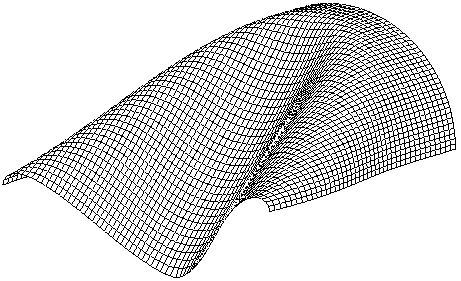
\includegraphics[width=\textwidth]{./Ressourcen/titleimage.pdf}
\end{figure}


\AddToShipoutPictureBG*{%
	\AtTextLowerLeft{\makebox[\textwidth][r]
		{%
			
\includegraphics[width=1.9cm]{./Ressourcen/Universitaet_Logo_RGB.pdf}
			\hspace{\fill}
			\includegraphics[width=2.37cm]{./Ressourcen/Statik.pdf}
		}
		}
		}

%\begin{textblock*}{\textwidth}[1,0](\textwidth-1mm, 2cm-\SeitenrandOben)%
%	\raisebox{-.5\height}{
\includegraphics[width=1.9cm]{./Ressourcen/Universitaet_Logo_RGB.pdf}}%
%	\hfill
%	\raisebox{-.5\height}{\includegraphics[width=2.37cm]{./Ressourcen/Statik.pdf}}%
%\end{textblock*}
%
%\includegraphics[width=4cm]{image1.eps}
%\hspace{\fill}
%\includegraphics[width=4cm]{image2.eps}

%\newpage

%\vspace*{-15.8mm}
%\fontsize{19pt}{21pt}\selectfont
%\ErklaerungUeberschrift
%
%\vspace{25.3mm}
%Erklärung
%
%\normalsize\selectfont
%\vspace{13.2mm}
%Ich versichere hiermit, dass ich die von mir eingereichte Abschlussarbeit selbstständig verfasst und keine anderen als die angegebenen Quellen und Hilfsmittel benutzt habe.
%
%\vspace{18.1mm}
%\rule[-3.7mm]{\linewidth}{0.5pt}
%\Ort{}, \Datum{}, Unterschrift

%\end{document}

\renewcommand{\SeitenrandOben}{25.8mm}
\renewcommand{\SeitenrandRechts}{21mm}
\renewcommand{\SeitenrandLinks}{40mm}
\renewcommand{\SeitenrandUnten}{24.8mm}

\restoregeometry
 % alternate title page


%%%%%%%%%%%%%%%%%%%%%%%%%%%%%%%%%%%%%%%%%%%%%%%%%%%%%%%%%%%%%%%%%%%%%%%%%%%%%%%%
% EINSTELLUNGEN
%%%%%%%%%%%%%%%%%%%%%%%%%%%%%%%%%%%%%%%%%%%%%%%%%%%%%%%%%%%%%%%%%%%%%%%%%%%%%%%%

% Seitenränder:
\renewcommand{\SeitenrandOben}{43.5mm}
\renewcommand{\SeitenrandRechts}{20mm}
\renewcommand{\SeitenrandLinks}{20mm}
\renewcommand{\SeitenrandUnten}{10mm}

\newcommand{\UniversitaetLogoBreite}{19mm}
\newcommand{\UniversitaetLogoHoehe}{1cm}

%\usepackage[a4paper,
%    top=\SeitenrandOben,
%    bottom=\SeitenrandUnten,
%    inner=\SeitenrandLinks,
%    outer=\SeitenrandRechts,
%    foot=0cm,
%    head=0cm
%]{geometry}

\newgeometry{
    top=\SeitenrandOben,
    bottom=\SeitenrandUnten,
    inner=\SeitenrandLinks,
    outer=\SeitenrandRechts,
    foot=0cm,
    head=0cm
}

\textblockorigin{\SeitenrandLinks}{\SeitenrandOben} % Ursprung für Positionierung

\setlength{\parindent}{0pt}
%\setlength{\baselineskip}{32pt}
\setlength{\parskip}{\baselineskip}
\TabPositions{4cm}
\pagestyle{empty}


%%%%%%%%%%%%%%%%%%%%%%%%%%%%%%%%%%%%%%%%%%%%%%%%%%%%%%%%%%%%%%%%%%%%%%%%%%%%%%%%
% DOKUMENT
%%%%%%%%%%%%%%%%%%%%%%%%%%%%%%%%%%%%%%%%%%%%%%%%%%%%%%%%%%%%%%%%%%%%%%%%%%%%%%%%

%\begin{document}


\begin{textblock*}{\UniversitaetLogoBreite}[1,0](\textwidth-1mm, 2cm-\SeitenrandOben)%
    \raggedleft
\includegraphics{./Ressourcen/Universitaet_Logo_RGB.pdf}%
\end{textblock*}


\begin{textblock*}{\textwidth}[0,0](0cm, 0cm)%
{\fontsize{24pt}{26pt}\selectfont\textbf{\Titel}}

\vspace*{14pt} %27
{\fontsize{18pt}{22pt}\selectfont\textbf{Formulation, Implementation, Validation \& Structural \\ Modelling}\par}
\end{textblock*}

\vspace*{92.2mm}

\ifx\lan\deutsch 

\fontsize{14.4pt}{17.5pt}\selectfont%
Wissenschaftliche Arbeit zur Erlangung des Grades\\
\Grad\\
an der \Fakultaet{} der Technischen Universität München.

\renewcommand{\baselinestretch}{1.47}
\normalsize\selectfont
\vspace*{17.1mm}
\textbf{Betreut von}\tab
\begin{minipage}[t]{\textwidth-\CurrentLineWidth}
	\BetreutVonPerson\\
	\BetreutVonLehrstuhl\strut
\end{minipage}

\vspace*{4.3mm}
\textbf{Eingereicht von}\tab
\begin{minipage}[t]{\textwidth-\CurrentLineWidth}
	\EingereichtVon
\end{minipage}

\vspace*{-1mm}
\textbf{Eingereicht am}\tab 
\begin{minipage}[t]{\textwidth-\CurrentLineWidth}
	München, den \Datum\strut
\end{minipage}

\else

\fontsize{14.4pt}{17.5pt}\selectfont%
Submitted to the \Fakultaet{}\\
in partial fulfillment of the requirements for the degree of\\
\Grad\\
at the Technical University of Munich.

\renewcommand{\baselinestretch}{1.47}
\normalsize\selectfont
\vspace*{17.1mm}
\textbf{Supervised by}\tab
%\begin{minipage}[t]{\textwidth-\CurrentLineWidth}
%	\BetreutVonPerson\\
%	\BetreutVonLehrstuhl\strut
%\end{minipage}
\begin{minipage}[t]{\textwidth-\CurrentLineWidth}
	Dipl.-Ing. (FH) Andreas Winterstein M.Sc. \\
	PD Dr.-Ing. habil. Roland W\"{u}chner \\
	Prof. Dr.-Ing. Kai-Uwe Bletzinger \\
	Chair of Structural Analysis
\end{minipage}

\vspace*{4.3mm}
\textbf{Submitted by}\tab
\begin{minipage}[t]{\textwidth-\CurrentLineWidth}
	\EingereichtVon
\end{minipage}

\vspace*{-1mm}
\textbf{Submitted on}\tab 
\begin{minipage}[t]{\textwidth-\CurrentLineWidth}
	Munich, \Datum\strut
\end{minipage}

\fi




\newpage

%\vspace*{-15.8mm}
%\fontsize{19pt}{21pt}\selectfont
%\ErklaerungUeberschrift
%
%\vspace{25.3mm}
%Erklärung
%
%\normalsize\selectfont
%\vspace{13.2mm}
%Ich versichere hiermit, dass ich die von mir eingereichte Abschlussarbeit selbstständig verfasst und keine anderen als die angegebenen Quellen und Hilfsmittel benutzt habe.
%
%\vspace{18.1mm}
%\rule[-3.7mm]{\linewidth}{0.5pt}
%\Ort{}, \Datum{}, Unterschrift

%\end{document}

\renewcommand{\SeitenrandOben}{25.8mm}
\renewcommand{\SeitenrandRechts}{21mm}
\renewcommand{\SeitenrandLinks}{40mm}
\renewcommand{\SeitenrandUnten}{24.8mm}

\restoregeometry
 % cover sheet
\pagenumbering{gobble}
%%%%%%%%%%%%%%%%%%%%%%%%%%%%%%%%%%%%%%%%%%%%%%%%%%%%%%%%
%%%%                                              %%%%%%
%%%%  Author: Name des Autors                     %%%%%%
%%%%                                              %%%%%%
%%%%  Beschreibung:                               %%%%%%
%%%%                                              %%%%%%
%%%%%%%%%%%%%%%%%%%%%%%%%%%%%%%%%%%%%%%%%%%%%%%%%%%%%%%%

\chapter*{Abstract}
\label{cha:abstract}
\lettrine[lines=2]{A}{s} the use of Finite Element Analysis (FEA) proliferates throughout both academia and industry so does the need to curb ill-conceived shell finite element analyses. Exacerbated by the prevalence of commercial "black box" codes, the ease with which ostensibly correct results can be obtained poses a unique risk compared to classical engineering methods. Advanced shell finite elements with enhancing element technologies, such as the linear triangle DSG and the linear quadrilateral ANDES-DKQ elements implemented and validated in this thesis, have proven themselves robust enough for general purpose analysis and no doubt aid in tempering the risk of incorrect analysis. However, simply employing advanced shell finite elements does not automatically inoculate against spurious analyses. Correct understanding of shell theories and the shell finite elements themselves gives rise to the correct structural modelling of shell finite elements, a detailed study of which is presented in this work. Consolidation of advanced shell finite elements and their proper structural modelling effectively mitigates this risk, resulting in confident and accurate analyses.

\vspace*{10mm}

%\section*{Keywords}
{\textcolor{gray75}{\Huge\bfseries{Keywords}}}

\vspace*{8mm}

\keywords
%{\textcolor{gray75}{\Huge\bfseries{Keywords}}}

\newpage
%\include{chapters/Acknowledgements}	%optional
\newpage
\pagenumbering{Roman}
\setcounter{tocdepth}{1}
\renewcommand{\cftchapafterpnum}{\vspace{\cftbeforechapskip}}
\tableofcontents
\mainmatter %turns on chapter numbering, resets page numbering
\pagenumbering{arabic}
\pagestyle{headings}

%TOEDIT create different files for your chapter an include them here in the main file

\setlength{\belowcaptionskip}{-17pt}

%%%%%%%%%%%%%%%%%%%%%%%%%%%%%%%%%%%%%%%%%%%%%%%%%%%%%%%%
%%%%                                              %%%%%%
%%%%  Author: Peter Wilson                        %%%%%%
%%%%                                              %%%%%%
%%%%  Introduction                                %%%%%%
%%%%                                              %%%%%%
%%%%%%%%%%%%%%%%%%%%%%%%%%%%%%%%%%%%%%%%%%%%%%%%%%%%%%%%


%fref generates automatically the respective abreviation/word in the text for the reference. You just have to define a label starting with the respective keyword.
%english: chap, sec, fig, eq, app
%deutsch: chap/kap, abs, abb, gl, anh
%see http://ctan.space-pro.be/tex-archive/macros/latex/contrib/fancyref/fancyref.pdf for more information

\chapter{Introduction}
\label{chap:chapter_1}

\renewcommand{\Thema}{Introduction}

\lettrine[lines=2]{T}{he} increasing use of the Finite Element Method (FEM) in both academia and the industry is driven by a myriad of competing external pressures such as greater strength vs. leaner designs and quicker analysis yielding increased accuracy. Many engineering scenarios previously analysed with classical hand calculations are now finalized or replaced with the use of Finite Element Analysis (FEA), or, indeed, the aforementioned pressures drive designs into new realms that fall outside the purview of hand calculations entirely. Detailed analysis of conventional structural steelwork and innovative design of unconventional lightweight shell structures are but two examples of the widespread embrace of FEA, both of which commonly employ shell finite elements to accurately resolve structural behaviour. Given the availability of "black box" commercial FEM codes and the ease with which ostensibly convincing shell models can be created, a general lack of shell theory knowledge manifests a void subsequently filled with questionable results. Conversely, shell theory knowledge allows one to appreciate both the critical behaviour of the structure and also realise the limitations of various shell finite elements, the reconciliation of these two items in conjunction with advanced robust shell finite elements culminates in confident and accurate analyses.

The objective of this work is two-fold:
\begin{enumerate}
	\item Implement two advanced shell finite elements in the multi-physics code Kratos with the following functionality:
	\begin{itemize}
		\item isotropic and orthotropic laminate linear elastic materials,
		\item geometrically linear and non-linear analysis,
		\item static and dynamic analysis, and,
		\item generous quantity recovery options.\\
	\end{itemize}

	\item Illuminate the structural modelling of advanced shell finite elements by examining the interaction between structural behaviour, base formulations, enhancing technologies and formulation-mesh-dependency.
\end{enumerate}


\newpage
This thesis can be divided into three parts:
\begin{itemize}
	\item \textbf{Part 1: Background theory}
	
	Chapters 2 - 4 cover the relevant theory pertinent not only to the implementation of the shells in Kratos, but also to the theoretical understanding necessary for an informed discussion of shell structural modelling.
	\begin{itemize}
		\item Chapter 2 provides an overview of common mathematical shell models and their associated assumptions and limitations. Artificial locking effects that arise from the translation of these mathematical models into low order finite elements are discussed, as well as various element technologies proposed as remedies. From this, the base formulations and enhancement technologies of the Kratos elements to be implemented are chosen.
		\item Chapter 3 establishes composite material basics and common composite nomenclature. The internal work of a 5-parameter orthotropic laminate shell is developed, leading to expressions for the integrated laminate constitutive matrix and integrated force resultants. Laminae stress and strain recovery are subsequently covered, followed by the Tsai-Wu failure criterion.
		\item Chapter 4 covers a general overview of non-linear analysis. Response diagrams and critical points are explored through the lens of stability analysis, while an outline of the co-rotational approach and the element independent co-rotational approach, used in Kratos, are subsequently offered.
	\end{itemize}


	\item \textbf{Part 2: Implementation of shells in Kratos}
	
	Chapters 5 - 8 primarily deal with the implementation of the advanced shell elements in Kratos and their validation.
	\begin{itemize}
		\item Chapter 5 walks through the DSG linear triangle shell element formulation and implementation in Kratos. The stiffness matrix formulation and implementation, lumped and consistent mass matrix details and stress and strain recovery are covered.
		\item Chapter 6 goes through the ANDES-DKQ linear quadrilateral shell element formulation and implementation in Kratos, surveying the same points as chapter 5.
		\item Chapter 7 extends both elements from isotropic materials to orthotropic composite laminates by covering the relevant constitutive matrices, stress and strain recovery and Tsai-Wu failure criterion details.
		\item Chapter 8 demonstrates the correct implementation and accuracy of the elements with validation tests spanning linear statics, non-linear statics, linear dynamics and non-linear dynamics across isotropic and orthotropic composite materials. Recovery of stresses, strains, integrated forces, Von Mises stresses and the composite Tsai-Wu reserve index are also validated.
	\end{itemize}
	\newpage
	\item \textbf{Part 3: Finite element structural modelling}
	
	Chapters 9 and 10 examine the structural modelling of finite shell elements, interrogating the interplay between structural behaviour, base formulations, enhancing technologies and formulation-mesh-dependency.
	\begin{itemize}
		\item Chapter 9 considers the detailed interrogation of two geometrically non-linear example problems: Euler beam buckling and the shear wrinkling of a flat plate. For each case the structural behaviour is compared across elements of different base formulations, with enhancing technologies switched on and off to further extricate the underlying phenomena either properly or improperly resolved by the various shell structural models.
		\item Chapter 10 looks at the extension of DSG linear triangle element technology into a formulation invariant of nodal numbering. A developmental proof of concept is considered, followed by a published DSG extension formulation whose behaviour does not depend on nodal ordering. Tying back to structural modelling, an appraisal of the DSG formulations is put forth with the aim of recommending the preferred DSG element for general analysis.
	\end{itemize}
\end{itemize}


The programming work associated with this thesis was completed in Kratos (links below), a multi-physics code with a plethora of individual applications including Structural Mechanics, Fluid Dynamics, Fluid Structure Interaction, Discrete Element Modelling and Shape Optimization, many of which can be combined seamlessly into multi-disciplinary analyses. Emerging from the International Center for Numerical Methods in Engineering (CIMNE) in Barcelona and co-developed by the Technical University of Munich (TUM), Kratos's applications are primarily written in C++ (the primary language of this work), while Python is also utilised for efficient communication between applications and with the user.

\vspace*{10mm}

\begin{figure}[H]
	\centering
	\def\svgwidth{\columnwidth}
	
\includegraphics[width=10cm]{images/kratoslogo.png}
	\label{kratoslogo}
\end{figure}

\begin{center}
CIMNE Kratos Multi-physics homepage: \\
\textit{http://www.cimne.com/kratos/}

Kratos Multi-physics Github: \\
\textit{https://github.com/KratosMultiphysics}

Kratos Multi-physics Github wiki, application cases: \\
 \textit{https://github.com/KratosMultiphysics/Kratos/wiki/Application-Cases}
\end{center} %intro
%%%%%%%%%%%%%%%%%%%%%%%%%%%%%%%%%%%%%%%%%%%%%%%%%%%%%%%%
%%%%                                              %%%%%%
%%%%  Author: Peter Wilson                        %%%%%%
%%%%                                              %%%%%%
%%%%  Background of shells                        %%%%%%
%%%%                                              %%%%%%
%%%%%%%%%%%%%%%%%%%%%%%%%%%%%%%%%%%%%%%%%%%%%%%%%%%%%%%%


%fref generates automatically the respective abreviation/word in the text for the reference. You just have to define a label starting with the respective keyword.
%english: chap, sec, fig, eq, app
%deutsch: chap/kap, abs, abb, gl, anh
%see http://ctan.space-pro.be/tex-archive/macros/latex/contrib/fancyref/fancyref.pdf for more \section

\renewcommand{\Thema}{Plates and shells}

\chapter{Plates and shells}
\label{chap:chapter_2}

\lettrine[lines=3]{T}{he} employment of shell structures is ubiquitous throughout both nature and the built environment. Eggs, nuts, blood vessels and cell walls are examples of shell designs being the result of structural optimisation via natural evolution over millennia. It is no doubt that man drew inspiration from the optimal natural shell design and quickly realised the efficacy of the shell structure, perhaps the pre-eminent example of early shell structures is the Roman Pantheon (126).  Throughout time, as the understanding of the structures increased, so did their prevalence, leading to notable structures such as the Hagia Sophia (537), Notre Dame (1345) and St. Peter's Basilica (1626). Indeed, the efficiency of shell structures lies in their high in-plane (membrane) load carrying capacity in slender low-weight constructions. The membrane action serves to stress all fibres approximately equally in the cross section, realising the full mechanical performance of the structure. Contrasting this, shells are incredibly sensitive to a variety of effects such as imperfections, bending, transverse normal forces and support conditions, leading to significant compromise of the membrane structural performance, possibly manifesting in catastrophic failure. Bending actions result in a non-uniform stressing of material fibres over the cross section, with the outer fibres stressed significantly more than those closer to the neutral axis. Consequently, the limit of the structure in bending is realised when only the outer-most fibre fails instead of the entire cross section of fibres failing under membrane action. This basic example offers a snapshot of the stellar performance of shells juxtaposed against their sensitivity to a multitude of conditions, earning them the title of the \textit{Prima Donna of structures} \cite{Ram16}.

\section{Structural modelling with shells}
Although shells present the opportunity of an optimally loaded structure, their delicate position in a sharply varying landscape of performance demands consideration of phenomena critical to the analysis undertaken. Contrasting this to the engineering design ethos of \textit{everything should be made as simple as possible, but no simpler}, the arising tension is immediately recognized, one that can only be curtailed by an in depth knowledge of the working problem and shells themselves. Within the engineering design context of a particular scenario, there exists as many opportunities to reduce complexity as there are to incorrectly exclude critical phenomena. Typical structural modelling decisions such as: inclusion or exclusion of inertial and damping effects, non-linear or linear material models, large or small deformation assumptions and dimensional reduction are examples of large brush strokes limiting the canvas of possibilities resolved. Focussing on the rendering of shells, the structural models assumed determine the behaviour they can exhibit. \\

Inherent in the use of shells in structural models is the concept of dimensional reduction from 3 dimensions to 2 dimensions, relying on the assumption that one dimension (thickness) is significantly smaller than the other two (length and width). 

\begin{figure}[H]
	\centering
	\def\svgwidth{\columnwidth}
	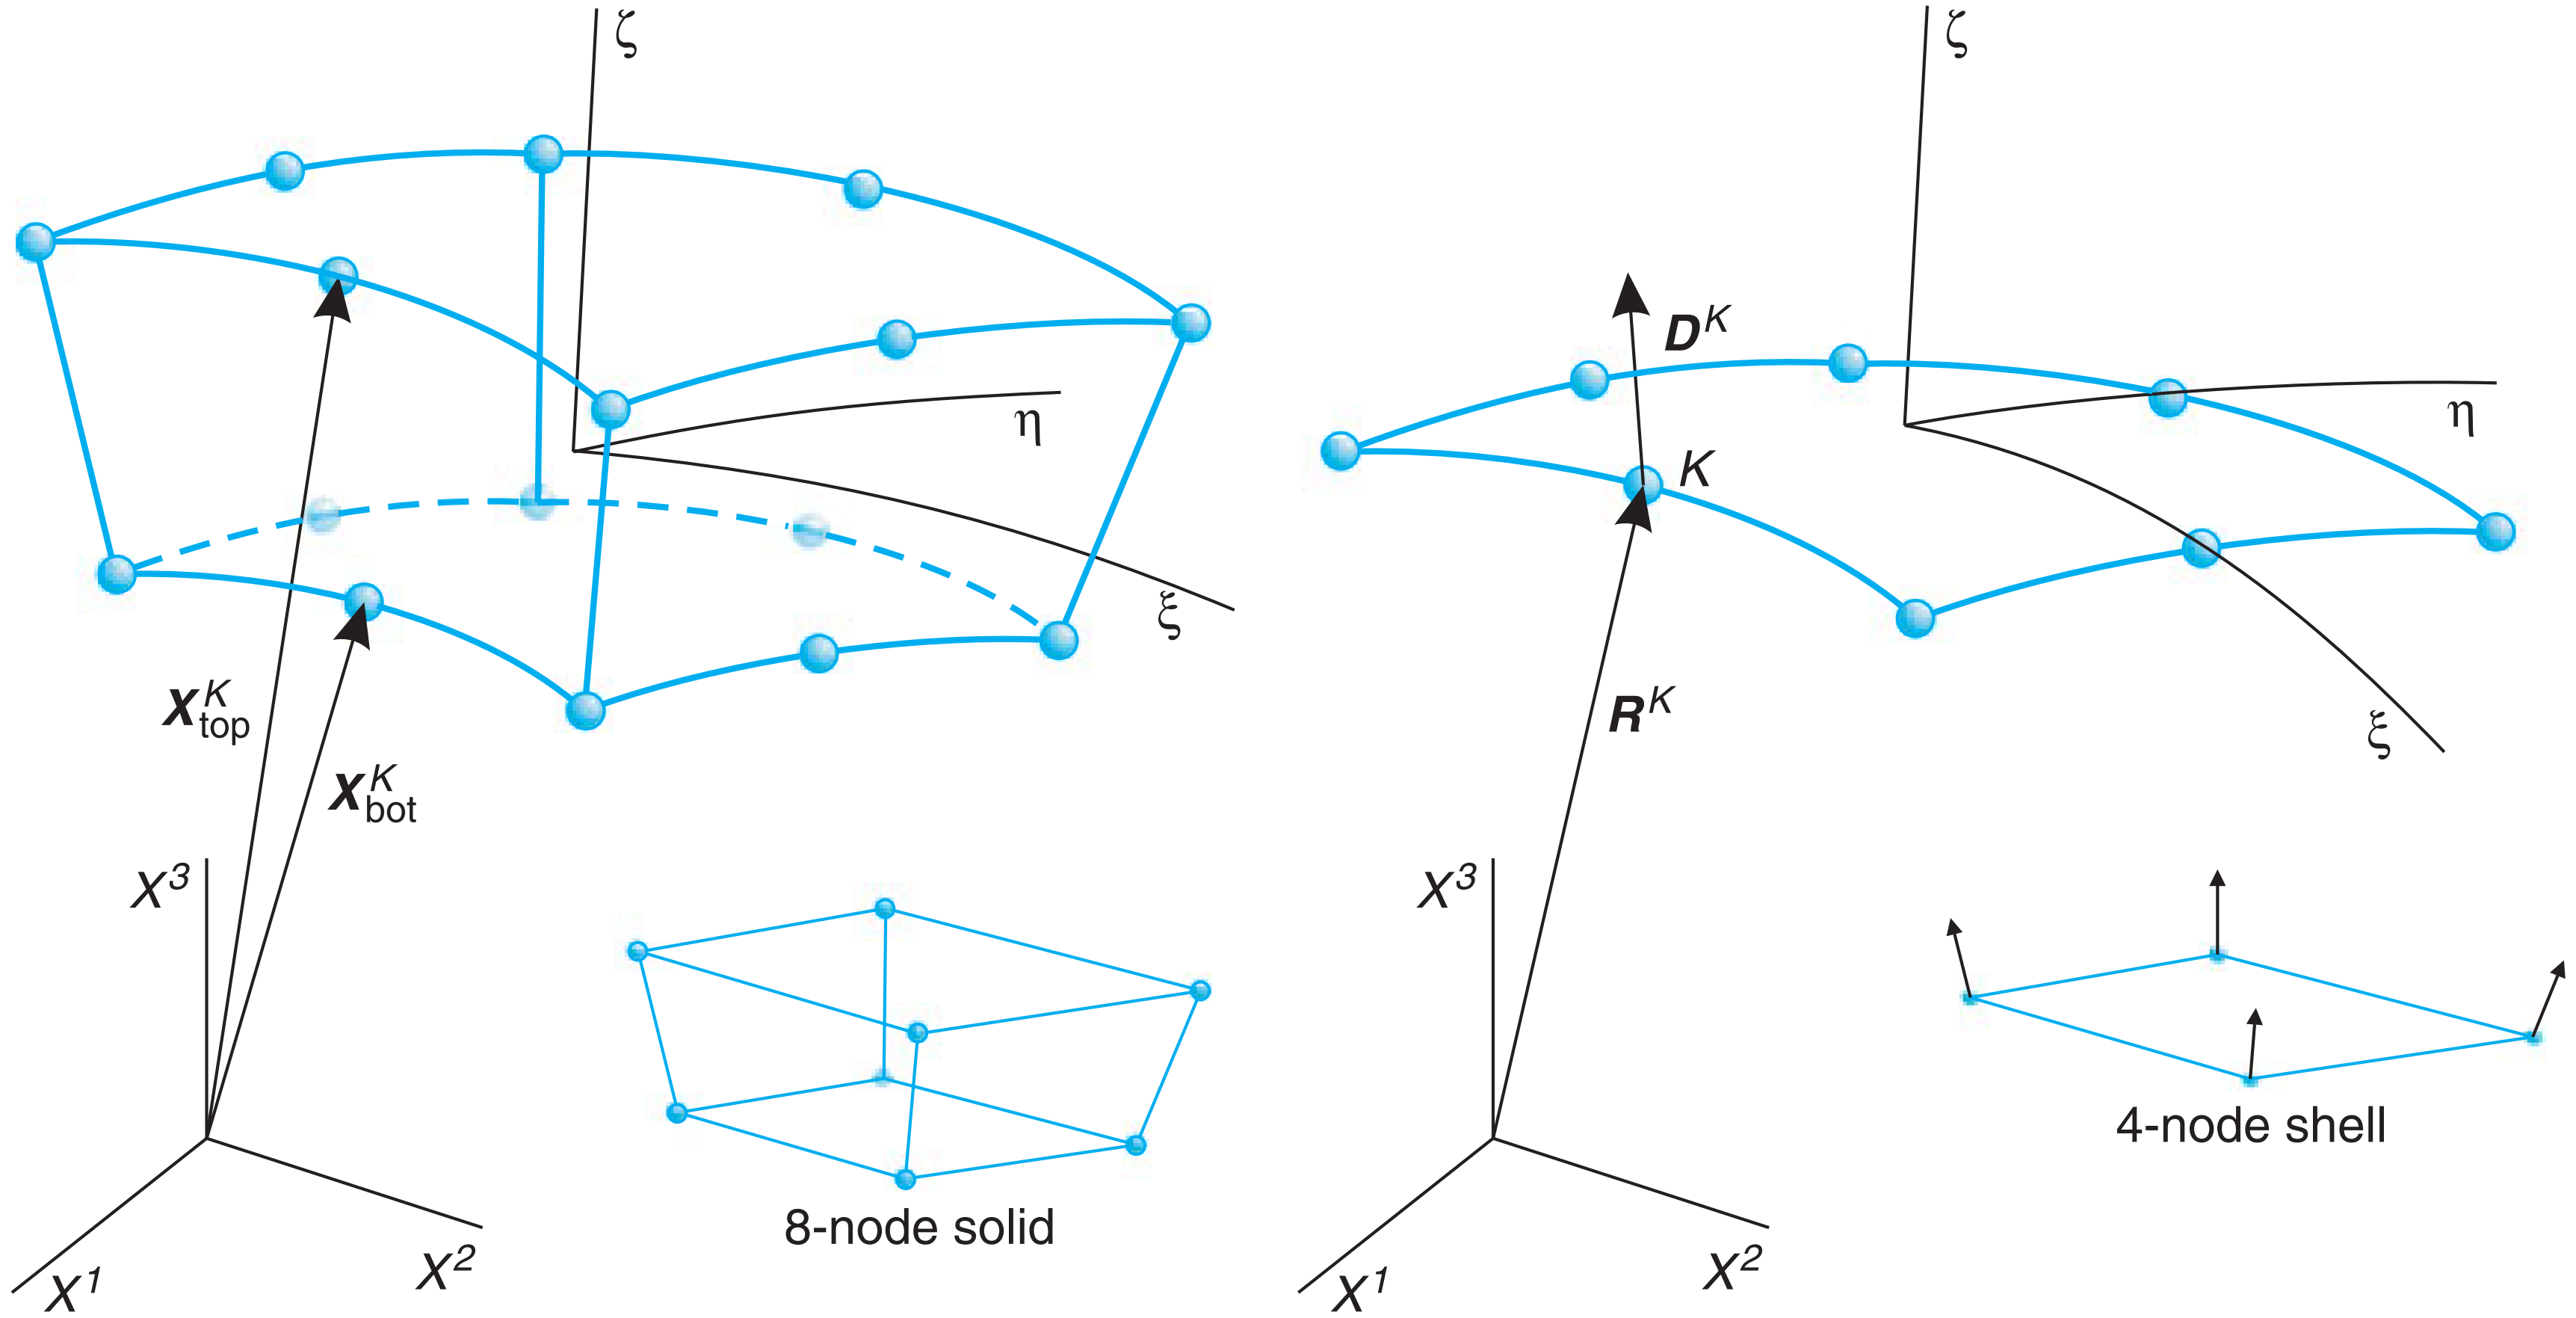
\includegraphics[width=12cm]{images/degenerateshell.png}
	\caption{Dimensional reduction of a solid to a shell \cite{BischLitBook04}}
	\label{shellModels}
\end{figure}

Already, it is apparent that the through-thickness response of the shell now must be modelled instead of resolved, with the results now a function of the approximation employed. This apparent simplification promptly begs a key question: what shall the model consider such that it is simple as possible, but not simpler? Can the thickness vary under deformation? Is the shell one uniform material or multi-layered? Is shear deformation of the thickness negligible or not? One may also impose far stricter modelling assumptions by only considering the bending or membrane behaviour of the shell. These common structural modelling decisions, amongst others, have yielded typical shell models.

\section{Shell models}

Commencing in the Renaissance and continuing into the present day, the mathematical development of shell models has facilitated the construction of increasingly elaborate shell structures. The main mathematically-based shell models considered in this work are illustrated below.

\begin{figure}[H]
	\centering
	\def\svgwidth{\columnwidth}
	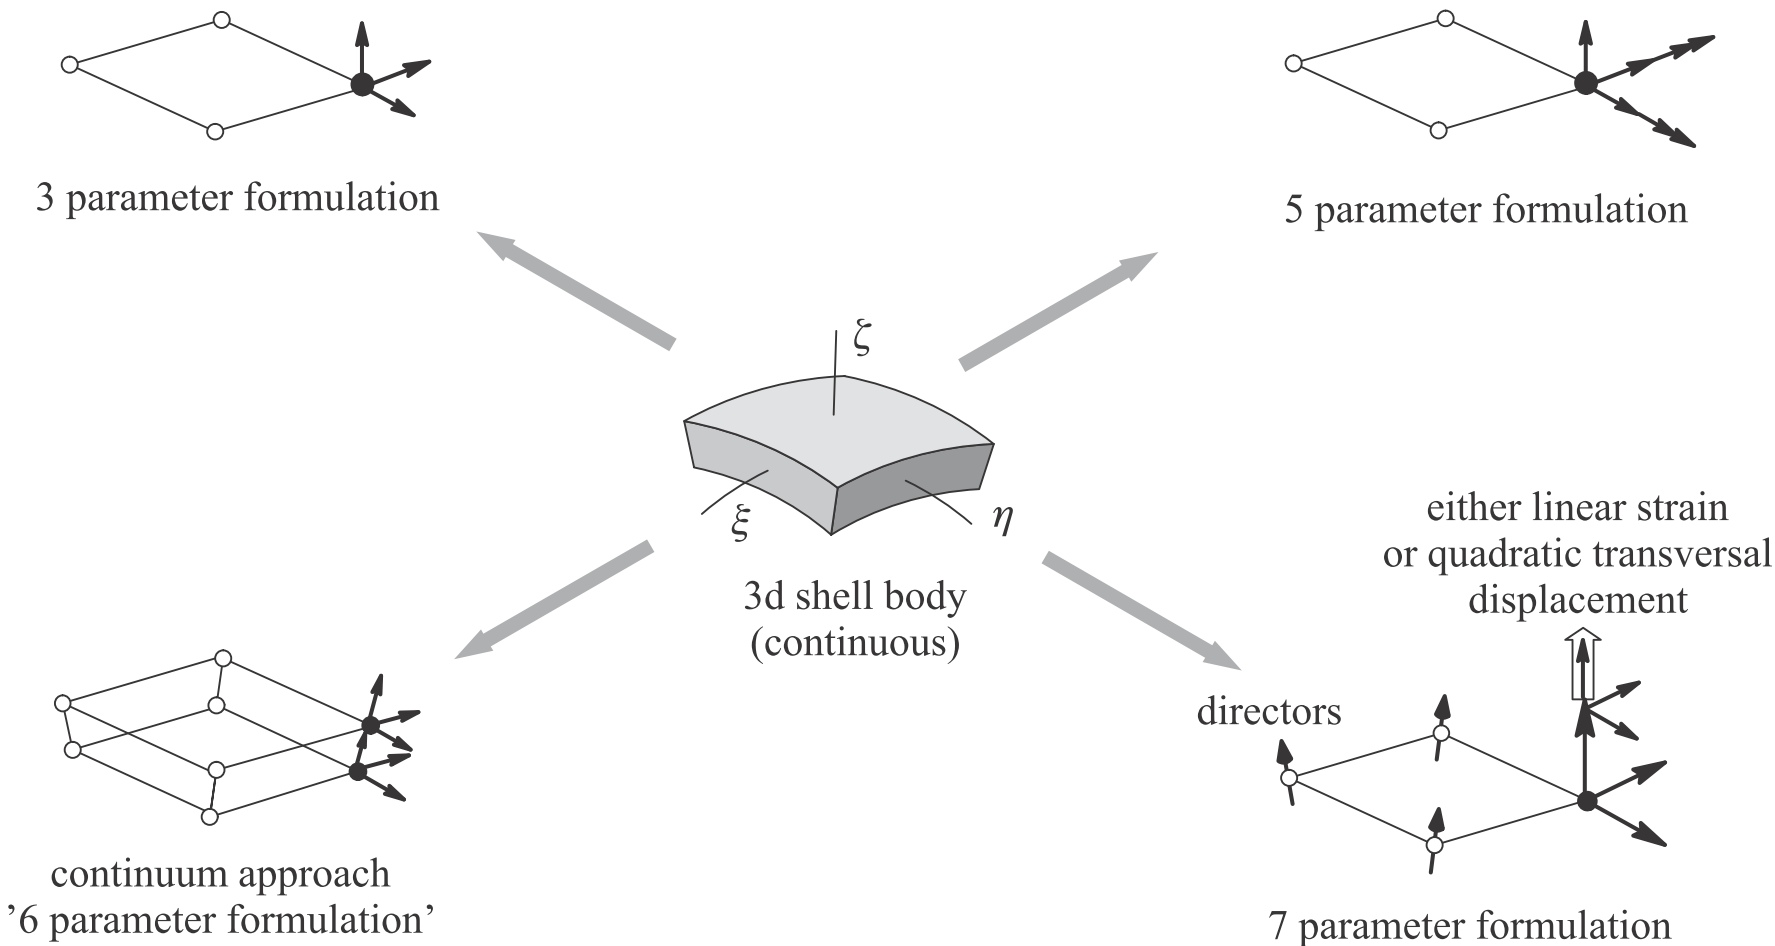
\includegraphics[width=12cm]{images/shellModels.png}
	\caption{Various shell models \cite{Wall2000}}
	\label{shellModels}
\end{figure}

Each of the shell models above are based on different assumptions and physics, which essentially act as a filter of what phenomena the structural model can resolve. These models, as well as the basic membrane model, will be briefly discussed in the following section (further details can be found in References \cite{BischLitBook04} \cite{RammLitBook04} ans \cite{Echter13}). To gain further insight, high level formulations of the models are presented with a focus of the mathematical representation of the key assumptions.  The follow figure illustrates the configurations and notation of the formulations. 

\begin{figure}[H]
	\centering
	\def\svgwidth{\columnwidth}
	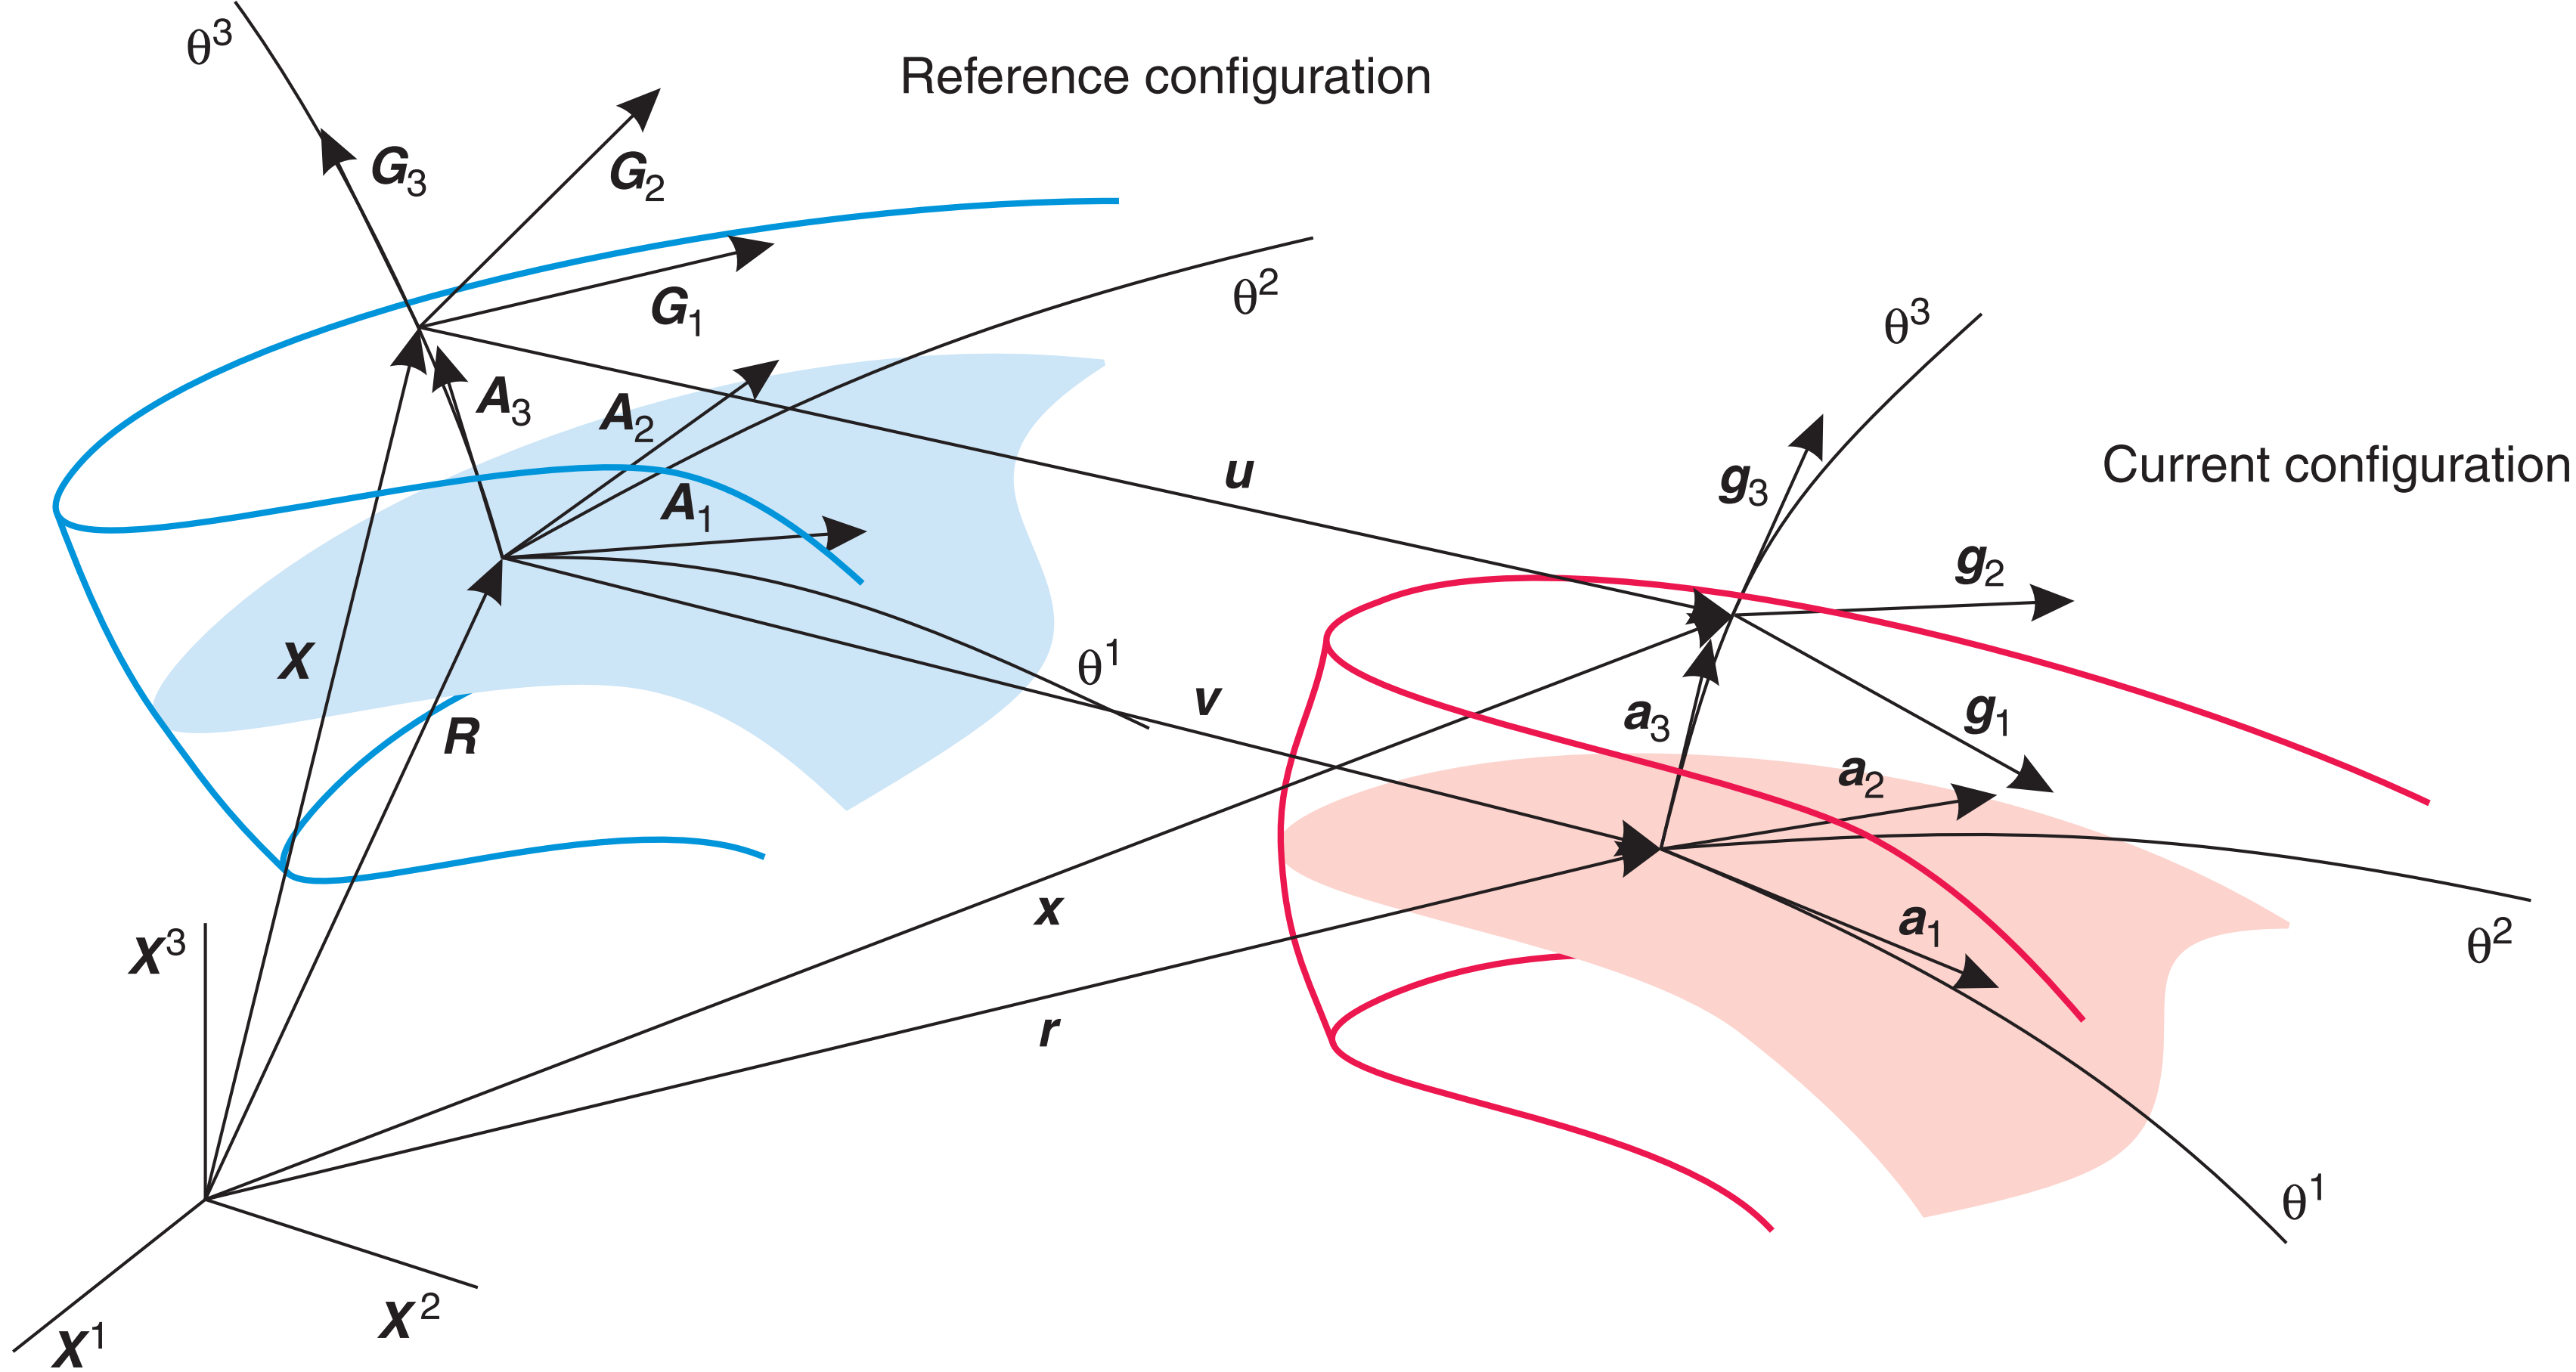
\includegraphics[width=12cm]{images/shellsconfig.png}
	\caption{Deformation, reference and current configuration \cite{BischLitBook04}}
	\label{shellsconfig}
\end{figure}

Quantities in the reference configuration are expressed in upper case while quantities in lower case are in the deformed configuration. The reference shell mid-plane $\theta^3 = 0$ position vector of a point is denoted $\mathbf{R}$, while an arbitrary point is denoted $\mathbf{X}$. Correspondingly, base vectors on the mid-plane are denoted $\mathbf{A}_i$ and $\mathbf{a}_i$ while $\mathbf{G}_i$ and $\mathbf{g}_i$ denote arbitrary base vectors. It is noted that Einstein notation is employed here, with Latin characters corresponding to summation over three dimensions while Greek characters sum over two dimensions. Lastly, $\mathbf{v}$ and $\mathbf{u}$ indicate displacements on the mid-plane and arbitrary location respectively.


\subsection{Membrane model}

Despite not truly being a shell model, the membrane model is the simplest model available due to the complete ignorance of bending behaviour. Thus, the structural behaviour of the whole element is described by in plane components. Typically it is assumed that all stress and strain components are constant over the thickness. A key model choice is the specification of either plane stress or plane strain behaviour which is implemented in material matrix. \\

Commencing a high level formulation of the membrane model, the assumption of constant strain and stress components over the thickness allows collapsing the body into an infinitely thin shell. Thus thickness can be ignored in the position vectors.

\begin{equation} 
\mathbf{X} = \mathbf{R}\ ,
\hspace{10mm}
\mathbf{x} = \mathbf{r}\ ,
\hspace{10mm}
\mathbf{r} = \mathbf{R} + \mathbf{v}
\label{eqsmem1a}
\end{equation}

Using the notation of $(\ )_{,\alpha} = \frac{\partial(\ )}{\partial	\alpha}$ and explicitly writing the base vectors of the coordinate system yields:

\begin{equation} 
\mathbf{A}_\alpha  = \mathbf{R}_{,\alpha} =  \mathbf{X}_{,\alpha}
\ ,
\hspace{10mm}
\mathbf{a}_\alpha  = \mathbf{r}_{,\alpha} = \mathbf{A}_\alpha + \mathbf{v}_{,\alpha}
\label{eqsmem1b}
\end{equation}

Considering the metrics of the reference and deformed configuration, the in-plane Green-Lagrange strain components read:

\begin{equation} 
\epsilon_{\alpha\beta} = \frac{1}{2}
(a_{\alpha\beta} - A_{\alpha\beta})
\hspace{10mm}
with
\hspace{10mm}
a_{\alpha\beta} = \mathbf{a}_\alpha \cdot \mathbf{a}_\beta
\hspace{10mm}
A_{\alpha\beta} = \mathbf{A}_\alpha \cdot \mathbf{A}_\beta
\label{eqsmem2}
\end{equation}

Corresponding to the membrane assumptions, all out of plane strain components are 0.

\begin{equation} 
\epsilon_{3i} = 0
\label{eqsmem3}
\end{equation}

At this point, one notices that all strain terms are completely contained within the two in-plane mid-surface displacements $\mathbf{v}_\alpha$. \\

By introducing the elasticity tensor $\mathbf{C}_0$ (typically plane stress) the stress components can be recovered from the strains.

\begin{equation} 
\sigma^{\alpha\beta} = C_0^{\alpha\beta\gamma\delta} \epsilon_{\gamma\delta}
\label{eqsmem4}
\end{equation}

With stresses and strains determined, the internal and a generalised external virtual (where $\mathbf{f}$ is a generalised traction vector and $\delta \mathbf{v}$ are virtual displacements) can be expressed:

\begin{equation} 
-\delta\Pi_{int} = 
\int_\Omega
\boldsymbol{\epsilon}
:
\mathbf{C}_{mem}
:
\delta \boldsymbol{\epsilon}\ 
d \Omega\ ,
\hspace{10mm}
\delta\Pi_{ext} = \int_\Omega
\mathbf{f}^T
\delta  \mathbf{v}\ 
d \Omega
\label{eqsmem5}
\end{equation}

%Condensing to vector notation the above yields:
%
%\begin{equation} 
% \boldsymbol{\epsilon} =  \begin{pmatrix}
%  \epsilon_{xx} \\
%  \epsilon_{yy} \\
%  2\epsilon_{xy} \\
% \end{pmatrix} 
% \hspace{10mm}
% \mathbf{C}_0 = \frac{E}{1-\nu^2} \bar{\mathbf{C}} = \frac{E}{1-\nu^2}
% \begin{pmatrix}
%  1 & 0 & 0 \\
%   0 & 1 & 0 \\
%    0 & 0 & \frac{1-\nu}{2}
% \end{pmatrix} 
%\label{eqsmem7}
%\end{equation}

%\begin{equation} 
%\delta\Pi_{ext} = \int_\Omega
% \mathbf{f}^T
%\delta  \mathbf{v}\ 
%d \Omega
%\label{eqsmem7}
%\end{equation}

It's apparent that the internal work is composed solely of in-plane action, corresponding to the general descriptive assumptions of the membrane model above. By extension, it can be understood that the membrane model provides no resistance to out of plane action. Thus, unless the membrane-modelled structure is pre-stressed, the system will be rendered singular under out of plane loads. This lack of out of plane stiffness can also lead to buckling under compressive stresses. Considering the reduced phenomena that the membrane model can resolve, it is crucial to understand the critical physics of the system before employing it.

\subsection{3 parameter model: Kirchhoff-Love shell}

The first actual shell model considered is the 3 parameter model, often referred to as the Kirchhoff-Love (KL) shell. This model includes all membrane considerations, but also describes bending behaviour too. The bending behaviour is constrained to a description similar to the Bernoulli beam: shell directors across the thickness are always straight and normal to the mid-surface. Graphically, this is represented in the following figure:

\begin{figure}[H]
	\centering
	\def\svgwidth{\columnwidth}
	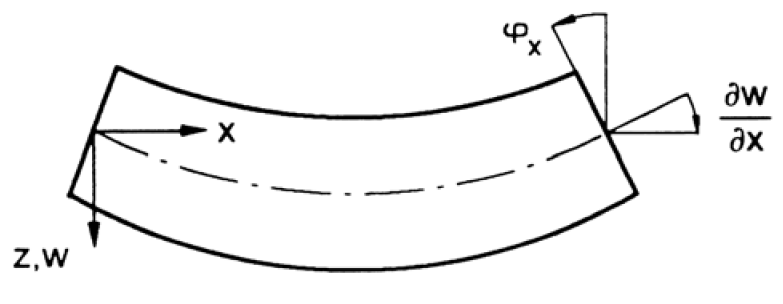
\includegraphics[width=8cm]{images/bernoullie.png}
	\caption{Kirchhoff-Love shell kinematics \cite{Bletz16}}
	\label{thinshellkine1}
\end{figure}

A consequence of the above kinematics is that this model ignores transverse shear strains. Thus, the applicability of the 3 parameter model is clearly limited to thin plates in the range of $\frac{1}{5} < \frac{l}{t} < \frac{1}{50}$ where transverse deformations are negligible. Similar to the membrane model, thickness deformation is ignored. \\

Establishing the geometry of the KL shell requires incorporation of the shell director along $\theta^3$ in the reference $\mathbf{D}$ and deformed configuration $\mathbf{d}$.

\begin{equation} 
\mathbf{X} = \mathbf{R} + \theta^3 \mathbf{D}\ ,
\hspace{10mm}
\mathbf{x} = \mathbf{r} + \theta^3 \mathbf{d}\ ,
\hspace{10mm}
\mathbf{r} = \mathbf{R} + \mathbf{v}\ ,
\hspace{10mm}
\mathbf{d} = \boldsymbol{\Lambda}  \mathbf{D}
\label{eqskt1}
\end{equation}

The above equation enforces the KL condition of a straight director with the linear description of $\theta^3 \mathbf{d}$. $\boldsymbol{\Lambda}$ is a rotation tensor composed of two independent rotation parameters $\beta^\alpha$ relating the reference and deformed directors to each other. In a Cartesian frame the linearised rotation components are: $\beta^1 = \mathbf{v}_{3,2}$ and $\beta^2 = -\mathbf{v}_{3,1}$ \cite{BischLitBook04}.  \\

The displacement is thus expressed:

\begin{equation} 
\mathbf{u} = \mathbf{x} - \mathbf{X}
=
\mathbf{v} + \theta^3 (\boldsymbol{\Lambda} - \mathbf{G}) \mathbf{D}
=
\mathbf{v} + \theta^3 \mathbf{d}
\label{eqskt2}
\end{equation}

!!!!!!!!!!!!!!!!!!!!!!!!!!!!!
Gotta figure out lamda - G = lamda
!!!!!!!!!!!!!!!!!!!!!!!!!!!!! \\

The KT requirement of the director being normal to the mid surface is expressed via the following dot product:

\begin{equation} 
\mathbf{d} \cdot \mathbf{r}_{,\alpha}
=
(\boldsymbol{\Lambda} \mathbf{D}) \cdot (\mathbf{A}_\alpha + \mathbf{v}_{,\alpha})
=
0
\label{eqskt3}
\end{equation}

Explicitly writing the base vectors of the coordinate system:

\begin{equation} 
\mathbf{A}_\alpha  = \mathbf{R}_{,\alpha}
\hspace{10mm}
\mathbf{a}_\alpha  = \mathbf{r}_{,\alpha} = \mathbf{A}_\alpha + \mathbf{v}_{,\alpha}
\label{eqskt4}
\end{equation}

Eqn \eqref{eqskt3}, requiring the director to be normal to the mid-surface, is guaranteed by employing cross products of the base vectors to construct the directors:

\begin{equation} 
\mathbf{D} = \frac{\mathbf{A}_1 \times \mathbf{A}_2}
{\lvert \lvert \mathbf{A}_1 \times \mathbf{A}_2 \rvert \rvert}
= \mathbf{A}_3\ ,
\hspace{10mm}
\mathbf{d} = \frac{\mathbf{a}_1 \times \mathbf{a}_2}
{\lvert \lvert \mathbf{a}_1 \times \mathbf{a}_2 \rvert \rvert}
= \mathbf{a}_3\ ,
\label{eqskt5}
\end{equation}

As the KT model considers bending, which is related to curvature, the second fundamental form of the system is defined in the reference and deformed configuration:

\begin{equation} 
B_{\alpha \beta} = \frac{1}{2} 
( 
\mathbf{A}_\alpha \cdot \mathbf{A}_{3,\beta} 
+
\mathbf{A}_\beta \cdot \mathbf{A}_{3,\alpha}
)
=
\mathbf{A}_\alpha \cdot \mathbf{A}_{3,\beta}
=
\mathbf{A}_\alpha \cdot \mathbf{D}_{,\beta}
\label{eqskt6}
\end{equation}

\begin{equation} 
b_{\alpha \beta} = \frac{1}{2} 
( 
\mathbf{a}_\alpha \cdot \mathbf{a}_{3,\beta} 
+
\mathbf{a}_\beta \cdot \mathbf{a}_{3,\alpha}
)
=
\mathbf{a}_\alpha \cdot \mathbf{a}_{3,\beta}
=
(\mathbf{A}_\alpha + \mathbf{v}_{,\alpha}) 
\cdot 
\Bigg({
	\frac{    (\mathbf{A}_1 + \mathbf{v}_{,1})  \times (\mathbf{A}_2 + \mathbf{v}_{,2})    }
	{\lvert \lvert  (\mathbf{A}_1 + \mathbf{v}_{,1})  \times (\mathbf{A}_2 + \mathbf{v}_{,2})   \rvert \rvert}
}\Bigg)_{,\beta}
\label{eqskt7}
\end{equation}

Contrasting to the membrane model, the KT strain tensor components now include linearly varying terms corresponding to bending phenomena:

\begin{equation} 
E_{\alpha \beta}
= \frac{1}{2}
(a_{\alpha\beta} - A_{\alpha\beta})
+
\theta^3 (b_{\alpha\beta} - B_{\alpha\beta})
=
\epsilon_{\alpha \beta} + \theta^3 \kappa_{\alpha \beta}
\label{eqskt8}
\end{equation}

According to the KT assumptions all out of plane strains are zero.

\begin{equation} 
E_{3i} = \epsilon_{3i} = \kappa_{3i} = 0
\label{eqskt81}
\end{equation}

Studying the strain components, especially the deformed second fundamental form, reveals that there are now 3 midplane displacements $\mathbf{v}_i$ involved in the description of the KT shell model, hence the name 3 parameter model. \\

Combining the above developments, and assuming the same general external work as equation \eqref{eqsmem5}, the internal virtual work can be presented:

\begin{equation} 
-\delta\Pi_{int} = 
\int_\Omega
\boldsymbol{\epsilon}
:
\mathbf{C}_{mem}
:
\delta \boldsymbol{\epsilon}\ d \Omega\ 
+
\int_\Omega
\boldsymbol{\kappa}
:
\mathbf{C}_{bend}
:
\delta \boldsymbol{\kappa}\ 
d \Omega
\label{eqskt9}
\end{equation}

The internal work equation illustrates the 3 parameter model considers in-plane membrane behaviour as well as the additional bending behaviour related to the second integral. Furthermore, under the condition of homogeneous linear material models the membrane and bending behaviour of the model are uncoupled. Due to the kinematics of the 3 parameter model (director remains straight and normal, no transverse shear strains), it can correctly resolve analyses as the thickness tends towards zero. This is in contrast the to 5 parameter model, which exhibits significant shear locking. Despite this, a pure rendition of the 3 parameter model is not commonly seen in practical FEM due to the required $C_1$ continuity at element boundaries (arising from rotations expressed as derivatives of transverse displacement) and the additional complication of effective shear forces on boundaries \cite{BischLitBook04}.


\subsection{5 parameter model: Reissner-Mindlin shell}

By relaxing the assumptions made in the 3 parameter shell model, the Reissner-Mindlin (RM) 5 parameter shell model can be derived. This model includes both membrane and bending action. While the KL model required that the shell directors remain normal to the mid-surface, the RM model relaxes this, analogous to the relationship between Bernoulli and Timoshenko beam models. Graphically, this is represented in the following figure:

\begin{figure}[H]
	\centering
	\def\svgwidth{\columnwidth}
	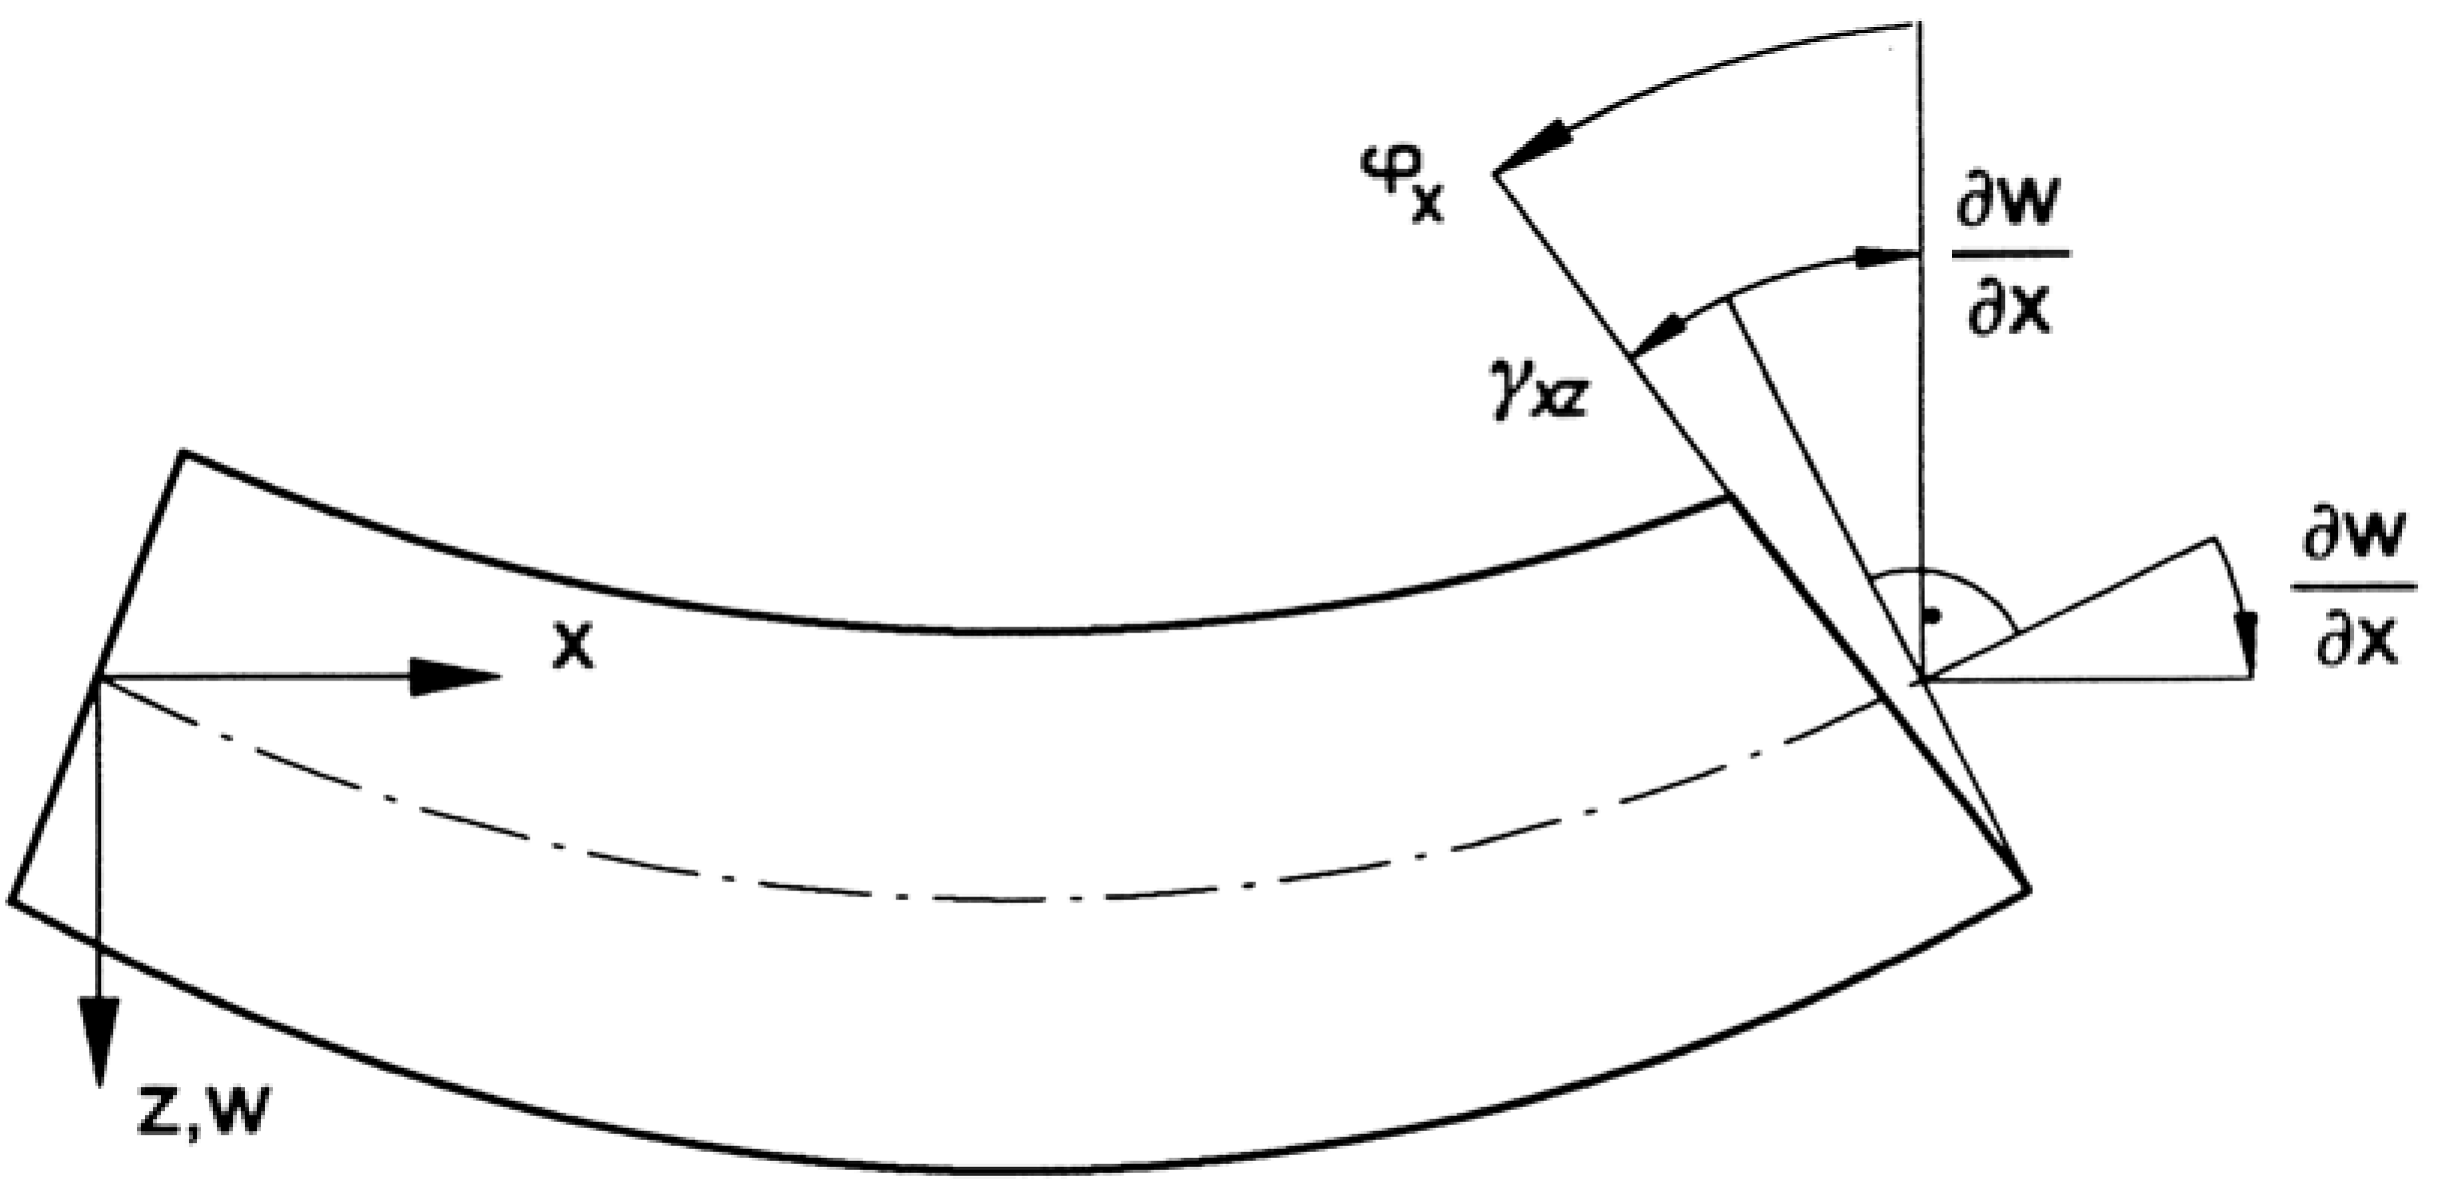
\includegraphics[width=8cm]{images/timoshenkobeam.png}
	\caption{Reissner-Mindlin shell kinematics \cite{Bletz16}}
	\label{thickshellkine1}
\end{figure}

Studying the above kinematics confirms this model now considers transverse shear strains, limiting the range of validity of this model to thick plates $\frac{1}{5} < \frac{l}{t} < \frac{1}{10}$ where transverse deformations are a key component of structural behaviour. Similar to the membrane and KL model, thickness deformation is ignored. \\

The geometry of the RM model is established similar to the KL model:

\begin{equation} 
\mathbf{u} = \mathbf{x} - \mathbf{X}
=
\mathbf{v} + \theta^3 (\boldsymbol{\Lambda} - \mathbf{G}) \mathbf{D}
=
\mathbf{v} + \theta^3 \mathbf{d}
\label{eqsrm1}
\end{equation}

However, the strict requirement of maintaining the director remain normal to the mid-surface, as expressed in the KL theory equation \eqref{eqskt3}, are no longer enforced. Correspondingly, the rotation tensor $\boldsymbol{\Lambda}$ must now include 2 additional parameters related to these 2 introduced degrees of freedom. \\

The general strain components are expressed as:

\begin{equation} 
E_{\alpha \beta}
= \frac{1}{2}
(a_{\alpha\beta} - A_{\alpha\beta})
+
\theta^3 (b_{\alpha\beta} - B_{\alpha\beta})
=
\epsilon_{\alpha \beta} + \theta^3 \kappa_{\alpha \beta}
\label{eqsrm2}
\end{equation}

Once again it is noted the assumption of straight directors is enforced by the linear coupling of $\theta^3 \kappa_{\alpha \beta}$. Following the assumption of no thickness strain, it is seen:

\begin{equation} 
E_{33} = \epsilon_{33} = \kappa_{33} = 0
\label{eqsrm21}
\end{equation}

By relaxing the director normality requirements, additional transverse shear strains must be accounted for:

\begin{equation} 
E_{\alpha 3} = E_{3 \alpha}
= \frac{1}{2}
(a_{\alpha 3} - A_{\alpha 3})
=
\frac{1}{2} \gamma_{3\alpha}
\label{eqsrm3}
\end{equation}

The internal virtual work is therefore expressed as:

\begin{equation} 
-\delta\Pi_{int} =
\int_\Omega
\boldsymbol{\epsilon}
:
\mathbf{C}_{mem}
:
\delta \boldsymbol{\epsilon}\ d \Omega\ 
+
\int_\Omega
\boldsymbol{\kappa}
:
\mathbf{C}_{bend}
:
\delta \boldsymbol{\kappa}\ 
d \Omega\ 
+
\int_\Omega
\boldsymbol{\gamma}
:
\mathbf{C}_{shear}
:
\delta \boldsymbol{\gamma}\ 
d \Omega
\label{eqsrm4}
\end{equation}

%\begin{equation} 
% \boldsymbol{\epsilon} =  \begin{pmatrix}
%  \epsilon_{xx} \\
%  \epsilon_{yy} \\
%  \epsilon_{xy} \\
% \end{pmatrix} 
% \hspace{10mm}
% \boldsymbol{\kappa} =  \begin{pmatrix}
%  \kappa_{xx} \\
%  \kappa_{yy} \\
%  2\kappa_{xy} \\
% \end{pmatrix} 
%  \hspace{10mm}
%  \boldsymbol{\gamma} =  \begin{pmatrix}
%  \gamma_{xz} \\
%  \gamma_{yz} \\
% \end{pmatrix} 
%\label{eqsrm6}
%\end{equation}

The 3 integrals of the virtual work equation represent the membrane, bending and shear work components, corresponding to the phenomena this model resolves. Furthermore, all these components are decoupled from each other in flat shells with homogeneous linear material models. The consideration of transverse shear deformations in the kinematics render the model applicable to thick shells where these strains are not insignificant. Incorrectly applying this model to thin shells in FEM yields spurious results due to a phenomena called shear locking (discussed in section \ref{transverse_shear_locking}). Despite this disadvantage, the 5 parameter forms the basis of many shell elements often used in FEM thanks to the lower $C_0$ continuity required at element boundaries.

\subsection{7 parameter model}

The previously discussed models all operate under the assumption that the transverse normal strains are zero. The 7 parameter model considers thickness deformation by introducing additional free parameters. Only a brief overview of the 7 parameter model is offered here as shell elements in FEM, the focus of this work, are predominately based off 3 and 5 parameter based formulations. For further details refer Bischoff et al. \cite{BischLitBook04} and Ramm and Wall \cite{RammLitBook04}. \\

Intuitively, one may realise that shell behaviour including thickness change may be described by 6 parameters:  3 mid-surface displacements, 1 thickness change and 2 rotations.  However, thickness locking occurs under this regime due to a mismatch of a linearly varying normal thickness stress $\theta^{33}$ conjugated with a constant thickness strain $\epsilon_{33}$. Thus the 7th parameter is the enhancement of the through thickness strain $\epsilon_{33}$ to a linear field. \\

It's clear that the additional modelling power of the 7 parameter shell can resolve physics that lower parameter models can't. A prime example of this is the Eigenvalue spectra presented below:

\begin{figure}[H]
	\centering
	\def\svgwidth{\columnwidth}
	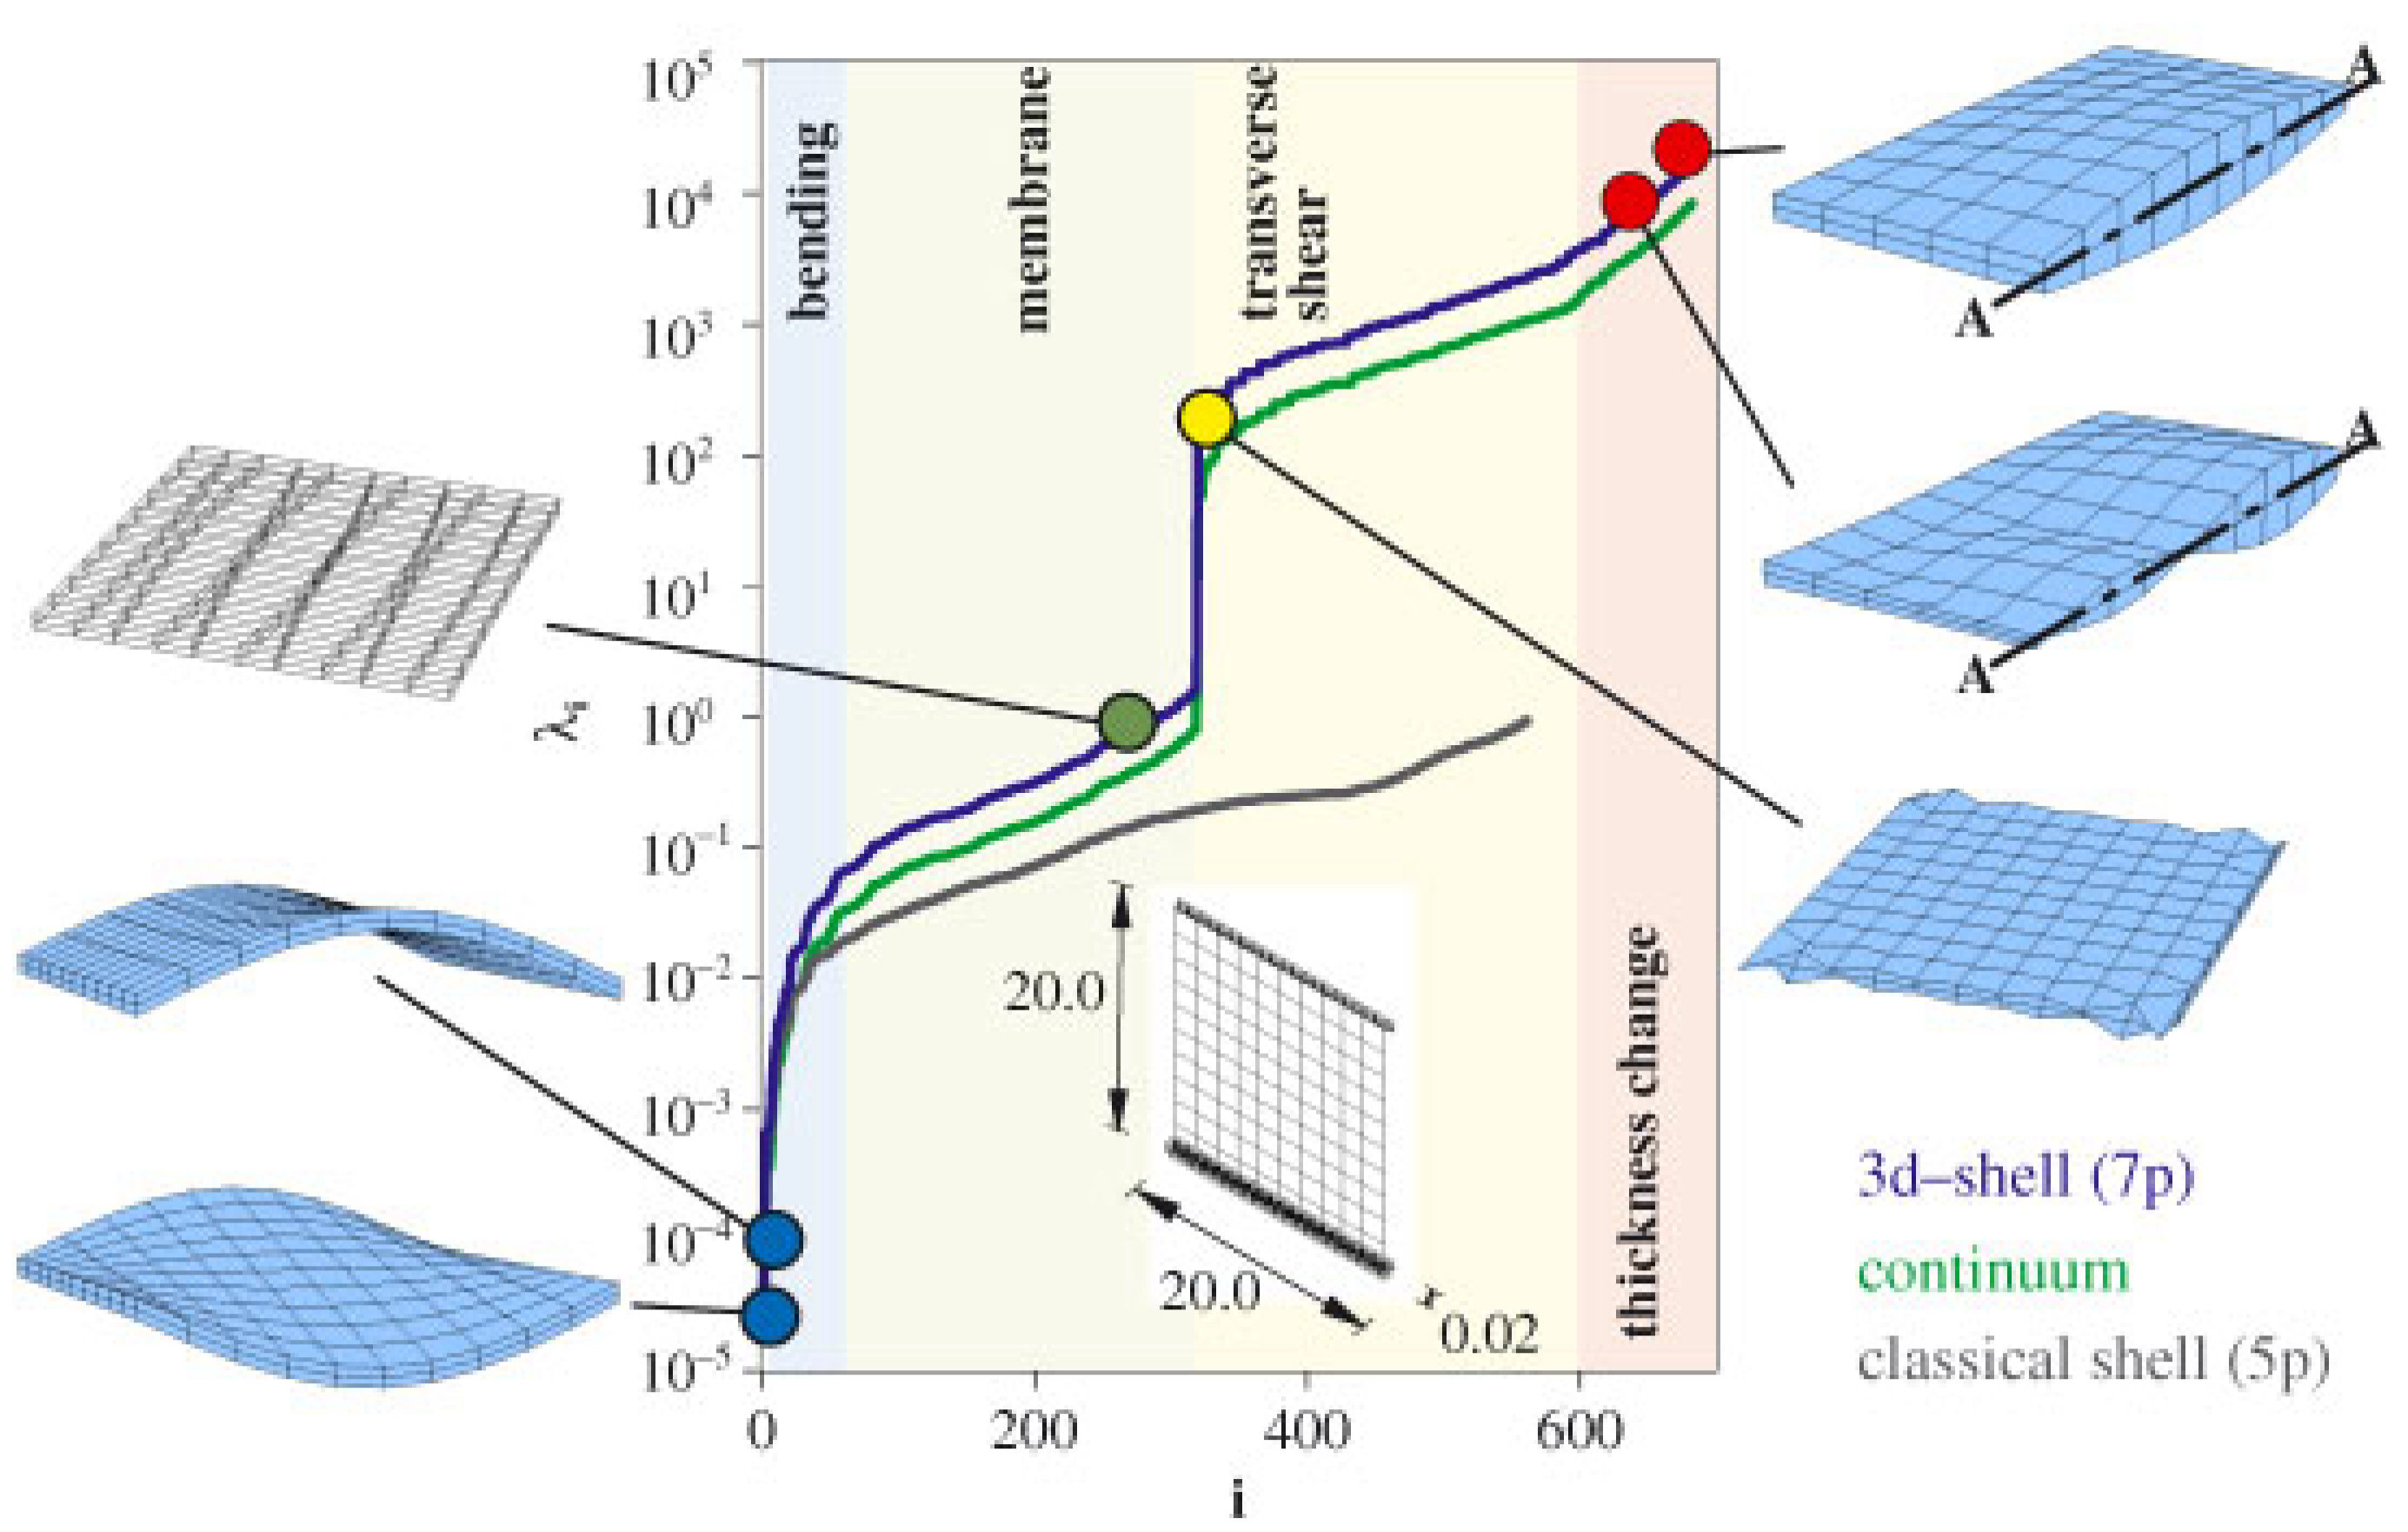
\includegraphics[width=12cm]{images/eigenvaluespectra.png}
	\caption{Eigenvalue spectra of various shell models \cite{RammLitBook04}}
	\label{shelleigenvaluespectra}
\end{figure}

As expected, the 7 parameter model captures higher Eigen-frequencies associated with thickness modes, while the 5 parameter is unable to resolve these. This is yet another example of model selection limiting the possibility of phenomena resolved.

\section{Locking in shell finite elements}

Surveying a range of shell models has confirmed that not all of them are appropriate for every type of analysis. One must consider the capabilities of the model in conjunction with the supposed critical phenomena of the analysis at hand. Thus, the analysis results are a function of physics the shell model can \textit{express}. This concept of expression limitation is vital to the correct understanding of shells in the FEM. If the isogeometric approach to the FEM is employed, the field of quantities in the problem are interpolated between discrete nodal values $\hat{(\ )}$ using shape functions $\mathbf{N}$. In general:

\singlespacing
\begin{equation} 
\begin{pmatrix}
\mathbf{R} \\
\mathbf{v} \\
\epsilon_{ij} \\
\vdots
\end{pmatrix}
(\xi,\eta)
=
\sum_{m=1}^{n\ nodes}
N(\xi,\eta)_m
{\begin{pmatrix}
	\hat{\mathbf{R}}_m \\
	\hat{\mathbf{v}}_m \\
	\hat{\epsilon_{ij}}_m \\
	\vdots
	\end{pmatrix}}
\label{eqfemtech1}
\end{equation}

\doublespacing

The resolving power of the shape functions undoubtedly restricts what continuous fields can be determined from discrete values. They govern not only the description of geometry, but also the deformation modes the element can express. This forms another layer of expression limitation added to shell models in FEM. Given the propensity to use linear or quadratic shape functions in modern FEM codes, these limitations are often not insignificant. These, together with the physics assumptions and limitations of each shell model, give rise to common numerical inaccuracies, generally termed locking.

\subsection{Transverse shear locking} \label{transverse_shear_locking}

Transverse shear locking is perhaps the most recognized and problematic locking phenomena amongst the three considered in this work. As it is related to transverse shear strains, transverse shear locking is possible  in the 5 parameter model and impossible for membrane and 3 parameter models. Phenomenologically, transverse shear locking occurs when thin shells incorrectly described by a 5 parameter model are subject to bending situations, with the signature of significantly reduced displacements (ie. 'locked') than expected. By indicating specific material matrices, and removing membrane work, the internal virtual work of the 5 parameter model is clarified: 

\singlespacing
\begin{equation} 
\bar{\mathbf{C}} =
\begin{pmatrix}
1 & \nu & 0 \\
\nu & 1 & 0 \\
0 & 0 & \frac{1-\nu}{2}
\end{pmatrix}
\hspace{10mm}
\mathbf{C}_{bend} = \frac{E t^3}{12(1-\nu^2)} \bar{ \mathbf{C}}
\hspace{10mm}
\mathbf{C}_{shear} = \alpha G t \mathbf{I}
\label{eqlock1}
\end{equation}

\begin{equation} 
-( \delta\Pi_{int} - \delta\Pi_{int\ mem} )=
-(\Pi_{bend} + \Pi_{shear}) =
\int_\Omega
\boldsymbol{\kappa}
:
\frac{E t^3}{12(1-\nu^2)} \bar{ \mathbf{C}}
:
\delta \boldsymbol{\kappa}\ 
d \Omega\ 
+
\int_\Omega
\boldsymbol{\gamma}
:
\alpha G t \mathbf{I}
:
\delta \boldsymbol{\gamma}\ 
d \Omega
\label{eqlock2}
\end{equation}

\doublespacing

As phenomenologically described, transverse shear locking comes into effect with thin shells. One can see that as $t \rightarrow 0$ the bending internal work ($\Pi_{bend} \propto t^3$) will be far less than the shear internal work ($\Pi_{shear} \propto t$), leading to an incorrect allocation of internal energy. Since the bending internal work is associated with bending deflections, these resulting deflections will be less than they should be and the element will appear locked. The over-representation of shear strains also leads to strong shear force oscillations - another classic symptom of transverse shear locking.


\subsection{Membrane locking}

Membrane locking is the inability to undergo inextensional bending deformations without parasitic membrane contributions. Physically, a primary symptom of this is significantly reduced deformations under pure bending action. Element curvature is a necessary condition for membrane locking, while increasing slenderness exacerbates the problem. Similar to transverse shear locking, as $t \rightarrow 0$ the bending internal work ($\Pi_{bend} \propto t^3$) reduces at a far greater rate than the membrane internal work ($\Pi_{mem} \propto t$) leading to artificial membrane contributions. Thus, membrane locking is possible in 3, 5, and 7 parameter models. The following figure illustrates the increasing severity of membrane locking as slenderness increases for 3 and 5 parameter NURBS based shell models.

\begin{figure}[H]
	\centering
	\def\svgwidth{\columnwidth}
	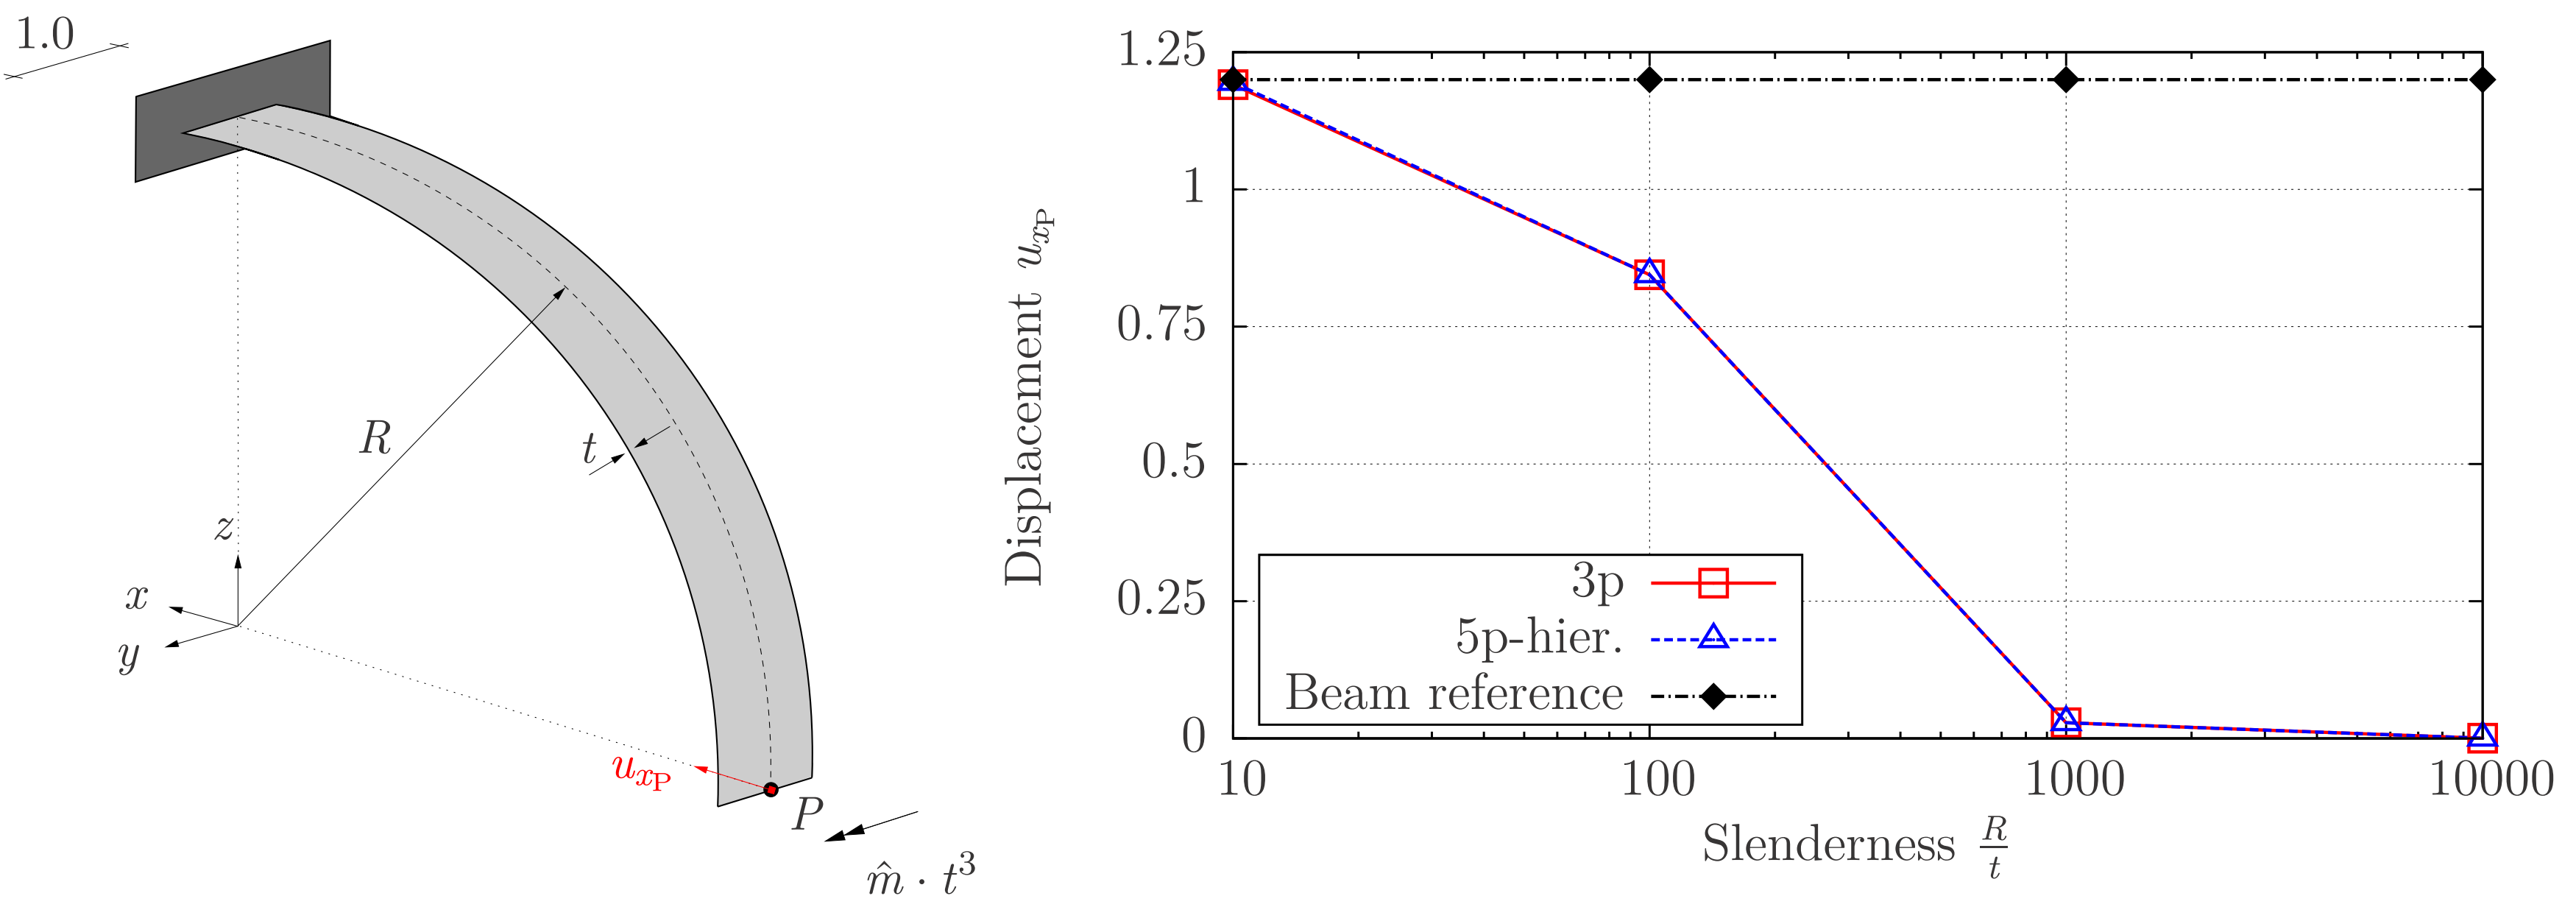
\includegraphics[width=14cm]{images/membranelocking.png}
	\caption{Convergence of cylindrical shell problem demonstrating membrane locking \cite{Echter13}}
	\label{ansexample}
\end{figure}

Despite the bleak results of the above problem, especially in high slenderness range, Bischoff et al. \cite{BischLitBook04} suggest that the adverse effects of membrane locking are mild when using bilinear shape functions, and completely ignored in linear triangle elements (where curvature is always zero). These lower order finite elements form the bulk of what used in commercial FEM codes and are the focus of this work.

\subsection{Curvature thickness locking}

Curvature locking is another locking consideration that only occurs in curved structures with 7 parameter models. The hallmark of curvature thickness locking is artificial through-thickness strains $\epsilon_{33}$ under pure bending action. Since the focus of this work is 3 and 5 parameter models that don't include normal strains $\epsilon_{33}$, the reader is referred to Bischoff et al. \cite{BischLitBook04} and Echter \cite{Echter13} for further information.





\section{Shell finite element technologies}

The previous discussion of locking phenomena associated with pure displacement formulations of shell finite elements has given rise to a number of shell finite element technologies to improve element performance. Broadly speaking, these mitigation approaches fall into two categories: reduced integration and B-Bar $\bar{\mathbf{B}}$ approaches which modify the strain displacement matrix $\mathbf{B}$. 

\subsection{Reduced integration}

One of the simplest and oldest methods of curbing locking is reduced integration, which deliberately uses less Gauss points than required to integrate the element stiffness matrix. Typically implemented as selective reduced integration (SRI), where the bending component is fully integrated and only the shear part undergoes reduced integration, the efficacy of the method relies on how susceptible the reduced integration Gaussian point locations are to parasitic strains. Despite this chance aspect, it is often used in crash worthiness simulations with the benefits of reduced locking and reduced computational time. The following graph compares the performance (scaled displacement vs. slenderness) of a fully and reduced integrated 5 parameter shell against the reference solution for a square plate in bending.

\begin{figure}[H]
	\centering
	\def\svgwidth{\columnwidth}
	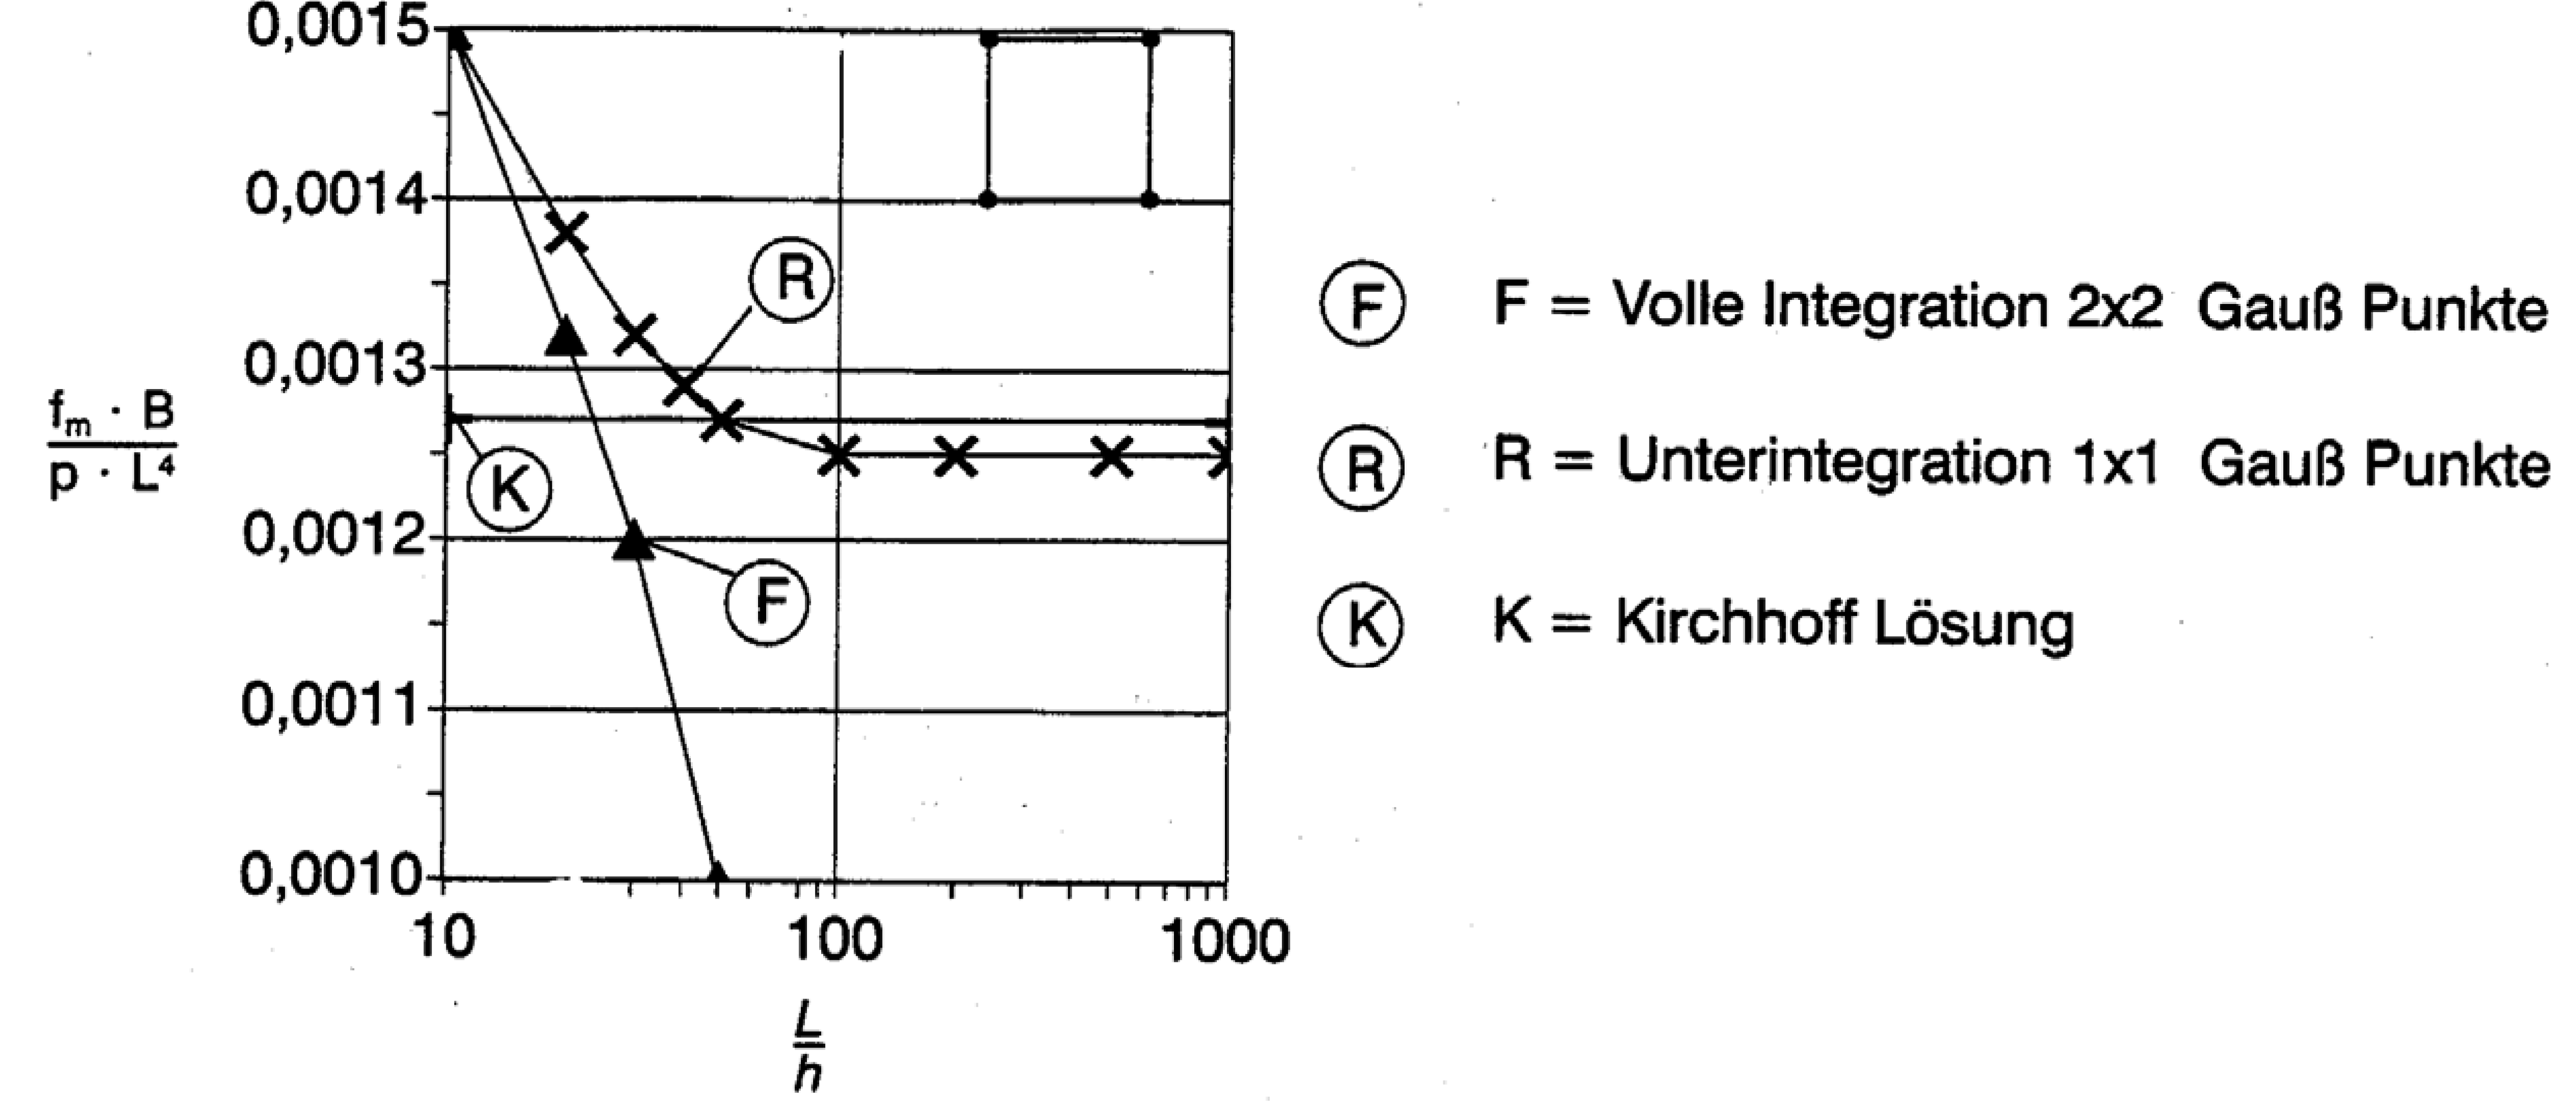
\includegraphics[width=14cm]{images/shearlockingredint.png}
	\caption{Reduced integration of a 5 parameter Quad 4 shell \cite{Bletz16}}
	\textit{F = Full integration, R = Reduced integration, K = Kirchhoff (3 parameter model) solution}
	\label{shearlockingredint}
\end{figure}

It's clear that the normal fully integrated element exhibits severe locking, while the element with reduced integration converges to a value close to the reference solution. Despite this, SRI in general still doesn't guarantee complete removal of shear locking and also introduces spurious zero energy modes. These zero energy modes are often combated by stabilizing matrices ("hourglass" control \cite{Zien2Vol2000}) which are designed to be activated under the spurious zero-energy regimes and noted as quite complex to formulate \cite{Mohan97}. An additional drawback of reduced integration is element performance deterioration as the mesh becomes distorted and warped \cite{Nguyen2009} \cite{Yang2000}.

\subsection{Assumed Natural Strains}

The Assumed Natural Strain (ANS) approach forms a main umbrella of B-Bar methods, which alters the strain-displacement matrix $\mathbf{B}$ to mitigate locking. The ANS approach \cite{MACNEAL1982} works by computing the strain values at particular co-location points less susceptible to parasitic strains in the element (normally chosen as mid-edge and/or centre points) and then interpolating these discrete values through the element to define a new "assumed" shear strain field. As a general approach, many subsequent technologies fall under the ANS umbrella.

\subsection{Mixed Interpolation of Tensorial Components}

Falling within the ANS framework, Dvorkin and Bathe \cite{Dvorkin84} \cite{Bathe86} developed the Mixed Interpolation of Tensorial Components (MITC) approach which relies on an assumed shear strain field. A graphical example of this formulation is demonstrated below on a Quad 4 element, with linear interpolation of the shear strain field at mid-side points.

\begin{figure}[H]
	\centering
	\def\svgwidth{\columnwidth}
	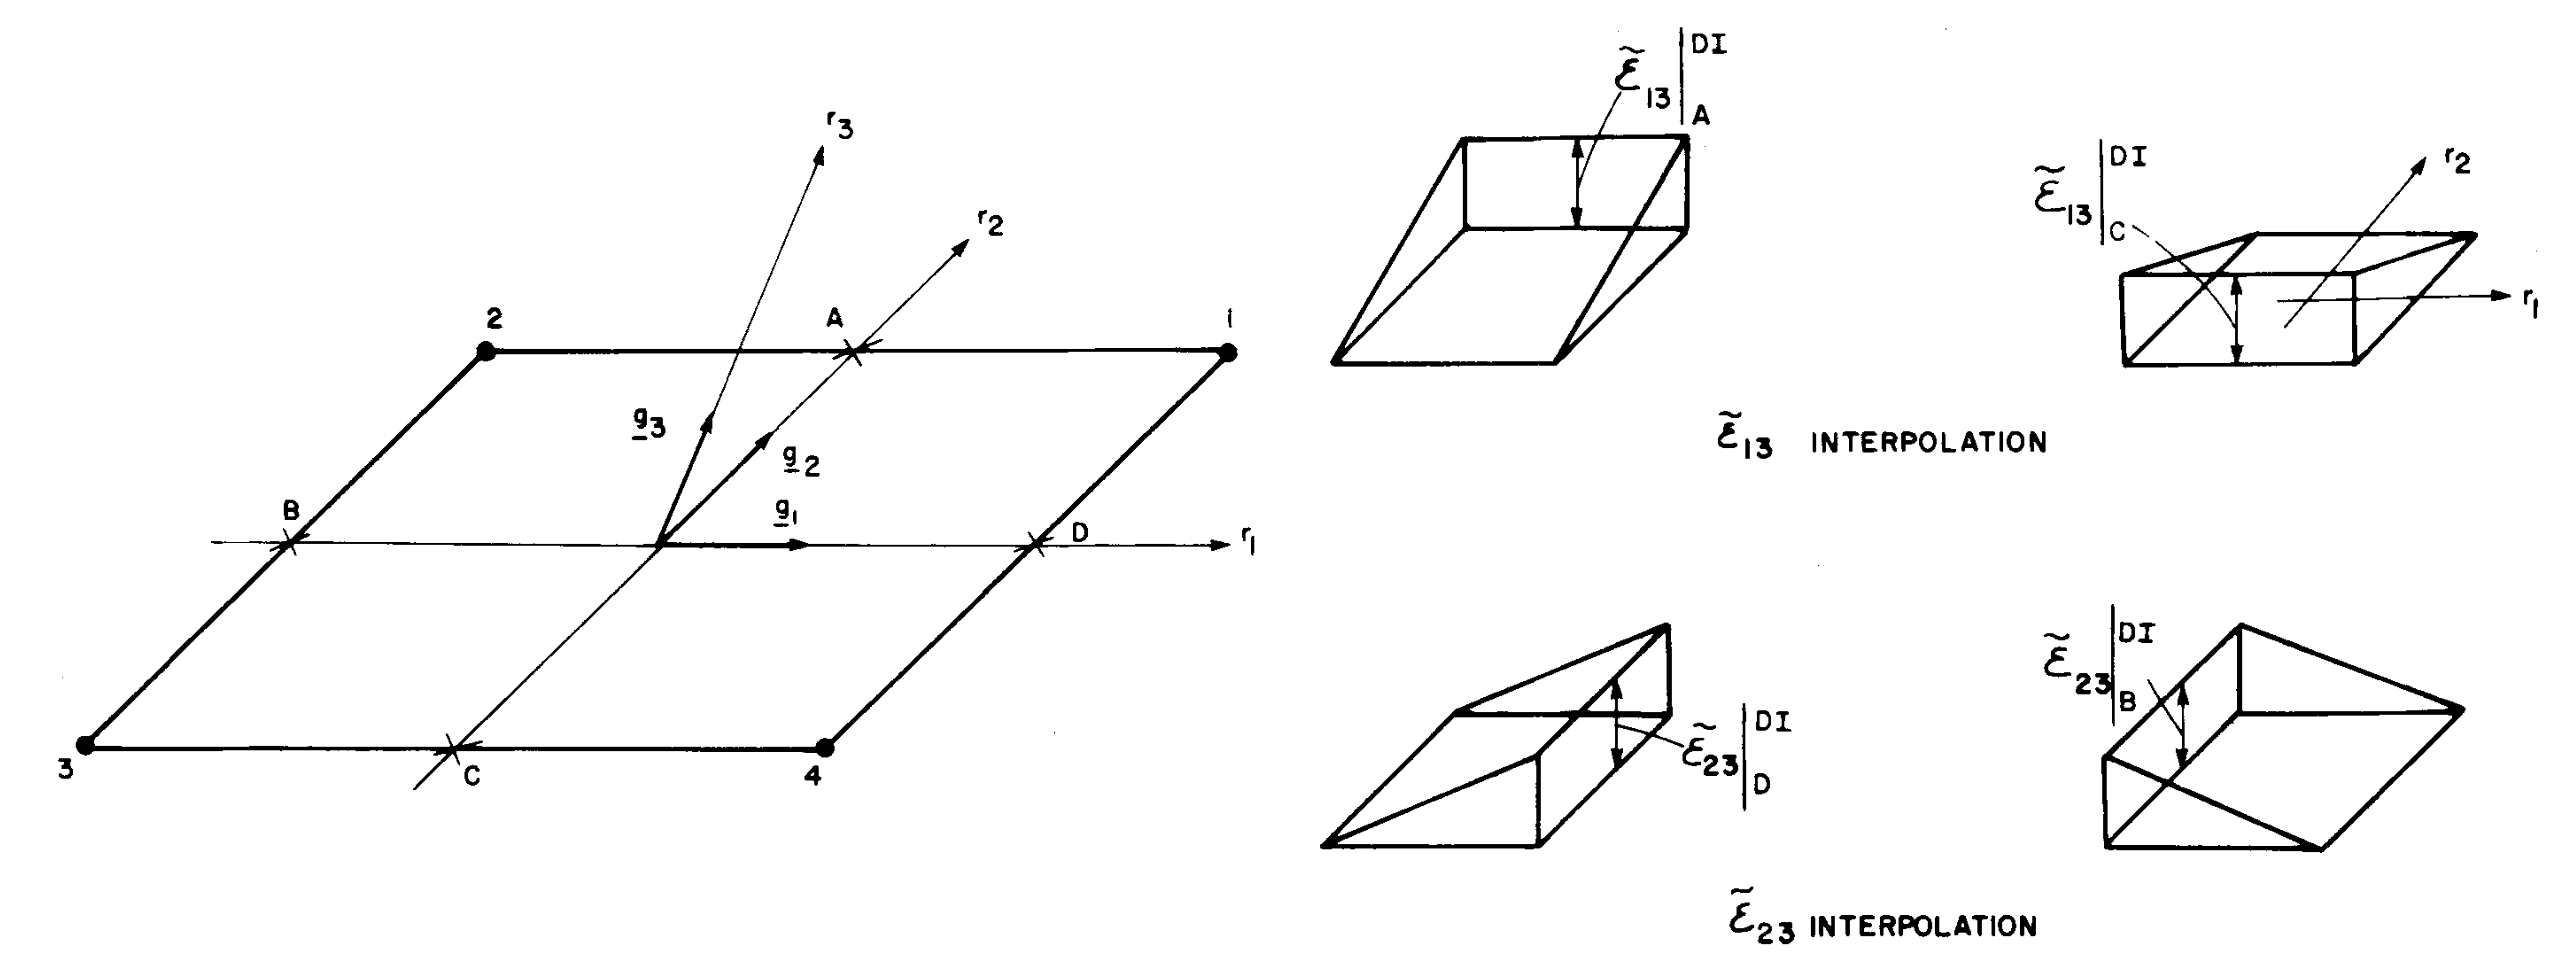
\includegraphics[width=16cm]{images/mitc4.png}
	\caption{Assumed shear strain field of the MITC4 element \cite{Bathe86}}
	\label{ansexample}
\end{figure}

The performance of the MITC formulation clearly depends on the location of the sampling points, and their susceptibility to parasitic shear strains under the case considered. Despite this, the MITC elements have proven resistant to membrane and transverse shear locking \cite{Bathe86} and are amongst the most widely used elements throughout FEM codes.

\subsection{Assumed Natural Deviatoric Strains}

The ANS approach was extended into Free Formulation (FF) \cite{Bergan84}, where the element stiffness matrix is the sum of a basic and higher order stiffness, by Militello and Felippa \cite{FELIPPA1990} under the name of the Assumed Natural Deviatoric Strains (ANDES) formulation. An advantage that the ANDES formulation inherits from the FF is that it untethers the derivation of element stiffness from the principle of minimum potential energy, the function continuity requirements of which often result in elements that "tend to be too stiff" \cite{Bergan84}. The ANDES basic stiffness ensures consistency of the element and arrises from the basic strain field comprising constant strain states and those associated with rigid body motion. Complementing this, the higher order stiffness is responsible for stability and accuracy \cite{Felippa2003} based on a enhanced strain field where the element enhancements are realised. The FF framework requires this potentially non-conforming higher order field be energy orthogonal to the basic field, which the ANDES formulation fulfils with a deviatoric higher order strain field \cite{felippa2002fitting}.  The ANDES formulation has proven capable of alleviating membrane and transverse shear locking \cite{Mostafa11}.

\subsection{Discrete Shear Gap}

The Discrete Shear Gap (DSG) approach from Bischoff and Bletzinger \cite{Ble00} \cite{Bis04} is another variant on the ANS approach with the novelty of identifying and manipulating the 'shear gap' field of the element. The shear gap, as illustrated below, is the increase of displacement due to shear, and corresponds to the difference between the actual displacement and that of pure bending (thus the shear gap is always zero in a 3 parameter Kirchhoff-Love model).

\begin{figure}[H]
	\centering
	\def\svgwidth{\columnwidth}
	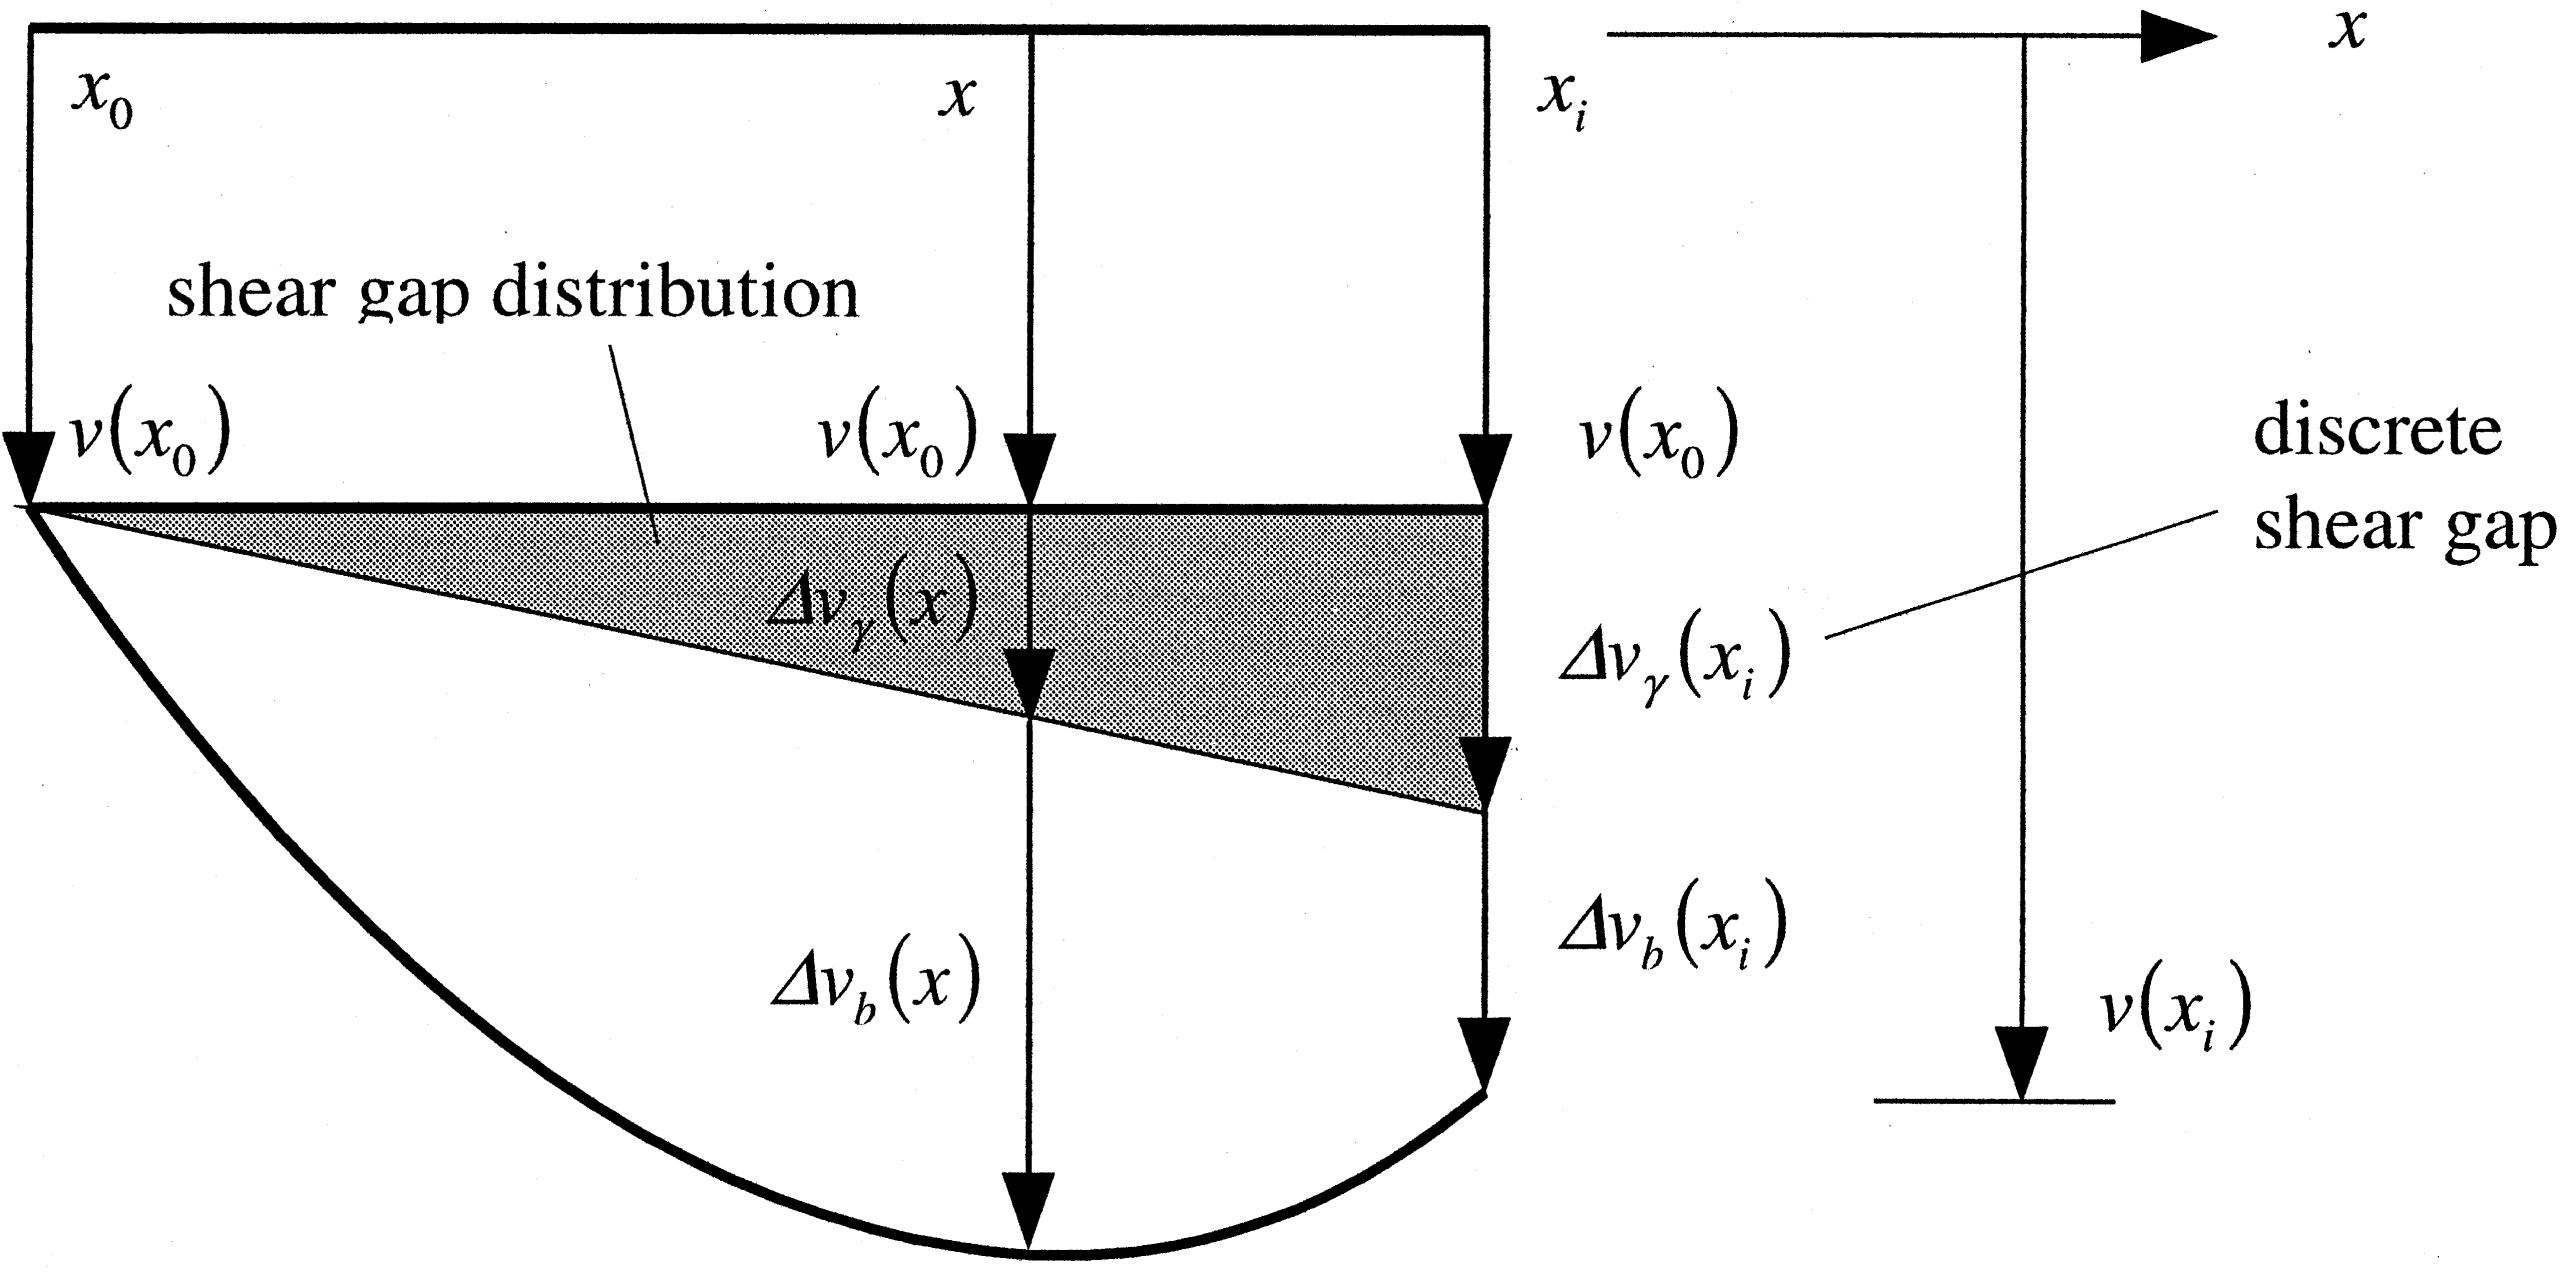
\includegraphics[width=8cm]{images/DSG.png}
	\caption{Discrete Shear Gap (DSG) concept \cite{Ble00}}
	\label{ansexample}
\end{figure}

The DSG method aims to set the nodal shear gaps to zero, which, in effect, alters and defines the underlying shear strain field. In bilinear rectangular applications of the DSG method, Bletzinger \cite{Ble00} notes that the MITC4 element is recovered. For a linear triangle element, the shear gap of only two nodes can be set to zero, rendering the element stiffness dependent on node ordering \cite{Ble00}. Despite this drawback, which diminishes with mesh refinement, the DSG method offers an advantage of very fast computational construction of element stiffness matrices and effective mitigation of transverse shear locking.

\subsection{Discrete Kirchhoff Theory}

Elements based on the Discrete Kirchhoff Theory (DKT) are obtained by modifying a basic 5 parameter element and ignoring the transverse shear energy \cite{Batoz1980}. Since the underlying kinematics of the 5 parameter model are different to Kirchhoff bending theory, the Kirchhoff constraints are enforced via discrete points (typically nodes and mid-edge points) along the element edges relating the rotations to translational displacements. The geometry and tying-points of the Discrete Kirchhoff Quadrilateral (DKQ) element are shown below:

\begin{figure}[H]
	\centering
	\def\svgwidth{\columnwidth}
	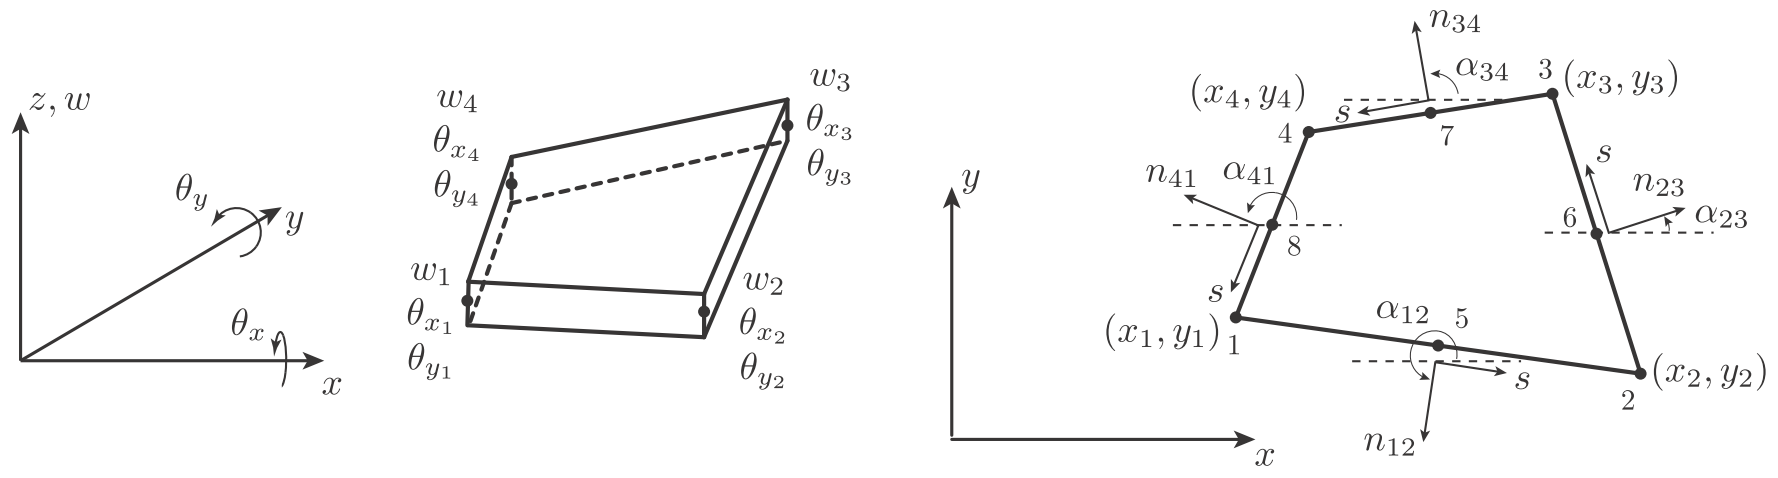
\includegraphics[width=15cm]{images/8nodeseren.png}
	\caption{DKQ DOF arrangement and geometry \cite{Bar12}}
	\label{DKQlayout}
\end{figure}

For example, the Kirchhoff conditions are imposed at corner nodes $i = 1, 2, 3, 4$ and mid-side nodes $k = 5, 6, 7, 8$ \cite{Bar12}:

\begin{equation} 
\beta_{xi} + \frac{\partial w}{\partial x} \rvert_i = 0\ ,
\hspace{10mm}
\beta_{yi} + \frac{\partial w}{\partial y} \rvert_i = 0\ ,
\hspace{10mm}
\beta_{sk} + \frac{\partial w}{\partial s} \rvert_k = 0
\label{eqsdkt}
\end{equation}

Mohan \cite{Mohan97} noted that a major drawback of DKT elements is that the transverse displacement isn't explicitly defined within the interior of the element. Despite this, the advantages of DKT formulated elements is that they combine the shear locking free performance of KL models and the lower $C_0$ continuity requirements of RM models \cite{Bletz16}.

\subsection{Enhanced Assumed Strains}

The Enhanced Assumed Strain (EAS) approach \cite{Simo1990} utilises the three field Hu-Washizu variational principle which allows the simultaneous variation of displacements, stresses and strains. Unlike the other technologies presented which attempt to remove problematic strain terms associated with locking, EAS derived elements feature additional enhanced strain fields designed to balance the parasitic displacement based strain terms. To prevent singular matrices the enhanced strains must be linearly independent from the displacement based strains. Furthermore, orthogonality of the stress functions to the enhanced strains must be ensured such that the associated energy vanish \cite{Echter13}. The application of EAS techniques to elements has been found to improve transverse shear and membrane locking performance \cite{Simo1990} \cite{BischLitBook04} \cite{Echter13}.

\subsection{Drilling degrees of freedom}

Although drilling degrees of freedom (DOFs) don't counter locking problems, it is a commonly employed finite element technique. The common analysis of structural connections and custom steelwork are instances where shell elements will intersect with each other at arbitrary orientations. The discussion of 3 and 5 parameter shell models confirmed the nodal DOFs to be 3 translation and 2 rotational components:

\begin{equation} 
\mathbf{v}_i^T = \begin{pmatrix}
v_{xi} & v_{yi} & v_{zi} & \beta_{xi} & \beta_{yi}
\end{pmatrix}
\label{eqsdrilling}
\end{equation}

It can be seen that the shell formulations don't require a rotational DOF around the z axis $\beta_{zi}$, referred to as the drilling DOF. However, as discussed, shell elements in practical FEA may meet at arbitrary orientations, such as the perpendicular intersection below:

\begin{figure}[H]
	\centering
	\def\svgwidth{\columnwidth}
	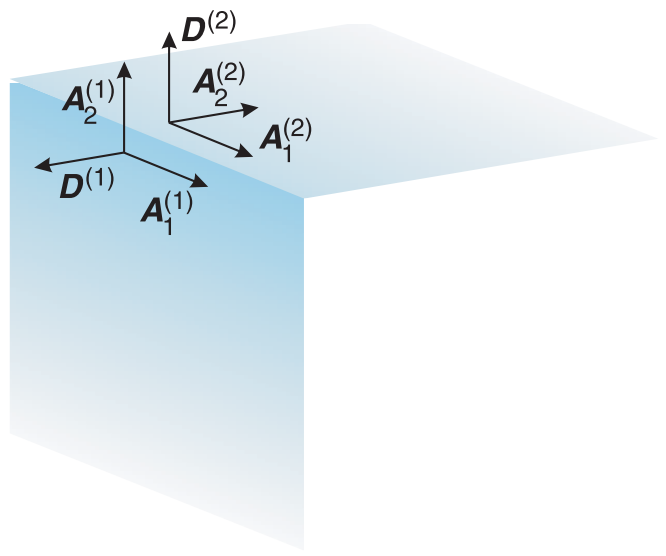
\includegraphics[width=8cm]{images/drillingDOF.png}
	\caption{Shell assembly benefitting from drilling DOFs \cite{BischLitBook04}}
	\label{shellModels}
\end{figure}

The figure above illustrates that the real twisting DOF associated with $A_2^{(2)}$ mates with the drilling DOF associated with $D^{(1)}$, which has no theoretically based stiffness value according to the shell formulations. In the current arrangement the connection will clearly be modelled too flexibly.  A remedy for this is the addition of an artificial drilling DOF stiffness to the element, however the magnitude of such a fictitious torsional spring has no decisive theoretical foundation. Intuitively, it should be done on an element by element basis and should vary with the characteristic size and stiffness of the element, as opposed to a global constant drilling stiffness. Among others available, one common technique is to introduce a scaling factor (in the strain-displacement matrix or after the element stiffness matrix is constructed) which takes a fraction of the element stiffness and assigns it to the drilling DOFs. 

\subsection{Summary of selected element technologies}

Following the discussion of shell models, their associated locking phenomena and element technologies, a summary of the element technologies considered with their relative merits and drawbacks is tabulated below:

\begin{table}[H]
	\begin{tabularx}{\textwidth}{ | l | l |  X | X | }
		\hline
		\textbf{Technology} 		& 	\textbf{Formulation}	&		\textbf{Advantages}	&		\textbf{Disadvantages}\\
		\hline
		ANDES	& 5 parameter &	Reduced membrane and transverse shear locking &  Locking reduction depends on tying points \\
		\ &\  & Relaxed higher order strain field & More complex implementation \\
		\hline
		ANS & 5 parameter		&  Reduced membrane and transverse shear locking & Locking reduction depends on tying points \\
		\hline
		DKT	&  3 parameter		 & 	No transverse shear locking & Transverse disp. not explicitly defined \\
		\hline
		Drilling DOFs	  &  - & Practical assembly of shells & Artificial stiffness \\
		\hline
		DSG	&	 5 parameter	& Reduced transverse shear locking	& Node numbering dependency for linear triangle \\
		\ &\  & Computationally fast & \  \\
		\hline
		EAS 	  &		  5 parameter		&		Reduced transverse shear and membrane locking & Potentially complex implementation and possibly slower \\
		\hline
		MITC	&		5 parameter	&		Reduced membrane and transverse shear locking & Locking reduction depends on tying points \\
		\hline
		Reduced &		-		&	 Lowered computational cost & Zero energy modes \\
		integration &\  & Reduced locking & Locking reduction depends on integration points \\ 
		\hline
	\end{tabularx}
	\caption{Summary of selected element technologies}
	\label{table:1}
\end{table}

The table above confirms the \textit{"no free lunch"} theory, with every technology having its own advantages and drawbacks. In the case of a flat shell (naturally, or via projection), where the bending and membrane response are decoupled, a single finite element can easily employ different technologies in each component. 

\section{Identification of KRATOS shell element formulations}

The shell elements to be implemented in KRATOS are the 5 parameter (Reissner-Mindlin theory) triangular shell and the 3 parameter (Kirchhoff Love theory) quadrilateral shell. Obviously the perfect element choices for KRATOS would be computationally quick, possess no locking and easy to implement, but it's clear such an element doesn't exist yet. If the requirements are relaxed to computationally quick elements that are relatively free of locking effects the following candidates are selected:

\begin{table}[H]
	\begin{tabularx}{\textwidth}{ | l | X |  X | }
		\hline
		\textbf{Element} 		& 	\textbf{Membrane formulation}	&		\textbf{Bending formulation}	\\
		\hline
		Thick triangular shell
		&
		DSG + Drilling DOFs
		&
		DSG \\
		\hline
		Thin quadrilateral shell
		&
		ANDES including Drilling DOFs
		&
		DKT \\
		\hline
	\end{tabularx}
	\caption{Selected formulations of implemented shell elements}
	\label{table:2}
\end{table}

With the various components of the KRATOS shell elements selected, they shall be implemented in the following sections of this work, commencing with the DSG triangular element.
 %shells
%%%%%%%%%%%%%%%%%%%%%%%%%%%%%%%%%%%%%%%%%%%%%%%%%%%%%%%%
%%%%                                              %%%%%%
%%%%  Author: Peter Wilson                        %%%%%%
%%%%                                              %%%%%%
%%%%  DSG triangle element                        %%%%%%
%%%%                                              %%%%%%
%%%%%%%%%%%%%%%%%%%%%%%%%%%%%%%%%%%%%%%%%%%%%%%%%%%%%%%%


%fref generates automatically the respective abreviation/word in the text for the reference. You just have to define a label starting with the respective keyword.
%english: chap, sec, fig, eq, app
%deutsch: chap/kap, abs, abb, gl, anh
%see http://ctan.space-pro.be/tex-archive/macros/latex/contrib/fancyref/fancyref.pdf for more information




\setcounter{MaxMatrixCols}{20}

%\abovedisplayskip=5pt

%\setlength{\belowdisplayskip}{-10pt}

%\setlength{\abovedisplayskip}{-10pt}
%\belowdisplayskip=5pt

\chapter{DSG triangle shell element}
\label{chap:chapter_3}

\renewcommand{\Thema}{DSG triangle shell element}

The follow sequence elucidates the formulation and implementation of the stiffness matrix, mass matrix and quantity recovery associated with the DSG triangle shell element in Kratos. 

\section{Stiffness matrix formulation}

Based on the 5 parameter Reissner-Mindlin shell theory, the thick shell considers internal energy contributions from membrane, bending and shear components. As discussed in Chapter \ref{chap:chapter_2}, basic finite elements derived from this shell theory face locking problems as the shell slenderness ratio increases. The element implemented is Bletzinger's Discrete Shear Gap (DSG) shell \cite{Ble00} which incorporates an enhanced shear strain formulation to mitigate the aforementioned locking. This triangular element has 18 DOFs ordered as such:
\begin{equation} 
\mathbf{u}^T = 
\begin{pmatrix}
\mathbf{u_1} & \mathbf{u_2} & \mathbf{u_3}
\end{pmatrix} 
\hspace{10mm}
where
\hspace{10mm}
\mathbf{u}_i^T = 
\begin{pmatrix}
{u_{xi}} & {u_{yi}} & {u_{yi}} & {\beta_{xi}} & {\beta_{yi}} & {\beta_{zi}}
\end{pmatrix}
\label{eqt1}
\end{equation}
The element displacement field is related to the discrete nodal values via shape functions.
\begin{equation} 
\mathbf{u}(x, y) = \sum_{i=1}^3 \ N_i(x,y) \mathbf{u}_i
\label{eqt2}
\end{equation}
$N_i$ are the standard linear triangle shape functions, referred to the Cartesian system, considering the corner points of the triangle $x_i,\ y_i$.
\begin{gather} 
	\begin{aligned}
		&N_1 (x , y) = \frac{1}{2 A} \big[ (x_2 y_3 - x_3 y_2) + x(y_2 - y_3) + y(x_3 - x_2) \big]
		\\
		&N_2 (x , y) = \frac{1}{2 A} \big[ (x_3 y_1 - x_1 y_3) + x(y_3 - y_1) + y(x_1 - x_3) \big]
		\\
		&N_3 (x , y) = \frac{1}{2 A} \big[ (x_1 y_2 - x_2 y_1) + x(y_1 - y_2) + y(x_2 - x_1) \big]
		\label{eqt3}
	\end{aligned}
\end{gather}

Analogous to internal energy, the element stiffness matrix of the DSG triangle can be decomposed into membrane, bending and shear contributions.

\begin{equation} 
\mathbf{K} = \mathbf{K}_{mem} + \mathbf{K}_{bend} + \mathbf{K}_{shear}
\label{eqt4}
\end{equation}

The above expression can be expanded into strain-displacement and material matrices relevant for each component.

\begin{equation} 
\mathbf{K} = \int_A  (\mathbf{B}_{mem}^T \mathbf{C}_{mem} \mathbf{B}_{mem} + \mathbf{B}_{bend}^T \mathbf{C}_{bend} \mathbf{B}_{bend} + \mathbf{B}_{shear}^T \mathbf{C}_{shear} \mathbf{B}_{shear})\ dA
\label{eqt5}
\end{equation}

Rama et al. \cite{Ram16} present the DSG formulation in a similar manner, detailing the strain displacement matrix and material material of each constituent separately.

The membrane strain displacement matrix requires no enhancement since linear triangle elements are impervious to membrane locking as discussed in section \ref{membrane_locking_theory}. Thus, the standard displacement-based formulation can be confidently utilised:

\begin{equation}
\boldsymbol{\epsilon} =(\nabla \mathbf{N}^{u_{i}}) \hat{\mathbf{v}} 
= \mathbf{B}_{mem} \hat{\mathbf{v}}  
\label{eqt5_1}\ .
\end{equation}

Clarifying $\mathbf{B}_{mem}$ yields:

\begin{equation} 
\mathbf{B}_{mem} =  \begin{pmatrix}
\mathbf{B}_{mem_1} & \mathbf{B}_{mem_2} & \mathbf{B}_{mem_3}
\end{pmatrix} 
\label{eqt6}\ ,
\end{equation}

and with increased resolution:

\begin{equation} 
\mathbf{B}_{mem_i} =  \begin{pmatrix}
N_{i,x} & 0 & 0 & 0 & 0 & 0 \\
0 & N_{i,y} & 0 & 0 & 0 & 0 \\
N_{i,y} & N_{i,x} & 0 & 0 & 0 & 0 \\
\end{pmatrix} 
\label{eqt7}\ .
\end{equation}

The bending strain displacement matrix is also a simple standard displacement-based formulation and can be presented in a similar manner:

\begin{equation}
\boldsymbol{\kappa} =(\nabla \mathbf{N}^{\theta_{i}}) \hat{\mathbf{v}} 
= \mathbf{B}_{bend} \hat{\mathbf{v}}  
\label{eqt7_1}\ .
\end{equation}

Clarifying $\mathbf{B}_{bend}$ yields:

\begin{equation} 
\mathbf{B}_{bend} =  \begin{pmatrix}
\mathbf{B}_{bend_1} & \mathbf{B}_{bend_2} & \mathbf{B}_{bend_3}
\end{pmatrix} 
\label{eqt8}\ ,
\end{equation}

with individual entries detailed as:

\begin{equation} 
\mathbf{B}_{bend_i} =  \begin{pmatrix}
0 & 0 & 0 & 0 & N_{i,x} & 0 \\
0 & 0 & 0 & -N_{i,y} & 0 & 0 \\
0 & 0 & 0 & -N_{i,x} & N_{i,y} & 0
\end{pmatrix} 
\label{eqt9}\ .
\end{equation}

Finally, the shear strain displacement matrix, which implements the DSG element enhancement technology fully derived in Appendix \ref{app:DSG technology derivation} and mitigates shear locking, is summarily expressed as follows:

\begin{gather} 
	\begin{aligned}
		& \mathbf{B}_{shear} =  \frac{1}{2 A}
		\begin{pmatrix}
			0 & 0 & b-c & 0 & A & 0 & 0 & 0 & c & \frac{-bc}{2} & \frac{ac}{2} & 0 & 0 & 0 & -b & \frac{bc}{2} & \frac{bd}{2} & 0 \\
			0 & 0 & d-a & -A & 0 & 0 & 0 & 0 & -d & \frac{bd}{2} & \frac{-ad}{2} & 0 & 0 & 0 & a & \frac{-ac}{2} & \frac{ad}{2} & 0
		\end{pmatrix}
		\\
		& with:\ 
		a = x_2-x_1,\ 
		b = y_2-y_1,\ 
		c = y_3-y_1,\ 
		d = x_3 - x_1
		\label{eqt10}
	\end{aligned}
\end{gather}

The standard isotropic material matrices for the membrane and bending components are presented below:

\begin{equation} 
\mathbf{C}_{mem} =  \frac{Eh}{(1-\nu^2)}
\begin{pmatrix}
1 & \nu & 0 \\
\nu & 1 & 0 \\
0 & 0 & \frac{(1-\nu)}{2}
\end{pmatrix}
\label{eqt11}\ ,
\end{equation}

\begin{equation} 
\mathbf{C}_{bend} =  \frac{E h^3}{12(1-\nu^2)}
\begin{pmatrix}
1 & \nu & 0 \\
\nu & 1 & 0 \\
0 & 0 & \frac{(1-\nu)}{2}
\end{pmatrix}
\label{eqt12}\ .
\end{equation}

To further improve the DSG element performance, Bischoff and Bletzinger \cite{Bis04} \cite{Bis01} applied the enhancement approach that Lyly suggested for MITC-4 elements \cite{Lyl93}. This approach modifies the internal shear energy term by scaling the shear constitutive matrix with a correction term $\tau$ incorporating the element thickness and an indicator of element size ($h_k$ = longest element side length). The enhanced  shear constitutive matrix is thus:

\begin{equation} 
\mathbf{C}_{shear} =  \tau \kappa Gh
\begin{pmatrix}
1 & \nu \\
\nu & 1 
\end{pmatrix}
=
\frac{\kappa G h^3}{h^2 + \alpha h_k^2}
\begin{pmatrix}
1 & \nu \\
\nu & 1 
\end{pmatrix}
\label{eqt14}
\end{equation}

where $\kappa = \frac{5}{6}$ is the shear correction factor and $\alpha = 0.1$ as per \cite{Lyl93}.

As described in section \ref{transverse_shear_locking}, transverse shear locking is driven by a mismatch of internal energy allocation between bending ($\Pi_{bend} \propto h^3$) and shear components ($\Pi_{shear} \propto h$) as $h \rightarrow 0$.  This modification somewhat alleviates the locking by 'encouraging' the internal shear energy to scale with the cube of the thickness too, thus reducing the artificial energy disparity.

Although all stiffness components are assembled, one notices that lack of entries corresponding to the drilling DOF $\beta_{zi}$ currently renders the element stiffness matrix singular. The technology of drilling DOFs discussed in \ref{drilling_DOF_section} in thus introduced. Nguyen-Thoi et al. \cite{Ngu13} proposed to remedy this rotational singularity by setting the drilling DOF entries to one one-thousandth of the maximum diagonal entry in the element stiffness matrix.

\begin{equation} 
K_{\beta_{zi}} =  \frac{max(K_{ij}\delta_{ij})}{1000}
\label{eqtdrilling}
\end{equation}

\section{Stiffness matrix implementation}
Despite the relatively simple decoupled stiffness formulation presented, the practical programming of it invariably introduces it's own complexities. Furthermore, leveraging the existing functionality that the Kratos code possesses not only prevents re-inventing the wheel, but also makes the code more readable and functionally cohesive.  

The new DSG triangle element is implemented in the files $\texttt{shell\_thick\_element\_3D3N.hpp}$ and $\texttt{shell\_thick\_element\_3D3N.cpp}$, which are compiled into the  'StructuralMechanicsApplication' module of Kratos. Without extending into extraneous details, the DSG triangle element is derived from the Kratos $\texttt{element}$ class and makes extensive use of other existing Kratos utility classes including those offering: coordinate transformations, material properties and pre-defined stiffness matrix and residual vector data types. Correspondingly, it is also subject to the constraints associated with each of these. From a high level view, however, the element stiffness matrix follows the subsequent workflow:

\begin{figure}[H]
	% Define block styles
	\tikzstyle{virtual} = [rectangle, minimum width=3cm, minimum height=1cm, text centered, draw=black, fill=orange!30]
	\tikzstyle{process} = [rectangle, minimum width=3cm, minimum height=1cm, text centered, draw=black, fill=white!30]
	\tikzstyle{arrow} = [thick,->,>=stealth]
	\begin{tikzpicture}[node distance = 1.9cm, auto]
	% Place nodes
	\node [process] (CalculateLocalSystem) {$\texttt{CalculateLocalSystem()}$};
	\node [process, right of=CalculateLocalSystem, xshift = 4cm] (CalculateAll) {$\texttt{CalculateAll()}$};
	\node [process, below of=CalculateAll, xshift = -0cm] (InitializeCalculationData) {$\texttt{InitializeCalculationData()}$};
	\node [process, below of=InitializeCalculationData, yshift = -0cm] (CalculateSectionResponse) {$\texttt{CalculateSectionResponse()}$};
	\node [process, below of=CalculateSectionResponse, yshift = -0cm] (FinalizeCalculations) {$\texttt{FinalizeCalculations()}$};
	% Draw edges
	\draw [arrow] (CalculateLocalSystem) -- (CalculateAll);
	\draw [arrow] (CalculateAll) -- (InitializeCalculationData);
	\draw [arrow] (InitializeCalculationData) -- (CalculateSectionResponse);
	\draw [arrow] (CalculateSectionResponse) -- (FinalizeCalculations);
	\end{tikzpicture}
	\caption{High level overview of DSG element workflow}
	\label{DSGworkflow}
\end{figure}

Initially, the re-implemented virtual method $\texttt{CalculateLocalSystem()}$ is called by the Kratos framework automatically for every $\texttt{ShellThickElement3D3N}$ in the job definition. This method redirects to $\texttt{CalculateAll()}$, which is the main pipeline of the element stiffness calculation, itself calling three key methods: $\texttt{InitializeCalculationData()},$ \break$\texttt{CalculateSectionResponse()}$ and $\texttt{FinalizeCalculations()}$.

Following the general form of the existing shell elements in Kratos, all the data which remains constant through the Gauss Integration loop is calculated beforehand in the function $\texttt{InitializeCalculationData()}$. The DSG element follows this tradition for consistency, although it isn't strictly necessary because it only requires one Gauss point for the numerical integration. Following $\texttt{InitializeCalculationData()}$, $\texttt{CalculateSectionResponse()}$ is called and the material matrix is populated with existing Kratos material classes. It must be noted here that a single 8$\times$8 material matrix $\mathbf{C}$ is returned which is structured as follows (for the setting of 'thick' shell kinematics):

\begin{equation} 
\mathbf{C}_{Kratos} =  
\begin{pmatrix}
	\mathbf{C}_{mem} & \mathbf{0} & \mathbf{0} \\
	\mathbf{0} & \mathbf{C}_{bend} & \mathbf{0} \\
	\mathbf{0} & 	\mathbf{0} & \mathbf{C}_{shear}
\end{pmatrix}
\label{eqtCkratos}
\end{equation} 

At this stage the shear component of the material matrix is currently unmodified, thus it is subsequently corrected with $\tau$ as per equation \eqref{eqt14}. The DOF arrangement of the material matrix also motivates a slight departure from the strain displacement matrices as presented above. Although the element stiffness matrix can certainly be programmed in it's constitutive parts, as per equation \eqref{eqt5}, it is more concise to calculate it as follows:

\begin{equation} 
\mathbf{K} = \int_A  (\mathbf{B}_{comb}^T \mathbf{C}_{Kratos} \mathbf{B}_{comb} )\ dA
= A\  \mathbf{B}_{comb}^T \mathbf{C}_{Kratos} \mathbf{B}_{comb} 
\label{eqtKkratos}
\end{equation}

A consequence of this arrangement is that the combined strain displacement matrix created in $\texttt{InitializeCalculationData()}$ must conform to the DOF ordering of the material matrix layout.

The element stiffness matrix is calculated according to equation \eqref{eqtKkratos} and subsequently modified to include an artificial drilling DOF stiffness as per equation \eqref{eqtdrilling}. Lastly, this is followed by a call to the Kratos function $\texttt{FinalizeCalculations()}$ which handles the transformation from the element to the global orientation.

The following pseudocode summarises the key calls and operations involved in calculating the DSG element stiffness matrix.

\begin{algorithm}
	\onehalfspacing
	\captionof{algorithm}{DSG triangle element stiffness matrix pseudocode}\label{DSG triangle element stiffness matrix}
	\begin{algorithmic}[1]
		\Require Coordinate transformation instance
		\State \textbf{call} $\texttt{CalculateAll}()$
		\State Resize $LHS$ and $RHS$
		\State \textbf{call} $\texttt{InitializeCalculationData}(data)$
		\State \hspace{\algorithmicindent}Calculate combined strain-displacement matrix $B$
		\State \textbf{call} $\texttt{CalculateSectionResponse}(data)$
		\State \hspace{\algorithmicindent}Retrieve material properties $C$
		\State \hspace{\algorithmicindent}Apply shear stabilization to material matrix $C$
		\State Calculate $LHS$ stiffness matrix
		\State Add in artificial drilling stiffness
		\State Modify $RHS$ residual vector
		\State \textbf{call} $\texttt{FinalizeCalculations}(data,\ displacements,\ LHS,\ RHS)$
		\State \textbf{call} $\texttt{AddBodyForces}(data,\ RHS)$
	\end{algorithmic}
\end{algorithm}


%%%%%%%%%%%%%%%%%%%%%%%%%%%%%%%%%%%%%%%%%%%%%%%%%%%%%%%%%%%%%%%%%%


\section{Mass matrix formulation and implementation}

The specification of a mass matrix is necessary to facilitate dynamic analysis with the thick triangular shell element. Both lumped and consistent mass matrices are offered, with the lumped mass matrix used by default.

\subsection{Lumped mass matrix}
The default mass matrix employed is a lumped approach, which results in a diagonal mass matrix that ignores rotary inertia.

\begin{equation} 
\mathbf{M} =  
\begin{pmatrix}
\mathbf{M}_1 & \mathbf{0} & \mathbf{0}\\
\mathbf{0} & \mathbf{M}_2 & \mathbf{0}\\
\mathbf{0} & \mathbf{0} & \mathbf{M}_3
\end{pmatrix}
\hspace{10mm}
where
\hspace{10mm}
\mathbf{M}_i =  
\begin{pmatrix}
\bar{m} & 0 & 0 & 0 & 0 & 0\\
0 & \bar{m} & 0 & 0 & 0 & 0\\
0 & 0 & \bar{m} &0 & 0 & 0\\
0 & 0 & 0 & 0 & 0 & 0\\
0 & 0 & 0 & 0 & 0 & 0\\
0 & 0 & 0 & 0 & 0 & 0
\end{pmatrix}
\label{eqt15}
\end{equation}

The general lumped mass is determined for a multi-ply material with $n$ plies each of $h_i$ thickness and $\rho_i$ density as follows:

\begin{equation} 
\bar{m} = \frac{A}{3} \sum_{i=1}^n \rho_i h_i
\label{eqt16}
\end{equation}

For a single layer material of area $A$ this reduces to:

\begin{equation} 
\bar{m} = \frac{A}{3} \rho h
\label{eqt17}
\end{equation}

\subsection{Consistent mass matrix}
If the virtual work expression of a general shell element is expanded to include dynamics, the virtual kinetic energy $\delta K$, virtual internal strain energy $\delta U$ and virtual external potential $\delta V$ are related over a time interval $T$ as such:

\begin{equation} 
\int_{0}^{T} \delta K - (\delta U - \delta V) \ dt = 0
\label{eqt17_1}
\end{equation}

Focussing solely on the kinetic energy, pertinent to the consistent mass matrix, clarifying motion in three dimensions yields:

\begin{equation} 
\delta K = \int_{V} \rho 
(
\dot{u_1} \delta \dot{u_1} + 
\dot{u_2} \delta \dot{u_2} + 
\dot{u_3} \delta \dot{u_3}
)
\ dV
\label{eqt17_2}
\end{equation}

The volume integral can be split into area and thickness integrals and referred to mid-plane velocity components $(\dot{u_0},\ \dot{v_0},\ \dot{w_0})$:
\begin{gather} 
	\begin{aligned}
		\delta K = \int_{\Omega} \int_{\frac{-h}{2}}^{\frac{h}{2}} \rho 
		\Big[
		(\dot{u_0} + z\dot{\beta_1})  (\delta \dot{u_0} + z\delta\dot{\beta_1})+ 
		&(\dot{v_0} + z\dot{\beta_2})  (\delta \dot{v_0} + z\delta\dot{\beta_2})+
		\\
		&(\dot{w_0} + z\dot{\beta_3})  (\delta \dot{w_0} + z\delta\dot{\beta_3})
		\Big]
		\ dz
		\ d\Omega
		\label{eqt17_3}
	\end{aligned}
\end{gather}

The through-thickness integration can be simplified with the help of defining the following translational and rotational inertias under the assumption of constant density throughout the shell thickness:
\begin{gather} 
	\begin{aligned}
		&\ \ \ \ \ 
		I_i = \int_{\frac{-h}{2}}^{\frac{h}{2}} \rho 
		z^i
		\ dz
		\hspace{10mm}
		(i = 0,\ 1,\ 2)
		\\
		&I_0 = \rho h\ ,
		\hspace{10mm}
		I_1 = 0\ ,
		\hspace{10mm}
		I_2 = \frac{\rho h^3}{12}
		\label{eqt17_4}
	\end{aligned}
\end{gather}

Substituting the inertias into equation \ref{eqt17_3} yields:

\begin{equation} 
	\delta K = \int_{\Omega} 
	\Big[I_0
	(\dot{u_0} \delta \dot{u_0} 
	+ \dot{v_0} \delta \dot{v_0}
	+ \dot{w_0} \delta \dot{w_0}
	)  
	+
	I_2
	(\dot{\beta_1} \delta \dot{\beta_1} 
	+ \dot{\beta_2} \delta \dot{\beta_2} 
	)  
	\Big]
	\ d\Omega
	\label{eqt17_5}
\end{equation}

Analogous to the method of discretized displacement field, the cartesian velocity and acceleration field can be expressed in terms of shape functions and discrete nodal quantities for both translational and rotational dofs, ordered as per equation \ref{eqt1}:

\begin{equation} 
\dot{\mathbf{u}} (x,y)
=
\sum_{i=1}^{3} N_i (x,y)
\hat{\dot{\mathbf{u}}}_i\ ,
\hspace{10mm}
\ddot{\mathbf{u}} (x,y)
=
\sum_{i=1}^{3} N_i (x,y)
\hat{\ddot{\mathbf{u}}}_i\ ,
\label{eqt17_6}
\end{equation}

Approached from this discretized perspective, equation \ref{eqt17_5} can be developed into:

\begin{equation} 
\delta K = \mathbf{M}_C \hat{\ddot{\mathbf{{u}}}} \delta \hat{\mathbf{u}}
=
\int_{\Omega} 
\Big[I_0
\mathbf{N}_T^T
\mathbf{N}_T
+
I_2
\mathbf{N}_R^T
\mathbf{N}_R
\Big]
\ d\Omega\ 
\hat{\ddot{\mathbf{{u}}}}
\delta \hat{\mathbf{u}}
\label{eqt17_7}
\end{equation}

The matrices $\mathbf{N}_T$ and $\mathbf{N}_R$ arrange nodal shape functions $N_i$ to filter the appropriate translational and rotational DOFs respectively, defined as:

\begin{equation} 
\mathbf{N}_T = 
\begin{pmatrix}
\mathbf{N}_{T_1} & \mathbf{N}_{T_2} & \mathbf{N}_{T_3}
\end{pmatrix}\ ,
\hspace{10mm}
\mathbf{N}_R = 
\begin{pmatrix}
\mathbf{N}_{R_1} & \mathbf{N}_{R_2} & \mathbf{N}_{R_3}
\end{pmatrix}
\label{eqt17_8}
\end{equation}

\begin{equation} 
\mathbf{N}_{T_i} = 
\begin{pmatrix}
N_i & 0 & 0 & 0 & 0 & 0 \\
0 & N_i & 0 & 0 & 0 & 0 \\
0 & 0 & N_i & 0 & 0 & 0 \\
0 & 0 & 0 & 0 & 0 & 0 \\
0 & 0 & 0 & 0 & 0 & 0 \\
0 & 0 & 0 & 0 & 0 & 0
\end{pmatrix}
\hspace{10mm}
\mathbf{N}_{R_i} = 
\begin{pmatrix}
0 & 0 & 0 & 0 & 0 & 0 \\
0 & 0 & 0 & 0 & 0 & 0 \\
0 & 0 & 0 & 0 & 0 & 0 \\
0 & 0 & 0 & N_i & 0 & 0 \\
0 & 0 & 0 & 0 & N_i & 0 \\
0 & 0 & 0 & 0 & 0 & \alpha N_i
\end{pmatrix}
\label{eqt17_9}
\end{equation}

It is noted that the drilling DOF has an artificial mass assigned to it, scaled by $\alpha$ from the other rotational DOFs.

By explicitly stating the translational and rotational inertias, the final expression for the consistent mass matrix $\mathbf{M}_C$ of a shell with constant thickness $h$ is derived:

\begin{equation} 
\mathbf{M}_C
=
h
\int_{\Omega} 
\rho 
\Big[
\mathbf{N}_T^T
\mathbf{N}_T
+
\frac{h^2}{12}
\mathbf{N}_R^T
\mathbf{N}_R
\Big]
\ d\Omega
\label{eqt17_10}
\end{equation}

If the average shell density $\bar{\rho}$ is taken at the element centroid, the resulting consistent mass matrix of the DSG element can be explicitly evaluated as:

\begin{equation} 
\mathbf{M}_C
=
\frac{\bar{\rho} h A}{12}
\begin{pmatrix}
2 & 0 & 0 & 0 & 0 & 0 & %node 1 start
1 & 0 & 0 & 0 & 0 & 0 & 
1 & 0 & 0 & 0 & 0 & 0 
\\
0 & 2 & 0 & 0 & 0 & 0 & 
0 & 1 & 0 & 0 & 0 & 0 & 
0 & 1 & 0 & 0 & 0 & 0 
\\
0 & 0 & 2 & 0 & 0 & 0 & 
0 & 0 & 1 & 0 & 0 & 0 & 
0 & 0 & 1 & 0 & 0 & 0 
\\
0 & 0 & 0 & \frac{h^2}{6} & 0 & 0 & 
0 & 0 & 0 & \frac{h^2}{12} & 0 & 0 & 
0 & 0 & 0 & \frac{h^2}{12} & 0 & 0 
\\
0 & 0 & 0 & 0 & \frac{h^2}{6} & 0 & 
0 & 0 & 0 & 0 & \frac{h^2}{12} & 0 & 
0 & 0 & 0 & 0 & \frac{h^2}{12} & 0  
\\
0 & 0 & 0 & 0 & 0 & \frac{\alpha^2h^2}{6}  & 
0 & 0 & 0 & 0 & 0 & \frac{\alpha^2h^2}{12} & 
0 & 0 & 0 & 0 & 0 & \frac{\alpha^2h^2}{12}  
\\
1 & 0 & 0 & 0 & 0 & 0 & %node 2 start
2 & 0 & 0 & 0 & 0 & 0 & 
1 & 0 & 0 & 0 & 0 & 0 
\\
0 & 1 & 0 & 0 & 0 & 0 & 
0 & 2 & 0 & 0 & 0 & 0 & 
0 & 1 & 0 & 0 & 0 & 0 
\\
0 & 0 & 1 & 0 & 0 & 0 & 
0 & 0 & 2 & 0 & 0 & 0 & 
0 & 0 & 1 & 0 & 0 & 0 
\\
0 & 0 & 0 & \frac{h^2}{12} & 0 & 0 & 
0 & 0 & 0 & \frac{h^2}{6} & 0 & 0 & 
0 & 0 & 0 & \frac{h^2}{12} & 0 & 0 
\\
0 & 0 & 0 & 0 & \frac{h^2}{12} & 0 & 
0 & 0 & 0 & 0 & \frac{h^2}{6} & 0 & 
0 & 0 & 0 & 0 & \frac{h^2}{12} & 0  
\\
0 & 0 & 0 & 0 & 0 & \frac{\alpha^2h^2}{12}  & 
0 & 0 & 0 & 0 & 0 & \frac{\alpha^2h^2}{6} & 
0 & 0 & 0 & 0 & 0 & \frac{\alpha^2h^2}{12}  
\\
1 & 0 & 0 & 0 & 0 & 0 & %node 3 start
1 & 0 & 0 & 0 & 0 & 0 & 
2 & 0 & 0 & 0 & 0 & 0 
\\
0 & 1 & 0 & 0 & 0 & 0 & 
0 & 1 & 0 & 0 & 0 & 0 & 
0 & 2 & 0 & 0 & 0 & 0 
\\
0 & 0 & 1 & 0 & 0 & 0 & 
0 & 0 & 1 & 0 & 0 & 0 & 
0 & 0 & 2 & 0 & 0 & 0 
\\
0 & 0 & 0 & \frac{h^2}{12} & 0 & 0 & 
0 & 0 & 0 & \frac{h^2}{12} & 0 & 0 & 
0 & 0 & 0 & \frac{h^2}{6} & 0 & 0 
\\
0 & 0 & 0 & 0 & \frac{h^2}{12} & 0 & 
0 & 0 & 0 & 0 & \frac{h^2}{12} & 0 & 
0 & 0 & 0 & 0 & \frac{h^2}{6} & 0  
\\
0 & 0 & 0 & 0 & 0 & \frac{\alpha^2h^2}{12}  & 
0 & 0 & 0 & 0 & 0 & \frac{\alpha^2h^2}{12} & 
0 & 0 & 0 & 0 & 0 & \frac{\alpha^2h^2}{6}  
\end{pmatrix}
\label{eqt17_11}
\end{equation}


\section{Stress and strain recovery}

While the stiffness and mass matrices enable the calculation of nodal displacements, velocities and accelerations, practical engineering analysis is usually more concerned with the strains and stresses of the structure. The non-zero local strains ($\epsilon_{zz} = 0$) of the 5 parameter element can be arranged in a vector form:

\begin{equation} 
\boldsymbol{\epsilon}^T = \begin{pmatrix}
\boldsymbol{\epsilon}_1 & \boldsymbol{\epsilon}_2 & \boldsymbol{\epsilon}_3
\end{pmatrix}
\hspace{5mm}
with
\hspace{5mm}
\boldsymbol{\epsilon}^T_i = \begin{pmatrix}
\epsilon_{xx} & \epsilon_{xx} & 2\epsilon_{xy} & \kappa_{xx} & \kappa_{yy} & 2\kappa_{xy} & 2\epsilon_{xz} & 2\epsilon_{yz}
\end{pmatrix}
\label{eqt18}
\end{equation}

The strain field within the element can be recovered from the displacement field by using the strain displacement matrix, which is constant over the element for the DSG triangle.

\begin{equation} 
\boldsymbol{\epsilon}(\xi,\ \eta) = \mathbf{B}\ \mathbf{u}(\xi,\ \eta)
\label{eqt19}
\end{equation}

In typical finite element programs the strains and stresses are calculated at the Gauss points of the element, which is also how Kratos operates. Since the DSG has one Gauss point in the centre of the element, the strain is recovered from the discrete nodal displacements $\hat{\mathbf{u}}_i$ as follows:

\begin{equation} 
\boldsymbol{\epsilon}_{GP} = \mathbf{B} \sum_{i=1}^{3\ nodes} N_i(\xi_{GP},\ \eta_{GP}) \hat{\mathbf{u}}_i
\label{eqt20}
\end{equation}

With the strains determined, the stresses at the Gauss points can be recovered with the material matrix at the Gauss point.

\begin{equation} 
\boldsymbol{\sigma}_{GP} = \mathbf{C}_{GP}\ \boldsymbol{\epsilon}_{GP}
\label{eqt21}
\end{equation}

The general implementation of the stress and strain recovery described above is illustrated in the following pseudocode.

\begin{algorithm}
	\caption{DSG triangle element stress and strain recovery}
	\label{DSG triangle element stress and strain recovery}
	\begin{algorithmic}[1]
		\Require $requestedQuantity$, calculation of nodal displacements
		\State \textbf{call} $\texttt{InitializeCalculationData}(data)$
		\State \hspace{\algorithmicindent}Calculate strain-displacement matrix $B$
		\State \hspace{\algorithmicindent}Retrieve element $localDisplacements$
		\State $generalizedStrains$ = product$(B,\ localDisplacements)$
		\If{$requestedQuantity$ requires stress} 
				\State \textbf{call} $\texttt{CalculateSectionResponse}(data)$
				\State $generalizedStresses$ = product $(C,\ generalizedStrains)$
				\State Decimal correction of $generalizedStresses$
		\EndIf
		\State Decimal correction of $generalizedStrains$ 
		\If{$requestedQuantity$ requires local orientation} 
				\State Rotate $requestedQuantity$ to local orientation
		\EndIf
		\State Assemble $requestedQuantity$ into $outputMatrix$
		\If{$requestedQuantity$ requires global orientation} 
				\State Rotate $outputMatrix$ to global orientation
		\EndIf
		\State Interpolate $outputMatrix$ to standard Gauss points for visualisation
	\end{algorithmic}
\end{algorithm}

\subsection{Von Mises equivalent stress}

The Von Mises equivalent stress is a convenient method to translate a complex 3 dimensional stress state into an equivalent scalar value. As such, it's computation requires element stresses to be recovered, the tensor of which is:

\begin{equation} 
\boldsymbol{\sigma} = 
\begin{pmatrix}
\sigma_{xx} & \sigma_{xy} & \sigma_{xz} \\
\sigma_{xy} & \sigma_{yy} & \sigma_{yz} \\
\sigma_{xz} & \sigma_{yy} & \sigma_{zz}
\end{pmatrix}
\label{eqt22}
\end{equation}

Limiting the tensor to plane stress states, the deviatoric stress tensor $\boldsymbol{\sigma}'$ can be derived by subtracting the mean hydrostatic stress $\sigma_{H}$:
\begin{equation} 
\boldsymbol{\sigma}' = \boldsymbol{\sigma} - \sigma_{H} \delta_{ij} = 
\frac{1}{3}
\begin{pmatrix}
2\sigma_{xx}-\sigma_{yy} & 3\sigma_{xy} & 3\sigma_{xz} \\
3\sigma_{xy} & 2\sigma_{yy}-\sigma_{xx} & 3\sigma_{yz} \\
3\sigma_{xz} & 3\sigma_{yy} & -\sigma_{xx}-\sigma_{yy} \\
\end{pmatrix}\ ,
\hspace{5mm}
\sigma_{H} = \frac{\sigma_{xx} + \sigma_{yy} + (\sigma_{zz} = 0)}{3}
\label{eqt23}
\end{equation}

The Von Mises equivalent stress is a scaling of the second deviatoric stress invariant $J_2$ related by:

\begin{equation} 
\sigma_{VM} = \sqrt{3J_2} = \sqrt{\frac{3}{2}\boldsymbol{\sigma}' : \boldsymbol{\sigma}'}
\label{eqt24}
\end{equation}

Expanding the above expression in conjuction with equation \ref{eqt23}, the Von Mises equivalent stress for the 5 parameter shell model is simplified to:

\begin{equation} 
\sigma_{VM} = 
\sqrt{
\sigma_{xx}^2
- \sigma_{xx}\sigma_{yy}
+ \sigma_{yy}^2
+ 3(\sigma_{xy}^2 + \sigma_{xz}^2 + \sigma_{yz}^2)
}
\label{eqt25}
\end{equation}

\section{Chapter summary - TO DO !!!!!!!!!!!!!!!!} %thick tri
%%%%%%%%%%%%%%%%%%%%%%%%%%%%%%%%%%%%%%%%%%%%%%%%%%%%%%%%
%%%%                                              %%%%%%
%%%%  Author: Peter Wilson                        %%%%%%
%%%%                                              %%%%%%
%%%%  ANDES quad element                          %%%%%%
%%%%                                              %%%%%%
%%%%%%%%%%%%%%%%%%%%%%%%%%%%%%%%%%%%%%%%%%%%%%%%%%%%%%%%


%fref generates automatically the respective abreviation/word in the text for the reference. You just have to define a label starting with the respective keyword.
%english: chap, sec, fig, eq, app
%deutsch: chap/kap, abs, abb, gl, anh
%see http://ctan.space-pro.be/tex-archive/macros/latex/contrib/fancyref/fancyref.pdf for more information



\setcounter{MaxMatrixCols}{20}
%\captionsetup{justification=centering}

\begin{flushleft}
	\chapter{ANDES-DKT quadrilateral shell element}
\end{flushleft}
\renewcommand{\Thema}{ANDES-DKT quadrilateral shell element}
The formulation of the stiffness matrix for the thin quadrilateral shell element is presented after a quick orientation.

\section{Stiffness matrix formulation}

asdfasdf

\subsection{ANDES membrane formulation}

The membrane formulation is responsible for providing the membrane stiffness of the element. The membrane formulation chosen was the Assumed Natural Deviatoric Strains (ANDES) formulation as presented in \cite{Hau94}. A full description and theoretical derivation of the ANDES approach falls outside the scope of this document, however, those interested are directed to Militello's and Felippa's initial paper \cite{Fel91} on the formulation. Most importantly, the ANDES approach yields high performance elements that are insensitive to distortion.

Only the membrane portion of the total shell element is considered in this section, in which there are three DOFs per node.

\begin{equation} 
\mathbf{u^T} = 
\begin{pmatrix}
\mathbf{u_1} & \mathbf{u_2} & \mathbf{u_3} & \mathbf{u_4}
\end{pmatrix} 
\hspace{10mm}
where
\hspace{10mm}
\mathbf{u{_i}^T} = 
\begin{pmatrix}
{u_{xi}} & {u_{yi}} & {\theta_{zi}}
\end{pmatrix}
\label{equation04}
\end{equation}

The ANDES membrane formulation itself is split into the basic stiffness and the higher order stiffness.

\begin{equation} 
\mathbf{K}_{mem} = \mathbf{K}_{b} + \mathbf{K}_{h} = \int_A (\mathbf{L} + \mathbf{B}_h)^T \mathbf{C}_{mem} (\mathbf{L} + \mathbf{B}_h)\ dA
\label{equationMEM}
\end{equation}

The basic strain displacement matrix $\textbf{L}$ and the higher order complement $\textbf{B}_h$ are now developed. 

\subsubsection{Membrane basic stiffness}

The membrane basic stiffness is driven by assuming a constant stress field within the element and lumping this over side edges to consistent nodal forces. 

\begin{equation} 
\mathbf{f} = \boldsymbol{L\sigma}
\hspace{10mm}
where
\hspace{10mm}
\boldsymbol{\sigma^T} =
\begin{pmatrix}
\sigma_{xx} & \sigma_{xx} & \tau_{xy}
\end{pmatrix}
\label{equation05}
\end{equation}

The structure of the above expression is resolved as such: 

\begin{equation} 
\mathbf{L} =
\begin{pmatrix}
\mathbf{L_1} & \mathbf{L_2} & \mathbf{L_3} & \mathbf{L_4}
\end{pmatrix}
\hspace{10mm}
and
\hspace{10mm}
\mathbf{f} =
\begin{pmatrix}
\mathbf{f_1} \\
\mathbf{f_2} \\
\mathbf{f_3} \\
\mathbf{f_4}
\end{pmatrix}
\hspace{10mm}
where
\hspace{10mm}
\mathbf{f_i} =
\begin{pmatrix}
{f_{xi}} \\
{f_{yi}} \\
{m_{zi}}
\end{pmatrix}
\label{equation06}
\end{equation}

where each nodal entry '$j$' of the lumping matrix $\textbf{L}$ is constructed with the following cyclic permutation $(i,\ j,\ k,\ l)$ for the four nodes $(1,\ 2,\ 3,\ 4)$:

\begin{equation} 
\mathbf{L_j} = \frac{1}{2 A}
\begin{pmatrix}
y_{ki} & 0 & -x_{ki} \\
0 & -x_{ki} & y_{ki} \\
\frac{\alpha}{6}(y_{ij}^2 - y_{kj}^2 ) & \frac{\alpha}{6}(x_{ij}^2 - x_{kj}^2 ) & \frac{\alpha}{3}(x_{kj}y_{kj} - x_{ij}y_{ij})
\end{pmatrix}
\label{equation07}
\end{equation}

Throughout this paper the notation of $x_{ij} = x_i - x_j$ and $y_{ij} = y_i\ -\ y_j$ holds. Furthermore, the value of $\alpha$ is taken as 1.5 \cite{Fel91}.

\subsubsection{Membrane higher order stiffness}

The membrane higher order stiffness considers a set of higher order DOFs expressed in terms of the visible DOFs as per equation \eqref{equation04}.

\textit{It should be noted that the derviation below slightly departs from the formulation of Haugen \cite{Hau94} due to the DOF ordering as per equation \eqref{equation04}.}

The higher order rotational DOFs are related to the visible DOFs as described below:

\begin{equation} 
\boldsymbol{\theta_h} = \mathbf{H_{\theta v}} \mathbf{u}
\hspace{10mm}
where
\hspace{10mm}
\boldsymbol{\theta_{h}^T} = 
\begin{pmatrix}
\theta_1^{'} & \theta_2^{'} & \theta_3^{'} & \theta_4^{'} & \bar{\theta}
\end{pmatrix}
\label{equation08}
\end{equation}

with

\begin{gather} 
	\begin{aligned}
		&\mathbf{H_{\theta v}} = 
		\begin{pmatrix}
			0 & 0 & \frac{3}{4} & 0 & 0 & \frac{-1}{4} & 0 & 0 & \frac{-1}{4} & 0 & 0 & \frac{-1}{4} \\
			0 & 0 & \frac{-1}{4} & 0 & 0 & \frac{3}{4} & 0 & 0 & \frac{-1}{4} & 0 & 0 & \frac{-1}{4} \\
			0 & 0 & \frac{-1}{4} & 0 & 0 & \frac{-1}{4} & 0 & 0 & \frac{3}{4} & 0 & 0 & \frac{-1}{4} \\
			0 & 0 & \frac{-1}{4} & 0 & 0 & \frac{-1}{4} & 0 & 0 & \frac{-1}{4} & 0 & 0 & \frac{3}{4} \\
			\frac{x_{42}}{f} & \frac{y_{42}}{f} & \frac{1}{4} & \frac{x_{13}}{f} & \frac{y_{13}}{f} & \frac{1}{4} & \frac{x_{24}}{f} & \frac{y_{24}}{f} & \frac{1}{4} & \frac{x_{31}}{f} & \frac{y_{31}}{f} & \frac{1}{4}
		\end{pmatrix}\\
		&where 
		\hspace{10mm} 
		f = 16{|}\mathbf{J}{|}\\
		\hspace{10mm}
		&and
		\hspace{10mm}
		{|}\mathbf{J}{|} = \frac{1}{8}[ (x_1 y_2 - x_2 y_1) + (x_2 y_3 - x_3 y_2) + (x_3 y_4 - x_4 y_3) + (x_4 y_1 - x_1 y_4)]
		\label{equation09}
	\end{aligned}
\end{gather}

The higher order translational DOFs are related to the visible DOFs as described below:

\begin{equation} 
\widetilde{\mathbf{v}}_t = \mathbf{H}_{tv} \mathbf{u}
\hspace{10mm}
where
\hspace{10mm}
\widetilde{\mathbf{v}}_t^T = 
\begin{pmatrix}
\widetilde{v}_x & \widetilde{v}_y
\end{pmatrix}
\label{equationv_t}
\end{equation}

with

\begin{equation} 
\mathbf{H_{tv}} =
\begin{pmatrix}
1 & 0 & 0 & -1 & 0 & 0 & 1 & 0 & 0 & -1 & 0 & 0 \\
0 & 1 & 0 & 0 & -1 & 0 & 0 & 1 & 0 & 0 & -1 & 0 & 
\end{pmatrix}
\label{equation10}
\end{equation}

Combining both mapping matrices together expresses all higher order DOFs in terms of the visible DOFs:

\begin{equation} 
\widetilde{\mathbf{v}} = \mathbf{H v}
\hspace{10mm}
where
\hspace{10mm}
\mathbf{H} =
\begin{pmatrix}
\mathbf{H_{\theta v}} \\
\mathbf{H_{vt}}
\end{pmatrix}
\hspace{10mm}
and
\hspace{10mm}
\widetilde{\mathbf{v}}^T = 
\begin{pmatrix}
\theta_1^{'} & \theta_2^{'} & \theta_3^{'} & \theta_4^{'} & \bar{\theta} &  \widetilde{v}_x & \widetilde{v}_y
\end{pmatrix}
\label{equation11}
\end{equation}

The descriptions for equations from \eqref{equation12} to \eqref{equation22} are heavily abridged from the original element derivation \cite{Hau94}. The general idea of these equations is to relate the higher order nodal strain gauge readings to cartesian strain displacement matrices $\mathbf{B}_{hi}$.

The components necessary for the construction of the higher order bending strain field (along $\xi$ and $\eta$ directions) are shown below:

\begin{equation} 
\chi_{\xi | i} = \frac{d_{\xi | i}}{l_\xi},
\hspace{10mm}
\chi_{\eta | i} = \frac{d_{\eta | i}}{l_\eta},
\label{equation12}
\end{equation}

where

\begin{align*} 
	d_{\xi | i} = \sqrt{(\mathbf{r_i} \times \mathbf{s_\xi}) \cdot (\mathbf{r_i} \times \mathbf{s_\xi})}\ ,
	\hspace{10mm}
	l_\xi = \sqrt{\mathbf{r_\xi} \cdot \mathbf{r_\xi}}\ ,
	\hspace{10mm} 
	\mathbf{r_\xi} = \frac{1}{2} ( \mathbf{r_2} + \mathbf{r_3} - \mathbf{r_1} - \mathbf{r_4} )\ , \\
	d_{\eta | i} = \sqrt{(\mathbf{r_i} \times \mathbf{s_\eta}) \cdot (\mathbf{r_i} \times \mathbf{s_\eta})}\ ,
	\hspace{10mm}
	l_\xi = \sqrt{\mathbf{r_\eta} \cdot \mathbf{r_\eta}}\ ,
	\hspace{10mm}
	\mathbf{r_\eta} = \frac{1}{2} ( \mathbf{r_2} + \mathbf{r_3} - \mathbf{r_1} - \mathbf{r_4} )\ ,
\end{align*}

$\textbf{s}_\xi$ and $\textbf{s}_\eta$ are the normalized parametric base vectors in cartesian coordinates, while $\textbf{r}_i$ are the nodal position vectors in cartesian coordinates.

The components necessary for the construction of the higher order bending strain field (along the element diagonal) are shown below: 

\begin{equation} 
\chi_{24} = \frac{d_{24}}{2 l_{24}},
\hspace{10mm}
\chi_{13} = \frac{d_{13}}{2 l_{13}},
\label{equation12chi24}
\end{equation}

where

\begin{align*} 
	d_{24} = d_{13} = \sqrt{(\mathbf{r_{31}} \times \mathbf{e_{24}}) \cdot (\mathbf{r_{31}} \times \mathbf{e_{24}})} \\
	l_{24} = \sqrt{\mathbf{r_{24}} \cdot \mathbf{r_{24}}}\ ,
	\hspace{10mm}
	\mathbf{r_{24}} = \mathbf{r_2} - \mathbf{r_4} \\
	l_{13} = \sqrt{\mathbf{r_{13}} \cdot \mathbf{r_{13}}}\ ,
	\hspace{10mm}
	\mathbf{r_{13}} = \mathbf{r_1} - \mathbf{r_3}
	\hspace{10mm}
	\mathbf{e}_{24} = \frac{\mathbf{r}_{24}}{l_{24}}
\end{align*}

The components necessary for the construction of the higher order torsional strain field are shown below:

\begin{equation} 
\chi_{\xi t} = \frac{l_\eta}{l_\xi}\ ,
\hspace{10mm}
\chi_{\eta t} = \frac{l_\xi}{l_\eta}\ ,
\label{equation13}
\end{equation}

The mapping from strain gauge readings along the 3 directions at each node to the higher order DOFs is via the matrices $\mathbf{Q}_i$ described below:

\begin{equation} 
\mathbf{Q_1} =
\begin{pmatrix}
\rho_1 \chi_{\xi | 1} & \rho_2 \chi_{\xi | 1} & \rho_3 \chi_{\xi | 1} & \rho_4 \chi_{\xi | 1} & \alpha \chi_{\xi t} & -\beta_1 \frac{\chi_{\xi | 1}}{\bar{\chi_\xi} l_\xi} & 0  \\	
-\rho_1 \chi_{\eta | 1} & -\rho_4 \chi_{\eta | 1} & -\rho_3 \chi_{\eta | 1} & -\rho_2 \chi_{\eta | 1} & -\alpha \chi_{\eta t} & 0 & -\beta_1 \frac{\chi_{\eta | 1}}{\bar{\chi_\eta} l_\eta} \\
\rho_5 \chi_{24} & \rho_6 \chi_{24} & \rho_7 \chi_{24} & \rho_8 \chi_{24} & 0 & \beta_2 \frac{c_{24 \xi}}{l_{24}} & -\beta_2 \frac{c_{24 \eta}}{l_{24}}
\end{pmatrix}		
\label{equation14}
\end{equation}

\begin{equation} 
\mathbf{Q_2} =
\begin{pmatrix}
-\rho_2 \chi_{\xi | 2} & -\rho_1 \chi_{\xi | 2} & -\rho_4 \chi_{\xi | 2} & -\rho_3 \chi_{\xi | 2} & -\alpha \chi_{\xi t} & -\beta_1 \frac{\chi_{\xi | 2}}{\bar{\chi_\xi} l_\xi} & 0  \\	
\rho_4 \chi_{\eta | 2} & \rho_1 \chi_{\eta | 2} & \rho_2 \chi_{\eta | 2} & \rho_3 \chi_{\eta | 2} & \alpha \chi_{\eta t} & 0 & \beta_1 \frac{\chi_{\eta | 2}}{\bar{\chi_\eta} l_\eta} \\
\rho_8 \chi_{13} & \rho_5 \chi_{13} & \rho_6 \chi_{13} & \rho_7 \chi_{13} & 0 & -\beta_2 \frac{c_{13 \xi}}{l_{13}} & \beta_2 \frac{c_{13 \eta}}{l_{13}}
\end{pmatrix}		
\label{equation14_2}
\end{equation}

\begin{equation} 
\mathbf{Q_3} =
\begin{pmatrix}
\rho_3 \chi_{\xi | 3} & \rho_4 \chi_{\xi | 3} & \rho_1 \chi_{\xi | 3} & \rho_2 \chi_{\xi | 3} & \alpha \chi_{\xi t} & \beta_1 \frac{\chi_{\xi | 3}}{\bar{\chi_\xi} l_\xi} & 0  \\	
-\rho_3 \chi_{\eta | 3} & -\rho_2 \chi_{\eta | 3} & -\rho_1 \chi_{\eta | 3} & -\rho_4 \chi_{\eta | 3} & -\alpha \chi_{\eta t} & 0 & \beta_1 \frac{\chi_{\eta | 3}}{\bar{\chi_\eta} l_\eta} \\
\rho_7 \chi_{13} & \rho_8 \chi_{13} & \rho_5 \chi_{13} & \rho_6 \chi_{213} & 0 & -\beta_2 \frac{c_{13 \xi}}{l_{13}} & \beta_2 \frac{c_{13 \eta}}{l_{13}}
\end{pmatrix}		
\label{equation14_3}
\end{equation}

\begin{equation} 
\mathbf{Q_4} =
\begin{pmatrix}
-\rho_4 \chi_{\xi | 4} & -\rho_3 \chi_{\xi | 4} & -\rho_2 \chi_{\xi | 4} & -\rho_1 \chi_{\xi | 4} & -\alpha \chi_{\xi t} & \beta_1 \frac{\chi_{\xi | 4}}{\bar{\chi_\xi} l_\xi} & 0  \\	
\rho_2 \chi_{\eta | 4} & \rho_3 \chi_{\eta | 4} & \rho_4 \chi_{\eta | 4} & \rho_1 \chi_{\eta | 4} & \alpha \chi_{\eta t} & 0 & -\beta_1 \frac{\chi_{\eta | 4}}{\bar{\chi_\eta} l_\eta} \\
\rho_6 \chi_{13} & \rho_7 \chi_{13} & \rho_8 \chi_{13} & \rho_5 \chi_{13} & 0 & \beta_2 \frac{c_{13 \xi}}{l_{13}} & -\beta_2 \frac{c_{13 \eta}}{l_{13}}
\end{pmatrix}		
\label{equation15}
\end{equation}

where

\begin{align*} 
	c_{13 \xi} = \mathbf{s_{13}^T} \mathbf{s_\xi}\ ,
	\hspace{10mm}
	c_{13 \eta} = \mathbf{s_{13}^T} \mathbf{s_\eta}\ ,
	\hspace{10mm}
	c_{24 \xi} = \mathbf{s_{24}^T} \mathbf{s_\xi}\ ,
	\hspace{10mm}
	c_{24 \eta} = \mathbf{s_{24}^T} \mathbf{s_\eta}
	\hspace{10mm}
\end{align*}

Values for the coefficients utilised above are as follows:

\begin{gather} 
	\begin{aligned}
		&\rho_1 = 0.1\ ,
		\hspace{10mm}
		\rho_2 = -0.1\ ,
		\hspace{10mm}
		\rho_3 = -0.1\ ,
		\hspace{10mm}
		\rho_4 = 0.1\ ,
		\hspace{10mm}
		\rho_5 = 0.0\ , \\
		&\rho_6 = 0.5\ ,
		\hspace{10mm}
		\rho_7 = 0.0\ ,
		\hspace{10mm}
		\rho_8 = -0.5\ ,
		\hspace{10mm}
		\beta_1 = 0.6\ ,
		\hspace{10mm}
		\beta_2 = 0.0
		\label{equation16}
	\end{aligned}
\end{gather}

The cartesian strain displacement matrices at the nodes are related to the mapping matrices $\mathbf{Q}_i$ as described below:

\begin{gather} 
	\begin{aligned}
		&\mathbf{B_{h1}} = \mathbf{T_{13}}  \mathbf{Q_{1}}\ ,
		\hspace{10mm}
		\mathbf{B_{h3}} = \mathbf{T_{13}}  \mathbf{Q_{3}}\\
		&where 
		\hspace{10mm} 
		\mathbf{T_{13}^{-1}} =
		\begin{pmatrix}
			s_{\xi x}^2 & s_{\xi y}^2 & s_{\xi x} s_{\xi y} \\
			s_{\eta x}^2 & s_{\eta y}^2 & s_{\eta x} s_{\eta y} \\
			s_{24 x}^2 & s_{24 y}^2 & s_{24 x} s_{24 y}
		\end{pmatrix}
		\label{equation17}
	\end{aligned}
\end{gather}


\begin{gather} 
	\begin{aligned}
		&\mathbf{B_{h2}} = \mathbf{T_{24}}  \mathbf{Q_{2}}\ ,
		\hspace{10mm}
		\mathbf{B_{h4}} = \mathbf{T_{24}}  \mathbf{Q_{4}}\\
		&where 
		\hspace{10mm} 
		\mathbf{T_{24}^{-1}} =
		\begin{pmatrix}
			s_{\xi x}^2 & s_{\xi y}^2 & s_{\xi x} s_{\xi y} \\
			s_{\eta x}^2 & s_{\eta y}^2 & s_{\eta x} s_{\eta y} \\
			s_{13 x}^2 & s_{13 y}^2 & s_{13 x} s_{13 y}
		\end{pmatrix}
		\label{equation18}
	\end{aligned}
\end{gather}

The higher order membrane B matrix $\mathbf{B}_h$ is constructed from the interpolation of the nodal B matrices with standard bi-linear shape functions.

\begin{equation} 
\mathbf{B_h}(\xi,\eta) = (1-\xi)(1-\eta)\mathbf{B_{h1}} + (1+\xi)(1-\eta)\mathbf{B_{h2}} + (1+\xi)(1+\eta)\mathbf{B_{h3}} +	(1-\xi)(1+\eta)\mathbf{B_{h4}} 
\label{equation19}
\end{equation}


\subsection{DKQ bending formulation}

The bending formulation is responsible for providing the bending stiffness of the element. The bending formulation chosen was the Discrete Kirchhoff Quadrilateral (DKQ) formulation  originally presented by Batoz \cite{Bat82}, presented in a most readable fashion in the PhD dissertation of Barrales \cite{Bar12}. A full description and theoretical derivation of the DKQ approach falls outside the scope of this document, refer \cite{Bat82}. Most importantly for a thin shell element, the transverse shear strain energy is neglected which prohibits element performance deterioration as the ratio $\frac{l}{t}$ encroaches into thin and very thin plate territories.

Only the bending portion of the total shell element is considered in this section, in which there are three nodal DOFs per node $(w_i$ corresponds to $u_{zi}$ in the figure below).

\begin{figure}[H]
	\centering
	\def\svgwidth{\columnwidth}
	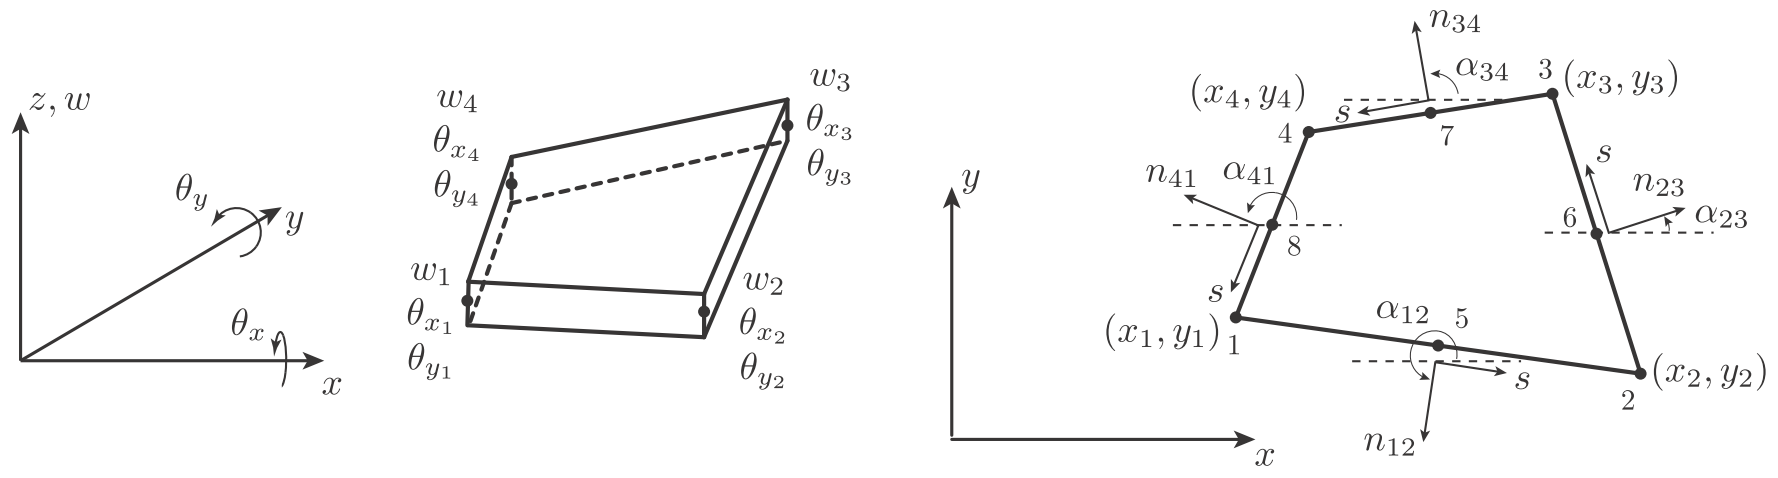
\includegraphics[width=15cm]{images/8nodeseren.png}
	\caption{DKQ DOF arrangement and geometry (source: \cite{Bar12})}
	\label{8nodeseren}
\end{figure}

\begin{equation} 
\mathbf{u^T} = 
\begin{pmatrix}
\mathbf{u_1} & \mathbf{u_2} & \mathbf{u_3} & \mathbf{u_4}
\end{pmatrix} 
\hspace{10mm}
where
\hspace{10mm}
\mathbf{u{_i}^T} = 
\begin{pmatrix}
{u_{zi}} & {\theta_{xi}} & {\theta_{yi}}
\end{pmatrix}
\label{equationBending}
\end{equation}

The nodal rotational interpolation employed is as per the 8 node serendipity quad element:

\begin{equation} 
\begin{pmatrix}
\beta_x (\xi , \eta) \\
\beta_y (\xi , \eta)
\end{pmatrix}
= \sum_{i=1}^8 \psi_i (\xi , \eta) 
\begin{pmatrix}
\beta_{xi} (\xi , \eta) \\
\beta_{yi} (\xi , \eta)
\end{pmatrix}
\label{equation20}
\end{equation}

where $\psi_i$ are the standard 8 node serendipity shape functions described by Zienkiewicz \cite{Zie77}:

\begin{gather} 
	\begin{aligned}
		&\psi_i (\xi , \eta) = \frac{-1}{4} (1 + \xi_i \xi)(1 + \eta_i \eta)(1 - \xi_i \xi - \eta_i \eta)
		\hspace{10mm}
		i = 1, 2, 3, 4 \\
		&\psi_i (\xi , \eta) = \frac{1}{2} (1 - \xi^2)(1 + \eta_i \eta)
		\hspace{10mm}
		i = 5, 7 \\
		&\psi_i (\xi , \eta) = \frac{1}{2} (1 + \xi_i \xi)(1 - \eta^2)
		\hspace{10mm}
		i = 6, 8
		\label{equation21}
	\end{aligned}
\end{gather}

and $\xi_i$ and $\eta_i$ are the natural coordinates of the 8 node serendipity element described in figure \ref{8nodeseren}.

The following derivation from equations \eqref{equation22} to \eqref{equation27} is heavily summarised from that of Barrales \cite{Bar12}. The general idea is the construction of a mapping from the standard 12 DOFs at each node to $\beta_x (\xi,\ \eta)$ and $\beta_y (\xi,\ \eta)$ across the element, the derivatives of which are curvatures as expressed in equation \eqref{equation27}.

The following quantities are required components for the mapping:

\begin{equation} 
L_{ij} = \sqrt{x_{ij}^2 + y_{ij}^2}\ ,
\hspace{10mm}
x_{ij} = x_i - x_j\ ,
\hspace{10mm}
y_{ij} = y_i - y_j
\label{equation22}
\end{equation}

\begin{gather} 
	\begin{aligned}
		&a_k = \frac{-x_{ij}}{L_{ij}^2}\ ,
		\hspace{10mm}
		b_k = \frac{3}{4} \frac{x_{ij} y_{ij}}{L_{ij}^2}\ , \\
		&c_k = \frac{\frac{1}{4} x_{ij}^2 - \frac{1}{2} y_{ij}^2}{L_{ij}^2}\ ,
		\hspace{10mm}
		d_k = \frac{-y_{ij}}{L_{ij}^2}\ ,
		\hspace{10mm}
		e_k = \frac{\frac{-1}{2} x_{ij}^2 + \frac{1}{4} y_{ij}^2}{L_{ij}^2}
		\label{equation23}
	\end{aligned}
\end{gather}

The elements of the mapping matrix are arranged as such:

\begin{equation} 
\mathbf{\Psi^x} = 
\begin{pmatrix}
\Psi_1^x \\
\vdots \\
\Psi_{12}^x
\end{pmatrix}\ ,
\hspace{10mm}
\mathbf{\Psi^y} = 
\begin{pmatrix}
\Psi_1^y \\
\vdots \\
\Psi_{12}^y
\end{pmatrix}
\label{equation24}
\end{equation}

where the vectors entries are calculated as per the following scheme:

\begin{gather} 
	\begin{aligned}
		&\Psi_{3(i-1)+1}^x (\xi , \eta) = \frac{3}{2} (a_r \psi_r (\xi , \eta) - a_s \psi_s (\xi , \eta) ) \\
		&\Psi_{3(i-1)+2}^x (\xi , \eta) = b_r \psi_r (\xi , \eta) + b_s \psi_s (\xi , \eta) \\
		&\Psi_{3(i-1)+3}^x (\xi , \eta) = \psi_i (\xi , \eta) - c_r \psi_r (\xi , \eta) - c_s \psi_s (\xi , \eta)
		\label{equation25}
	\end{aligned}
\end{gather}

\begin{gather} 
	\begin{aligned}
		&\Psi_{3(i-1)+1}^y (\xi , \eta) = \frac{3}{2} (d_r \psi_r (\xi , \eta) - d_s \psi_s (\xi , \eta) ) \\
		&\Psi_{3(i-1)+2}^y (\xi , \eta) = -\psi_i (\xi , \eta) + e_r \psi_r (\xi , \eta) + c_s \psi_s (\xi , \eta) \\
		&\Psi_{3(i-1)+3}^y (\xi , \eta) = -b_r \psi_r (\xi , \eta) - b_s \psi_s (\xi , \eta)
		\label{equation26}
	\end{aligned}
\end{gather}

with $i$ = 1, 2, 3, 4 and the relationship $(i,\ r,\ s)$ as (1, 5, 8), (2, 6, 5), (3, 7, 6) and (4, 8, 7).

Relating curvatures to displacements yield:

\begin{equation} 
\boldsymbol{\chi} = \mathbf{B}_{bend} \mathbf{U}
\label{equation27}
\end{equation}

with $\mathbf{B}_{bend}$ constructed as follows:

\begin{equation} 
\mathbf{B}_{bend} =
\begin{pmatrix}
\frac{\partial \mathbf{\Psi}^{x^T}}{\partial x} \\
\frac{\partial \mathbf{\Psi}^{y^T}}{\partial y} \\
\frac{\partial \mathbf{\Psi}^{x^T}}{\partial y} + \frac{\partial \mathbf{\Psi}^{y^T}}{\partial x}
\end{pmatrix}
\ =\ 
\begin{pmatrix}
j_{11} \frac{\partial \mathbf{\Psi}^{x^T}}{\partial \xi}  + j_{12} \frac{\partial \mathbf{\Psi}^{x^T}}{\partial \eta}  \\
j_{21} \frac{\partial \mathbf{\Psi}^{y^T}}{\partial \xi} + j_{22} \frac{\partial \mathbf{\Psi}^{y^T}}{\partial \eta} \\
j_{11} \frac{\partial \mathbf{\Psi}^{y^T}}{\partial \xi}  + j_{12} \frac{\partial \mathbf{\Psi}^{y^T}}{\partial \eta} + j_{21} \frac{\partial \mathbf{\Psi}^{x^T}}{\partial \xi} + j_{22} \frac{\partial \mathbf{\Psi}^{x^T}}{\partial \eta}
\end{pmatrix}
\label{equation28}
\end{equation}

and the inverse Jacobian entries $j_{\alpha \beta}$:

\begin{gather} 
	\begin{aligned}
		&\mathbf{J} = \frac{1}{4}
		\begin{pmatrix}
			x_{21} + x_{34} + \eta (x_{12} + x_{34}) & y_{21} + y_{34} + \eta (y_{12} + y_{34}) \\
			x_{32} + x_{41} + \xi (x_{12} + x_{34}) & y_{32} + y_{41} + \xi (y_{12} + y_{34})
		\end{pmatrix}
		\ = \ 
		\begin{pmatrix}
			J_{11} & J_{12} \\
			J_{21} & J_{22}
		\end{pmatrix} \\
		&j_{11} = \frac{J_{22}}{det[J]}\ ,
		\hspace{10mm}
		j_{12} = \frac{-J_{12}}{det[J]}\ ,
		\hspace{10mm}
		j_{21} = \frac{-J_{21}}{det[J]}\ ,
		\hspace{10mm}
		j_{22} = \frac{J_{11}}{det[J]}
		\label{equation29}
	\end{aligned}
\end{gather}

\subsection{Combined formulation}

With the separate membrane and bending B matrices developed, the combined shell B matrix $\textbf{B}_{comb.}$ can be constructed to form the element stiffness matrix.

\begin{equation} 
\textbf{K}_{el} = \textbf{B}_{comb}^T \textbf{C} \textbf{B}_{comb} 
\label{equation30}
\end{equation}

\begin{equation} 
\textbf{B}_{comb} = (\mathbf{L} + \mathbf{B}_h) + \mathbf{B}_{bend} = \mathbf{B}_{mem} + \mathbf{B}_{bend} = 
\begin{pmatrix}
\mathbf{B}_{comb1} & \mathbf{B}_{comb2} & \mathbf{B}_{comb3} & \mathbf{B}_{comb4}
\end{pmatrix}
\label{equation31}
\end{equation}

The combination of $\textcolor{blue}{membrane}$ and $\textcolor{red}{bending}$ matrices must consider the DOF ordering of each component and the relation to the total shell DOF ordering, as shown below:

\begin{equation} 
\mathbf{u}_i = 
\begin{pmatrix}
\textcolor{blue}{u_{xi}} \\ 
\textcolor{blue}{u_{yi}} \\ 
\textcolor{red}{u_{zi}} \\ 
\textcolor{red}{\theta_{xi}} \\ 
\textcolor{red}{\theta_{yi}} \\ 
\textcolor{blue}{\theta_{zi}} \\ 
\end{pmatrix}
\label{equation32}
\end{equation}

Considering this, the addition of the membrane (basic and higher order) B matrices and the bending B matrix is conducted as follows:

\begin{multline}
	\mathbf{B}_{comb\ i} = \left(
	\begin{matrix}
		\textcolor{blue}{\mathbf{B}_{mem}[1,3(i-1) + 1]} & \textcolor{blue}{\mathbf{B}_{mem}[1,3(i-1) + 2]} & 0 \\ 
		\textcolor{blue}{\mathbf{B}_{mem}[2,3(i-1) + 1]} & \textcolor{blue}{\mathbf{B}_{mem}[2,3(i-1) + 2]} & 0 \\ 
		0 & 0 & \textcolor{red}{\mathbf{B}_{bend}[1,3(i-1) + 1]} \\ 
		0 & 0 & \textcolor{red}{\mathbf{B}_{bend}[2,3(i-1) + 1]} \\
		0 & 0 & \textcolor{red}{\mathbf{B}_{bend}[3,3(i-1) + 1]} \\
		\textcolor{blue}{\mathbf{B}_{mem}[3,3(i-1) + 1]} & \textcolor{blue}{\mathbf{B}_{mem}[3,3(i-1) + 2]} & 0 \\
	\end{matrix}\right.                
	\\
	\left.
	\begin{matrix}
		0 & 0 & \textcolor{blue}{\mathbf{B}_{mem}[1,3(i-1) + 3]} \\ 
		0 & 0 & \textcolor{blue}{\mathbf{B}_{mem}[2,3(i-1) + 3]} \\ 
		\textcolor{red}{\mathbf{B}_{bend}[1,3(i-1) + 2]} & \textcolor{red}{\mathbf{B}_{bend}[1,3(i-1) + 3]} & 0 \\ 
		\textcolor{red}{\mathbf{B}_{bend}[2,3(i-1) + 2]} & \textcolor{red}{\mathbf{B}_{bend}[2,3(i-1) + 3]} & 0 \\
		\textcolor{red}{\mathbf{B}_{bend}[3,3(i-1) + 2]} & \textcolor{red}{\mathbf{B}_{bend}[3,3(i-1) + 3]} & 0 \\
		0 & 0 & \textcolor{blue}{\mathbf{B}_{mem}[3,3(i-1) + 3]} \\
	\end{matrix}\right)
	\label{equation33}
\end{multline}

\section{Stiffness matrix implementation}

With the formulation of the ANDES-DKQ shell element established, a high level overview of it's implementation in KRATOS is discussed in this section.

The new quad element is implemented in the files $\texttt{shell\_thin\_element\_3D4N.hpp}$ and\break$\texttt{shell\_thin\_element\_3D4N.cpp}$, which are compiled into the 'StructuralMechanicsApplication' module of Kratos. Similar to the DSG triangle element, the new ANDES-DKQ element class $\texttt{ShellThinElement3D4N}$ is inherited from the Kratos base class $\texttt{Element}$ and also leverages the existing capabilities other Kratos classes offer. The general workflow of calculating the ANDES-DKQ stiffness matrix is as follows:

\begin{figure}[H]
	% Define block styles
	\tikzstyle{virtual} = [rectangle, minimum width=3cm, minimum height=1cm, text centered, draw=black, fill=orange!30]
	\tikzstyle{process} = [rectangle, minimum width=3cm, minimum height=1cm, text centered, draw=black, fill=white!30]
	\tikzstyle{arrow} = [thick,->,>=stealth]
	\begin{tikzpicture}[node distance = 1.9cm, auto]
% Place nodes
\node [process] (CalculateLocalSystem) {$\texttt{CalculateLocalSystem()}$};
\node [process, right of=CalculateLocalSystem, xshift = 4cm] (CalculateAll) {$\texttt{CalculateAll()}$};
\node [process, below of=CalculateAll, xshift = -0cm] (InitializeCalculationData) {$\texttt{InitializeCalculationData()}$};
\node [process, below of=InitializeCalculationData, yshift = -0cm] (CalculateSectionResponse) {$\texttt{CalculateSectionResponse()}$};
\node [process, below of=CalculateSectionResponse, yshift = -0cm] (FinalizeCalculations) {$\texttt{FinalizeCalculations()}$};
% Draw edges
\draw [arrow] (CalculateLocalSystem) -- (CalculateAll);
\draw [arrow] (CalculateAll) -- (InitializeCalculationData);
\draw [arrow] (InitializeCalculationData) -- (CalculateSectionResponse);
\draw [arrow] (CalculateSectionResponse) -- (FinalizeCalculations);
\end{tikzpicture}
	\caption{High level overview of ANDES-DKQ element workflow}
	\label{andesworkflow}
\end{figure}

As per the DSG triangle element, the re-implemented virtual method $\texttt{CalculateLocalSystem()}$ is called by the KRATOS framework automatically for every $\texttt{ShellThinElement3D4N}$ in the job definition. This method simply calls $\texttt{CalculateAll()}$, which initializes calculating the stiffness matrix by calling $\texttt{InitializeCalculationData(),\ CalculateGaussPointContribution()}$ and $\texttt{FinalizeCalculations()}$.

$\texttt{InitializeCalculationData()}$ is called first, and pre-calculates quantities so they can be removed from the Gauss loop. These quantities include the ANDES basic lumping matrix $\textbf{L}$, the ANDES higher order strain-displacement matrices $\textbf{B}_{hi}$ and all DKQ coefficients in equation  \eqref{equation23}.

$\texttt{CalculateAll()}$ then calls $\texttt{CalculateGaussPointContribution()}$ which starts the Gauss integration loop. At each Gauss point $\texttt{CalculateGaussPointContribution()}$ performs Gauss integration of the expression $\textbf{K}_{contribution}$ = $\textbf{B}_{comb}^T \textbf{C} \textbf{B}_{comb}\  dA$, with the current $\textbf{B}_{comb}$ determined by calling $\texttt{CalculateBMatrix()}$.

With the Gauss integration complete, $\texttt{CalculateAll()}$ lastly calls $\texttt{FinalizeCalculations()}$ which transforms the calculated element stiffness from local to global coordinates.

The following pseudocode summarises the key calls and operations involved in calculating the ANDES-DKQ element stiffness matrix.

\begin{algorithm}
	\onehalfspacing
	\caption{ANDES-DKQ element stiffness matrix pseudocode}\label{ANDES-DKQ element stiffness matrix}
	\begin{algorithmic}[1]
		\Require Coordinate transformation instance
		\State \textbf{call} $\texttt{CalculateAll()}$
		\State Resize $LHS$ and $RHS$
		\State \textbf{call} $\texttt{InitializeCalculationData}(data)$
		\State \hspace{\algorithmicindent}Calculate integration areas $dA = w_i \cdot detJ(xi,\ eta)$
		\State \hspace{\algorithmicindent}Determine basic membrane strain displacement $L$
		\State \hspace{\algorithmicindent}Construct membrane higher order filter matrix $H$
		\State \hspace{\algorithmicindent}Arrange higher order natural strain matrices $Q_i$
		\State \hspace{\algorithmicindent}Transform $Q_i$ into $B_{hi}$
		\State \hspace{\algorithmicindent}Determine $\bar{B_h}$
		\State \hspace{\algorithmicindent}Pre-calculate all DKQ coefficients
		\While{$gaussPoint$ < 4}
		\State \textbf{call} $\texttt{CalculateGaussPointContribution}(data)$
		\State \hspace{\algorithmicindent}\textbf{call} $\texttt{CalculateBMatrix}(data)$
		\State \hspace{\algorithmicindent}\hspace{\algorithmicindent} Calculate and combine $B_{mem}$ and $B_{bend}$ into $B$
		\State \hspace{\algorithmicindent}\textbf{call} $\texttt{CalculateSectionResponse}(data)$
		\State \hspace{\algorithmicindent}\hspace{\algorithmicindent} Calculate material properties $C$
		\State \hspace{\algorithmicindent}Add stiffness matrix Gauss point contribution to $LHS$
		\EndWhile
		\State Modify $RHS$ residual vector
		\State \textbf{call} $\texttt{FinalizeCalculations}(data,\ displacements,\ LHS,\ RHS)$
		\State \textbf{call} $\texttt{AddBodyForces}(data,\ RHS)$
	\end{algorithmic}
\end{algorithm}

\section{Mass matrix formulation}

The mass matrix is necessary to facilitate dynamic analysis with the thin quadrilateral shell element. As per the existing KRATOS shell elements, a lumped mass approach is employed which results in a diagonal mass matrix.
\begin{equation} 
\mathbf{M} =  
\begin{pmatrix}
\mathbf{M}_1 & \mathbf{0} & \mathbf{0} & \mathbf{0}\\
\mathbf{0} & \mathbf{M}_2 & \mathbf{0} & \mathbf{0}\\
\mathbf{0} & \mathbf{0} & \mathbf{M}_3 & \mathbf{0}\\
\mathbf{0} &\mathbf{0} & \mathbf{0} & \mathbf{M}_4
\end{pmatrix}
\hspace{10mm}
where
\hspace{10mm}
\mathbf{M}_i =  
\begin{pmatrix}
\bar{m} & 0 & 0 & 0 & 0 & 0\\
0 & \bar{m} & 0 & 0 & 0 & 0\\
0 & 0 & \bar{m} &0 & 0 & 0\\
0 & 0 & 0 & 0 & 0 & 0\\
0 & 0 & 0 & 0 & 0 & 0\\
0 & 0 & 0 & 0 & 0 & 0
\end{pmatrix}
\label{eqt15}
\end{equation}

The general lumped mass is determined for a multi-ply material with $n$ plies each of $t_i$ thickness and $\rho_i$ density as follows:

\begin{equation} 
\bar{m} = \frac{A}{4} \sum_{i=1}^n \rho_i t_i
\label{eqt16}
\end{equation}

For a single layer material of area $A$ this reduces to:

\begin{equation} 
\bar{m} = \frac{A}{4} \rho t
\label{eqt17}
\end{equation}

\section{Stress and strain recovery}

The stresses and strains of the ANDES-DKT quadrilateral element are recovered in a similar way to the DSG triangle, with the added complication of the multiple Gauss points.

The non-zero local strains ($\epsilon_{zz},\ \epsilon_{xz},\ \epsilon_{yz} = 0$) of the 4 noded 3 parameter element can be arranged in a vector form:

\begin{equation} 
\boldsymbol{\epsilon}^T = \begin{pmatrix}
\boldsymbol{\epsilon}_1 & \boldsymbol{\epsilon}_2 & \boldsymbol{\epsilon}_3 & \boldsymbol{\epsilon}_4
\end{pmatrix}
\hspace{5mm}
with
\hspace{5mm}
\boldsymbol{\epsilon}^T_i = \begin{pmatrix}
\epsilon_{xx} & \epsilon_{xx} & 2\epsilon_{xy} & \epsilon_{xx} & \kappa_{xx} & \kappa_{yy} & 2\kappa_{xy} 
\end{pmatrix}
\label{eqqrec1}
\end{equation}

The nodal strain vector is recovered from the displacement field by applying the strain displacement matrix, which varies over the element.

\begin{equation} 
\boldsymbol{\epsilon}(\xi,\ \eta) = \mathbf{B}(\xi,\ \eta) \mathbf{u}(\xi,\ \eta)
\label{eqqrec2}
\end{equation}

As per the DSG triangle, the strains and stresses are calculated at the Gauss points of the element, with the ANDES-DKT element having four Gauss points ($j = 1,\ 2,\ 3,\ 4$). Thus, the strain vector at each Gauss point $j$ is recovered from the discrete nodal displacements $\hat{\mathbf{u}}_i$ as follows:

\begin{equation} 
\boldsymbol{\epsilon}_{GP_j} = \mathbf{B}(\xi_j,\ \eta_j) \sum_{i=1}^{4\ nodes} N_i(\xi_j,\ \eta_j) \hat{\mathbf{u}}_i
\label{eqqrec3}
\end{equation}

With the strains determined, the stresses at each Gauss point are recovered with the material matrix (which in the general case may vary over the element).

\begin{equation} 
\boldsymbol{\sigma}_{GP_j} = \mathbf{C}_{GP_j}\ \boldsymbol{\epsilon}_{GP_j}
\label{eqqrec4}
\end{equation}

The general implementation of the stress and strain recovery described above is illustrated in the following pseudocode.

\begin{algorithm}
	\onehalfspacing
	\caption{ANDES-DKT quadrilateral element stress and strain recovery}
	\label{ANDES-DKT quadrilateral element stress and strain recovery}
	\begin{algorithmic}[1]
		\Require $requestedQuantity$, calculation of nodal displacements
		\State \textbf{call} $\texttt{InitializeCalculationData}(data)$
		\State \hspace{\algorithmicindent}Calculate constant components of strain-displacement matrix $B$
		\State \hspace{\algorithmicindent}Retrieve element $localDisplacements$
		
		\While{$gaussPoint$ < 4}
		\State \textbf{call} $\texttt{CalculateGaussPointContribution}(data)$
		\State \hspace{\algorithmicindent}\textbf{call} $\texttt{CalculateBMatrix}(data)$
		\State \hspace{\algorithmicindent}\hspace{\algorithmicindent} Calculate combined $B$ at current $gaussPoint$
		\State $generalizedStrains$ = product$(B,\ localDisplacements)$
		\If{$requestedQuantity$ requires stress} 
		\State \textbf{call} $\texttt{CalculateSectionResponse}(data)$
		\State $generalizedStresses$ = product $(C,\ generalizedStrains)$
		\State Decimal correction of $generalizedStresses$
		\EndIf
		\State Decimal correction of $generalizedStrains$ 
		\If{$requestedQuantity$ requires local orientation} 
		\State Rotate $requestedQuantity$ to local orientation
		\EndIf
		\State Assemble $requestedQuantity$ into $outputMatrix$
		\If{$requestedQuantity$ requires global orientation} 
		\State Rotate $outputMatrix$ to global orientation
		\EndIf
		\State Interpolate $outputMatrix$ to standard Gauss points for visualisation
		\EndWhile
	\end{algorithmic}
\end{algorithm} %thin quad
%%%%%%%%%%%%%%%%%%%%%%%%%%%%%%%%%%%%%%%%%%%%%%%%%%%%%%%%
%%%%                                              %%%%%%
%%%%  Author: Peter Wilson                        %%%%%%
%%%%                                              %%%%%%
%%%%  Validation of elements                          %%%%%%
%%%%                                              %%%%%%
%%%%%%%%%%%%%%%%%%%%%%%%%%%%%%%%%%%%%%%%%%%%%%%%%%%%%%%%


%fref generates automatically the respective abreviation/word in the text for the reference. You just have to define a label starting with the respective keyword.
%english: chap, sec, fig, eq, app
%deutsch: chap/kap, abs, abb, gl, anh
%see http://ctan.space-pro.be/tex-archive/macros/latex/contrib/fancyref/fancyref.pdf for more information



\chapter{Validation of the elements}

\renewcommand{\Thema}{Validation of the elements}

\lettrine[lines=2]{V}{alidation} is as important to proper engineering analysis as the calculations performed. The following tests across linear statics, geometrically non-linear statics, linear and non-linear dynamics, quantity recovery and composites interrogate the correct implementation of the element formulations and also gives an initial indication of their performance. 

Unless noted otherwise, materials are isotropic linear elastic.

\section{Linear static tests: shell obstacle course}
\label{section:shell obstacle course}

Considered as the standard benchmark for shell elements, the shell obstacle course proposed by Belytschko \cite{Bel85} runs the elements through 3 problems involving complex loading states. These complex loading states often pose difficulties for un-enhanced elements, which are also tested here.

The \textit{Basic-DKQ} element is a linear quadrilateral element with an un-enhanced membrane formulation and the DKQ bending formulation. Refer to Appendix \ref{sec:Basic-DKQ quadrilateral formulation} for full details. Any performance differences that arise between this element and the ANDES-DKQ element can be attributed to the ANDES element technology.

The \textit{Basic-T3} element is a linear triangular element with an un-enhanced shear formulation and no correction to the shear component of the material matrix. Refer to Appendix \ref{sec:Basic-T3 quadrilateral formulation} for full details. Any performance differences that arise between this element and the DSG element can be attributed to the DSG element technology.

Furthermore, context of element performance is provided by including results from the existing \textit{KRATOS Q4} five parameter linear quadrilateral element (EAS-MITC formulation) and the \textit{KRATOS T3} three parameter linear triangle element (ANDES-DKT formulation).
\newpage
\subsection{Scordelis-Lo roof}
%
%\begin{wrapfigure}{r}{0.45\textwidth}
%	\centering
%	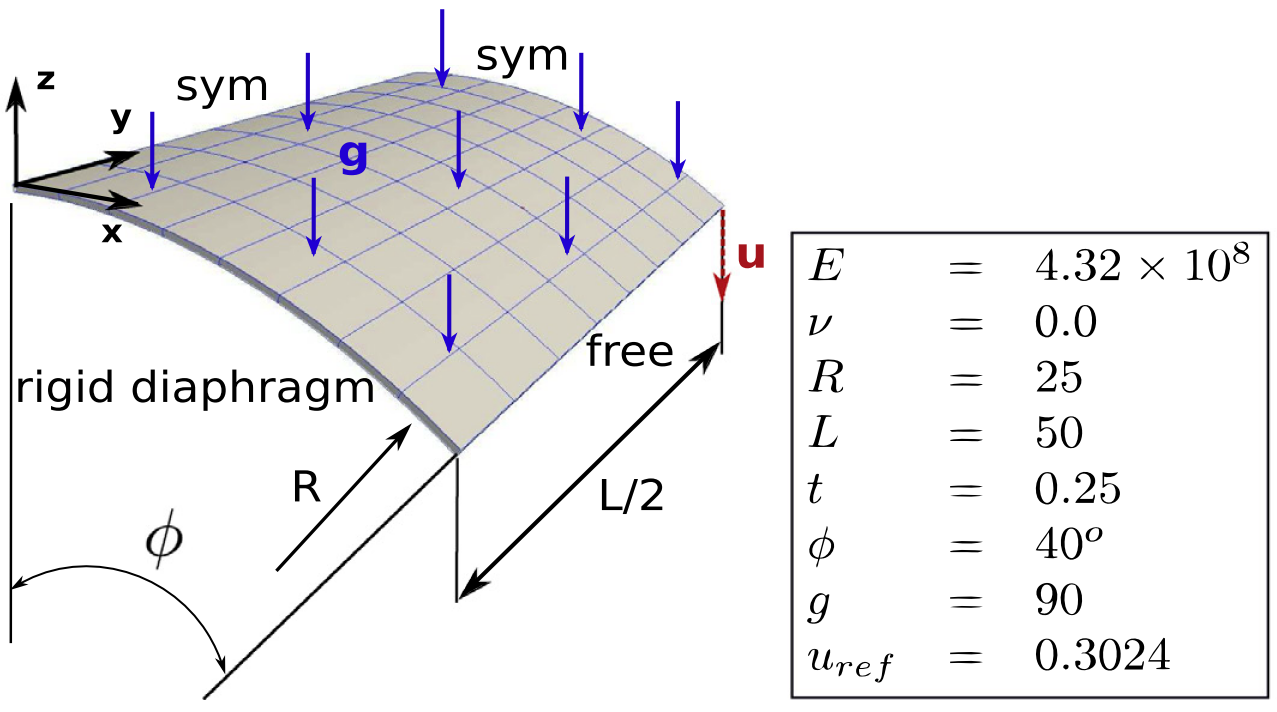
\includegraphics[width=0.40\textwidth]{images/scordelisroof.png}
%	\caption{Definition of the Scordelis-Lo roof benchmark\cite{Bou13}}
%\end{wrapfigure}

The first problem of the shell obstacle course is the Scordelis-Lo roof, which is part of a cylindrical shell fixed by rigid diaphragms at its axial ends. The loading is a pseudo-gravity distributed load that has a magnitude of 90. Due to symmetry, only a quarter of the shell is modelled with a structured mesh. The key result is the vertical displacement of the lateral side at the midpoint, denoted by $\textcolor{red}{u}$ in the following diagram. The reference value is $u_{ref} = 0.3024$.
 
  \begin{figure}[H]
 	\centering
 	\def\svgwidth{\columnwidth}
 	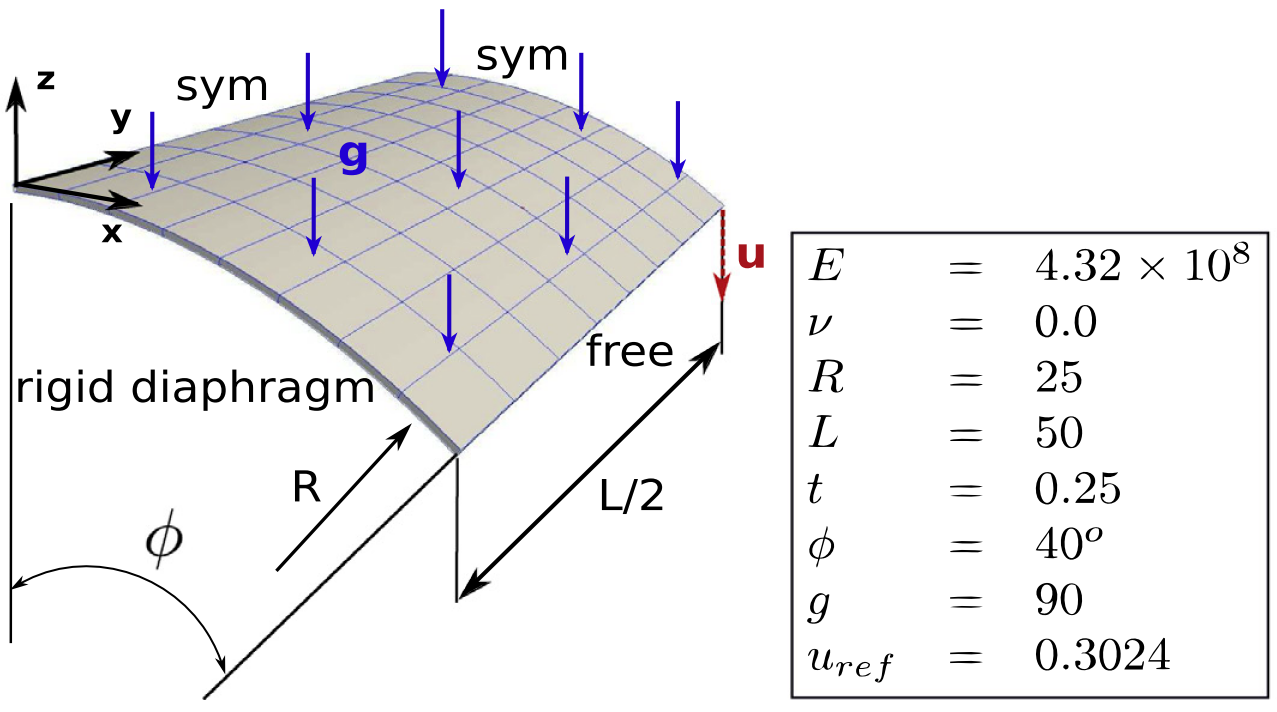
\includegraphics[width=7.3cm]{images/scordelisroof.png}
 	\caption{Definition of the Scordelis-Lo roof benchmark\cite{Bou13}}
 \end{figure}
 
\begin{figure}[H]
	\subfloat[Quadrilateral element convergence for the Scordelis-Lo roof benchmark]
	{\label{ref_label2}
		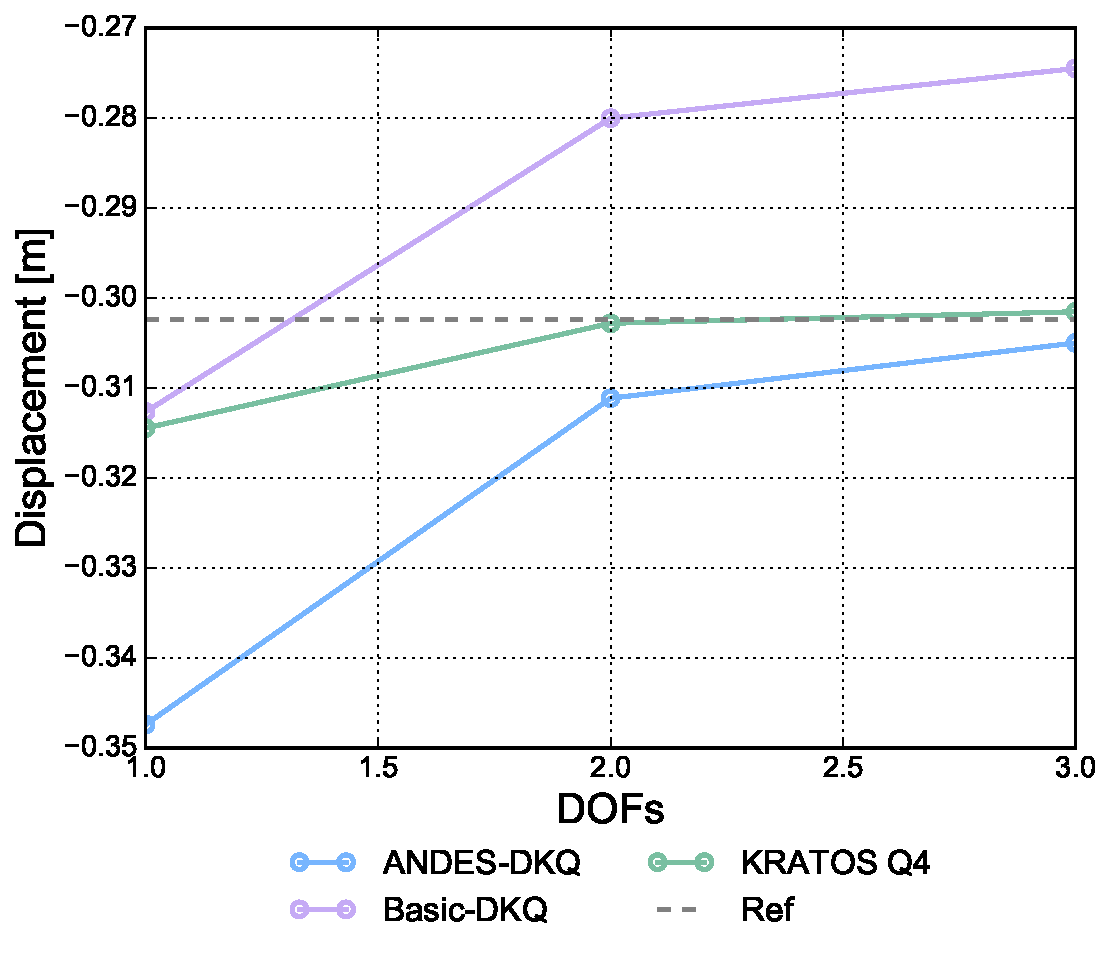
\includegraphics[width=7.3cm]
		{scordelis_structured_quad_results.pdf}}
	\subfloat[Triangle element convergence for the Scordelis-Lo roof benchmark]
	{\label{ref_label2}
		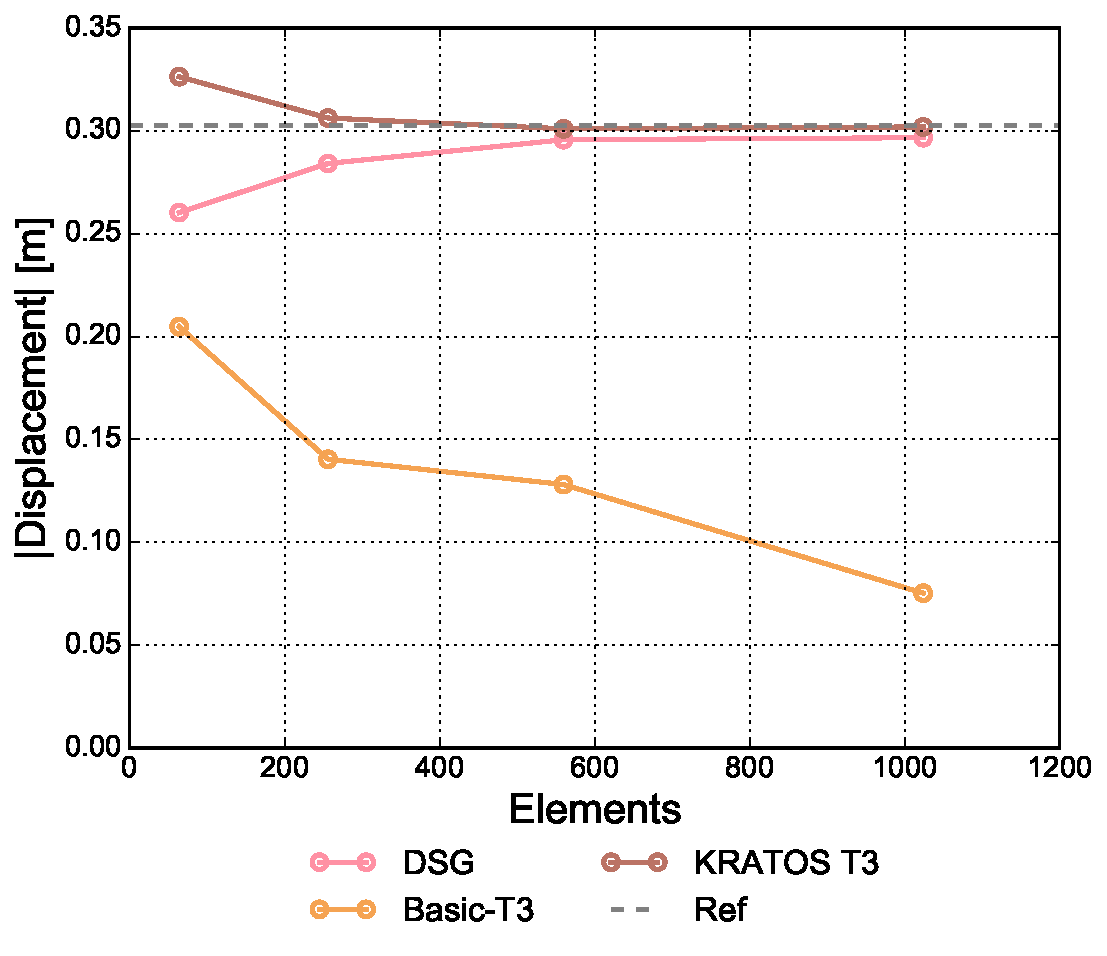
\includegraphics[width=7.3cm]
		{scordelis_structured_tri_results.pdf}}
	\caption{\label{ref_label_overall}Scordelis-Lo roof benchmark results}
\end{figure}

The convergence graphs above indicate the ANDES-DKQ and DSG elements agree with the reference solution. Conversely, the Basic-T3 element shows very poor performance. Given that the Basic-DKQ performs well (which is immune to transverse shear locking), it is suspected that transverse shear locking is crippling the Basic-T3 element, while the DSG element technology effectively mitigates this for the DSG element. 
\newpage
\subsection{Pinched cylinder}
%
%\begin{wrapfigure}{r}{0.45\textwidth}
%	\centering
%	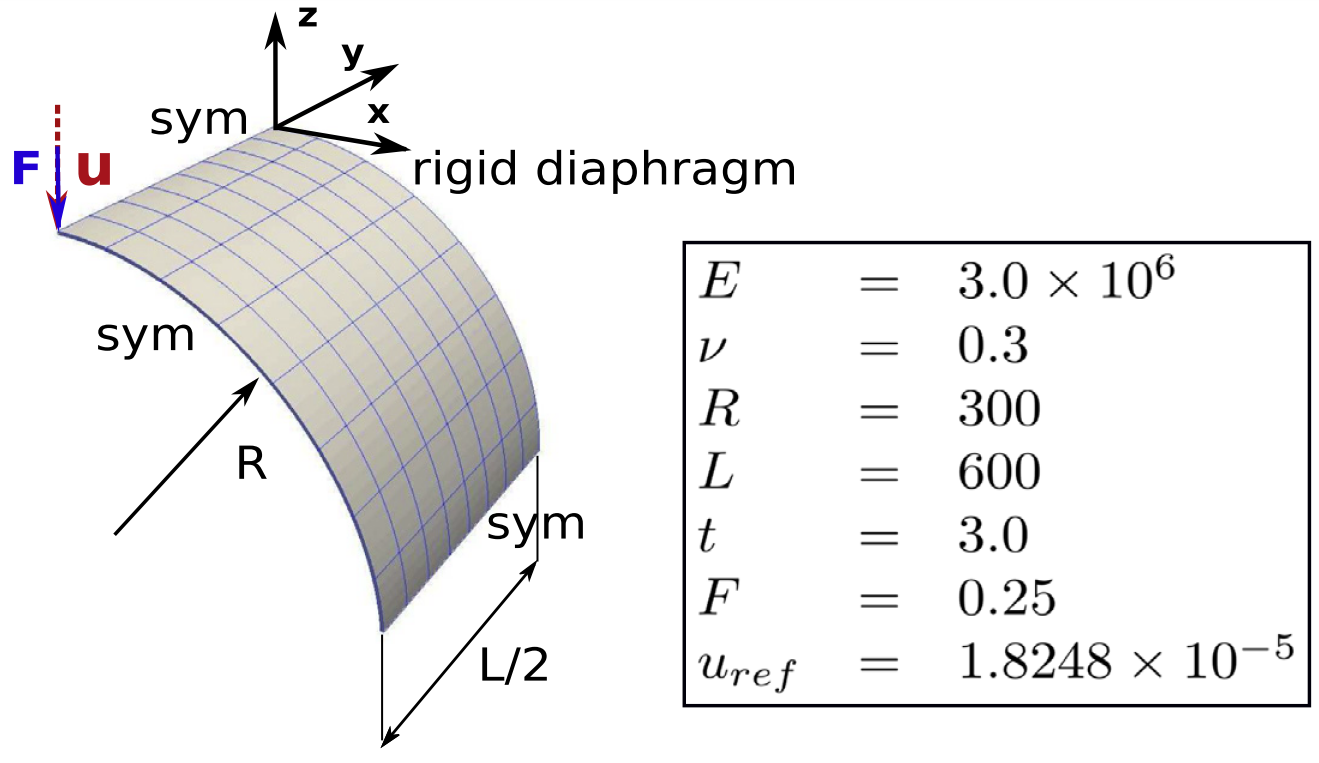
\includegraphics[width=0.4\textwidth]{images/pinchedcylinder.png}
%	\caption{Definition of the pinched cylinder benchmark\cite{Bou13}}
%\end{wrapfigure}

The second problem of the shell obstacle course is the pinched cylinder, which considers a cylindrical shell fixed by rigid diaphragms at its axial ends. The loading consists of two opposing compressive point loads at the centre of the shell. Due to symmetry only an eighth of the shell is modelled with a structured mesh. The key result is the vertical displacement under the point load, denoted by $\textcolor{red}{u}$ in the following diagram. The reference value is $u_{ref} =  1.8248\ \times\ 10^{-5}$. 
 
 \begin{figure}[H]
 	\centering
 	\def\svgwidth{\columnwidth}
 	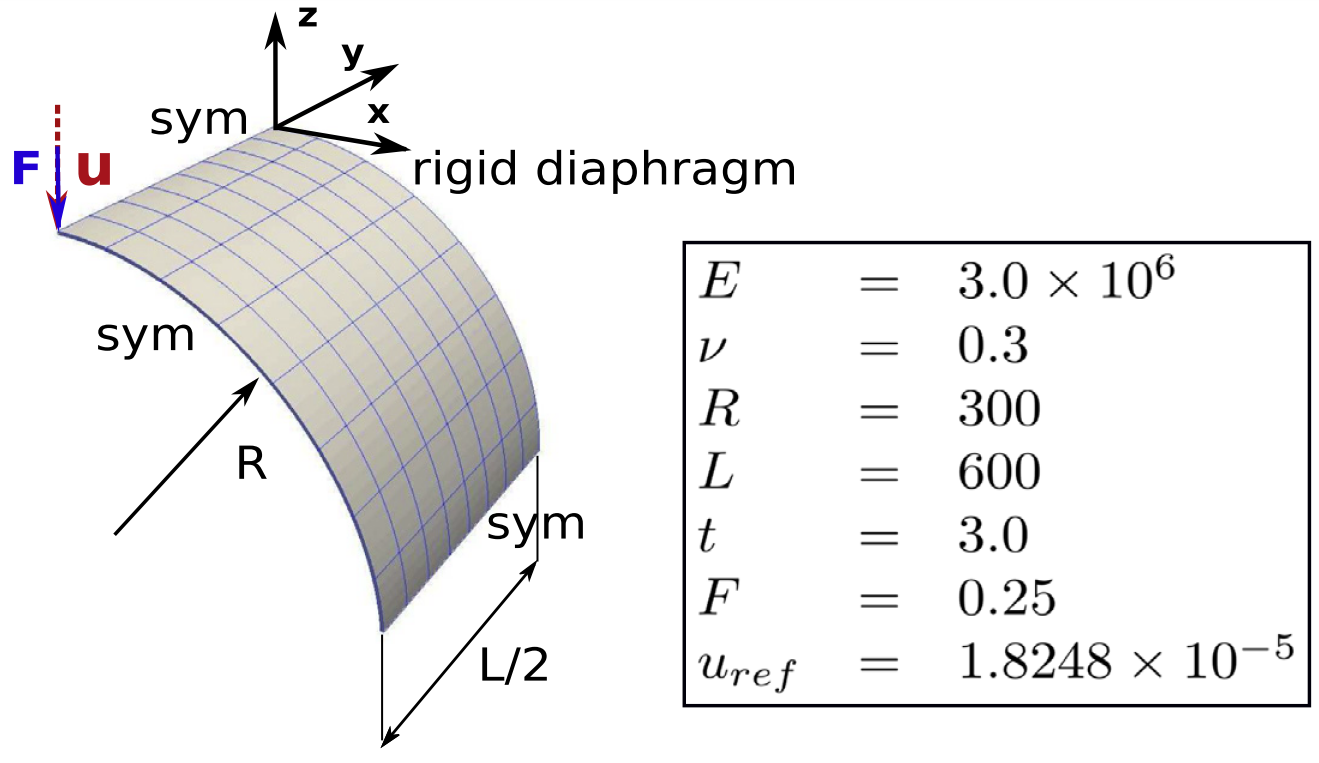
\includegraphics[width=7.3cm]{images/pinchedcylinder.png}
 	\caption{Definition of the pinched cylinder benchmark\cite{Bou13}}
 \end{figure}
 
\begin{figure}[H]
	\subfloat[Quadrilateral element convergence for the pinched cylinder benchmark]
	{\label{ref_label2}
		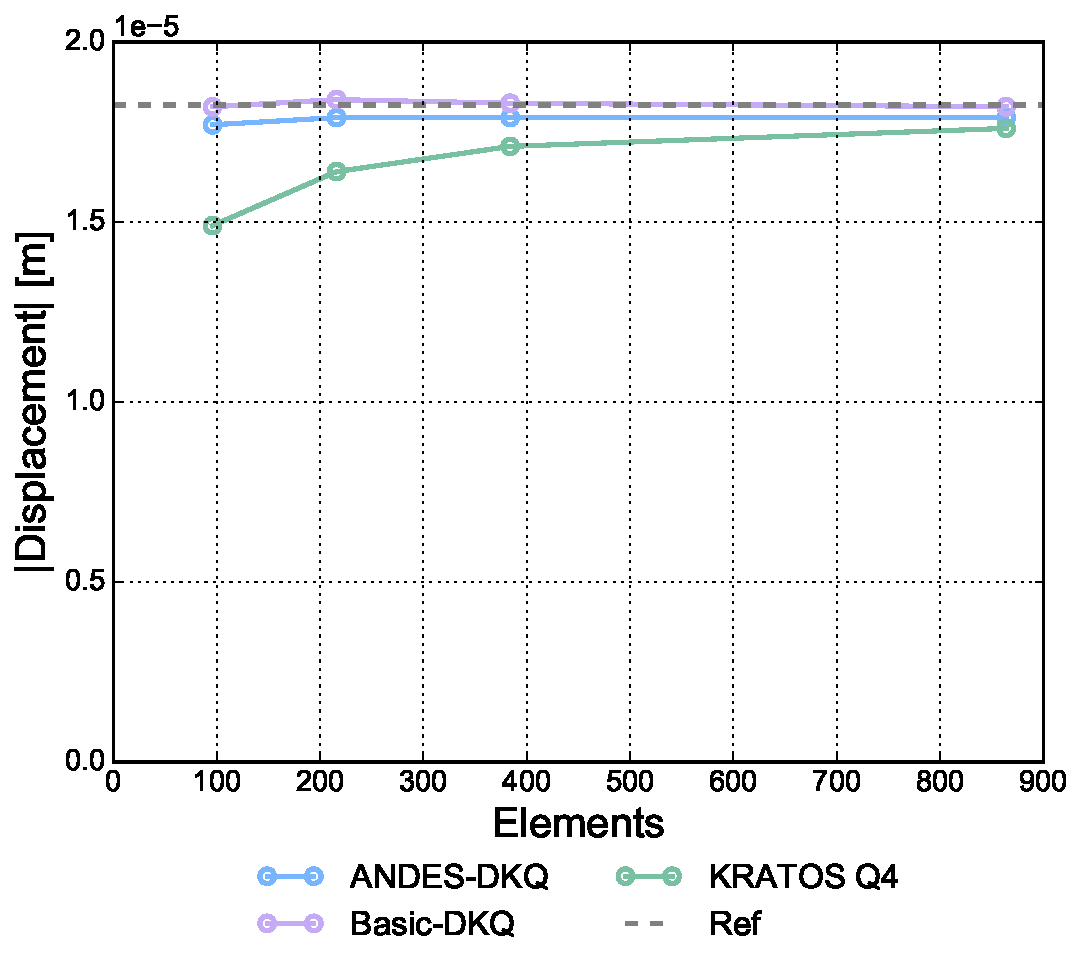
\includegraphics[width=7.3cm]
		{pinched_cyl_structured_quad_results.pdf}}
	\subfloat[Triangle element convergence for the pinched cylinder benchmark]
	{\label{ref_label2}
		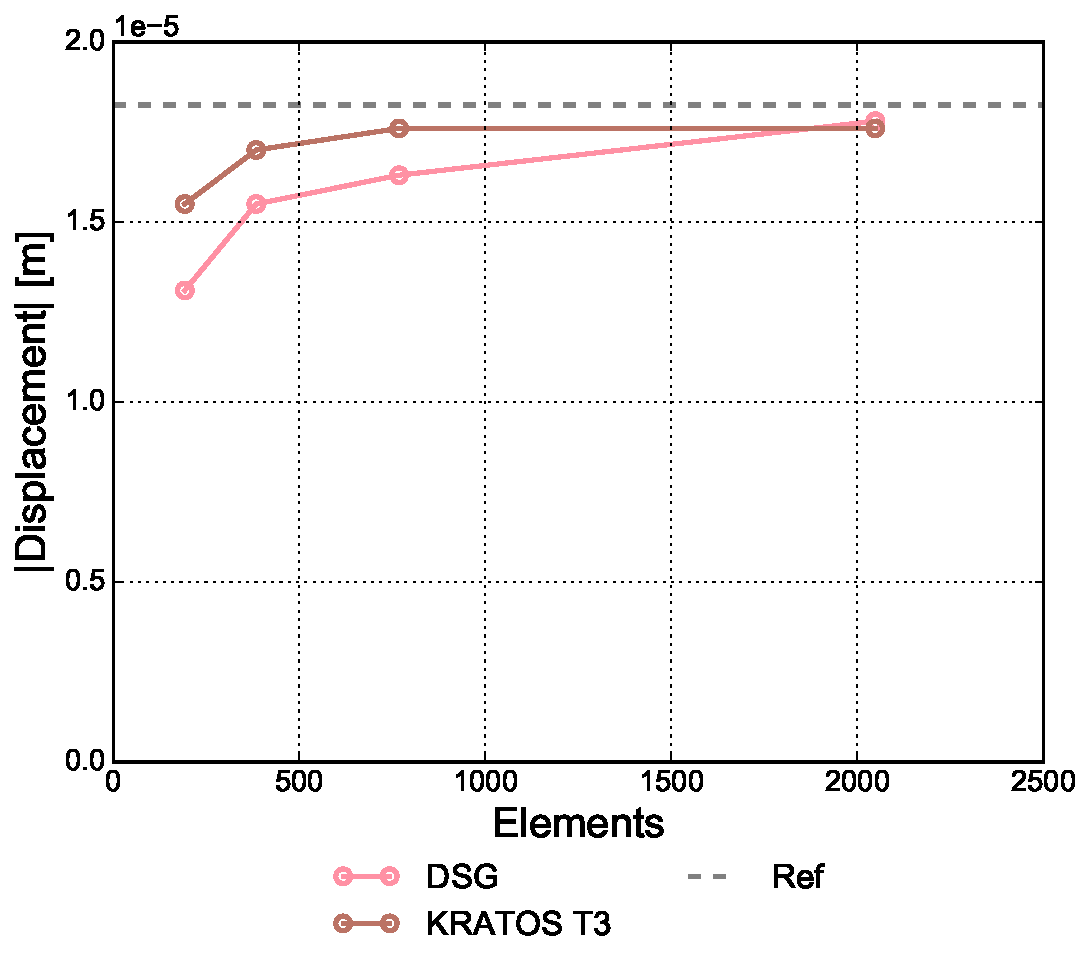
\includegraphics[width=7.3cm]
		{pinched_cyl_structured_tri_results.pdf}}
	\caption{\label{ref_label_overall}Pinched cylinder benchmark results}
\end{figure}

 The good performance of both the ANDES-DKQ and DSG elements is demonstrated in the convergence graphs above. The Basic-T3 results were in the order of $1\times10^{-3}$ (roughly 100 times greater than the reference solution) and were omitted from the graph for clarity of scale. Once again, it is clear that the computationally inexpensive DSG element technology drastically improves performance from the un-enhanced Basic-T3 to the DSG element.
\newpage
\subsection{Pinched hemisphere}
%
%\begin{wrapfigure}{r}{0.45\textwidth}
%	\centering
%	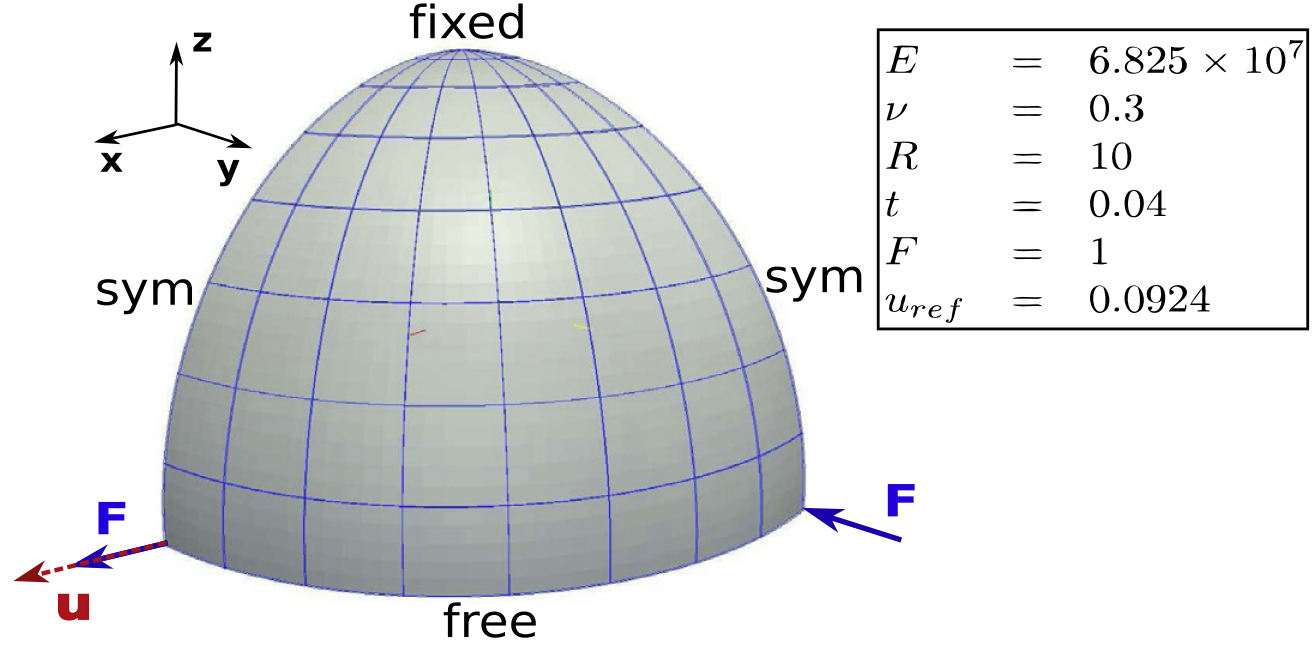
\includegraphics[width=0.4\textwidth]{images/pinchedhemisphere.png}
%	\caption{Definition of the pinched hemisphere benchmark \cite{Bou13}}
%\end{wrapfigure}

The last test in the shell obstacle course is the pinched hemisphere, which considers a hemispherical shell loaded with opposing point loads along its equator. Due to symmetry only a quarter of the shell is modelled with an unstructured mesh. The key result is the 'x' displacement along one of the point loads, denoted by $\textcolor{red}{u}$ in the following diagram. The reference value is $u_{ref} =  0.0924$. 

\begin{figure}[H]
	\centering
	\def\svgwidth{\columnwidth}
	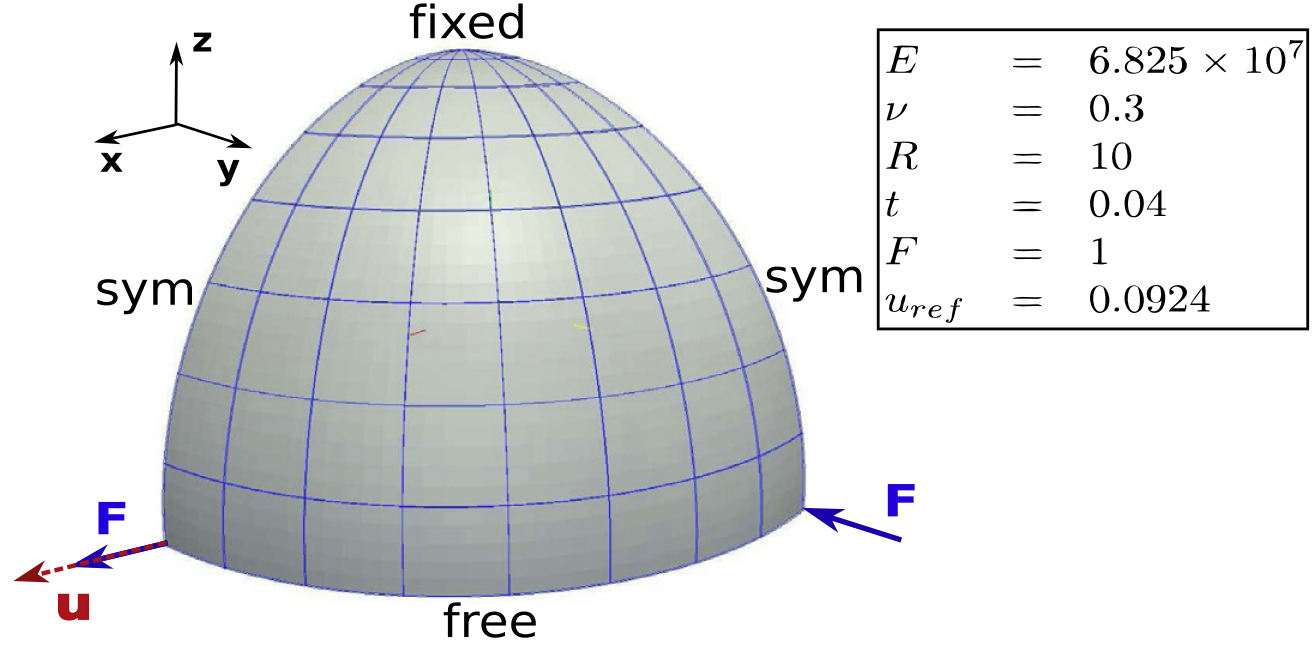
\includegraphics[width=7.3cm]{images/pinchedhemisphere.png}
	\caption{Definition of the pinched hemisphere benchmark \cite{Bou13}}
\end{figure}

\begin{figure}[H]
	\subfloat[Quadrilateral element convergence for the pinched hemisphere benchmark]
	{\label{ref_label2}
		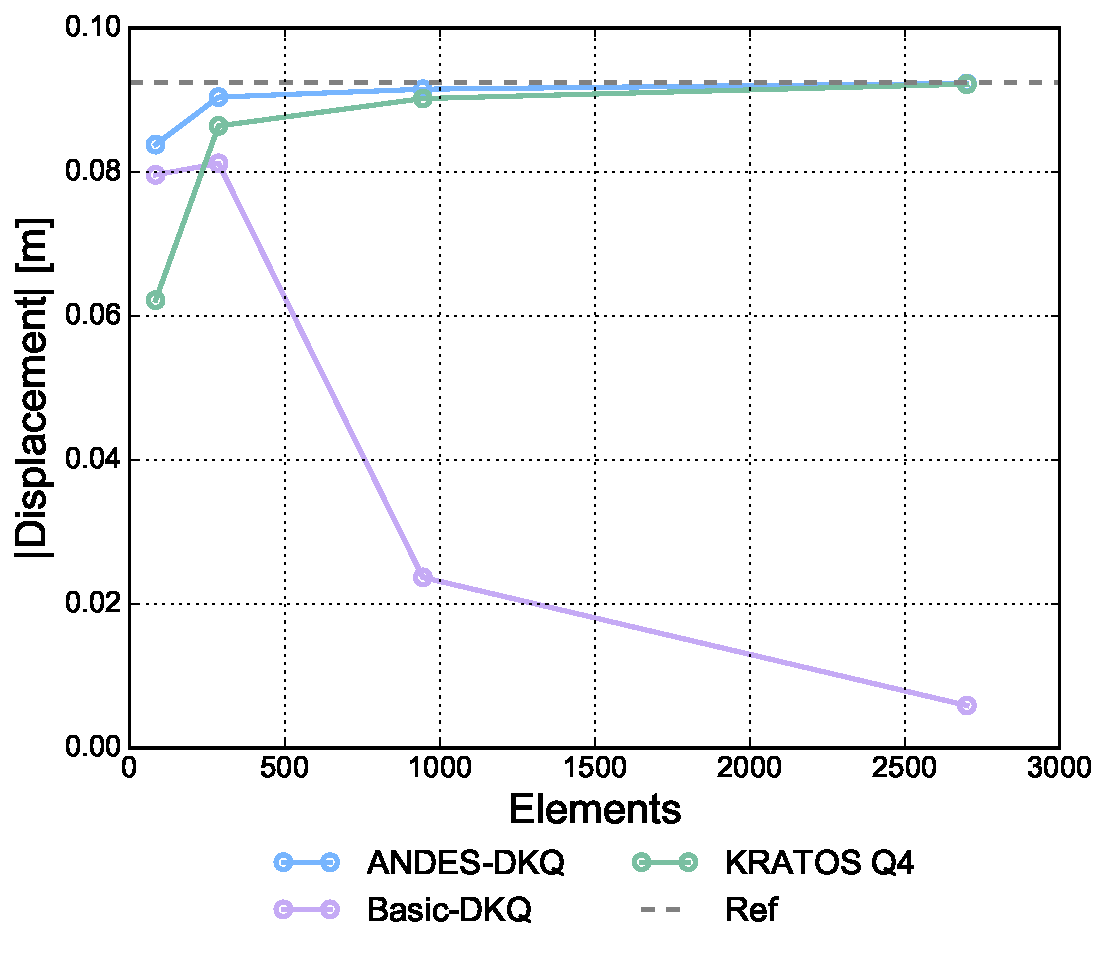
\includegraphics[width=7.3cm]
		{pinched_hemi_quad_results.pdf}}
	\subfloat[Triangle element convergence for the pinched hemisphere benchmark]
	{\label{ref_label2}
		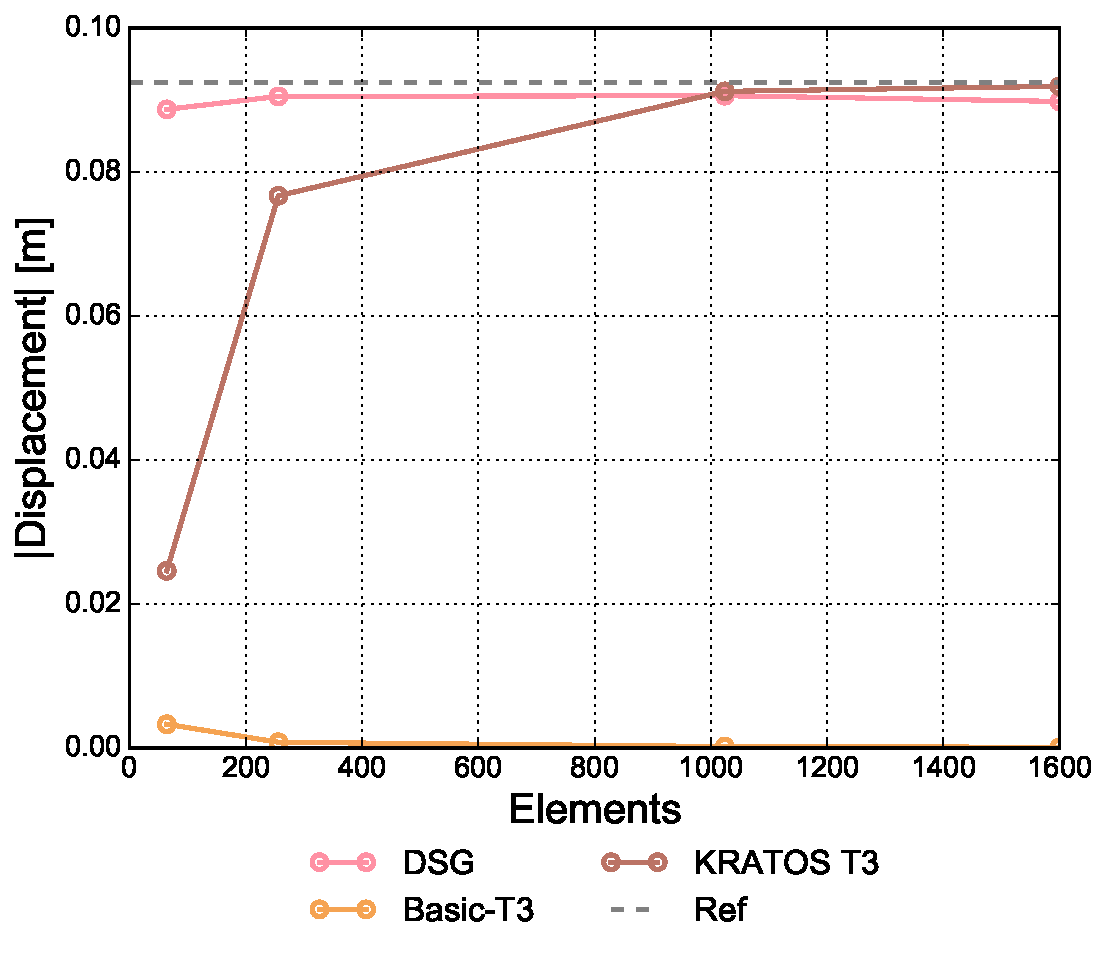
\includegraphics[width=7.3cm]
		{pinched_hemi_tri_results.pdf}}
	\caption{\label{ref_label_overall}Pinched hemisphere benchmark results}
\end{figure}

The ANDES-DKQ and DSG elements both perform well in the final statics test, as per the convergence graphs above. It is observed that the Basic-DKQ element appears to exhibit membrane locking corresponding to the high double curvature of the problem ($R_1=R_2 = 10$) compared to the Scordelis-Lo roof ($R_1= 10,\ R_2 = \infty$) and the pinched cylinder ($R_1= 300,\ R_2 = \infty$). The ANDES element technology clearly prevents this deleterious effect. The poor performance of the Basic-T3 element compared to the DSG element once again highlights the effectiveness of the DSG element technology in preventing transverse shear locking.
\newpage
\section{Geometrically non-linear static tests}

Large rotations and displacements mark the departure from geometrically linear to non-linear analyses. By employing the already implemented EICR CE formulation as described in section \ref{EICR overview}, both shell elements can be extended from linear geometry limitations to handle large displacements, provided deformational strains remain small. The performance of the elements in geometrically non-linear problems are considered with two benchmarks.

\subsection{Hinged cylindrical roof}
\label{validation:hinged cyl roof}
The first geometrically non-linear benchmark is the snap-through of a hinged cylindrical roof under a central point load $P_{max} = 3000$ \cite{Sze2004}. As per the diagram below, the roof geometry is defined with the parameters: $L = 254,\ R = 2540,\ \theta=0.1\ rad$ and $h = 12.7$. The material is defined with a Young's modulus $E = 3102.75$ and Poisson's ratio of $\nu = 0.3$.

 
\begin{figure}[H]
	%\centering
	\subfloat[Hinged cylindrical roof definition \cite{Sze2004}]
	{\label{ref_label1}
		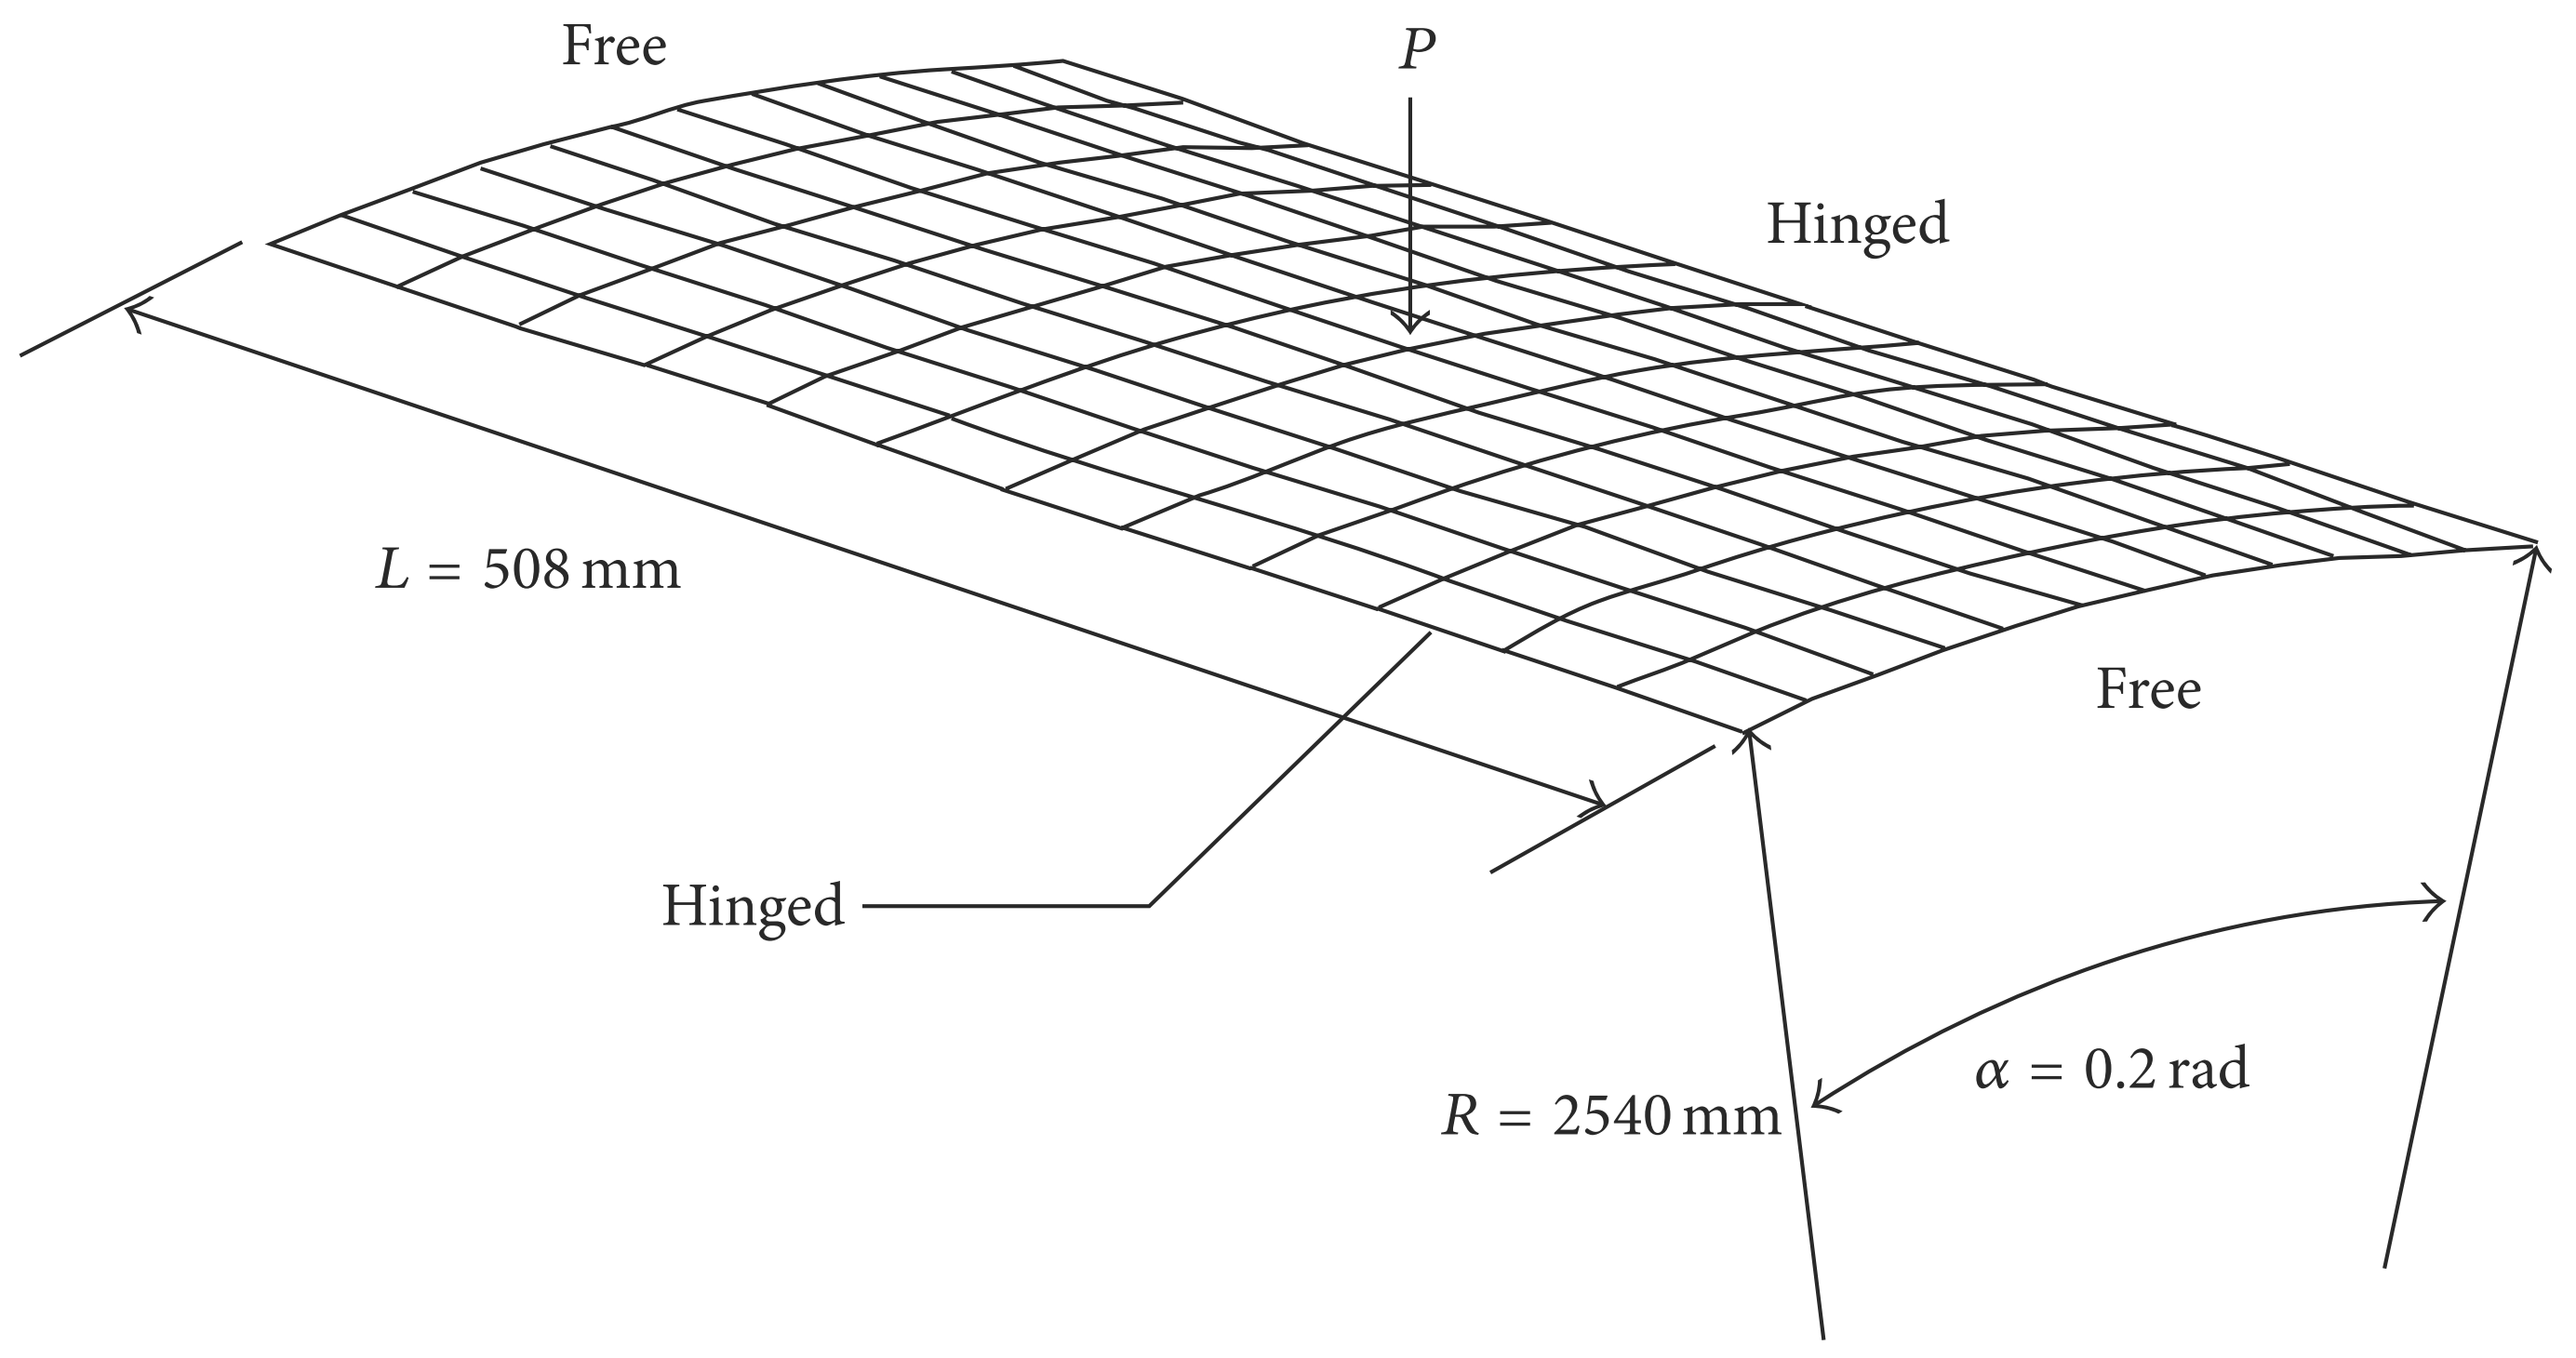
\includegraphics[width=7.3cm]
		{images/hinged_cylindrical_roof.png}}
	\subfloat[Load-displacement curve of hinged cylindrical roof]
	{\label{ref_label2}
		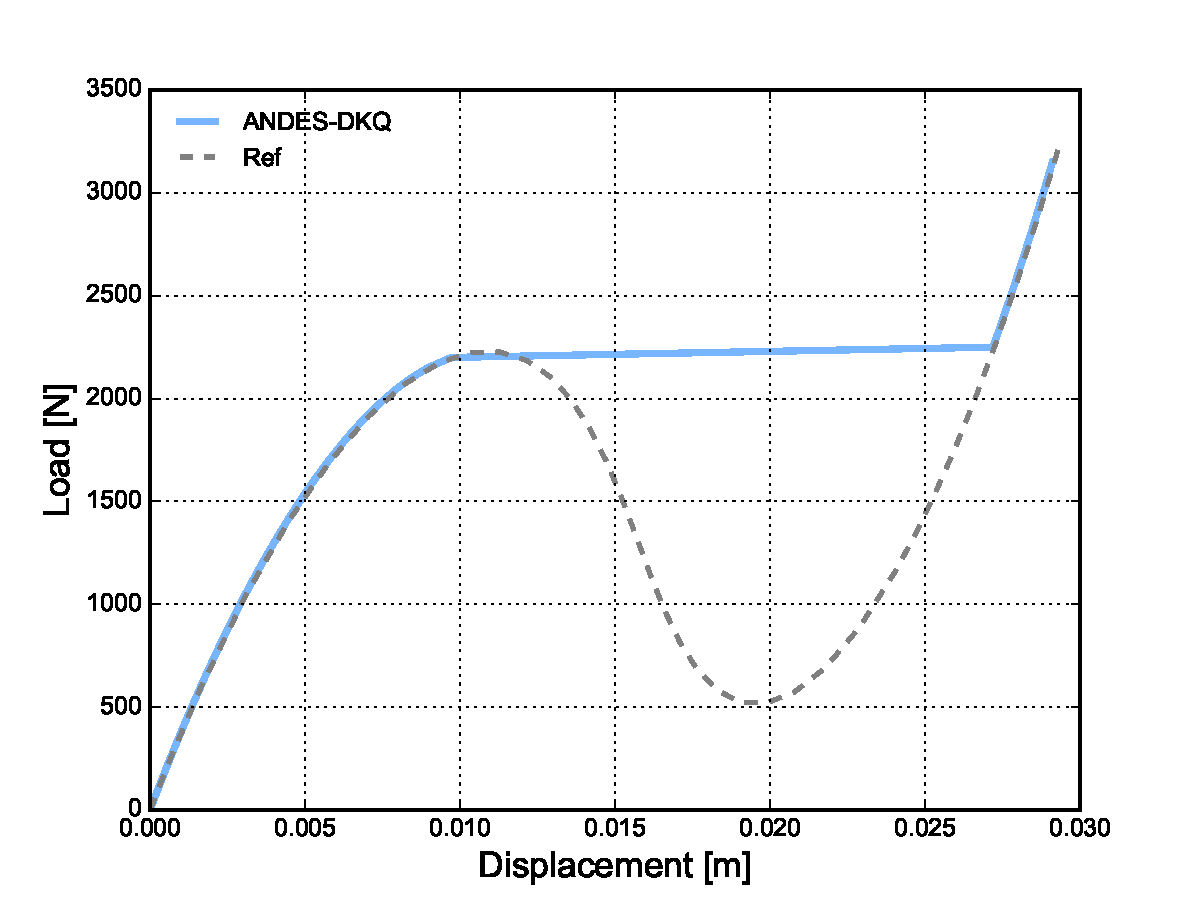
\includegraphics[width=7.3cm]
		{Load_displacement_curve_hinged_cylindrical_roof.pdf}}
	\caption{\label{ref_label_overall}Hinged cylindrical roof validation test}
\end{figure}

 
The load displacement curve plots the equilibrium path for the ANDES-DKQ and DSG elements against the reference path from \cite{Sze2004}. Both elements correctly resolve the entire equilibrium path including both critical points before ending in the structure's snapped-through state.

\newpage
\subsection{Open cylinder pull-out}

The second geometrically non-linear benchmark is the pull-out of an open cylinder with a load $P_{max} = 40\ 000$. The geometry of the cylinder is $L= 10.35,\ R = 4.953$ and $h = 0.094$ while the linear elastic material is characterised by $E = 10.5\times10^6$ and $\nu = 0.3125$. The measured displacement is the vertical deformation $u_z$ at the point of load application.

 
\begin{figure}[H]
	%\centering
	\subfloat[Open cylinder pullout definition \cite{Sze2004}]
	{\label{ref_label1}
		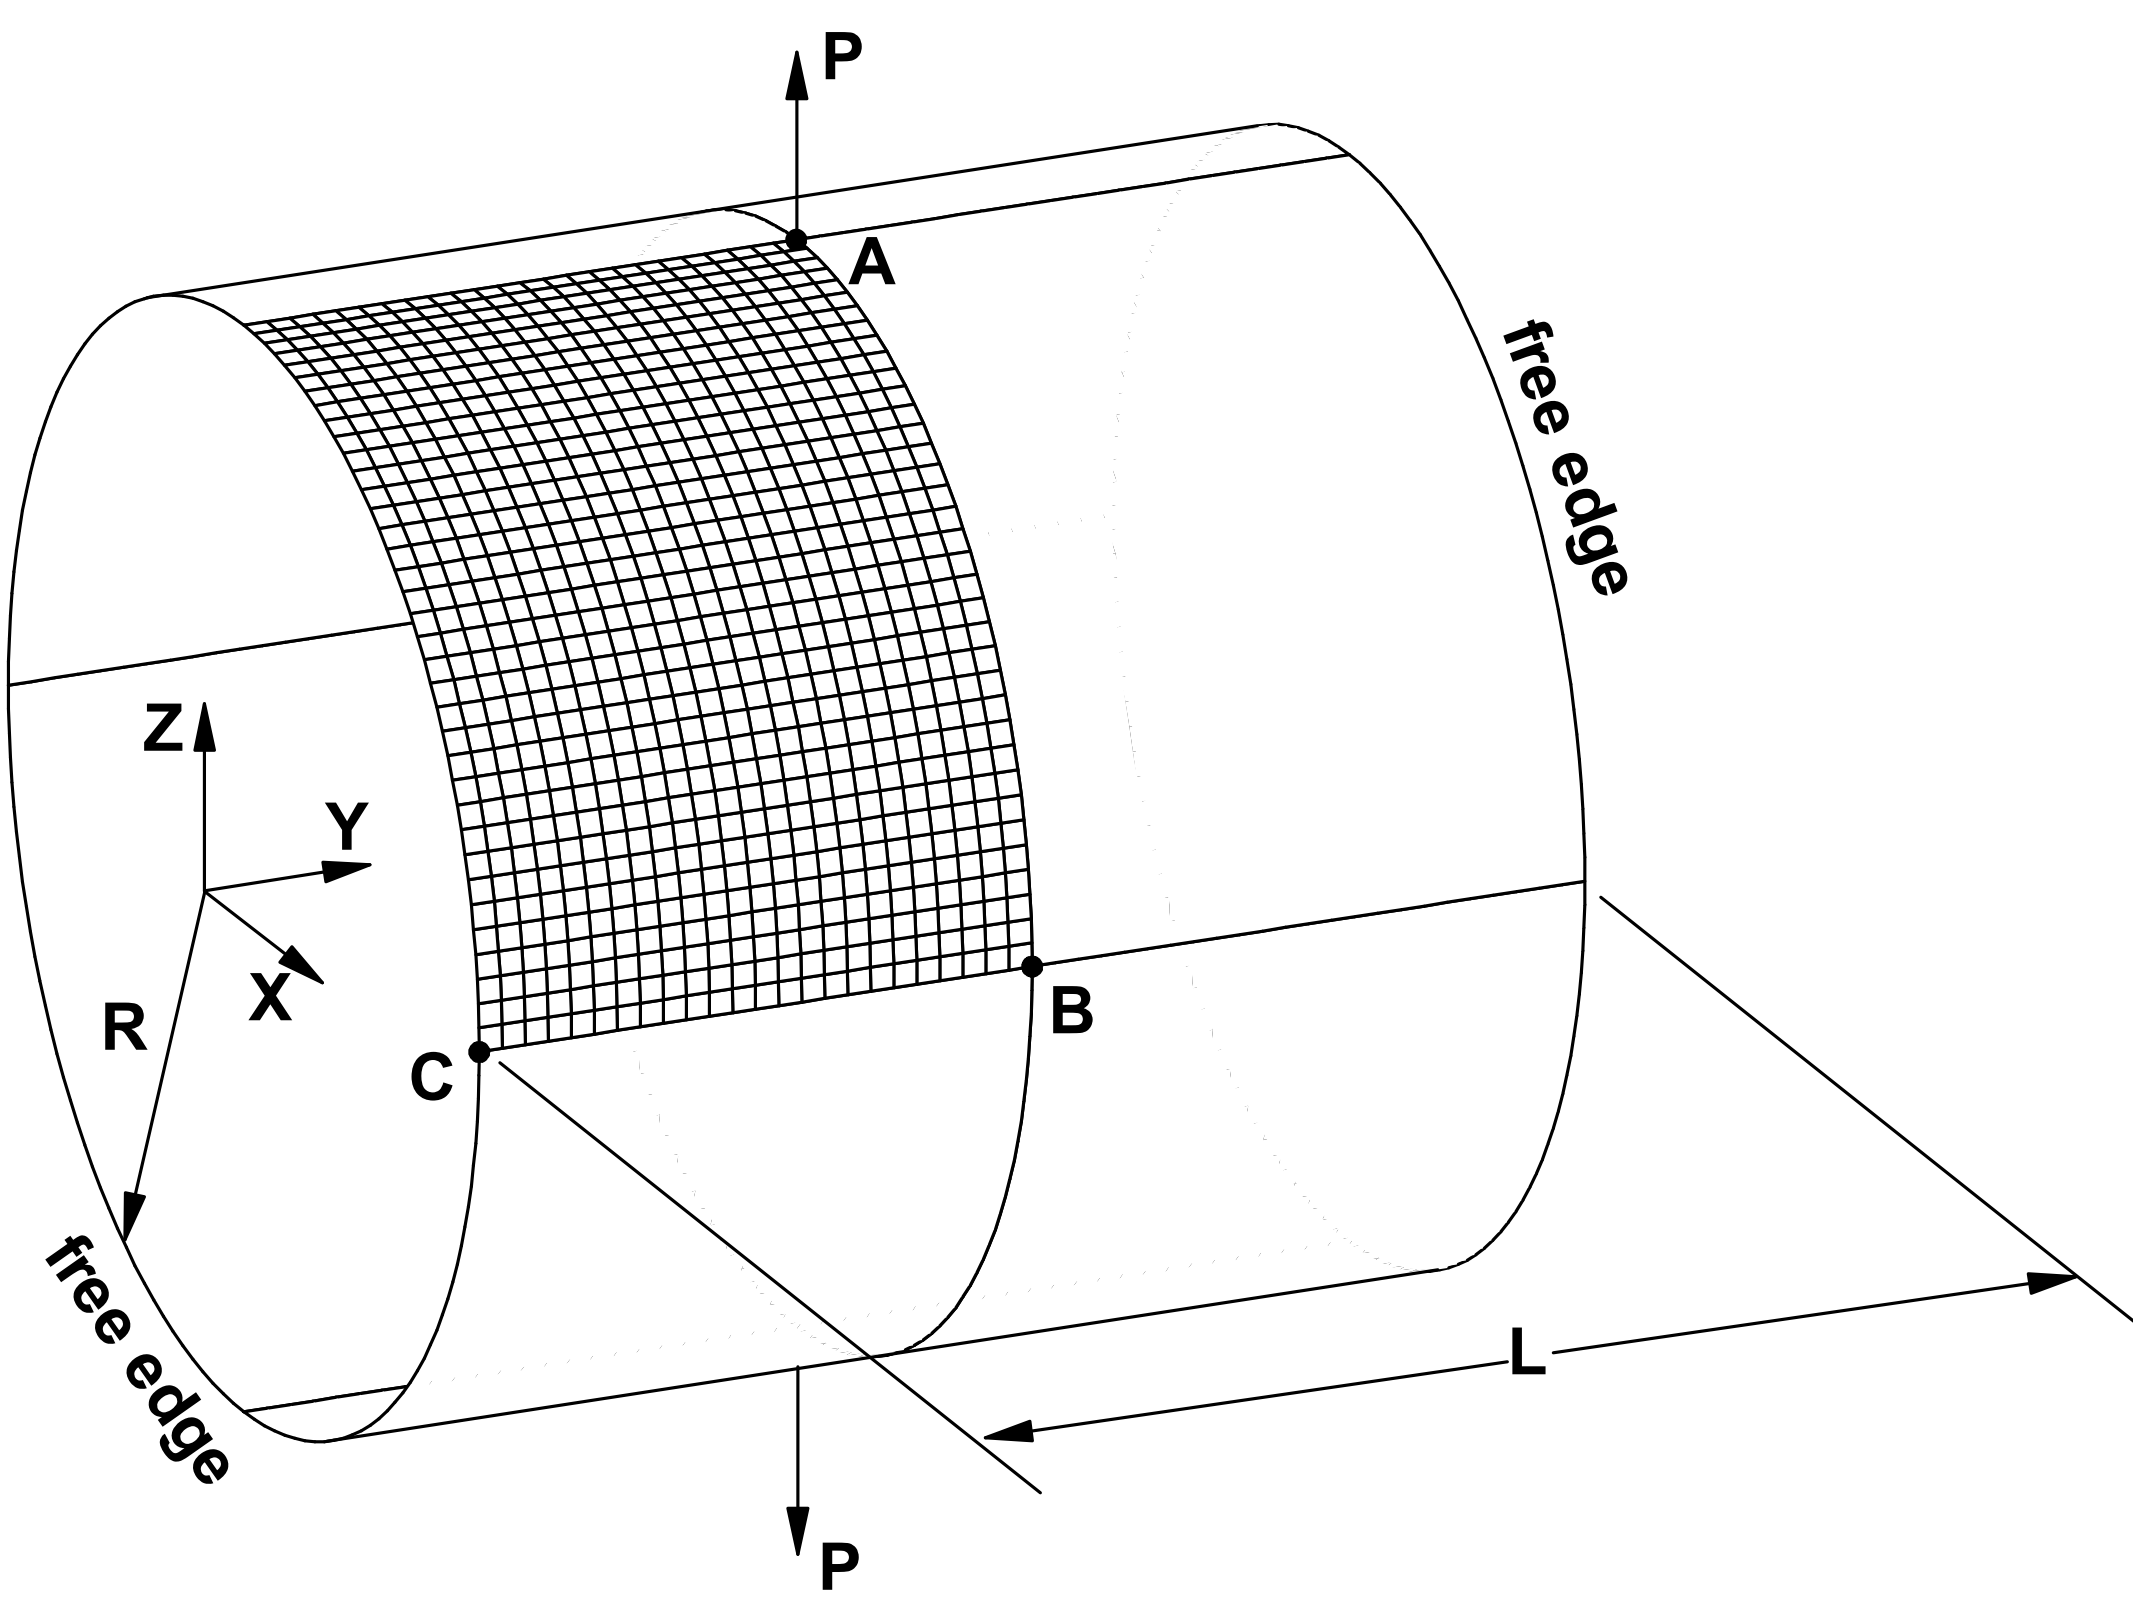
\includegraphics[width=7.3cm]
		{images/opencylinderpullout.png}}
	\subfloat[Load-displacement curve of open cylinder pullout]
	{\label{ref_label2}
		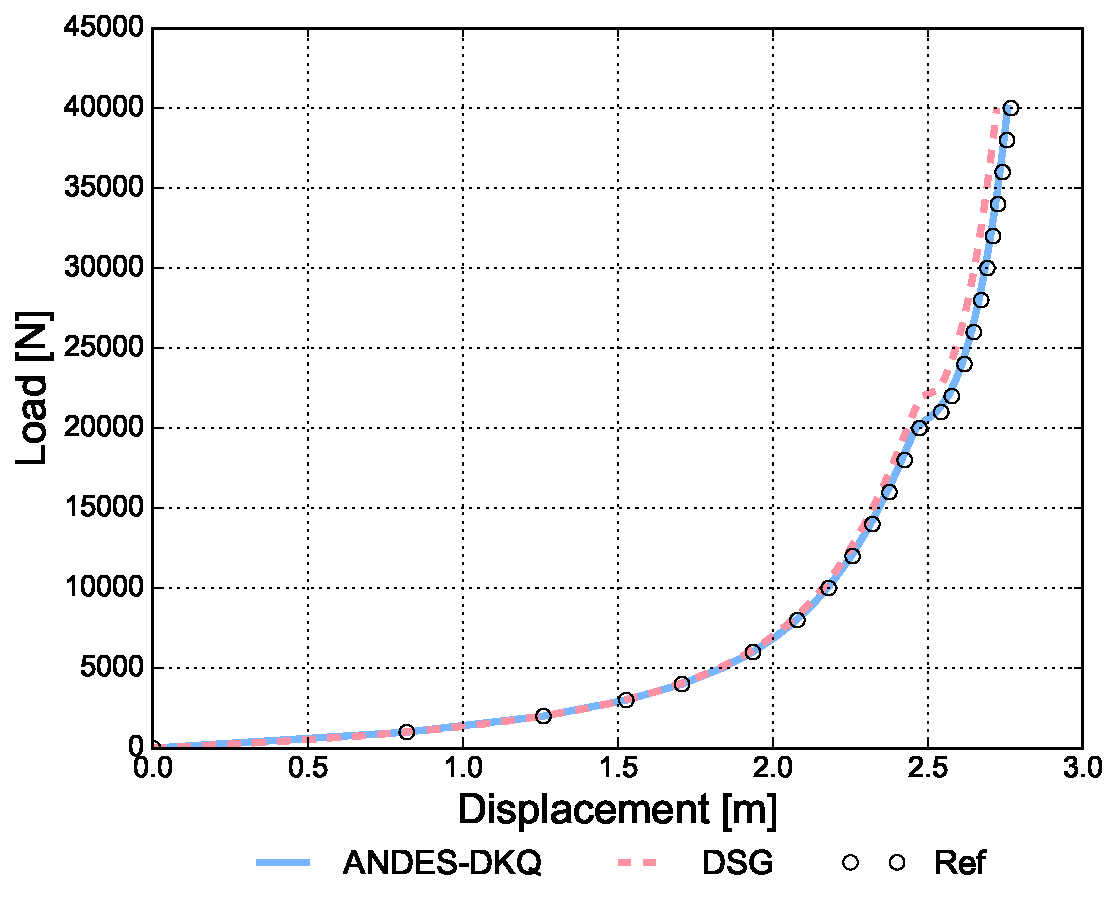
\includegraphics[width=7.3cm]
		{Load_displacement_curve_open_cylinder_pullout.pdf}}
	\caption{\label{ref_label_overall}Open cylinder pull-out validation test}
\end{figure}

 The load-displacement curve above plots the equilibrium path for the ANDES-DKQ and DSG elements against the reference solution \cite{Sze2004}. Both elements closely follow the reference path, which demonstrates the structure gradually activating membrane stiffness before suddenly straightening out and becoming entirely membrane dominated.

\section{Geometrically linear and non-linear dynamic tests}

Dynamic problems introduce inertial effects into the array of phenomena analysed. Combined with the aforementioned co-rotational formulation, it is possible to accurately resolve bodies undergoing large movements over time.

\subsection{Non-linear dynamic shell pendulum}
\label{validation:shell pendulum}
The first dynamic benchmark is a simple shell pendulum allowed to freely rotate along one hinged edge. The initial horizontal configuration of the $1m\times1m\times0.1m$ thick square plate is subject to gravity $g = 9.8\ m/s^2$ acting in the vertical $Z$ direction. The material of the plate is described by $E = 1\times 10^9 Pa,\ \nu = 0.0$ and $\rho = 7850 kg/m^3$. The key result is the vertical displacement component of the free corner node as drawn below.

\begin{figure}[H]
	\centering
	\def\svgwidth{\columnwidth}
	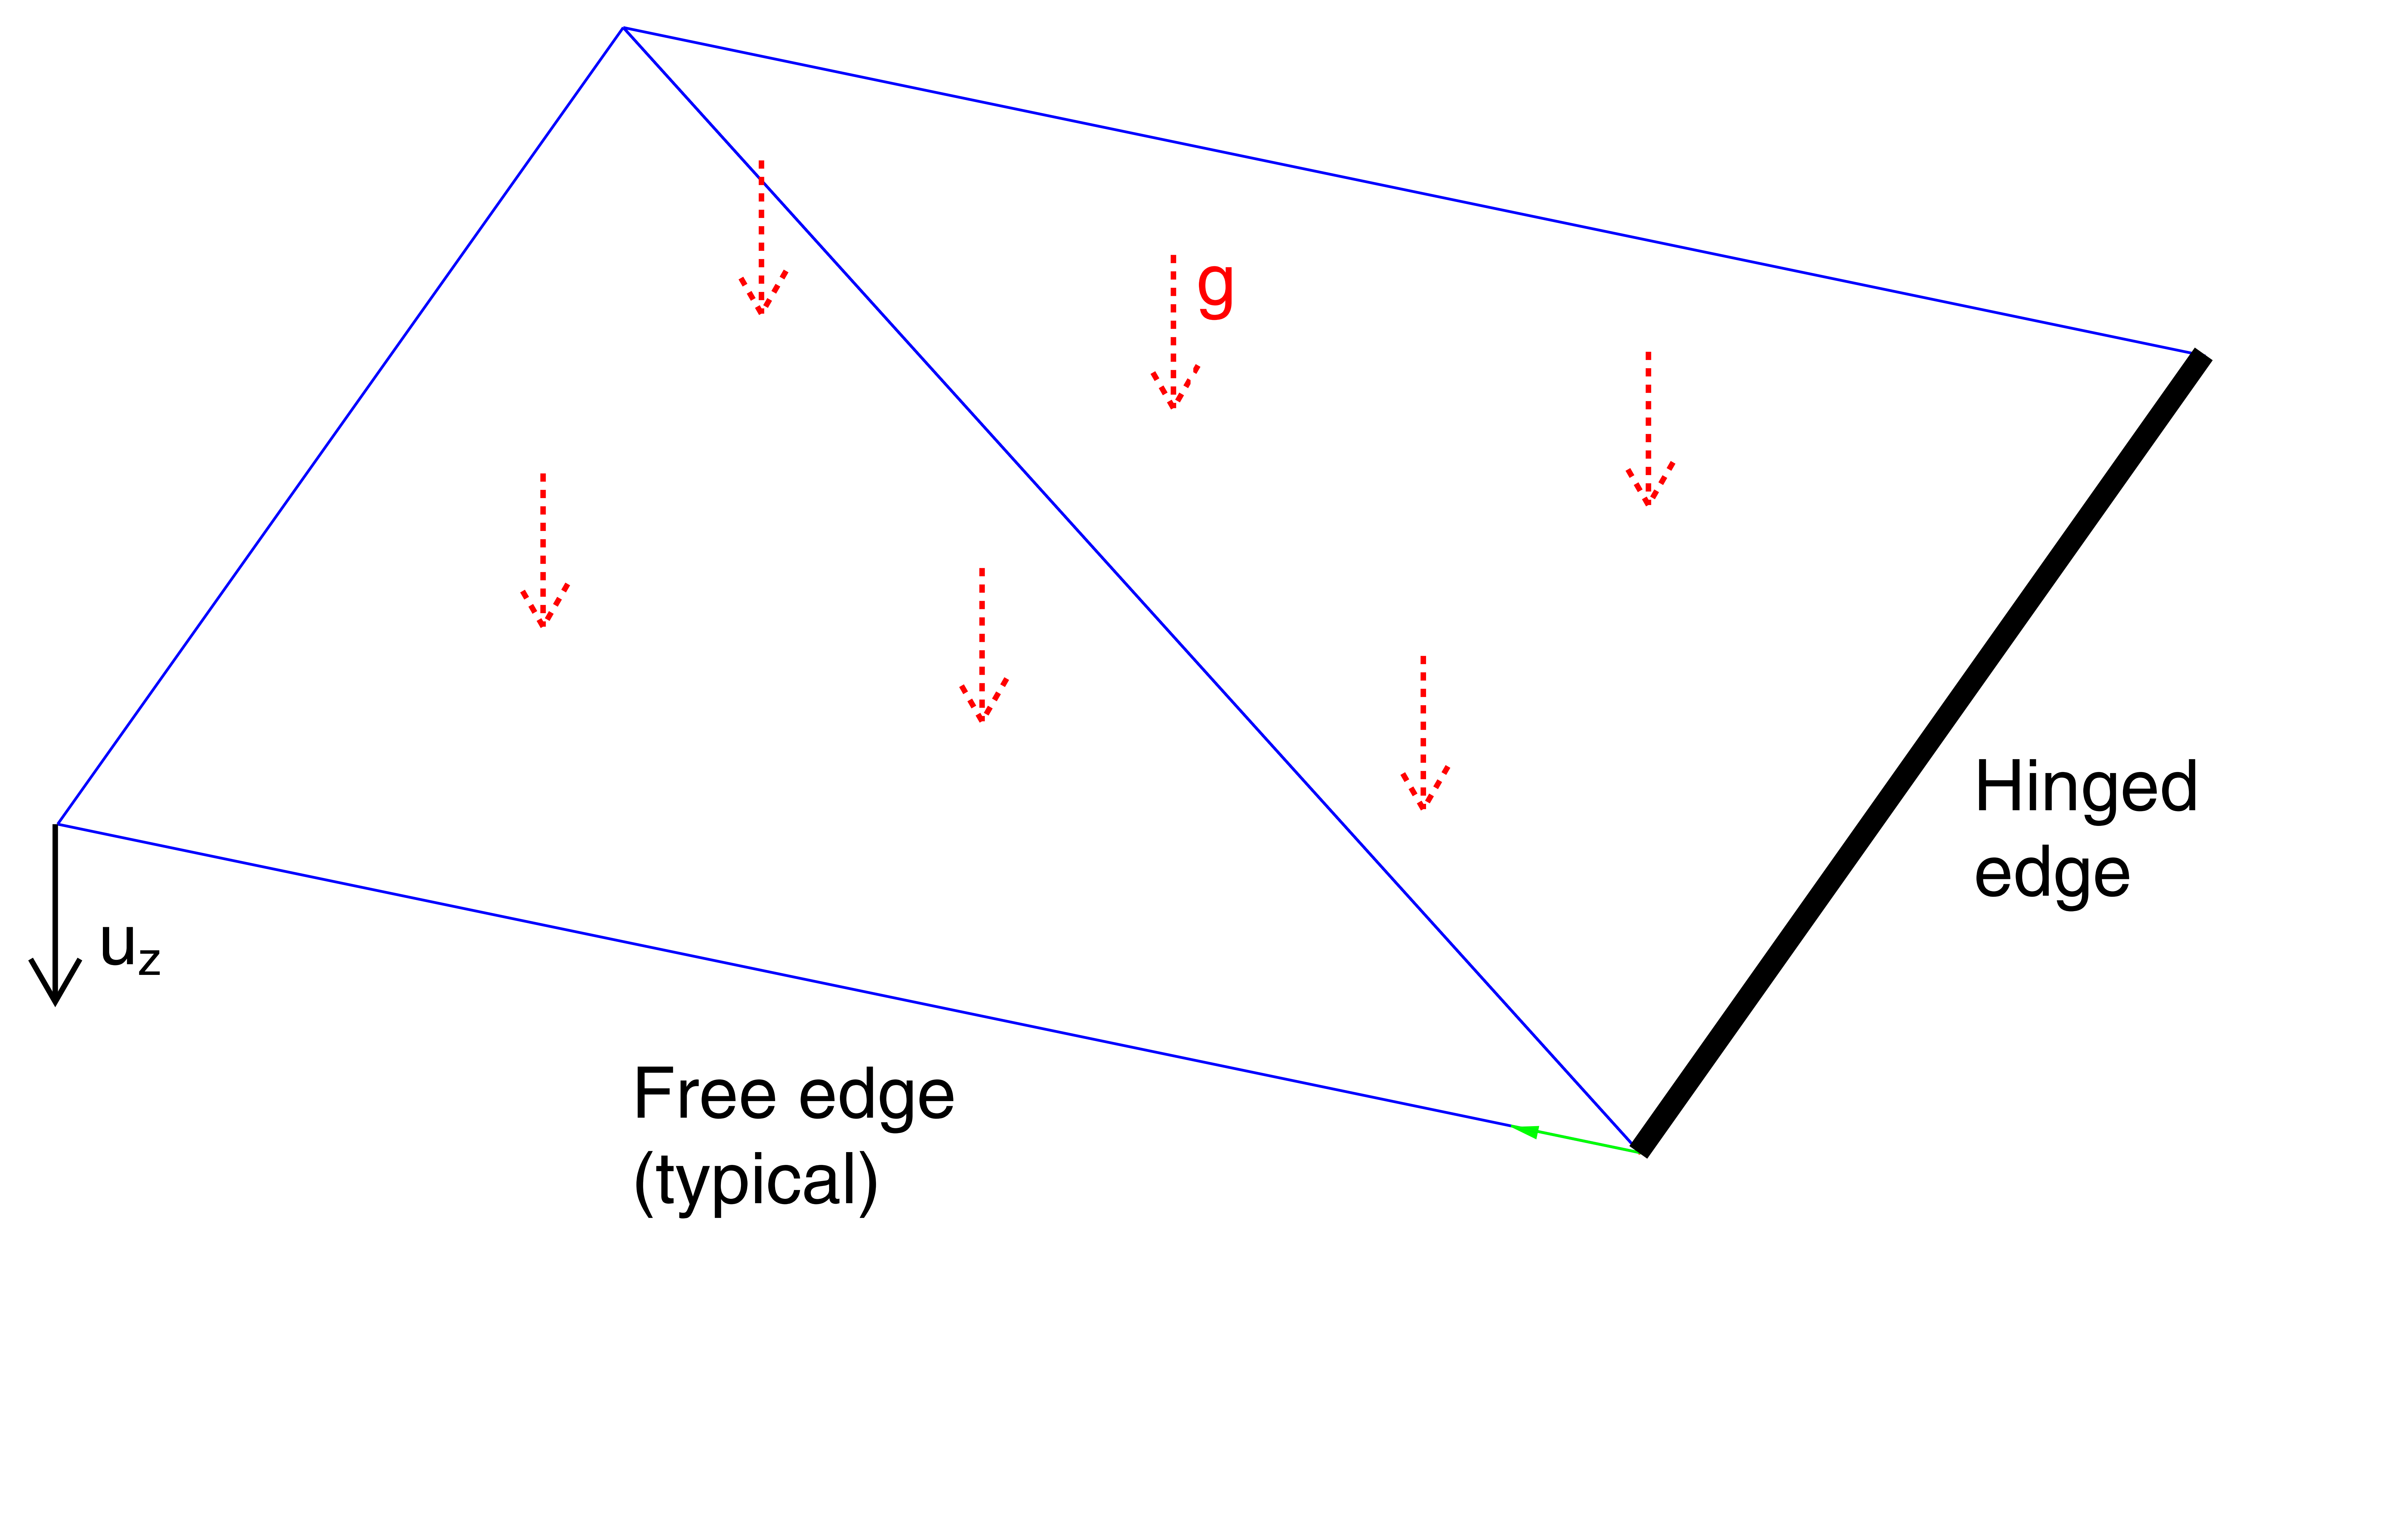
\includegraphics[width=7.3cm]{images/swinging_plate_problem.png}
	\caption{Shell pendulum validation test definition}
\end{figure}
\begin{figure}[H]
	%\centering
	\subfloat[Results using lumped mass matrices]
	{\label{ref_label1}
		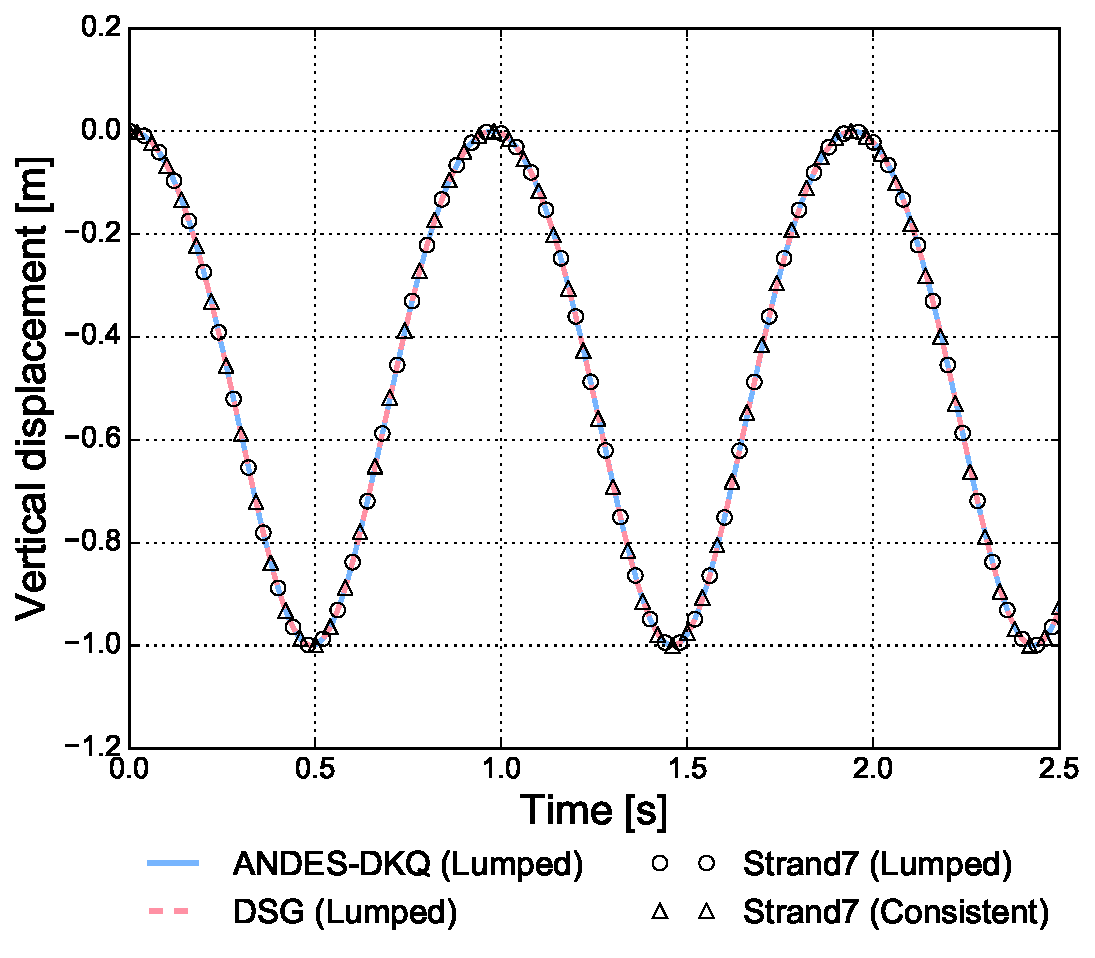
\includegraphics[width=7.3cm]
		{images/shell_pendulum_lumped.pdf}}
	\subfloat[Results using consistent mass matrices]
	{\label{ref_label2}
		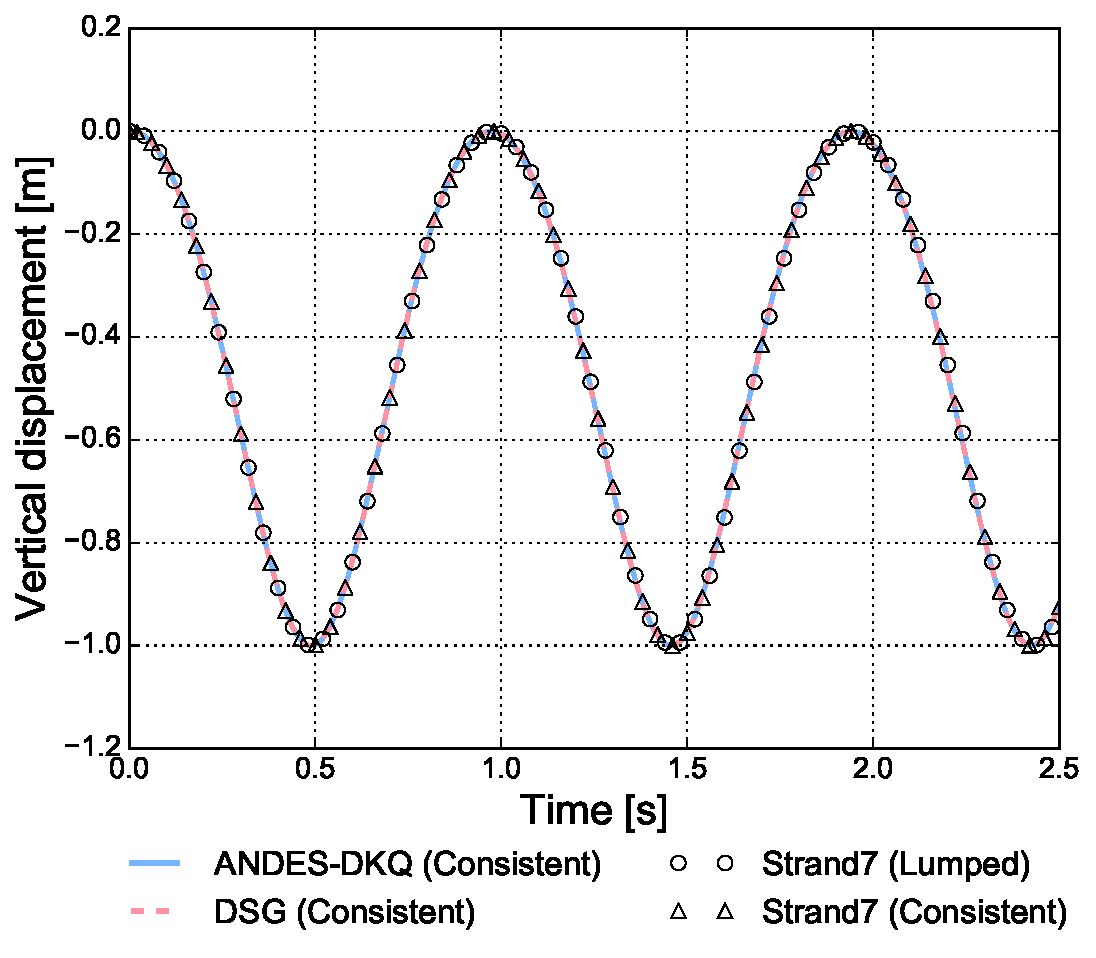
\includegraphics[width=7.3cm]
		{images/shell_pendulum_consistent.pdf}}
	\caption{\label{ref_label_overall}Vertical displacement over time of the shell pendulum validation test}
\end{figure}

The plot of displacement over time demonstrates the ability of both elements to handle large displacements and rotations, agreeing with the reference solution of the existing Kratos quadrilateral shell element. As expected, the minimum vertical displacement of $u_z=-1m$ corresponds to the position of bottom dead centre of the plate, while the maximum vertical displacement of $u_z=0m$ corresponds to a fully horizontal plate orientation

\subsection{Linear dynamic oscillating clamped plate}

The oscillating clamped plate benchmark subjects a clamped cantilever square plate $2m\times2m\times0.1m$ thick to a uniform globally oriented surface pressure of $P_z = -0.25 Pa$. The plate material is linear elastic characterised by $E = 1\times 10^6 Pa,\ \nu = 0.0$ and $\rho = 7850 kg/m^3$. The key result is the vertical displacement component of the free corner node as illustrated below.

\begin{figure}[H]
	\centering
	\def\svgwidth{\columnwidth}
	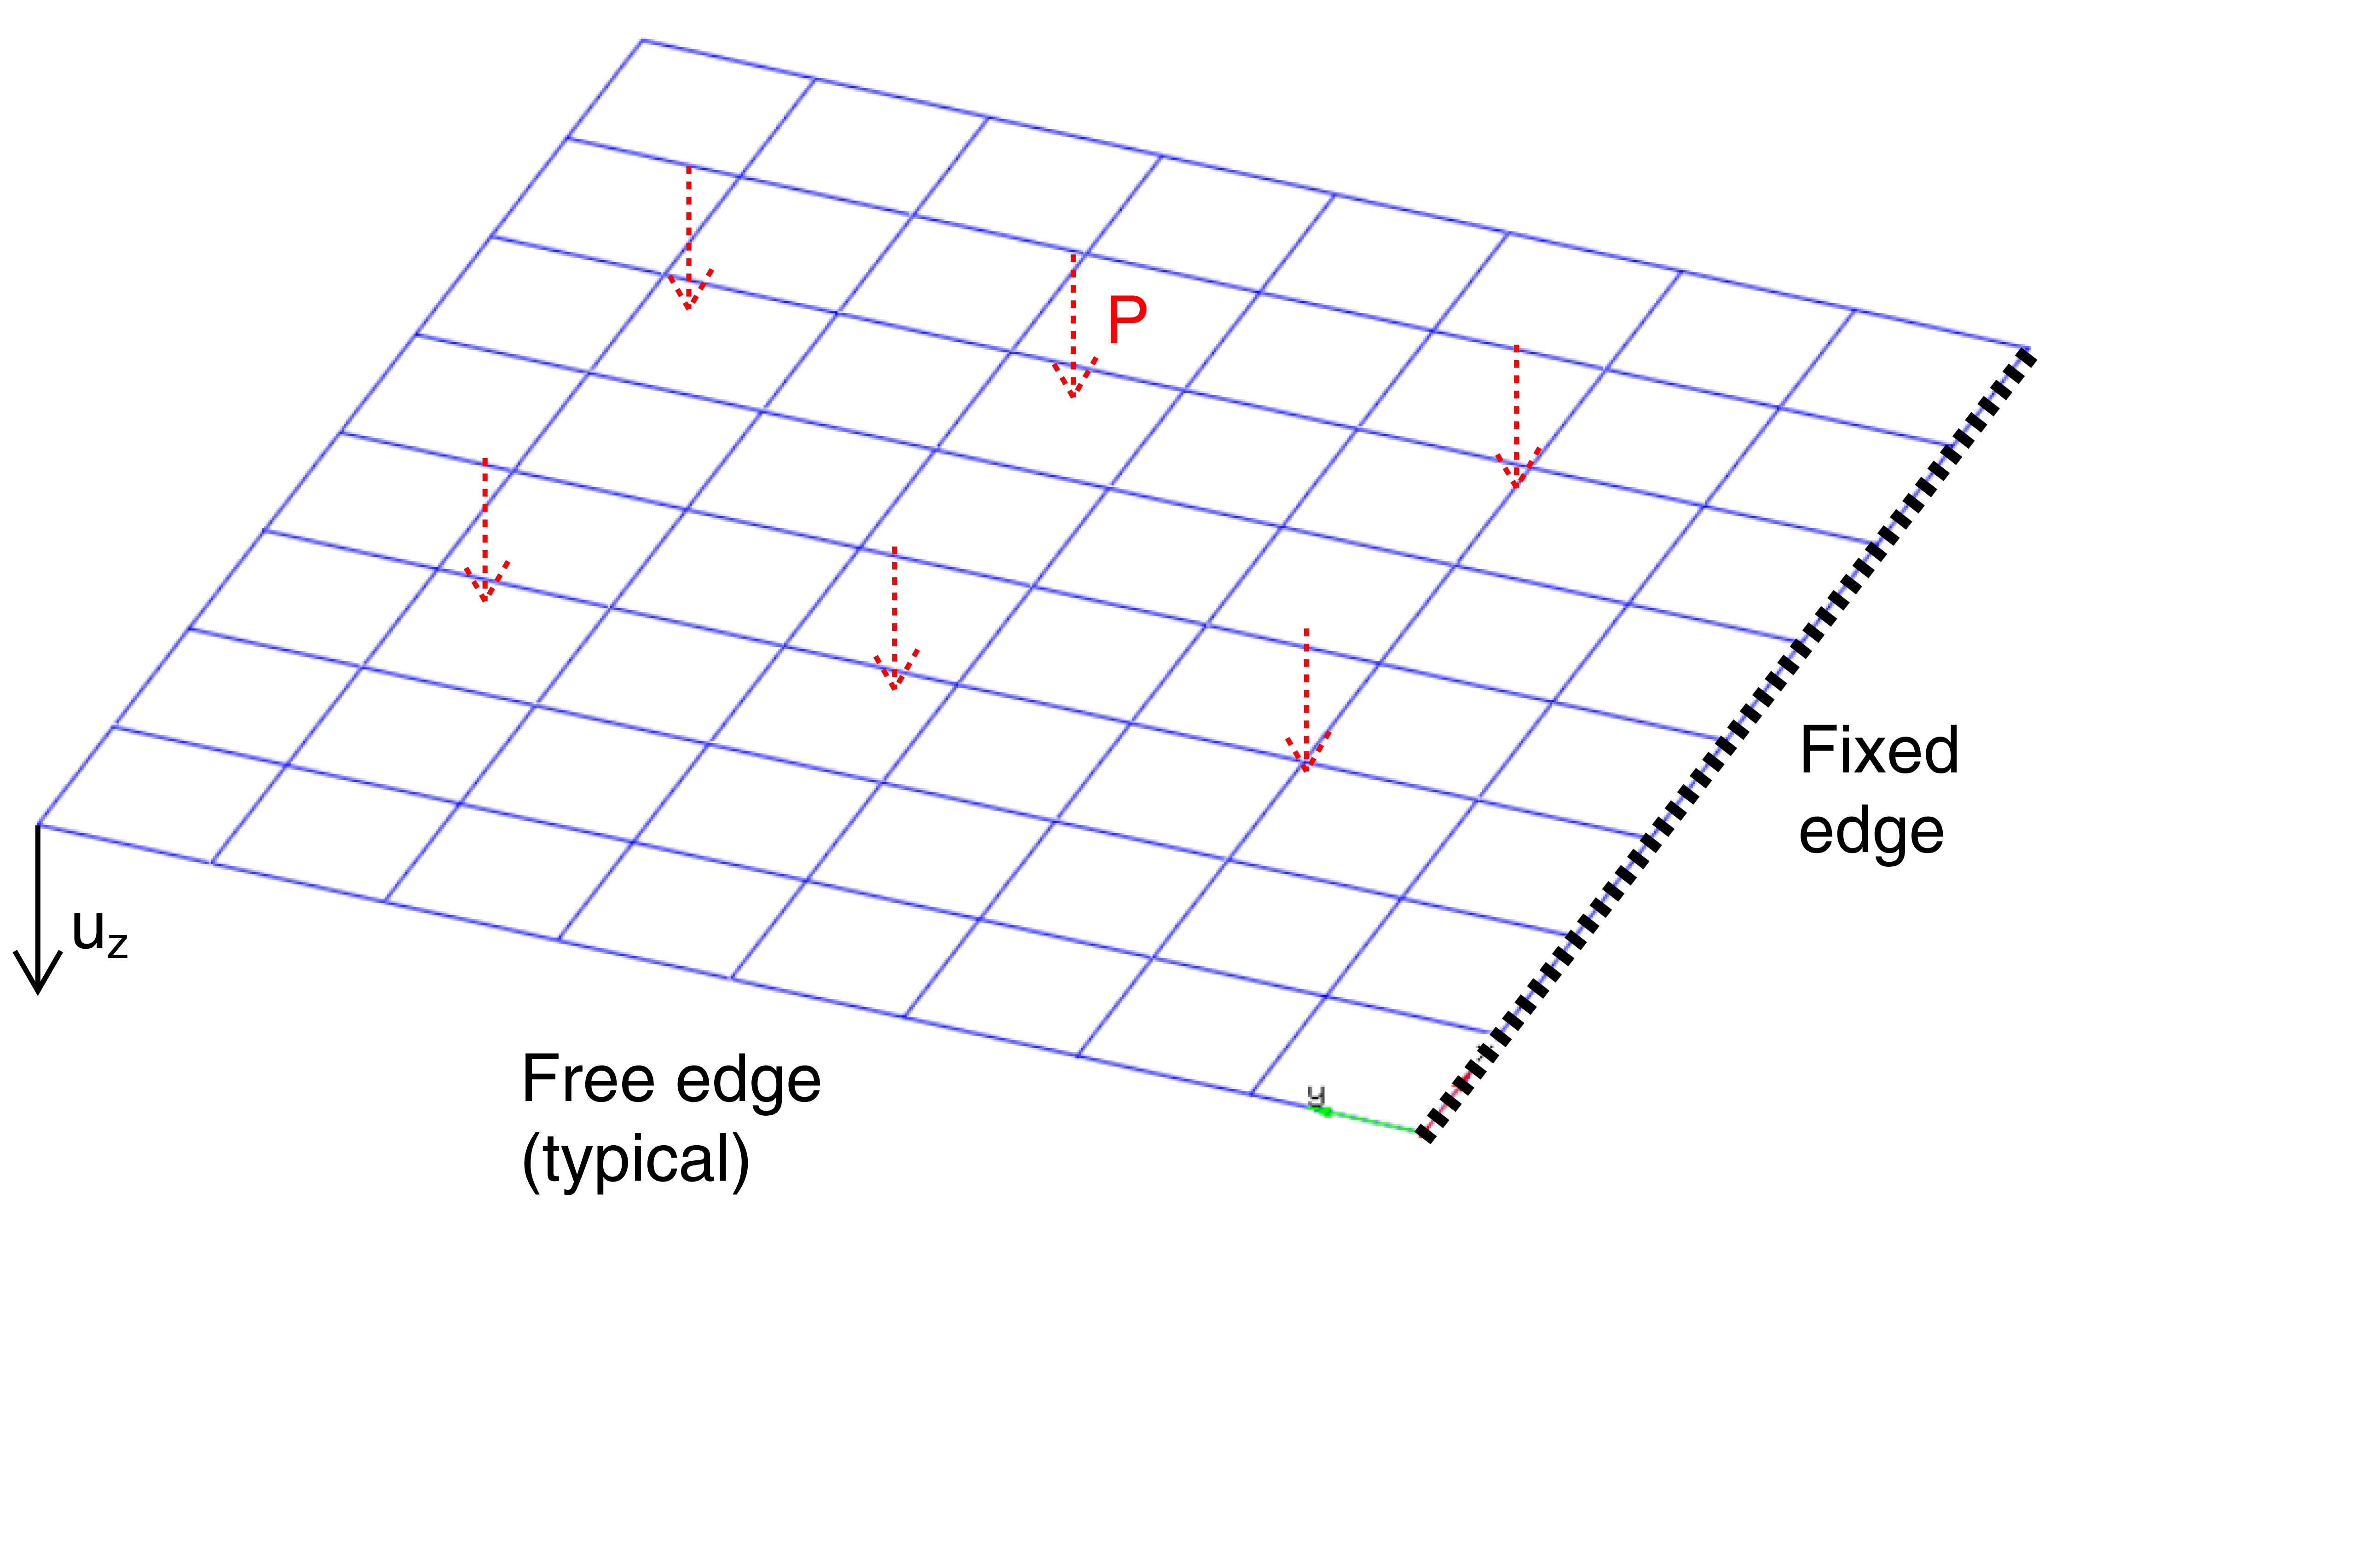
\includegraphics[width=7.3cm]{images/quad_bend_problem.png}
	\caption{Oscillating clamped plate validation test definition}
\end{figure}
\begin{figure}[H]
	%\centering
	\subfloat[Results using lumped mass matrices]
	{\label{ref_label1}
		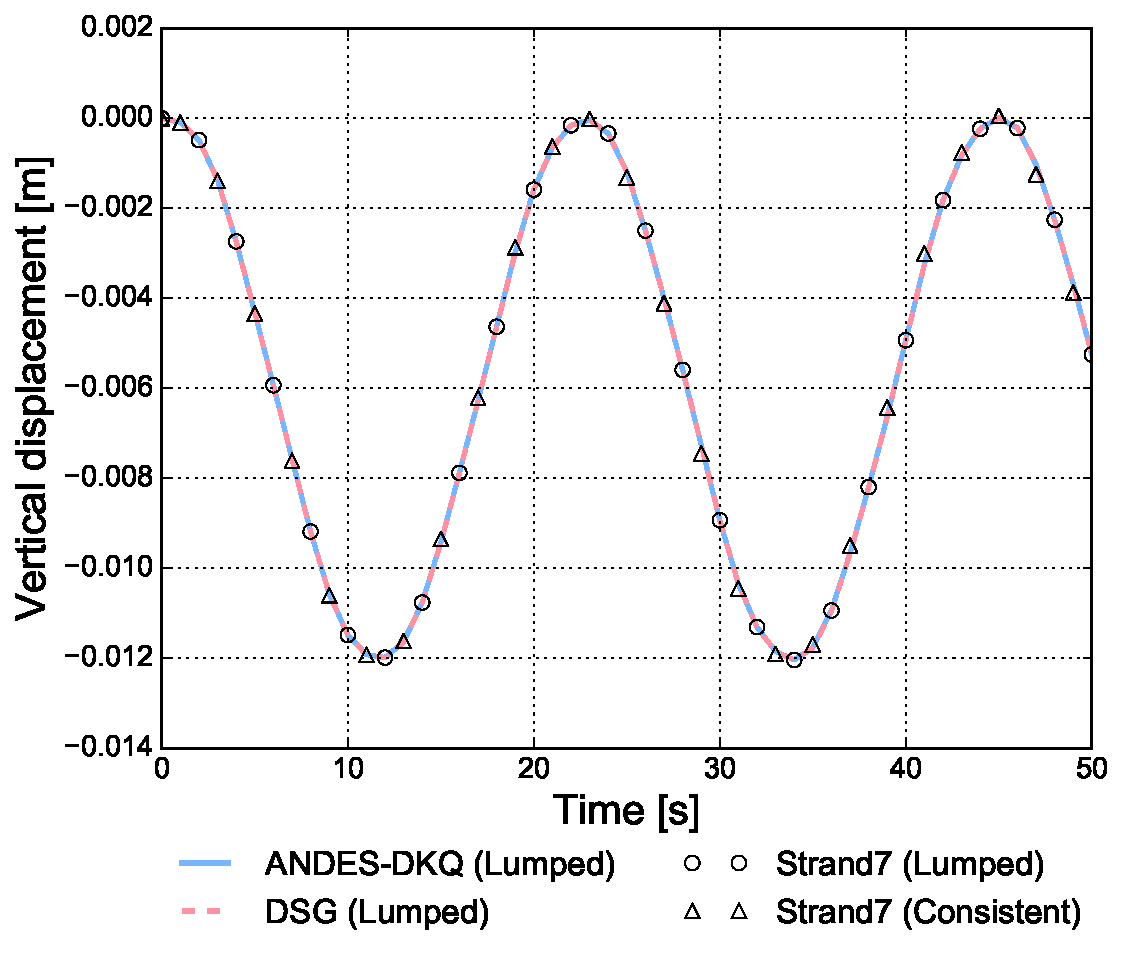
\includegraphics[width=7.3cm]
		{images/oscillating_plate_lumped.pdf}}
	\subfloat[Results using consistent mass matrices]
	{\label{ref_label2}
		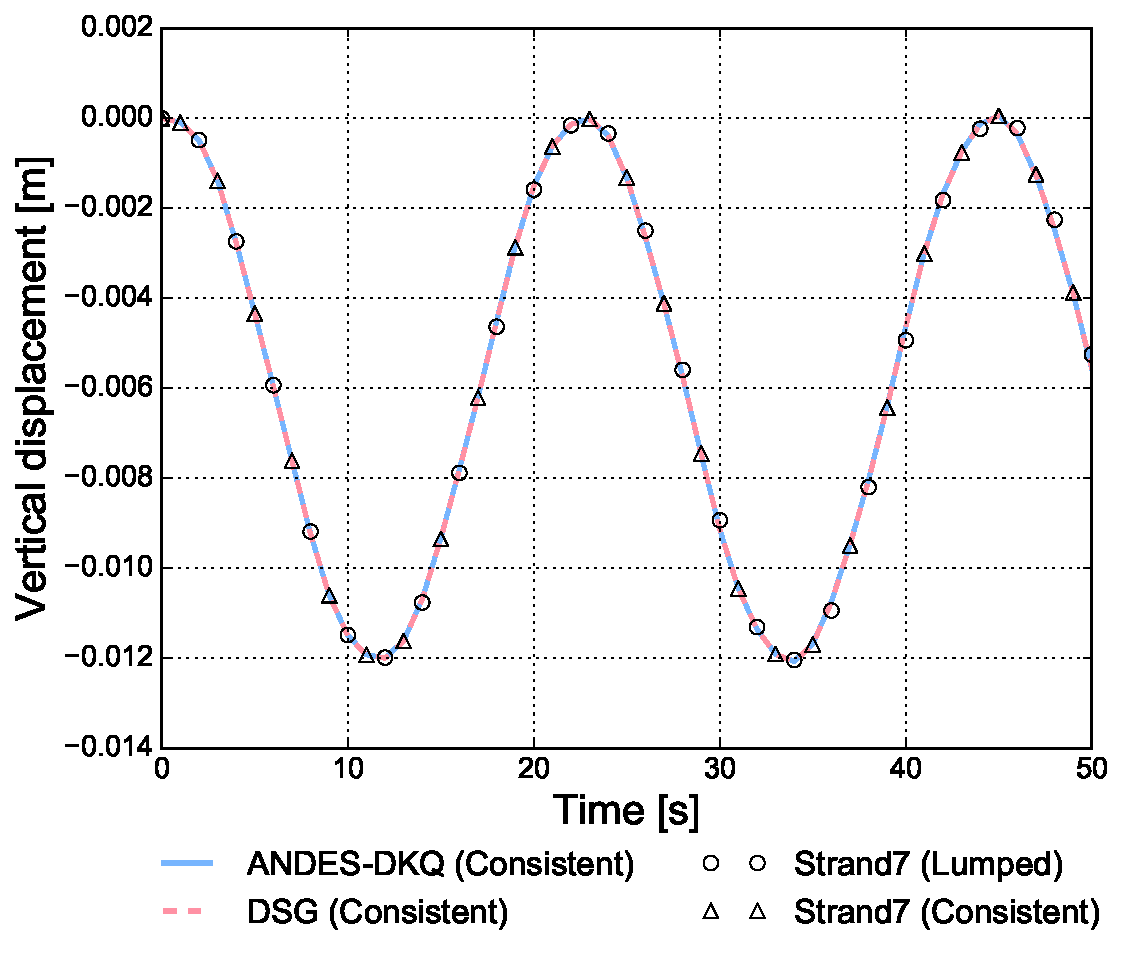
\includegraphics[width=7.3cm]
		{images/oscillating_plate_consistent.pdf}}
	\caption{\label{ref_label_overall}Vertical displacement over time of the oscillating clamped plate validation test}
\end{figure}

 The plot of vertical displacement over time demonstrates both elements agree with the reference solution, which is the existing Kratos quadrilateral element. The overall results correctly correspond to structural dynamics theory by oscillating with the base natural frequency about the static displacement of $u_z=-0.006m$.

\section{Quantity recovery tests}

Although displacements are the primary solution variables of a finite element analysis, recovered quantities, such as strains, stresses and force resultants are often more critical to the success or failure of a system. The following tests validate the implemented elements ability to correctly recovery these quantities.

\subsection{Simply supported dome with oculus under self weight}
\label{subsection:dome_test}

A simply supported dome with an oculus under self weight is considered to evaluate the membrane results of the elements. The hemi-spherical dome is defined by the following parameters: $R = 5m,\ h = 0.01m,\ \rho = 7850 kg/m^3,\ g = 9.81m/s^2,\ E = 2 \times 10^{11} Pa,\ \nu = 0.3$. The 20 degree opening has no edge loading. Appendix \ref{app:Analytical membrane analysis of dome} derives the analytical formulae which form the reference solution for both force resultants, while an analysis of the problem with ANSYS provides the Von Mises stress reference solution.

\begin{figure}[H]
	%\centering
	\subfloat[Circumferential shell force over meridian angle]
	{\label{ref_label1}
		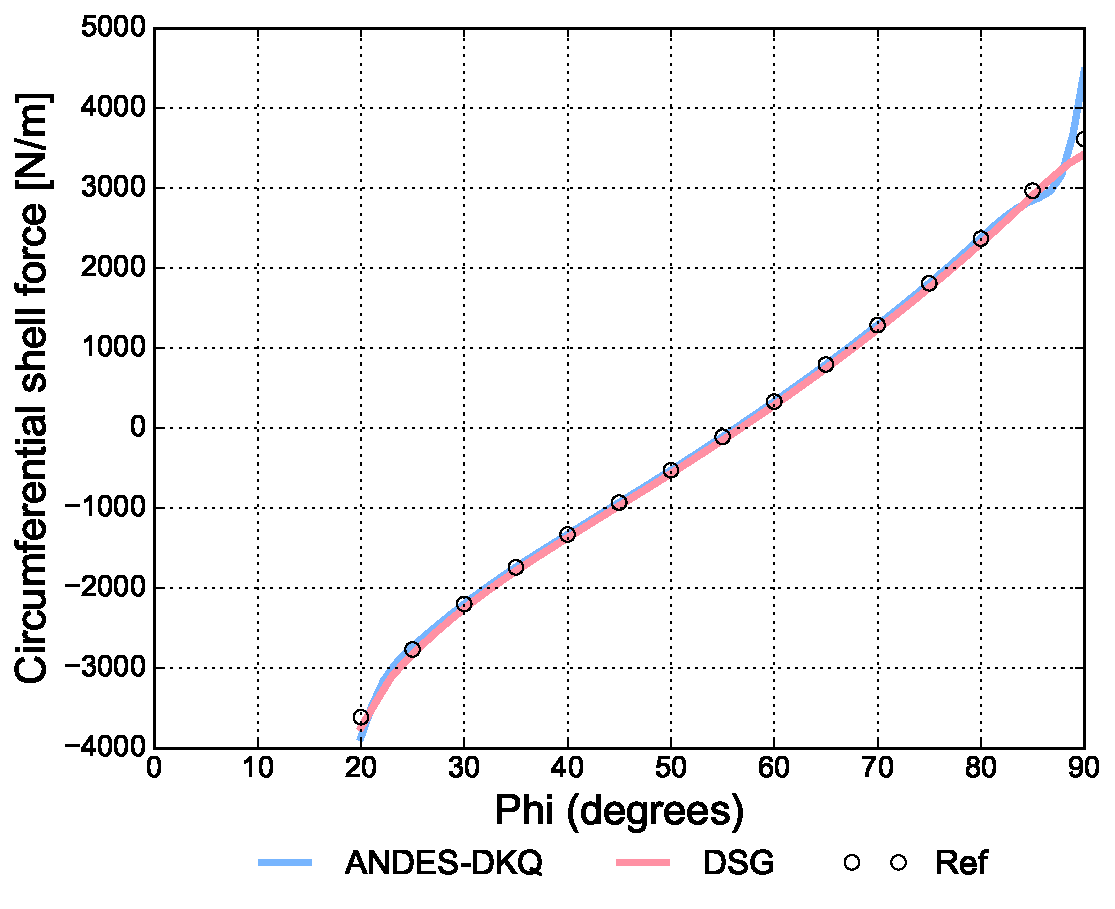
\includegraphics[width=7.3cm]
		{images/Simply_support_dome_n_theta.pdf}}
	\subfloat[Meridional shell force over meridian angle]
	{\label{ref_label2}
		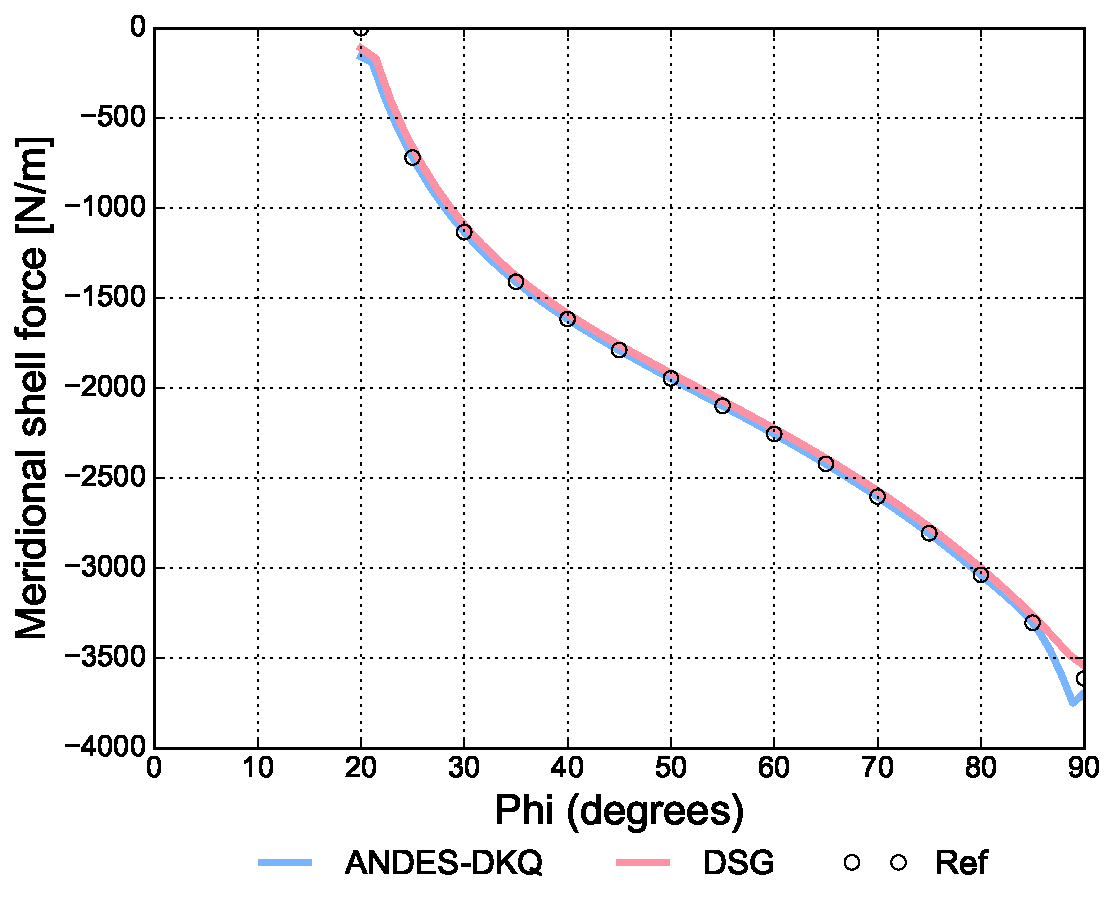
\includegraphics[width=7.3cm]
		{images/Simply_support_dome_n_phi.pdf}}
	\\
		\subfloat[Mid-plane Von Mises stress over meridian angle]
	{\label{ref_label1}
		\includegraphics[width=7.3cm]
		{images/Simply_support_dome_von_mises.pdf}}
	\subfloat[Mid-plane Von Mises plot of the reference ANSYS solution]
	{\label{ref_label2}
		\includegraphics[width=7.3cm]
		{images/simply_support_dome_ansys_vm_plot.png}}
	\\
	\subfloat[Mid-plane Von Mises plot of the ANDES solution]
	{\label{ref_label1}
		\includegraphics[width=7.3cm]
		{images/simply_support_dome_andes_vm_plot.png}}
	\subfloat[Mid-plane Von Mises plot of the DSG solution]
	{\label{ref_label2}
		\includegraphics[width=7.3cm]
		{images/simply_support_dome_dsg_vm_plot.png}}
	\caption{\label{Shell_force_dome_benchmark_shell_force}Results of the simply supported dome validation test}
\end{figure}

The results of both elements for circumferential and meridional shell forces demonstrate excellent agreement with the analytical membrane analysis. Minor deviations occur at both ends of the dome due to the strict assumptions of the analytical membrane theory and mesh effects. The mid-surface Von Mises stress results also agree with the ANSYS solution quite closely, with the ANDES-DKQ slightly out-performing the DSG element. The contour plots (with all limits set to $[1.4\times 10^5,\ 7.5\times10^5]$) further exhibit the similarities between the three solution methods.
%limits all set to [1.4e5, 7.5e5] !!!!!!
\subsection{Navier supported plate under sinusoidal load}
\label{validation:navier plate under sinusoidal load}
A Navier supported square plate subject to a sinusoidal load is considered to examine the bending stress results of the ANDES-DKQ element. A 3-parameter analytical solution forms the reference for this problem \cite{reddy2004mechanics}. 

\begin{figure}[H]
	\centering
	\def\svgwidth{\columnwidth}
	\includegraphics[width=7.3cm]{images/navier_plate_def.png}
	\caption{Definition of the Navier supported plate validation test \cite{reddy2004mechanics}}
	\label{validation:pic navier plate}
\end{figure}

Due to symmetry, one quarter of a $a = 200,\ b = 200,\ h = 10$ square plate of linear isotropic material $E = 2\times 10^{11}$ and $\nu = 0.3$ is modelled and subject to a spatially varying transverse pressure of $q = -1\times 10^7 sin(\frac{x\pi}{200})sin(\frac{y\pi}{200})$. The following graphs plot quantities along a path from $x=0$ to $x=100$ at $y=100$.

\begin{figure}[H]
	%\centering
	\subfloat[Normal stress (XX) over X coordinate]
	{\label{ref_label1}
		\includegraphics[width=7.3cm]
		{images/navier_plate_quad_s_xx_bot.pdf}}
	\subfloat[Normal stress (YY) over X coordinate]
	{\label{ref_label2}
		\includegraphics[width=7.3cm]
		{images/navier_plate_quad_s_yy_bot.pdf}}
	\\
	\subfloat[Shear stress (XY) over X coordinate]
	{\label{ref_label1}
		\includegraphics[width=7.3cm]
		{images/navier_plate_quad_s_xy_bot.pdf}}
	\subfloat[Von Mises stress over X coordinate]
	{\label{ref_label2}
		\includegraphics[width=7.3cm]
		{images/navier_plate_quad_s_vm_bot.pdf}}
	\caption{\label{Navier_quad_s_xx_yy}Stresses (bottom surface) of the Navier supported plate under sinusoidal load}
\end{figure}

The above figures demonstrate exemplary alignment between the analytical solution and the ANDES-DKQ element across all stresses considered.

\subsection{Navier supported plate under uniformly distributed load}
\label{validation:DSG navier unifom}

A Navier supported square plate subject to a uniformly distributed load is considered to examine the bending stress results of the DSG element. An ANSYS analysis forms the reference for this problem. The problem setup is identical to the preceding test with the exception of a uniformly distributed transverse pressure $q = -1\times 10^{11}$ and "hard" supports along the edges ($\phi_x = 0$ on edges parallel to y-axis, $\phi_y = 0$ on edges parallel to x-axis).

Graphs plotted along an X coordinate follow the same path as the preceding tests. Graphs plotted along a Y coordinate run from $y = 0$ to $y = 100$ with $x = 100$, while graphs plotted along a diagonal distance run from $x=y=0$ to $x=y=100$.
%
%\begin{figure}[h!]
%	\centering
%	\includegraphics[width=14cm]{images/navier_thick_tri_paths}
%	\caption{Paths for results: Red = X path and Green = Y path}
%	\label{fig:navierthicktripaths}
%\end{figure}
%
%\newpage

\begin{figure}[h!]
	%\centering
	\subfloat[Normal stress (XX) over X coordinate]
	{\label{ref_label1}
		\includegraphics[width=7.3cm]
		{images/navier_plate_tri_s_xx.pdf}}
	\subfloat[Normal stress (YY) over X coordinate]
	{\label{ref_label2}
		\includegraphics[width=7.3cm]
		{images/navier_plate_tri_s_yy.pdf}}
	\\
	\subfloat[In plane shear stress (XY) over plate diagonal]
	{\label{ref_label1}
		\includegraphics[width=7.3cm]
		{images/navier_plate_tri_s_xy.pdf}}
	\subfloat[Transverse shear stress (XZ) over X coordinate]
	{\label{ref_label1}
		\includegraphics[width=7.3cm]
		{images/navier_plate_tri_s_xz.pdf}}
	\\
	\subfloat[Transverse shear stress (YZ) over Y coordinate]
	{\label{ref_label1}
		\includegraphics[width=7.3cm]
		{images/navier_plate_tri_s_yz.pdf}}
	\subfloat[Von Mises stress over plate diagonal]
	{\label{ref_label2}
		\includegraphics[width=7.3cm]
		{images/navier_plate_tri_vm.pdf}}
	\caption{\label{Navier_tri_s_xx_yy}Stresses of the Navier supported plate under uniformly distributed load}
\end{figure}

The DSG element shows good agreement with the ANSYS results across all stress quantities considered. The transverse shear stress results have additional result cases of the mesh rotated 90 degrees and an unstructured mesh of similar element size to evaluate if the DSG nodal numbering dependency affects the results. One notes that $\sigma_{yz}$ of the DSG result is essentially the same as $\sigma_{xz}$ of the DSG mesh rotated 90 degrees, as is the case of the reverse too. Furthermore, the unstructured mesh results appear to generally follow the ANSYS results regardless. Thus, it is suspected that the DSG nodal ordering may be affecting the transverse shear stress accuracy, although acceptable accuracy is still achieved when one considers that derived quantities are generally less accurate than displacements.

\section{Composite tests}

The extension of both shell elements to handle composite laminates requires its own validation across the range of tests considered for isotropic shells. The following tests consider the performance of both elements in cases which all employ composite materials. As per the preceding isotropic element tests, cases across linear/non-linear statics, linear/non-linear dynamics, and quantity recovery are examined.

\subsection{Composite linear statics: composite barrel vault}
\label{validation:composite barrel vault}
The composite barrel vault is an extension of the Scordelis-Lo roof obstacle course test to composite materials \cite{reddy2004mechanics}. Corresponding to the following figure, the problem is defined with: $\alpha = 40^{\circ},\ R = 300,\ a = 600$ and $q = 0.625$. The reference quantity is the vertical displacement at the centre of the roof (point A).

\begin{figure}[H]
	\centering
	\def\svgwidth{\columnwidth}
	\includegraphics[width=7.3cm]{images/composite_barrel_vault_def.png}
	\caption{Definition of the composite barrel vault validation test \cite{reddy2004mechanics}}
\end{figure}

The composite material is considered with cross-ply [0/90/0/90...] and angle-ply [-45/45/-45/45/...] lamina stacking arrangements, with each ply having the following material properties: $E_1 = 25 E_2,\ E_2 = 1.2 \times 10^5,\ G_{12} = G_{13} = 0.5 E_2,\ G_{23} = 0.2 E_2$ and $\nu_{12} = 0.25$. Furthermore, the tests are carried out over slenderness ratios of $S = \frac{R}{h} = 20,\ 50,\ 100$ which correspond to total laminate thicknesses of $h = 15,\ 6,\ 3$.

\begin{figure}[H]
	\subfloat[2 ply cross layup]
	{\label{ref_label1}
		\includegraphics[width=7.3cm]
		{images/cross2ply.pdf}}
	\subfloat[10 ply cross layup]
	{\label{ref_label2}
		\includegraphics[width=7.3cm]
		{cross10ply.pdf}}
	\\
	\subfloat[2 ply angle layup]
	{\label{ref_label1}
		\includegraphics[width=7.3cm]
		{images/angle2ply.pdf}}
	\subfloat[10 ply angle layup]
	{\label{ref_label2}
		\includegraphics[width=7.3cm]
		{images/angle10ply.pdf}}
\caption{\label{Composite barrel vault benchmark: cross layup}Composite barrel vault validation test results}
\end{figure}

%\begin{figure}[H]
%	\subfloat[2 ply angle layup]
%	{\label{ref_label1}
%		\includegraphics[width=7.3cm]
%		{images/angle2ply.pdf}}
%	\subfloat[10 ply angle layup]
%	{\label{ref_label2}
%		\includegraphics[width=7.3cm]
%		{images/angle10ply.pdf}}
%	\caption{\label{Composite barrel vault benchmark: angle layup}Composite barrel vault benchmark: angle layup}
%\end{figure}

Across the wide range of testing considered both elements exhibit excellent agreement with the reference solution. The ANDES-DKQ element performance slightly deteriorates in the thin angle layup scenarios, however, the result is still quite accurate.

\subsection{Composite linear static: clamped cylinder}

Another test for the composite shell elements in the realm of linear statics is a cylinder clamped at both ends subject to internal pressure. A cylinder of length $a = 20$, radius $R = 20$ and total laminate thickness of $h = 1$ is subject to a uniform internal pressure of $p_0 = \frac{6410}{\pi}$ \cite{reddy2004mechanics}. The key quantity of interest is the maximum radial displacement of the cylinder, with the reference solution taken from reference \cite{reddy2004mechanics}.

\begin{figure}[H]
	\centering
	\includegraphics[width=12cm]{images/composite_clamped_cylinder_def.png}
	\caption{Composite clamped cylinder test definition}
	\label{fig:composite_clamped_cyl_def}
\end{figure}

The laminate is considered in both single and double layer arrangements, with the lamina properties defined as: $E_1 = 7.5\times10^6,\ E_2 = 2\times10^6,\ G_{12} = 1.25\times10^6,\ G_{13} = G_{23} = 0.625\times10^6$ and $\nu_{12} = 0.25$. Due to symmetry only half the cylinder was modelled, while the mesh was refined under the constraint of $circumferential\ divisions = 1.5\times axial\ divisions$.

\begin{figure}[H]
	\subfloat[1 ply layup]
	{\label{ref_label1}
		\includegraphics[width=7.3cm]
		{images/composite_clamped_cyl_0layup.pdf}}
	\subfloat[2 ply layup]
	{\label{ref_label2}
		\includegraphics[width=7.3cm]
		{images/composite_clamped_cyl_090layup.pdf}}
	\caption{\label{Composite_clamped_cylinder_test}Composite clamped cylinder validation test convergence}
\end{figure}

Both elements quickly converge to the reference solution and maintain good performance as the mesh is refined further. The reference solution source \cite{reddy2004mechanics} notes that minor differences are expected between 3-parameter and 5-parameter shell models, however, the vagaries between the ANDES-DKQ and DSG elements are negligible compared to their excellent accuracy.

\subsection{Composite non-linear static: composite hinged cylindrical roof}

To consider the non-linear static performance of composite shells, the hinged cylindrical roof test in section \ref{validation:hinged cyl roof} is identically repeated with a laminate material. The composite laminate of total thickness $h = 12.7mm$ is composed of laminae with properties $E_1 = 3.3\times10^9,\ E_2 = 1.1\times10^9,\ G_{12} = G_{13} = G_{23} = 0.66\times10^9$ and $\nu_{12} = 0.25$ arranged in a [90/0/90] stacking sequence \cite{Sze2004}.

\begin{figure}[H]
	%\centering
	\subfloat[Composite hinged cylindrical roof definition \cite{Sze2004}]
	{\label{ref_label1}
		\includegraphics[width=7.3cm]
		{images/hinged_cylindrical_roof.png}}
	\subfloat[Load-displacement curve of composite hinged cylindrical roof]
	{\label{ref_label2}
		\includegraphics[width=7.3cm]
		{images/Load_displacement_curve_composite_hinged_cylindrical_roof.pdf}}
	\caption{\label{ref_label_overall}Composite hinged cylindrical roof validation test}
\end{figure}

The load displacement curve above clearly shows the ability of both elements to accurately resolve the equilibrium path of the composite roof through the pre and post-critical ranges.

\subsection{Composite dynamics: shell pendulum and oscillating square plate}

The shell pendulum test originally presented in section \ref{validation:shell pendulum} is identically repeated for a composite laminate material. A laminate of total thickness $h = 0.1m$ is considered with a stacking sequence of [0/90/90/0]. The material properties of each lamina are as per those defined in the composite barrel vault test (section \ref{validation:composite barrel vault}). Since the general lumped and consistent mass matrices were verified in section \ref{validation:shell pendulum}, only the lumped case is considered in in this test to validate the correct integration of composite material in dynamics. The reference solution for this test is that obtained by Strand7 with a lumped mass matrix.
%swinging plate material setup:
%	SHELL_ORTHOTROPIC_LAYERS  [4,9] (
%(0.025,0,7.85E+03,3.00E+09,1.20E+08,2.50E-01,6.00E+07,6.00E+07,2.40E+07),
%(0.025,90,7.85E+03,3.00E+09,1.20E+08,2.50E-01,6.00E+07,6.00E+07,2.40E+07),
%(0.025,90,7.85E+03,3.00E+09,1.20E+08,2.50E-01,6.00E+07,6.00E+07,2.40E+07),
%(0.025,0,7.85E+03,3.00E+09,1.20E+08,2.50E-01,6.00E+07,6.00E+07,2.40E+07)
%)

A second composite dynamic test considers the square Navier supported plate described in section \ref{validation:DSG navier unifom} subject to a uniform transverse pressure of $q = 1$. The material is changed from an isotropic material to a $h = 2$ thick laminate of layup $[0/90]_4$. The lamina properties are as per those defined in section \ref{validation:composite barrel vault} with the exception of $\rho = 1000$. The reference solution for this test is that obtained by Strand7 with a lumped mass matrix.
%vibrating square material setup:
%	SHELL_ORTHOTROPIC_LAYERS  [8,9] (
%(0.25,0,1000,3.00E+08,1.20E+07,2.50E-01,6.00E+06,6.00E+06,2.40E+06),
%(0.25,90,1000,3.00E+08,1.20E+07,2.50E-01,6.00E+06,6.00E+06,2.40E+06),
%(0.25,0,1000,3.00E+08,1.20E+07,2.50E-01,6.00E+06,6.00E+06,2.40E+06),
%(0.25,90,1000,3.00E+08,1.20E+07,2.50E-01,6.00E+06,6.00E+06,2.40E+06),
%(0.25,0,1000,3.00E+08,1.20E+07,2.50E-01,6.00E+06,6.00E+06,2.40E+06),
%(0.25,90,1000,3.00E+08,1.20E+07,2.50E-01,6.00E+06,6.00E+06,2.40E+06),
%(0.25,0,1000,3.00E+08,1.20E+07,2.50E-01,6.00E+06,6.00E+06,2.40E+06),
%(0.25,90,1000,3.00E+08,1.20E+07,2.50E-01,6.00E+06,6.00E+06,2.40E+06)
%)

\begin{figure}[H]
	%\centering
	\subfloat[Vertical displacement over time for composite shell pendulum analysis]
	{\label{ref_label2}
		\includegraphics[width=7.3cm]
		{images/composite_shell_pendulum_lumped.pdf}}
	\subfloat[Vertical displacement over time for composite oscillating Navier square plate analysis]
	{\label{ref_label2}
		\includegraphics[width=7.3cm]
		{images/composite_vibrating_square.pdf}}
	\caption{\label{Composite dynamic benchmarks}Composite dynamic validation tests}
\end{figure}

As per the isotropic dynamic tests, the composite tests agree very well with the reference Strand7 solutions. Figure \ref{Composite dynamic benchmarks}(b) reveals that the DSG element slightly deviates as the simulated time accumulates, however, the error in period is less than 1.3\%.

\subsection{Composite stress recovery: tensile test}
The first test to interrogate the stress recovery accuracy of the composite shell elements is a relatively simple tensile test \cite{nasanettles1994}. A horizontal rectangular tensile test token of $10\times2\times0.02$ total thickness is clamped at one end while the other end is subject to a tensile load of 1000.

\begin{figure}[H]
	\centering
	\def\svgwidth{\columnwidth}
	\includegraphics[width=12cm]{images/composite_tensile_setup.png}
	\caption{Definition of the composite tensile stress recovery test}
\end{figure}

 The token laminate layup is [0/90/90/0] while the material properties of each lamina are defined as: $E_1 = 200.1\times10^5,\ E_2 = 130.1\times10^4,\ G_{12} = G_{13} = G_{23} = 100.1\times10^4$ and $\nu_{12} = 0.3$. Results of the analysis are taken from the mid-length $(x=5)$ of the test token and are averaged across the width. The reference solution for the stresses is from reference \cite{nasanettles1994} with a Strand7 analysis of the problem providing the Tsai-Wu reference. 
%Example from Nasa composite doc, example 3. Tensile test token was 10x2x0.02 total thickness. Layup was [0,45,45,0].
%Reference tsai-wu results are "Modified tsai-wu" of the same problem on Strand7 FEA software.
%Material was :
%(0.005,0,7850,20010000,1301000,0.3,1001000,1001000,1001000,80000,50000,4000,30000,6000,6000,6000).

\begin{figure}[H]
	%\centering
	\subfloat[Normal stress (XX) throughout thickness]
	{\label{ref_label1}
		\includegraphics[width=7.3cm]
		{images/nasa3_thru_s_xx.pdf}}
	\subfloat[Normal stress (YY) throughout thickness]
	{\label{ref_label2}
		\includegraphics[width=7.3cm]
		{images/nasa3_thru_s_yy.pdf}}
	\\
	\subfloat[In plane shear stress strain (XY) throughout thickness]
	{\label{ref_label1}
		\includegraphics[width=7.3cm]
		{images/nasa3_thru_s_xy.pdf}}
	\subfloat[Tsai-Wu reserve factor throughout thickness]
	{\label{ref_label2}
		\includegraphics[width=7.3cm]
		{images/nasa3_thru_tsai.pdf}}
	\caption{\label{Nasa3_stresses}Stresses and Tsai-Wu results of the composite tensile validation test}
\end{figure}

The four figures above, illustrating various stresses and Tsai-Wu reserve factor throughout the laminate thickness, confirm the accurate stress recovery of both elements. Although the recovery of Stress\_YY may initially not seem as accurate as the others, its scale is three orders of magnitude less than the primary stress mode Stress\_XX. It is expected with stress values so low that much of this acceptable deviation is due to rounding errors, both in the implemented elements and the reference literature itself. The Tsai-Wu reserve factor results of both elements are in excellent agreement with the reference values.

\subsection{Composite stress recovery: Navier supported laminate under sinusoidal load}
The second composite stress recovery test considers the bending dominated scenario of a Navier supported square laminate subject to a sinusoidal load \cite{reddy2004mechanics}. As per the isotropic stress recovery testing, separate tests were carried out for the two elements: the ANDES-DKQ composite test is based off of section \ref{validation:navier plate under sinusoidal load} and the DSG from section \ref{validation:DSG navier unifom}. Both analyses have a transverse sinusoidally distributed transverse pressure defined as $q = -100 sin(\frac{x\pi}{200})sin(\frac{y\pi}{200})$ and consider a $h = 10$ thick [0/90/90/0] laminate with individual lamina properties as per those defined in \ref{validation:composite barrel vault}.

The reference solutions are taken from Reference \cite{reddy2004mechanics}, with the ANDES-DKQ element compared to a classical plate theory solution and the DSG element compared to a Navier plate closed form solution. As per the reference solutions, results for different quantities are sampled at different positions in the square plate. Referring to figure \ref{validation:pic navier plate} (repeated below for clarity), the stress and strains are recovered throughout the thickness of the laminate at the following positions:
\begin{align*} 
\sigma_{xx} = \sigma_{xx}(\frac{a}{2},\ \frac{b}{2},\ z)
\hspace{10mm}
\epsilon_{xx} = \epsilon_{xx}(\frac{a}{2},\ \frac{b}{2},\ z)
\\
\sigma_{yy} = \sigma_{yy}(\frac{a}{2},\ \frac{b}{2},\ z)
\hspace{10mm}
\epsilon_{yy} = \epsilon_{yy}(\frac{a}{2},\ \frac{b}{2},\ z)
\\
\sigma_{xy} = \sigma_{xy}(0,\ 0,\ z)
\hspace{10mm}
\epsilon_{xy} = \epsilon_{xy}(0,\ 0,\ z)
\\
\sigma_{xz} = \sigma_{xz}(0,\ \frac{b}{2},\ z)
\hspace{10mm}
\epsilon_{xz} = \epsilon_{xz}(0,\ \frac{b}{2},\ z)
\\
\sigma_{yz} = \sigma_{yz}(\frac{a}{2},\ 0,\ z)
\hspace{10mm}
\epsilon_{yz} = \epsilon_{yz}(\frac{a}{2},\ 0,\ z)
%\label{eqs val comp stress}
\end{align*}
\begin{figure}[H]
	\centering
	\def\svgwidth{\columnwidth}
	\includegraphics[width=7.3cm]{images/navier_plate_def.png}
	%\caption{Definition of the Navier supported plate test \cite{reddy2004mechanics}}
	%\label{validation:pic navier plate2}
\end{figure}

The following set of graphs illustrate the results of the ANDES-DKQ element compared with the reference classical plate theory solution.
%\begin{equation} 
%\sigma_{xx} = \sigma_{xx}(\frac{a}{2},\ \frac{b}{2},\ z)
%\label{eqs val comp stress}
%\end{equation}

%Ref is Reddy p527 table 9.3.2. 200x200x10 total thickness. 
\begin{figure}[H]
	%\centering
	\subfloat[Normal strain (XX) throughout thickness]
	{\label{ref_label1}
		\includegraphics[width=7.3cm]
		{images/navier_plate_composite_quad_e_xx.pdf}}
	\subfloat[Normal stress (XX) throughout thickness]
	{\label{ref_label2}
		\includegraphics[width=7.3cm]
		{images/navier_plate_composite_quad_s_xx.pdf}}
	\\
	\subfloat[Normal strain (YY) throughout thickness]
	{\label{ref_label1}
		\includegraphics[width=7.3cm]
		{images/navier_plate_composite_quad_e_yy.pdf}}
	\subfloat[Normal stress (YY) throughout thickness]
	{\label{ref_label2}
		\includegraphics[width=7.3cm]
		{images/navier_plate_composite_quad_s_yy.pdf}}
	\\
	\subfloat[In plane shear strain (XY) throughout thickness]
	{\label{ref_label1}
		\includegraphics[width=7.3cm]
		{images/navier_plate_composite_quad_e_xy.pdf}}
	\subfloat[In plane shear stress (XY) throughout thickness]
	{\label{ref_label2}
		\includegraphics[width=7.3cm]
		{images/navier_plate_composite_quad_s_xy.pdf}}
	\caption{\label{Navier_quad_composite_s_xx_yy}Stresses and strains of the Navier supported ANDES-DKQ laminate under a sinusoidally distributed load}
\end{figure}

The following set of graphs compare the DSG element results with those of the reference closed form solution.

\begin{figure}[H]
	%\centering
	\subfloat[Normal strain (XX) throughout thickness]
	{\label{ref_label1}
		\includegraphics[width=7.3cm]
		{images/navier_plate_composite_tri_e_xx.pdf}}
	\subfloat[Normal stress (XX) throughout thickness]
	{\label{ref_label2}
		\includegraphics[width=7.3cm]
		{images/navier_plate_composite_tri_s_xx.pdf}}
	\\
	\subfloat[Normal strain (YY) throughout thickness]
	{\label{ref_label1}
		\includegraphics[width=7.3cm]
		{images/navier_plate_composite_tri_e_yy.pdf}}
	\subfloat[Normal stress (YY) throughout thickness]
	{\label{ref_label2}
		\includegraphics[width=7.3cm]
		{images/navier_plate_composite_tri_s_yy.pdf}}
	\\
	\subfloat[In plane shear strain (XY) throughout thickness]
	{\label{ref_label1}
		\includegraphics[width=7.3cm]
		{images/navier_plate_composite_tri_e_xy.pdf}}
	\subfloat[In plane shear stress (XY) throughout thickness]
	{\label{ref_label2}
		\includegraphics[width=7.3cm]
		{images/navier_plate_composite_tri_s_xy.pdf}}
	\caption{\label{Navier_tri_composite_s_xx_yy}In plane stresses and strains of the Navier supported DSG laminate under a sinusoidally distributed load}
\end{figure}

\begin{figure}[H]
	%\centering
	\subfloat[Transverse shear strain (XZ) throughout thickness]
	{\label{ref_label1}
		\includegraphics[width=7.3cm]
		{images/navier_plate_composite_tri_e_xz.pdf}}
	\subfloat[Transverse shear stress (XZ) throughout thickness]
	{\label{ref_label2}
		\includegraphics[width=7.3cm]
		{images/navier_plate_composite_tri_s_xz.pdf}}
	\\
	\subfloat[Transverse shear strain (YZ) throughout thickness]
	{\label{ref_label1}
		\includegraphics[width=7.3cm]
		{images/navier_plate_composite_tri_e_yz.pdf}}
	\subfloat[Transverse shear stress (YZ) throughout thickness]
	{\label{ref_label2}
		\includegraphics[width=7.3cm]
		{images/navier_plate_composite_tri_s_yz.pdf}}
	\caption{\label{Navier_tri_composite_trans}Transverse shear stresses and strains of the Navier supported DSG laminate under a sinusoidally distributed load}
\end{figure}

The results of the ANDES-DKQ and DSG elements demonstrate the excellent composite stress recovery accuracy across all stresses considered. It also highlights the ability to resolve discontinuous stress distributions from smooth linear strains by considering properly rotated individual lamina material properties. As expected, the in-plane shear stresses (Stress\_XY) are smoothly linear because the in-plane shear modulus is invariant under planar rotation. The transverse shear stresses of the DSG are slightly less accurate than other stresses recovered, which is likely due to a combination of mild node-numbering dependency (as per the transverse shear stresses of section \ref{validation:DSG navier unifom}) and rounding having a pronounced effect on the comparatively low order-of-magnitude values.

In addition to the stresses and strains considered, the Tsai-Wu reserve factor was also calculated in the centre of the plate $(\frac{a}{2},\ \frac{b}{2},\ z)$ and compared against Tsai-Wu results from a Strand7 analysis of the problem. It must be noted that the Strand7 analysis software approximates the Tsai-Wu in-plane interaction coefficient $F_{12}$ (refer section \ref{tsai wu background}) as zero. Thus, to enable a proper comparison, results marked with an asterisk '*' have $F_{12} = 0$, while those without calculate $F_{12}$ as per equation \ref{eqscomp_tsai2}.

\begin{figure}[H]
	%\centering
	\subfloat[Tsai-Wu reserve factor throughout thickness of ANDES-DKQ element]
	{\label{ref_label1}
		\includegraphics[width=7.3cm]
		{images/navier_plate_composite_quad_tsai.pdf}}
	\subfloat[Tsai-Wu reserve factor throughout thickness of DSG element]
	{\label{ref_label2}
		\includegraphics[width=7.3cm]
		{images/navier_plate_composite_tri_tsai.pdf}}
	\caption{\label{Navier_tri_composite_trans}Tsai-Wu reserve factor through the thickness of the Navier supported DSG laminate under a sinusoidally distributed load}
\end{figure}

The figures above confirm accurate determination of the Tsai-Wu reserve factor in both elements. A central discontinuity is present in the ANDES-DKQ thin shell because it has no stress on the mid-plane under pure bending, yielding an infinite reserve factor. Focussing on the DSG element, the low magnitude of transverse shear stresses on the mid-plane yields a finite reserve factor of roughly 100, which has been omitted for clarity. These transverse shear stresses, which have a greater combined magnitude in the central laminae, are also the reason behind the small 'hooks' of lower reserve factors at the outer/inner ply boundaries.

\section{Chapter summary}
The various validation tests covered in this chapter demonstrate the correct implementation of the shell formulations, laminate material matrices and quantity recovery approaches presented in the preceding chapters. Accurate element performance has been demonstrated across a wide range of analysis scenarios including linear statics, non-linear statics, linear dynamics and non-linear dynamics across isotropic and orthotropic composite materials. Furthermore, the accuracy of recovered stresses and strains, integrated forces, equivalent Von Mises stresses and the composite Tsai-Wu reserve index has been illustrated. %benchmarking

\onehalfspacing

%\addchap{Tabellenvarianten}

\vspace{22mm}
\section*{Überschrift Tabelle 1}

\begin{table}[!h]
\begin{tabularx}{\textwidth + 5pt}{@{\hspace{3pt}} M | @{\hspace{3pt}} M}
\multicolumn{2}{@{}X}{%
    \begin{tabularx}{\textwidth}{@{\hspace{3pt}} M @{\hspace{14.5pt}} M}
    \textbf{Spalte 1} & \textbf{Spalte 2}
    \end{tabularx}%
} \\
\hline
Nummer 1 & Nummer 2 \\
\hline
Nummer 1 & Nummer 2 \\
\hline
Nummer 1 & Nummer 2 \\
\hline
\end{tabularx}

\caption{Beschreibung}
\end{table}


\vspace{\parskip}
\section*{Überschrift Tabelle 2}

\begin{table}[!h]
\hspace{-5pt}
\begin{tabularx}{\textwidth + 5pt}{| @{\hspace{3pt}} M | @{\hspace{3pt}} M |}
\hline
\textbf{Spalte 1} & \textbf{Spalte 2} \\
\hline
Nummer 1 & Nummer 2 \\
\hline
Nummer 1 & Nummer 2 \\
\hline
Nummer 1 & Nummer 2 \\
\hline
\end{tabularx}
\caption{Beschreibung}
\end{table}


\vspace{\parskip}
\section*{Überschrift Tabelle 3}

\begin{table}[!h]
\begin{tabularx}{\textwidth}{@{} M M}
\textbf{Spalte 1} & \textbf{Spalte 2} \\
Nummer 1 & Nummer 2 \\
Nummer 1 & Nummer 2 \\
Nummer 1 & Nummer 2 \\
\end{tabularx}
\caption{Beschreibung}
\end{table}

\clearpage

\addchap{Tabellenvarianten 2}

\vspace{22mm}
\section*{Überschrift Tabelle 1}

\begin{table}[!h]
\fontsize{9pt}{13pt}\selectfont
%\renewcommand{\arraystretch}{1.8}
\hspace{-5pt}
\begin{tabularx}{\textwidth + 5pt}{@{\hspace{3pt}} M | @{\hspace{3pt}} M}
\multicolumn{2}{@{}X}{%
    \begin{tabularx}{\textwidth}{@{\hspace{3pt}} M @{\hspace{14.5pt}} M}
    \textbf{Spalte 1} & \textbf{Spalte 2}
    \end{tabularx}%
} \\
\hline
Nummer 1,\newline\,mehrzeilig in Schriftgröße 9 pt & Nummer 2 \\
\hline
Nummer 1 & Nummer 2 \\
\hline
Nummer 1 & Nummer 2 \\
\hline
\end{tabularx}

\caption{Beschreibung}
\end{table}


\vspace{\parskip}
\section*{Überschrift Tabelle 2}

\begin{table}[!h]
\fontsize{9pt}{13pt}\selectfont
\hspace{-5pt}
%\renewcommand{\arraystretch}{1.8}
\begin{tabularx}{\textwidth + 5pt}{| @{\hspace{3pt}} M | @{\hspace{3pt}} M |}
\hline
\textbf{Spalte 1} & \textbf{Spalte 2} \\
\hline
Nummer 1 & Nummer 2 \\
\hline
Nummer 1 & Nummer 2 \\
\hline
Nummer 1 & Nummer 2 \\
\hline
\end{tabularx}
\caption{Beschreibung}
\end{table}


\vspace{\parskip}
\section*{Überschrift Tabelle 3}

\begin{table}[!h]
\fontsize{9pt}{13pt}\selectfont
%\renewcommand{\arraystretch}{1.8}
\begin{tabularx}{\textwidth}{@{} M M}
\textbf{Spalte 1} & \textbf{Spalte 2} \\
Nummer 1 & Nummer 2 \\
Nummer 1 & Nummer 2 \\
Nummer 1 & Nummer 2 \\
\end{tabularx}
\caption{Beschreibung}
\end{table}

%%%%%%%%%%%%%%%%%%%%%%%%%%%%%%%%%%%%%%%%%%%%%%%%%%%%%%%%
%%%%                                              %%%%%%
%%%%  Author: Name des Autors                     %%%%%%
%%%%                                              %%%%%%
%%%%  Beschreibung:                               %%%%%%
%%%%                                              %%%%%%
%%%%%%%%%%%%%%%%%%%%%%%%%%%%%%%%%%%%%%%%%%%%%%%%%%%%%%%%

\chapter{Conclusions and outlook}
\label{chap:conclusions}
\renewcommand{\Thema}{Conclusion}

\lettrine[lines=2]{I}{n} this thesis, two advanced shell finite elements with broad functionality have been successfully implemented in the multi-physics code Kratos. By establishing a solid theoretical background in chapters 2 - 4, the correct implementation of the elements in chapters 5 - 7 produced accurate results verified in chapter 8. The range of  capabilities verified for each element include:
\begin{itemize}
	\item isotropic and orthotropic laminate linear elastic materials,
	\item geometrically linear and non-linear analysis,
	\item static and dynamic analysis, and,
	\item recovery of stresses, strains, integrated shell forces, Von Mises equivalent stress and Tsai-Wu reserve factor.
\end{itemize}

With this stage set, the structural modelling of shell finite elements was discussed in chapter 9 by focussing on the interplay between structural behaviour, base formulations, enhancing technologies and formulation-mesh-dependency. Through the detailed analysis of two example problems, it was appreciated that the first stop on the way to correct structural modelling of shell finite elements is to consider whether Kirchhoff-Love or Reissner-Mindlin kinematics dominate the problem at hand and select shell base formulations accordingly. Although element technologies can shift an ill-suited (for the problem at hand) element base formulation towards the "correct" solution space, their movement range is somewhat limited compared to the base formulations themselves. Indeed, the idiom \textit{"A leopard can't change it's spots"} rings true here with regard to base formulations, or, at least element enhancements can only change a few, not all, spots. 

Nonetheless, following base formulation selection, correct structural modelling also relies upon element enhancement technology choice and geometry (triangular or quadrilateral). Three-parameter  based formulations are impervious to transverse shear locking, while five-parameter formulations essentially require some shear locking mitigation technology (DSG, MITC, etc...) to produce reasonable results. The interaction between membrane locking, linear triangle or quadrilateral element geometry, local resolving power associated with linear triangle and quadrilateral elements and the mesh was discussed, which ultimately culminates in a trade-off situation, the optimal result being dependent on the particular problem considered. Furthermore, it was demonstrated that one must not only found the selection of base formulations and element technologies on the undeformed configuration, but that the deformed state must be considered too. 

\section{Future opportunities}

The successfully validated advanced shell elements and discussion of their structural modelling naturally provides a solid foundation from which others may pursue future research, with the Kratos programming environment an ideal sphere in which to continue development. 

The following element development opportunities have been identified as possible functionality extensions of the implemented elements:
\begin{itemize}
	\item Generalize DSGc3 formulation into arbitrary Cartesian triangles.
	\item Build upon the author's initial work of a Kratos linear pre-buckling solver.
	\item Improve transverse shear stress modelling for composites as per Reference \cite{rolfes1997improved}.
	\item Consider Von Karman non-linear strains for very thin shells.
	\item Extend the DSG element into XFEM as per Reference \cite{DSG_XFEM_2015}.
	\item Extend current shell capability to material non-linearities.
\end{itemize}

The discussion of shell finite element structural modelling may also be extended in various directions, for example:
\begin{itemize}
	\item Sensitivity of element enhancement differences to mesh refinement.
	\item Establishment of approximate performance vs. accuracy Pareto front for element formulations and enhancements across different typical practical scenarios.
	\item Characterisation of various element enhancement responses to commonly encountered FEM singularities.
\end{itemize}

\section{Concluding remark}

As the use of FEA proliferates throughout academia and industry so does the opportunity to perform ill-conceived shell finite element analyses. This potential risk is only exacerbated by the prevalence of commercial "black box" codes, the ease with which ostensibly correct results can be obtained and the shallow shell theory coverage in typical bachelor courses. Given the continual pushing of the engineering envelopment, the FEM does not seem to be disappearing any-time soon, thus this risk is better addressed than avoided. Advanced shell finite elements with enhancing element technologies, such as those implemented in this thesis, have proven themselves robust enough for general purpose analysis and invariably help reduce the risk of incorrect analysis. However, this only forms half of the solution. Correct understanding of shell theories and the shell finite elements themselves gives rise to the correct structural modelling of shell finite elements which, in conjunction with robust advanced shell elements, culminates in confident and accurate analyses.
%\appendix
%%%%%%%%%%%%%%%%%%%%%%%%%%%%%%%%%%%%%%%%%%%%%%%%%%%%%%%%%
%%%%                                              %%%%%%
%%%%  Author: Name des Autors                     %%%%%%
%%%%                                              %%%%%%
%%%%  Beschreibung:                               %%%%%%
%%%%                                              %%%%%%
%%%%%%%%%%%%%%%%%%%%%%%%%%%%%%%%%%%%%%%%%%%%%%%%%%%%%%%%
\ifx\lan\deutsch 
\chapter{Anhang}
\label{sec:anhang}
\else
\chapter{Appendix}
\label{sec:appendix}
\fi

\section{Input file with NURBS volume element}
\label{app:NURBSVolumenelement}

!==========================================\\
!\#\#\#\#\#\#\#\#\#\#\#\#\#\#\#\#\#\#\#\#\#\#\#\#\#\#\#\#\#\#\#\#\#\#\#\#\#\#\#\\
!\#\#\#\# \hspace*{1.55cm} DESIGN-BLOCK \hspace*{1.55cm} \#\#\#\#\\
!\#\#\#\#\#\#\#\#\#\#\#\#\#\#\#\#\#\#\#\#\#\#\#\#\#\#\#\#\#\#\#\#\#\#\#\#\#\#\#\\
!==========================================\\
!     \hspace*{3cm}         ID  PART  PROP   NURBS\_TOP\\
DE-ELTOP\\
\hspace*{0.5cm} DE-EL    ~~~~~~1 ~~ 1 ~~  1    ~~  1\\
!==========================================\\
DE-REFINEMENT\\
\hspace*{0.5cm} DE-EL    1       dp=1    dq=1  dr=1  ru=5   rv=5  rw=7\\
!==========================================\\
!        ID  DE-EL     LOC COORD  BC\\
DE-SUP    1    1      w=0         DISP\_X, DISP\_Y, DISP\_Z\\
DE-SUP    2   1      w=1         DISP\_X, DISP\_Y, DISP\_Z\\
!===========================================\\
!         ID  TYPE    DE-EL   LOC COOR    D1   D2   D3 FAC\\
DE-LOAD   1  DEAD   1   u=2.5  v=2.5  w=2.5 D1=0 D2=0 D3=1 VAL=-100.0\\
!==========================================\\
EL-DOMAIN 1\\
\hspace*{0.5cm} ELEMENTS = EL-TOP 1\\
!==========================================\\
LD-COM 1\\
\hspace*{0.5cm} TYPE=LD-NODE 1 FAC= 1.0\\
\hspace*{0.5cm} TYPE=BC-DIRICHLET 1\\
\hspace*{0.5cm} TYPE=BC-DIRICHLET 2\\
\backmatter
\listoffigures % Abbildungsverzeichnis

\ifx\lan\deutsch 
\printacronyms[title={Abkürzungsverzeichnis}] % Abkürzungsverzeichnis
\else
\printacronyms[title={Index of Abbreviations}] % Abkürzungsverzeichnis
\fi



\listoftables % Tabellenverzeichnis

%\bibliographystyle{unsrt} % Literaturverzeichnis
%\bibliographystyle{alpha} % Literaturverzeichnis
%\bibliography{bib}

\nocite{*} %Even non-cited BibTeX-Entries will be shown.
\printbibliography

%%%%%%%%%%%%%%%%%%%%%%%%%%%%%%%%%%%%%%%%%%%%%%%%%%%%%%%%
%%%%                                              %%%%%%
%%%%  Author: Name des Autors                     %%%%%%
%%%%                                              %%%%%%
%%%%  Beschreibung:                               %%%%%%
%%%%                                              %%%%%%
%%%%%%%%%%%%%%%%%%%%%%%%%%%%%%%%%%%%%%%%%%%%%%%%%%%%%%%%

%%%%%%%%%%%%%%%%%%%%%%%%%%%%%%%%%%%%%%%%%%%%%%%%%%%%%%%%%%%%%%%%%%%%%%%%%%%%%%%%
% EINSTELLUNGEN
%%%%%%%%%%%%%%%%%%%%%%%%%%%%%%%%%%%%%%%%%%%%%%%%%%%%%%%%%%%%%%%%%%%%%%%%%%%%%%%%

% Seitenr�nder:
\renewcommand{\SeitenrandOben}{43.5mm}
\renewcommand{\SeitenrandRechts}{20mm}
\renewcommand{\SeitenrandLinks}{20mm}
\renewcommand{\SeitenrandUnten}{10mm}

\newgeometry{
	top=\SeitenrandOben,
	bottom=\SeitenrandUnten,
	inner=\SeitenrandLinks,
	outer=\SeitenrandRechts,
	foot=0cm,
	head=0cm
}

\textblockorigin{\SeitenrandLinks}{\SeitenrandOben} % Ursprung f�r Positionierung

%\setlength{\parindent}{0pt}
%%\setlength{\baselineskip}{32pt}
%\setlength{\parskip}{\baselineskip}
%\TabPositions{4cm}
\pagestyle{empty}


%%%%%%%%%%%%%%%%%%%%%%%%%%%%%%%%%%%%%%%%%%%%%%%%%%%%%%%%%%%%%%%%%%%%%%%%%%%%%%%%
% DOKUMENT
%%%%%%%%%%%%%%%%%%%%%%%%%%%%%%%%%%%%%%%%%%%%%%%%%%%%%%%%%%%%%%%%%%%%%%%%%%%%%%%%

%\begin{document}

\vspace*{-17.21mm}
\fontsize{19pt}{21pt}\selectfont
%\ErklaerungUeberschrift

%\vspace*{-15.8mm}
%\fontsize{19pt}{21pt}\selectfont
%\ErklaerungUeberschrift

\vspace{25.3mm}
\ifx\lan\deutsch 
Erkl\"arung

\normalsize\selectfont
\vspace{13.2mm}
Ich versichere hiermit, dass ich die von mir eingereichte Abschlussarbeit selbstst\"andig verfasst und keine anderen als die angegebenen Quellen und Hilfsmittel benutzt habe. Zudem erkl\"are ich, dass ich die vorliegende Arbeit dem Lehrstuhl f\"ur Statik zu akademischen Zwecken zur Verf\"ugung stelle und in diesem Zusammenhang auch einer Weitergabe zu akademischen Zwecken zustimme.

\else
Declaration

\normalsize\selectfont
\vspace{13.2mm}
I hereby declare that the thesis submitted is my own unaided work. All direct or indirect sources used are acknowledged as references.
In addition, I declare that I make the present work available to the Chair of Structural Analysis for academic purposes and in this connection also approve of dissemination for academic purposes.


\fi


\vspace{18.1mm}
\rule[-3.7mm]{\linewidth}{0.5pt}
\Ort{}, \Datum{}, \Unterschrift{}

%\end{document}

\renewcommand{\SeitenrandOben}{25.8mm}
\renewcommand{\SeitenrandRechts}{21mm}
\renewcommand{\SeitenrandLinks}{40mm}
\renewcommand{\SeitenrandUnten}{24.8mm}

\restoregeometry
\end{document}